\PassOptionsToPackage{unicode=true}{hyperref} % options for packages loaded elsewhere
\PassOptionsToPackage{hyphens}{url}
%
\documentclass[
  12pt,
  twoside]{ctexbook}
\usepackage{lmodern}
\usepackage{amssymb,amsmath}
\usepackage{ifxetex,ifluatex}

\usepackage{unicode-math}
\defaultfontfeatures{Scale=MatchLowercase}
\defaultfontfeatures[\rmfamily]{Ligatures=TeX,Scale=1}

% use upquote if available, for straight quotes in verbatim environments
\IfFileExists{upquote.sty}{\usepackage{upquote}}{}
\IfFileExists{microtype.sty}{% use microtype if available
  \usepackage[]{microtype}
  \UseMicrotypeSet[protrusion]{basicmath} % disable protrusion for tt fonts
}{}

\usepackage{xcolor}
\usepackage{xurl} % add URL line breaks if available
\usepackage{bookmark}
\usepackage{hyperref}
\hypersetup{
  pdftitle={临床药物治疗学},
  pdfauthor={github},
  pdfborder={0 0 0},
  breaklinks=true,
  bookmarksdepth=4}
\urlstyle{same}  % don't use monospace font for urls
\usepackage{longtable,booktabs}
% Allow footnotes in longtable head/foot
\IfFileExists{footnotehyper.sty}{\usepackage{footnotehyper}}{\usepackage{footnote}}
\makesavenoteenv{longtable}
\usepackage{graphicx,grffile}

\setlength{\emergencystretch}{3em}  % prevent overfull lines
% Redefines (sub)paragraphs to behave more like sections
\ifx\paragraph\undefined\else
  \let\oldparagraph\paragraph
  \renewcommand{\paragraph}[1]{\oldparagraph{#1}\mbox{}}
\fi
\ifx\subparagraph\undefined\else
  \let\oldsubparagraph\subparagraph
  \renewcommand{\subparagraph}[1]{\oldsubparagraph{#1}\mbox{}}
\fi

% set default figure placement to htbp
\makeatletter
\def\fps@figure{htbp}
\makeatother

\usepackage{ctex}
\usepackage[version=4]{mhchem}
\setCJKmainfont{思源宋体}
\setCJKfallbackfamilyfont{\CJKrmdefault}{宋体}
\setmainfont{思源宋体}
\usepackage[a4paper,top=1in, bottom=1in, left=0.8in, right=0.8in]{geometry}
\setlength{\parindent}{2em}
\setlength{\parskip}{0em}

\newfontfamily\apostrophefont[Ligatures=TeX]{Liberation Serif}
\XeTeXinterchartokenstate=1
\newXeTeXintercharclass \apostrophe

% Assign the new class to all Latin capital letters
\makeatletter
\@tempcnta=`'
\loop\unless\ifnum\@tempcnta>`'
  \XeTeXcharclass \@tempcnta \apostrophe
  \advance \@tempcnta by 1
\repeat
\makeatother

% Setup font change
\XeTeXinterchartoks 0 \apostrophe   = {\begingroup\apostrophefont}
\XeTeXinterchartoks \apostrophe 0   = {\endgroup}
\XeTeXinterchartoks 4095 \apostrophe = {\begingroup\apostrophefont}
\XeTeXinterchartoks \apostrophe 4095 = {\endgroup}

\renewcommand {\thetable} {\thechapter{}-\arabic{table}}
\renewcommand {\thefigure} {\thechapter{}-\arabic{figure}}

\title{临床药物治疗学}
\author{github \\ \url{https://github.com/scienceasdf/medical-books}}


\begin{document}
\maketitle
{
\setcounter{tocdepth}{1}
\tableofcontents
\addcontentsline{toc}{chapter}{目录}
}
\newpage

\part{总论}
\chapter{住院病人的营养评价}

\hypertarget{text00002.htmlux5cux23mllj1}{%
\section{ 住院病人营养不良现状和营养筛查}\label{text00002.htmlux5cux23mllj1}}

\hypertarget{text00002.htmlux5cux23mllj2}{%
\subsection{住院病人营养不良现状}\label{text00002.htmlux5cux23mllj2}}

先从小儿来讲,营养不仅是维持机体内环境稳定的基本物质,也是儿童自身生长发育所需要的基本物质。如果儿童营养不良,其免疫系统和其他脏器功能易受机体内外因素影响,易发生感染,营养相关并发症和死亡率增高。婴幼儿早期营养不良,可以导致远期认知功能和行为发育落后。Renaudin研究发现重度营养不良的患儿死亡率明显增高,30%的患儿死亡与营养不良有关。数十年来随着社会进步和经济发展,儿童营养不良发生率有所下降,但超重和肥胖发生率上升成为美国等发达国家儿童的重要问题。美国1981年198例住院儿童中急性营养不良发病率为54%。Hendricks对波士顿一家医院住院儿童营养状况研究时发现,1992年急性和慢性营养不良发生率明显低于该院1976年水平。而Cynthia发现美国6~11岁儿童超重发生率从20世纪60年代的6%上升到80年代的11%,到20世纪末,甚至高达15.3%。但在发展中国家,儿科病人营养不良发生率仍然很高。1983年,40492例阿富汗住院患儿中,67%具有不同程度的营养不良。泰国1995年住院患儿营养不良的发生率和10年前相似,达到50%~60%。2003年巴基斯坦1878名<3岁的儿童中,患急、慢性营养不良者的比例分别为26%、55%,同时兼有急性和慢性营养不良的比例为15%。2000年发展中国家<5岁儿童低体重的发病率与1980年的37.4%相比有所下降,但仍高达26.7%。而患儿的营养状况往往被临床医生所忽视。2003年我们对上海3家儿童医院2274例住院儿童进行营养评价,发现生长迟缓(HAZ<-2)、消瘦(WAZ-2)、低体重(WAZ<-2)发生率分别为20.6%、21.5%、22.2%,表明营养不良发生水平较高。因此,有必要对所有儿科住院病人进行营养评价。

据国内研究显示,住院病人营养不良的发生率为15%~60%,其中约50%属于严重营养不良。营养不良可能导致并发症发生率上升、住院时间延长、疾病恢复缓慢、医疗费用增加,而进行营养评价并进行合理的营养支持有利于改善上述情况。据最新研究报道,在家庭居住的老年人营养不良发生率占5%~10%,住院或在老年院居住者高达30%~60%,由于各种急、慢性疾病短期或长期影响,营养不良在老年人中有较高的发生率。北京协和医院于康等的调查显示,外科老年住院病人营养不良高达41.6%,有发生营养不良危险者占20.8%,两者都高于中青年病人。有资料分析,住院病人死亡病例中的1/3死因并非是疾病本身,而是营养不良所致。如果病人在1个月内体重急剧减轻达20%以上,不管其发病原因是什么,都会因营养衰竭而死亡。经临床确认,住院病人的蛋白质热量营养不良的发生率高达40%~60%。因此,营养治疗与药物、手术、护理及其他专门疗法具有同等重要性,给病人住院提供足够的营养,可以增强机体抵抗力,减少并发症,促进伤口愈合,防止营养不良的发生。

\hypertarget{text00002.htmlux5cux23mllj3}{%
\subsection{营养状况筛查}\label{text00002.htmlux5cux23mllj3}}

营养状况筛查应该简单且快速,否则繁忙的医护人员难以有效地进行筛查。营养筛查还应该具有足够的敏感度,能够检测到几乎所有病人营养缺乏的危险性。在检查营养状况的同时需考虑病人所患其他疾病的严重性,有助于进行正确的判断,因为这两者经常互相作用,如中度营养不良伴有严重疾病时,两者相互影响就会比较明显。筛查的结果应该以能量化且可以审核的指标表示,之后应该进行合适和准确的处理。

大多数营养筛查会筛查4个方面的问题:近期体重的变化;近期膳食摄入状况;近期体质指数以及近期疾病的状况或其他导致营养不良的危险因素。在2003年,欧洲肠外与肠内营养学会(ESPEN)制定了社区、医院及老年人群营养状况筛查的原则,即预测性、稳定性和实用性。对于成年住院病人的营养筛查推荐使用“2002营养不良危险因素筛查表”,即进行第一步预筛查(表1-1)。如果根据这个筛查表得分≥3则病人需要制定营养改善计划,如果病人存在营养不良的风险,但同时存在代谢或功能问题,无法实施一般的营养改善方案,或不确定病人是否存在营养不良风险时,就必须转诊请专家作进一步更为详细的营养评价,即进行第二步正式筛查(表1-2)

\begin{table}[htbp]
{\centering
\caption{第一步预筛查}
\label{tab1-1}
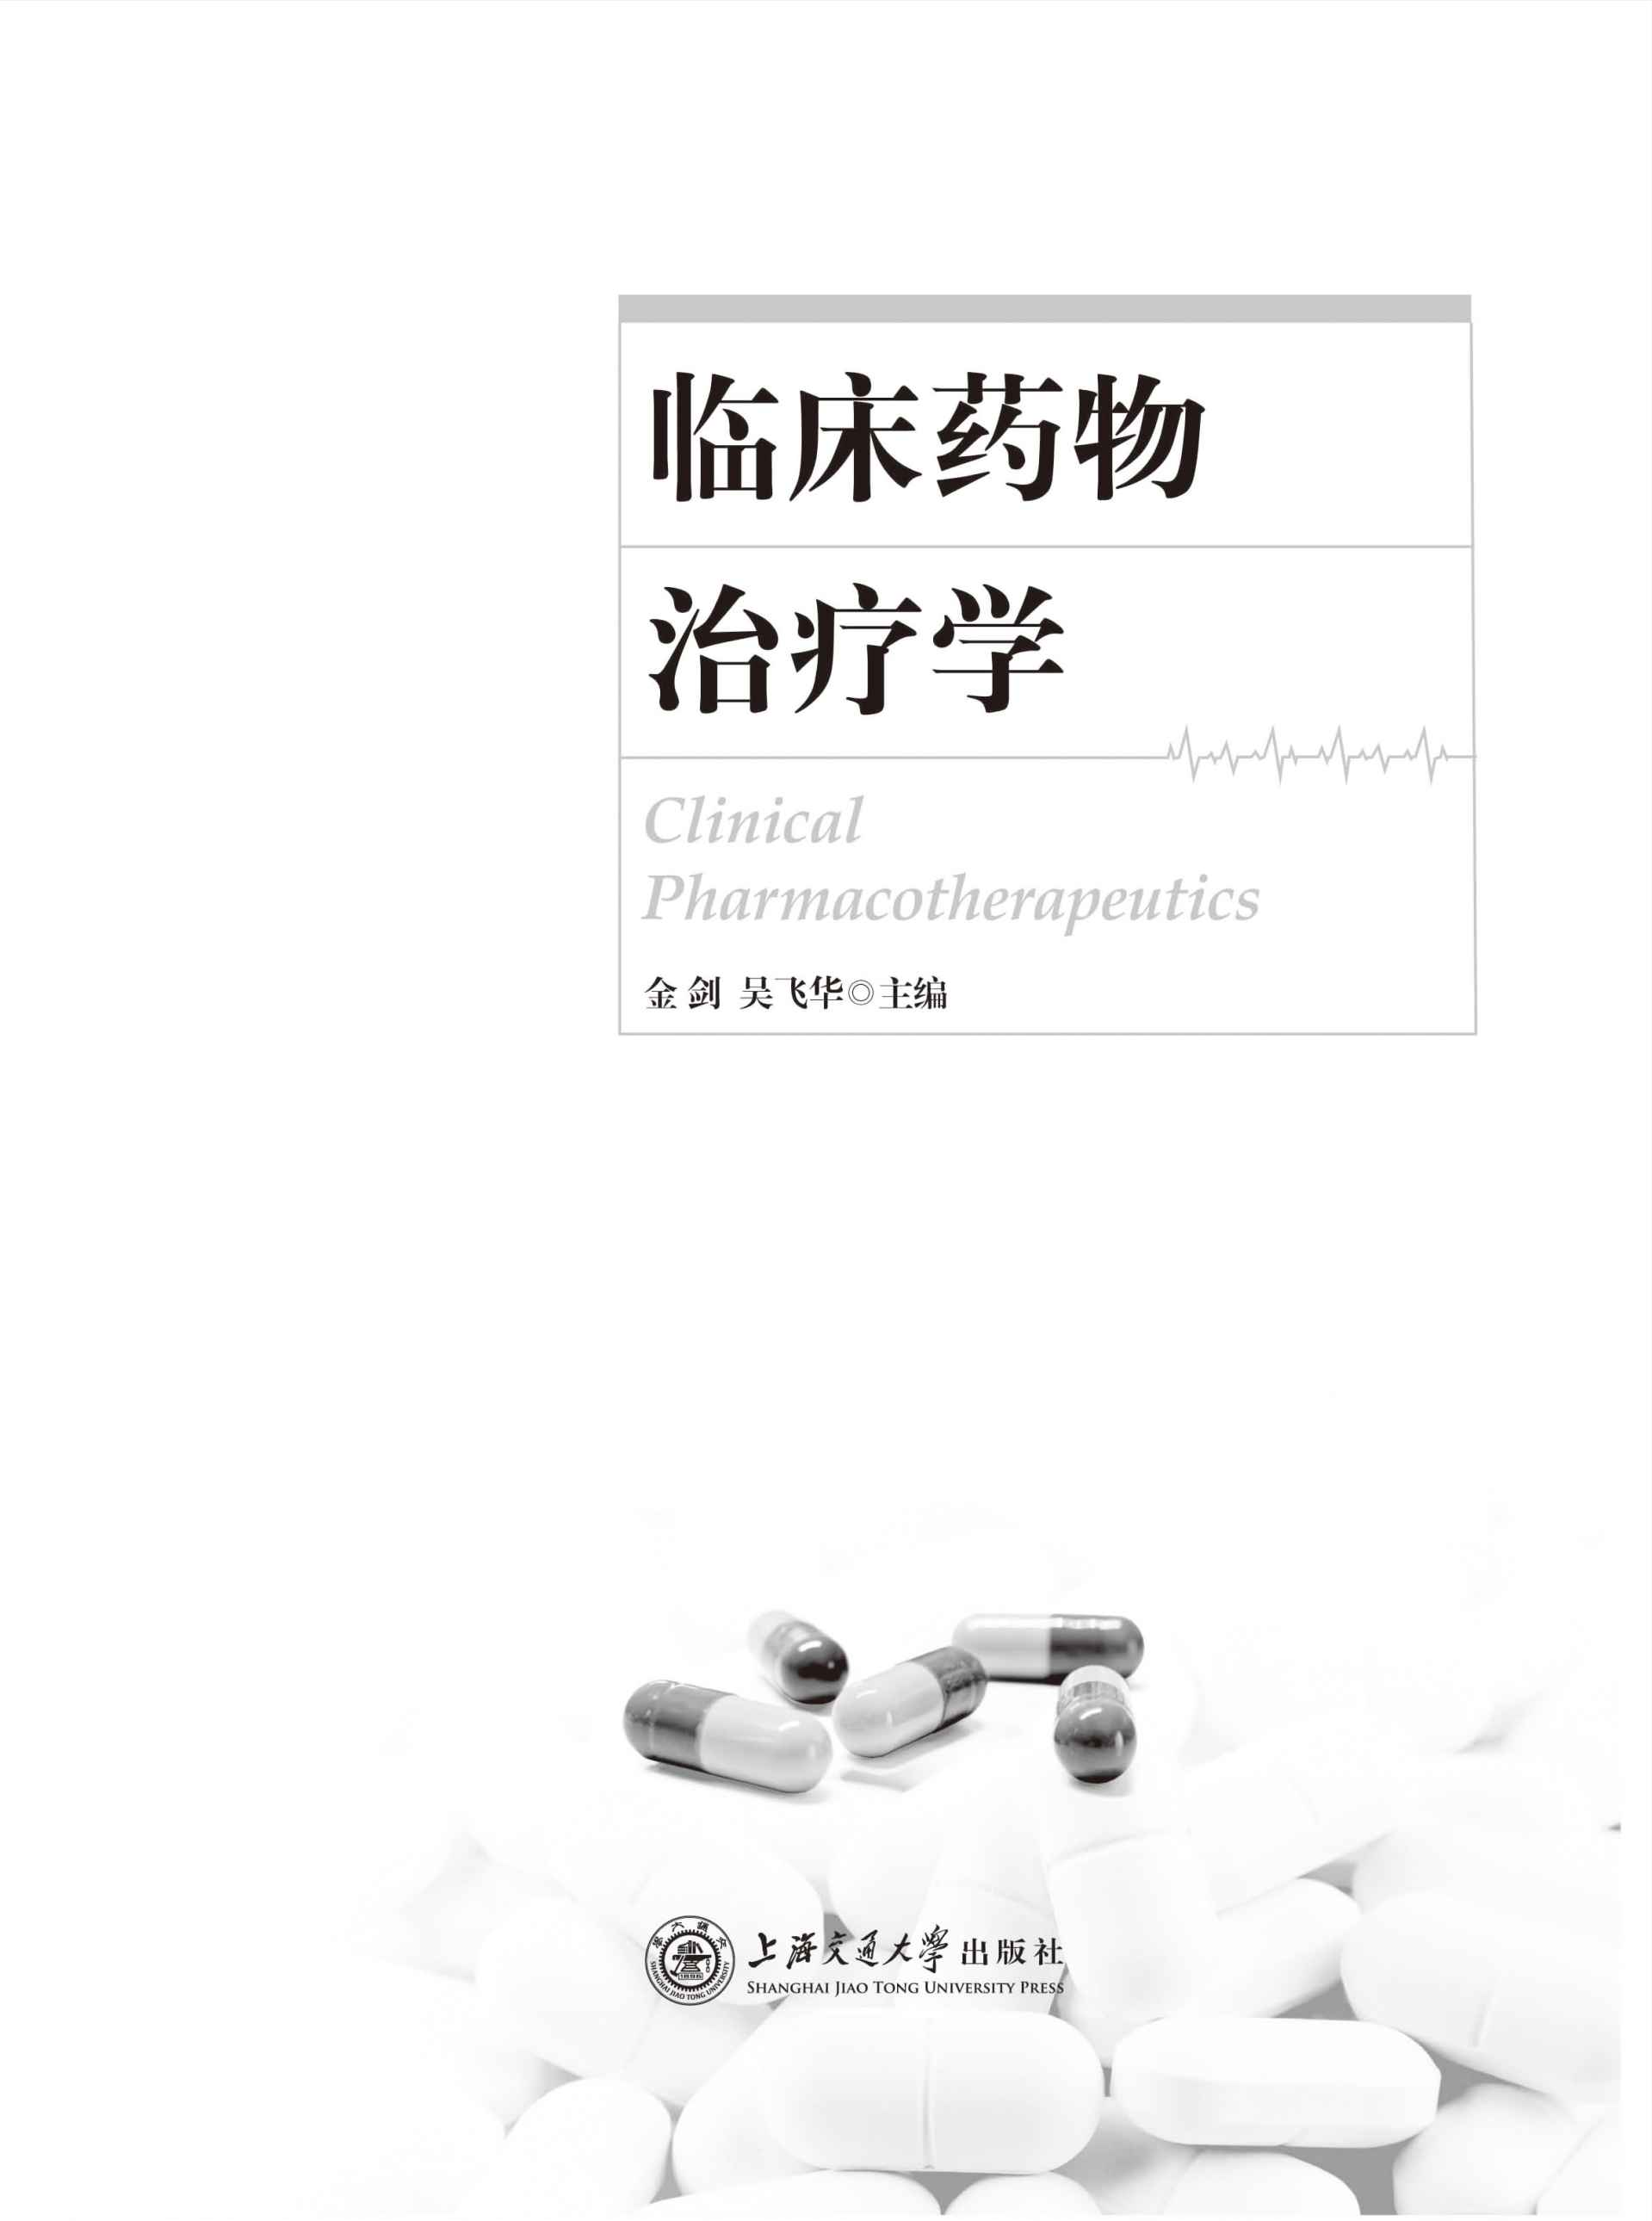
\includegraphics{./images/Image00000.jpg}}

注:以上如有1个问题的回答为“是”,则进行第二步筛查;如每个问题的回答都为“否”,病人在以后每周进行1次初步筛查。
\end{table}



\begin{table}[htbp]
{\centering
\caption{第二步正式筛查}
\label{tab1-2}
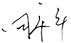
\includegraphics{./images/Image00001.jpg}}

{注:NRS 2002的制定依据现有的随机临床试验}

{*表明确诊的病人可直接归为此类。用黑体字标注的病例按照下面介绍的疾病严重程度标准进行归类:}

{营养不良危险因素是指机体目前的营养状况以及因此可能导致的机体损害,因为在病理状况下机体代谢压力加大,对营养素的需要量也有所增加。}

{营养干预对于下列病人是必需的:}

{1)严重的营养不良(3分);}

{2)严重疾病(3分);}

{3)中度营养不良+轻度疾病(2分+1分);}

{4)轻度营养不良+中度疾病(1分+2分)。}

{1分:病人患有慢性疾病并因并发症而住院,身体虚弱但可以定时下床活动。病人对蛋白质的需要量增加,但对于大多数病例通过正常膳食或口服营养素补充剂就可以满足需要。}

{2分:病人卧床休息,如胃部外科大手术。病人对蛋白质的需要量大大增加,一些病人必须通过人工喂养才能满足需要。}

{3分:重症监护病人,如使用呼吸机的病人。病人对蛋白质的需要量增加,并且通过人工喂养也不能满足需要。蛋白质分解和氮丢失显著减少。}
\end{table}



\hypertarget{text00002.htmlux5cux23mllj4}{%
\section{营养评价内容及方法}\label{text00002.htmlux5cux23mllj4}}

\hypertarget{text00002.htmlux5cux23mllj5}{%
\subsection{疾病及饮食史}\label{text00002.htmlux5cux23mllj5}}

疾病史包括急、慢性疾病回顾以及既往营养丢失情况。饮食史多采用24小时膳食回顾或3天连续食物称重法,应该同时考虑食物的数量和质量,将能量、蛋白质和微量营养素与推荐摄入量(DRIs)进行比较。Beck使用体重和食欲下降对入院病人进行初筛,然后通过主观全面评价法对营养不良疑似病人进一步评价,发现其中营养不良比例高达63%。膳食评价可以在病人入院早期发现营养问题,给予营养支持,改善病人预后。

\hypertarget{text00002.htmlux5cux23mllj6}{%
\subsection{体格测量}\label{text00002.htmlux5cux23mllj6}}

{1.体重}
 体重是临床上最常用的体格检查指标,但目前还没有完全做到记录每个住院病人的体重。短期体重变化是反映体液平衡的最佳指标。较长期的体重改变能够反映总体营养状况改变,根据病前3~6个月的体重变化或实际体重占理想体重的百分比,来判断是否需要进一步检查评估。3个月内非自愿的体重减轻是评价机体营养状况的有用指标,体重减轻<5%为轻度,体重减轻>10%为重度。如果病人体重持续减轻,临床医师应该对此警惕并找出原因。在儿科病人中,联合应用体重和身高,可以转换成多种指标对营养状况进行监测,如身高别体重(W/H)可以判断是否存在急性营养不良及其程度,年龄别身高(H/A)用来判断是否存在慢性营养不良及其程度。身高别体重比年龄别体重更能反映近期或进行性体重丢失,与预后相关,而年龄别体重(W/A)低下并不会导致患儿死亡率的明显升高。

体质指数(BMI)是目前临床上常用的另一项体重/身高关系指数,等于体重与身高平方的比值,多用于成人或肥胖儿童营养评价。亚洲人的BMI
18.5~24为正常,>24为超重,<18.5为营养不良,<14为严重营养不良,这种病人存活的可能性很小。个体BMI不仅要与以上标准进行比较,而且还要与本人近期的数值进行比较,这样意义会更大。Tienboon将BMI应用于身高<145cm的儿童,如BMI在13.0~14.5代表轻度营养不良,11.5~12.9为中度营养不良,<11.5为重度营养不良。

{2.皮褶厚度测量}
 可用来估计体脂含量,因为总体脂肪和某些特定部位的皮褶厚度之间存在一定的比例关系,通常选择测量上臂肱三头肌皮褶厚度(TSF),其次是选择肩胛下角处皮褶厚度。慢性营养不良的病人常见有皮褶厚度的减低。由于重症病人TSF受总体脂肪变化的影响,而且不同人群由于年龄、性别及疾病的不同,皮下脂肪与总体脂肪的比值可以在0.2~0.7之间变动,测量精确性差,往往高估消瘦病人的体脂含量,而低估肥胖者的体脂含量。不同部位皮褶厚度测量值之和可以更为准确反映病人体脂含量。

{3.中臂围(MAC)}
 是用卷尺测量肩峰和尺骨鹰嘴中点的手臂围,这个指标易测量且误差也较小。中臂围与某些疾病的死亡率、发病率等指标有很好的相关性,它主要是测量身体的总成分,包括肌肉、骨骼、体液和脂肪组织等,当蛋白质及脂肪储备下降时MAC迅速减少。根据TSF和MAC可以计算中臂肌围、臂脂肪面积、臂肌面积,用于反映脂肪和瘦体组织含量。

{4.头围(HC)}
 HC是3岁以内儿童生长发育和营养状况评价的常用指标,可以间接反映大脑发育情况,如婴儿期头围增长缓慢,将来出现发育问题的风险明显增高。中臂围与头围比值(MAC/HC)受体液变化的影响较小,是新生儿、婴儿营养评价及监测中筛选营养不良的敏感指标。

\hypertarget{text00002.htmlux5cux23mllj7}{%
\subsection{生化指标}\label{text00002.htmlux5cux23mllj7}}

(一)蛋白质营养状况

{1.白蛋白}
 白蛋白的代谢半衰期是18天,所以其代谢变化对浓度的影响需要一段时间才能显现出来。白蛋白从血液中正常流失的速度是其合成速度的10倍。营养不良的病人,机体内脏蛋白储备丧失,血浆蛋白尤其是快速转化蛋白多有降低。血浆白蛋白是评价营养状况的常用指标,白蛋白浓度明显降低常常导致感染发生率和死亡率增高。

{2.前白蛋白和转铁蛋白}
 前白蛋白和转铁蛋白半衰期短,前者为2天,后者为7天,它们对营养状况变化敏感,是判别蛋白质营养不良的良好指标。实验证明,血清前白蛋白浓度在肠外营养应用1周后明显升高(P<0.001),而应用白蛋白则无改变。Staffan对28位极低体重出生儿进行11种血浆蛋白质测定,发现前白蛋白、转铁蛋白、视黄醇结合蛋白最适合该人群蛋白质营养状况评价。

{3.纤维连接蛋白}
 纤维连接蛋白在饥饿状态下迅速降低,给予营养补充后很快恢复正常,因此也可以作为营养评价的指标。

{4.血红蛋白}
 营养性贫血是最常见的营养问题,美国第三次营养与健康调查发现1~3岁儿童缺铁性贫血发生率为15%。上海新华医院对上海3家儿科医院进行调查,贫血发生率为29.3%。血红蛋白和血细胞比容测定可以诊断营养性缺铁性贫血,转铁蛋白浓度与总体铁储备密切相关,是正常人体铁状况的敏感指标。为病人进行血常规检查,对营养状况评价很有意义。

{5.肌酐}
 肌酐主要由肌氨酸代谢分解产生,因此尿肌酐清除率可作为估计瘦体组织的可靠指标。肌酐身高指数(CHI)常用来估计肌肉蛋白质储备,CHI在60%~80%为中度蛋白质缺乏,<60%为重度蛋白质缺乏。

{6.其他}
 3-甲基组氨酸测定结果也可以反映肌肉蛋白储备和运转情况,但它和肌酐清除率都存在一定问题,如难以准确收集24小时尿量,受饮食和肾功能影响很大,尚不推荐常规应用。肝脏中酶的活性以及电解质水平(钙、磷、镁等)都应常规检测。锌、硒和铁的检测对于胃肠道病人尤其重要。

(二)免疫功能测定

慢性阻塞性肺病(COPD)病人的营养状况与其细胞免疫功能密切相关,一般把免疫功能的评价作为营养状况评价的重要组成部分。

{1.外周血总淋巴细胞计数}
 外周血总淋巴细胞计数(TLC)指外周血中总淋巴细胞的数量,可反映细胞免疫功能。TLC=白细胞×淋巴细胞百分比,正常值≥1.5×10\textsuperscript{9}
/L,营养不良时TLC下降。

{2.迟发型超敏皮肤试验}
 于前臂屈侧皮内注射不同的抗原制剂0.1ml,待48小时测量接种处硬结直径。常用的抗原包括链激酶、腮腺炎病毒、白色念珠菌提取液、植物血凝素、结核菌素纯蛋白衍生物等。营养不良时细胞免疫功能受损,迟发型超敏皮肤试验为无反应或反应减弱,即接种处不出现硬结或硬结直径很小。

{3.外周血T细胞亚群}
 机体T细胞的免疫应答反应对抵抗力或免疫功能非常重要,其中目前临床上常用的指标主要是$\text{CD}^+_3$
、$\text{CD}^+_4$
、$\text{CD}^+_8$
、$\text{CD}^+_4$
/$\text{CD}^+_8$ 等,营养不良时下降。

\hypertarget{text00002.htmlux5cux23mllj8}{%
\subsection{机体组成测定}\label{text00002.htmlux5cux23mllj8}}

构成机体的基本化学成分是蛋白质、脂质、碳水化合物、无机盐和水等。由于中性脂肪并不结合水和电解质,假设人体去脂体质(fat-free
mass, FFM)或瘦体群(lean body mass,
LBM)的组成是恒定的,那么通过分析其中一种组成(如水、钾或钠)的量可估计FFM的多少,然后用体重减去FFM的重量即为体脂(body
fat,
BF)。因此,机体的组成按照二元件模型可分为BF和FFM两部分。FFM可再分为体细胞群(body
cell mass, BCM)和细胞外群(extracellular mass,
ECM)。BF是机体储备能量的主要组织,约占体重的25%,其主要成分是脂肪。脂肪中仅有1.0kg脂肪为生命活动所必需,其余可在需要时被动员用于能量消耗。BCM是能够利用氧进行代谢活动的组织,约占人体总重量的40%。ECM主要是细胞外支持组织,用于支持细胞的功能和活动,约占人体重量的35%。在人体组成分析中,显然FFM较BF在生命活动和机体代谢方面更具有重要作用。测定人体组成及其变化比单纯体重指数更能客观反映病人实际的营养状况。

早在1940年,水中称重法应用于人体机体组成测定,来推算体脂和去脂体质的重量。空气置换体积描记术是一项新的密度测定方法,尤其适合那些无法耐受水中密度测定的儿童等特殊病人,David等在9~14岁儿童中应用发现该法比水中称重等方法能更精确测定体脂含量。因为水与钾仅存在于瘦体组织,且含量相对恒定,脂肪不含水和钾。因此通过放射性核素稀释法总体水测定和总体钾测定都可以计算总体脂肪和廋体组织含量。双能X线吸收法是测定人体骨骼无机盐、体脂、去脂组织等机体组成的常用方法,与总体钾测定相关性较好。但多用于研究机构,较少应用于临床评价。迟发性中子激活分析法能够测定氮、钠、氯、钾、钙、磷等多种原子的绝对水平,如测定总体氮可用于机体蛋白质组成分析。CT及磁共振能获得体脂分布的精确图像。

许多机体组成测定方法由于存在一些缺点,如费用昂贵、放射暴露、需要专门的测量仪器和场所,或是需要检查对象合作,而难以在临床上推广引用。生物电阻抗法(BIA)是近年来广泛用于机体组成测定的新方法,具有可床边进行,操作简便、快捷、安全、无创等优点。它的原理是利用不同生物组织对电流导电的差异性,低频电流主要通过细胞外液传导,高频电流可以穿透细胞膜,同时通过细胞内液和细胞外液,推测组织各部分的含量。基于此特性可推测总体水、瘦体组织、细胞外液和细胞团块等多种机体组成成分。Phillips使用BIA和放射性核素稀释法两种方法对青春期女性进行测定,认为BIA法能精确反映她们月经前和月经后去脂组织和体脂含量变化。

\hypertarget{text00002.htmlux5cux23mllj9}{%
\subsection{营养平衡研究}\label{text00002.htmlux5cux23mllj9}}

营养平衡研究一直用于营养评估,通过计算出入量,可进行氮、无机盐、维生素、微量元素等多种物质的平衡研究。氮平衡测定是一项重要的营养平衡研究方法,可直接判断蛋白质摄入情况,常用于营养治疗过程中观察病人的营养摄入是否足够以及了解分解代谢的演变。氮平衡首先测量人体通过尿液、粪便、皮肤以及其他途径(汗液、分泌液等)流失的氮,将摄入氮减去以上各种途径排出的氮就可以计算出氮平衡。为了确定蛋白质的需要量,氮平衡测定需在蛋白质从缺乏到过剩几种不同的摄入水平下进行。每个摄入水平的测定都需要持续几天,使机体保持代谢稳定。由于技术上的原因,目前按照以上要求进行的代谢试验较少,仍缺乏可用于临床病人的标准化方法。正氮平衡常常意味着预后改善,病人营养支持的目的是达到正氮平衡。但氮平衡不能反映机体的蛋白质储备或营养状态,需结合机体组成等测定综合评价。

\hypertarget{text00002.htmlux5cux23mllj10}{%
\subsection{复合型营养评定方法}\label{text00002.htmlux5cux23mllj10}}

{1.主观全面营养评估法(SGA)}
 SGA是Detsky在1987年首先提出,是根据病史和体格检查的一种主观评估方法,特点是以详细的病史与临床检查为基础,省略人体测量和生化检查。其理论基础是:身体组成改变与进食改变、消化吸收功能的改变、肌肉的消耗、身体功能及活动能力的改变等相关联。在重度营养不良时,SGA与身体组成评定方法有较好的相关性。此方法简便易行,适于在基层医院推广(表1-3)。

\begin{table}[htbp]
\centering
\caption{营养状态的SGA(subjective global assessment)评估内容和指标}
\label{tab1-3}
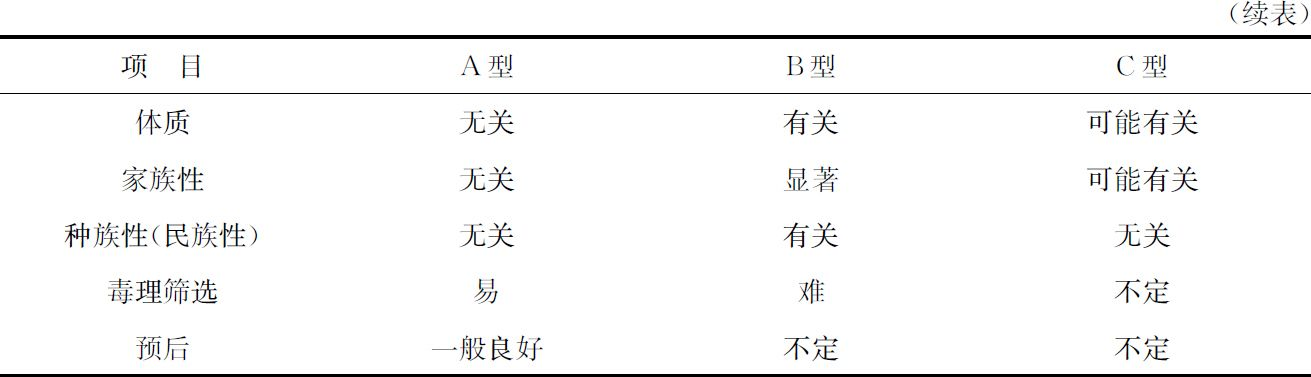
\includegraphics{./images/Image00005.jpg}
\end{table}

{2.预后营养指数(PNI)}
 PNI是由Mullen等对4种营养状态评价参数与外科手术病人预后的相关性进行了分析统计之后提出来的一种综合性营养评价方法。

PNI(%)=158-16.6(ALB)-0.78(TSF)-0.20(TFN)-5.80(DHST)

式中ALB为血清白蛋白(单位:g%);TSF为三头肌皮褶厚度(单位:mm);TFN为血清转铁蛋白(单位:mg%);DHST为迟发性超敏皮肤反应试验(硬结直径>5mm者,DHST=2;硬结直径<5mm者,DHST=1;无硬结反应者,DHST=0)。

评定标准:若PNI<30%,表示发生术后并发症及死亡的可能性均很小;若30%≤PNI<40%,表示存在轻度手术危险性;若40%≤PNI<50%,表示存在中度手术危险性;若PNI≥50%,表示发生术后并发症及死亡的可能性均较大。

Mullen等对161例非急诊手术病人的PNI测定调查显示,手术危险增加与术后并发症发生率及死亡率升高相关,其灵敏度为86%,特异性为69%。

{3.微型营养评定(MNA)}
 是一种简单、快速,适用于评价病人(特别是老年人)营养状况的方法,由Guigoz、Vallas和Garry于1994年提出。MNA评价内容包括: ①人体测量;②整体评定;③膳食问卷;④主观评定等。各项评分相加即得MNA总分。具体评价问卷内容如下所列(见[附])。

\begin{center}\rule{0.5\linewidth}{\linethickness}\end{center}

[附]

营养评价问卷

(一)姓名 性别 出生 年 月 日

(二)家庭住址

(三)原有疾病

(四)体重(kg) 身高(m) 血压(mm Hg)

1.筛选(按不同程度给予量化评分)

(1)既往3个月内是否有食欲下降、消化问题、咀嚼或吞咽困难而摄食减少?

0=食欲完全丧失□ 1=食欲中等度下降□ 2=食欲正常□

(2)既往3个月内体重下降

0=>3kg□ 1=不知道□ 2=1~3kg□ 3=无体重下降□

(3)活动能力

0=需卧床或长期坐着□ 1=能不依赖床或椅子,但不能外出□ 2=能独立外出□

(4)既往3个月内有无重大心理变化或急性疾病?

0=有□ 1=无□

(5)神经心理问题

0=严重智力减退或抑郁□ 1=轻度智力减退□ 2=无问题□

(6)BMI(kg/m\textsubscript{2} )

0=<19□ 1=19~<21□ 2=21~<23□ 3=≥23□

筛选总分(14):≥12正常,无需以下评价;≤11可能营养不良,继续以下评价

2.评价

(1)独立生活(无护理或不住院)?

0=否□ 1=是□

(2)每天应用处方药3种?

0=是□ 1=否□

(3)压疮(褥疮)或皮肤溃疡?

0=是□ 1=否□

(4)每天几次吃完全部饭菜?

0=1餐□ 1=2餐□ 2=3餐□

(5)蛋白质摄入情况:

*每天至少一份奶制品? A是□ B否□

*每周2份以上菜果或蛋? A是□ B否□

*每天肉、鱼或家禽? A是□ B否□

0.0=0或1个“是”□

0.5=2个“是”□

1.0=3个“是”□

(6)每天2份以上水果或蔬菜?

0=否□ 1=是□

(7)每天饮水量(水、果汁、咖啡、茶、奶等):

0.0=<3杯□ 0.5=3~5杯□ 1.0=>5杯□

(8)喂养方式:

0=无法独立进食□ 1=独立进食稍有困难□ 2=完全独立进食□

(9)自我评定营养状况:

0=营养不良□ 1=不能确定□ 2=营养良好□

(10)与同龄人相比,你如何评价自己的健康状况?

0.0=不太好□ 0.5=不知道□ 1.0=好□ 2.0=很好□

(11)中臂肌围(cm):

0.0=<21□ 0.5=21~22□ 1.0=≥22□

(12)腓肠肌围(cm):

0=<31□ 1=≥31□

评价总分(16):

筛选总分:

总分(30):

MNA分级标准:上述各项评分相加,若MNA≥24,表示营养状况良好;若17≤MNA≤23.5,表示存在发生营养不良的危险;若MNA<17,表示有确定的营养不良。

\begin{center}\rule{0.5\linewidth}{\linethickness}\end{center}

{4.住院病人预后指数(HPI)}

HPI=0.92(ALB)-1.00(DH)-1.44(SEP)+0.98(DX)-1.09

式中:ALB为血清白蛋白(单位:g/L);DH为延迟超敏皮肤试验(有1种或多种阳性反应,DH=1;所有均呈阳性,DH=2);SEP:败血症(有败血症,SEP=1;无败血症,SEP=2);DX表示诊断患有癌症(有癌,DX=1;无癌,DX=2)。

评价标准:若HPI为+1,表示有75%的生存概率;若HPI为0,表示有50%的生存概率;若HPI为-2,表示仅有10%的生存概率。

{5.营养风险指数(NRI)}
 美国退伍军人协会肠外营养协作研究组(VATPNCSG)于1991年在《新英格兰医学杂志》上首先提出NRI评价方法。NRI=10.7(ALB)+0.0039(TLC)+0.11(Zn)-0.044(Age)。

式中:ALB为血清白蛋白;TLC为淋巴细胞计数;Zn为血清锌水平;Age为年龄。

评定标准:若NRI>60,表示危险性低;若NRI≤55,表示存在高危险性。

Clugston等于2006年对梗阻性黄疸病人的研究表明,NRI风险升高与住院时间延长和死亡率增加相关。

完整的营养评价包括:疾病及饮食史、体格测量、生化指标、机体组成、营养平衡研究等。在营养评价过程中,体格测量与生化指标是营养评价的最常用方法,具有简单、方便、重复性好、能提供定量资料、不需要特殊仪器等特点。很多测量值与机体组成营养状况分析在统计学上具有显著相关性。然而,简单的体格测量和实验室检查常不能体现营养状况的急性改变,不能反映轻度和中度营养不良,也就不足以作为营养评价的唯一方法。同时,由于置信限较宽,敏感性和特异性差,更适用于流行病学人群调查,评价特定人群的营养状态。近年来,为了提高营养评价方法的敏感性和特异性,人们结合预后和大量的营养学指标,通过多因素回归分析,选择其中有意义的参数,组成最佳的预测模式,建立了多种营养评价方法,为营养状况评价提供了定性、定量的可信指标。

{参考文献}

[1]陶晔璇,徐远飞,汤庆娅,等.儿科病人入院时营养状况评价.中国临床营养杂志,2007,15(4):214~217

[2]蔡威.临床营养基础.第3版.上海:复旦大学出版社,2004,61~18

[3]Tienboon P. Nutrition problems of hospitalised children in a
developing country: Thailand. Asia Pacific J Clin Nutr, 2002, 11 (4):
258~262

[4]Renaudin P. Evaluation of the nutritional status of children less
than 5 years of age in Moundou, Chad: correlations with morbidity and
hospital mortality. Article in French. Med Trop(Mars), 1997, 57 (1):
49~54

[5]Hendricks KM, Duggan C, Gallagher L, et al. Malnutrition in
hospitalized pediatric patients. current prevalence. Arch Pediatr
Adolesc Med, 1995, 149: 1118~1122

[6]Ogden CL, Flegal KM, Carroll MD, et al. Prevalence and trends in
overweight among US children and adolescents, 1999~2000. JAMA, 2002,
288 (14): 1728~1732

[7]Ah SM, Selwyn BJ, Luby S, et al. Prevalence and correlates of
stunting among children in rural Pakistan. Pediatr Int, 2003, 45 (1):
49~53

[8]Jacobs DO, Wong M. Metabolic assessment. World J Surg, 2000, 24
(12): 1460~1467

[9]Phillips SM, Bandini LG, Compton DV, et al. A longitudinal
comparison of body composition by total body water and bioelectrical
impedance in adolescent girls. J Nutr, 2003, 133 (5): 1419~1425

[10]Kuczmarski RJ, Ogden CL, Guo SS, et al. 2000 CDC growth charts for
the United States: methods and development. Vital Health Stat 11, 2002,
(246): 1~190

[11]Ronald E. Pediatric nutrition handbook. 6th ed. American: American
Academy of Pediatrics, 2009, 559~576

\protect\hypertarget{text00003.html}{}{}


\chapter{颅脑}

\section{检查方法}

\subsection{常规检查}

横断面(或轴位)扫描:病人仰卧,有3个主要扫描平面。其扫描基线为:①听眦线(orbitomeatal
line,OML):亦称为眶耳线,简称OM线,即外眦至外耳孔中点的连线。②听眉线(superior
orbitomeatal
line,SML):亦称为上眶耳线,简称SM线,即眉毛上缘中点与外耳孔中点的连线。③瑞氏基底线(reid's
base
line,RBL):亦称人类学基线,简称RB线,即眶下缘与外耳孔中点的连线。检查幕上病变常用OM线;幕下病变常用SM线;眶内病变常用RB线。

冠状面扫描:病人仰卧或俯卧位,头部过伸,使冠状面与OM线垂直扫描。

\subsection{增强扫描}

一般认为,对急性颅脑外伤、急性卒中可只做平扫;对于脑瘤术后复查或只有增强检查才能显示病变的复查病例可只行造影增强;对于脑肿瘤、脑血管疾病、感染性疾病均需做增强扫描,外伤患者平扫正常时亦可行增强扫描。一般造影剂用量为60~100ml或儿童以2ml/kg用量,团注或快速滴注。

其显影机制分为两类:①血管内显影:如动脉瘤、动静脉畸形,其显影时间短,应注药后扫描或边注边扫。②血管外显影:强化机制在于血脑屏障的破坏(如胶质瘤)或血供丰富(如脑膜瘤、听神经瘤、脓肿壁)。由于垂体血供丰富,垂体增强扫描有利于缺乏血供的垂体瘤尤其微腺瘤的检出。

\subsection{脑池造影CT扫描}

造影剂可应用阳性非离子型水溶性碘造影剂(伊索显和欧乃派克等)和阴性造影剂(空气),后者主要用于小听神经瘤的诊断。一般阳性造影剂的用量为8~10ml,空气3~5ml,经腰穿注入。水溶性造影剂取头低脚高位或病变侧在低下部位,气体反之。一般注入造影剂15分钟后扫描,观察脑室多于6小时后扫描,延时的目的在于降低碘液浓度。如欲观察脑脊液的动力变化,则于注入造影剂2小时、6小时、12小时和24小时后进行扫描,必要时可于48小时或72小时后扫描。

\subsection{脑CT血管成像}

脑部CT血管成像或称为脑部CT血管造影(CT
angiography,CTA),是指经静脉注入造影剂后利用CT对包括靶血管在内的受检层面进行连续的薄层立体容积扫描,然后进行图像后处理,最终使靶血管立体显示的血管成像技术。

扫描从后床突下30mm开始,向上达后床突上50~60mm。其常用扫描参数如下:螺距1~2,层厚1~2mm,重建间隔1mm,造影剂用量(300mg/ml)80~120ml,注射流率2.5~3.5ml/s,延迟时间15~25秒。双层或多层螺旋CT可增加螺距、减小层厚,以取得更优质的图像。图像后处理可采用MIP、SSD和VR,以MIP最常用。

脑CT静脉成像(CT venography,CTV)扫描方法同上,只是扫描延迟时间为40秒。

CTA(包括CTV)可用于显示脑底动脉环(willis环)和大脑前、中、后动脉主干及其2~3
级分支血管;CTV
可显示大脑内静脉、大脑大静脉、皮质静脉、上矢状窦、直窦、横窦和乙状窦等。CTA(包括CTV)可用于动脉瘤、血管畸形(主要是AVM)、肿瘤血管、静脉病变及头皮血管瘤等的诊断。

\subsection{脑CT灌注成像}

CT灌注成像在中枢神经系统的应用包括:①作为颅外颈动脉或椎动脉闭塞性疾病的功能性检查方法,研究颅内血流量和侧支循环情况。②早期发现梗死或缺血,并显示其范围。③血管炎或继发性蛛网膜下腔出血时估计血管痉挛情况。④AVM估计分流情况。⑤研究肿瘤的血液灌注情况。

\subsubsection{检查技术}

CT灌注成像的质量受造影剂注射的总量、速度、患者的心功能状态以及CT扫描伪迹、部分容积效应等多种因素的影响。扫描时经肘静脉注射加热至37℃的造影剂40~50ml(儿童约为1ml/kg体重)。开始注射造影剂的同时启动快速动态扫描程序,以1层/秒的速度连续扫30~40秒以上,重建30~40幅灌注图像。注射流率多为8~9ml/s,最快达20ml/s,国内有学者采用2.5ml/s也获得较满意的CT灌注图像。通常包括最大强度投影(MIP)图、脑血流量(CBF)图、脑血容量(CBV)图、局部灌注达到峰值的时间(TTP)等图像。这些图像可通过数字化形式存储,均可彩色显示,以突出病变区域的对比度。

\subsubsection{灌注参数}

1.脑血容量(cerebral blood
volume,CBV):是指存在于一定量脑组织血管结构内的血容量,单位为ml/100g。根据时间-密度曲线下方封闭的面积计算得出。

2.脑血流量(cerebral blood
flow,CBF):CBF=CBV/MTT,指在单位时间内流经一定量脑组织血管结构的血流量,单位为ml/(100g·min)。它反映脑组织的血流量,CBF值越小意味着脑组织的血流量越低。正常值一般>50~60ml/(100g·min),<10~20ml/(100g·min)将导致膜泵衰竭和细胞死亡。

3.平均通过时间(mean transit
time,MTT):开始注射造影剂到时间-密度曲线下降至最高强化值一半的时间,主要反映的是造影剂通过毛细血管的时间,单位为秒(s)。

4.峰值时间(time to
peak,TTP):为开始注射造影剂至强化达到峰值的时间,由时间-密度曲线测得,单位为秒(s)。

此外,还有表面通透性(permeability of surface,PS)等参数。

\section{正常解剖和CT表现}

\subsection{颅盖软组织(头皮)}

颅盖软组织在额、顶、枕部分为皮肤、皮下组织、帽状腱膜、帽状腱膜下层和颅骨骨膜5层。前3层紧密连接,CT不能识别。帽状腱膜下层由疏松结缔组织构成,内含少量血管,CT呈低密度带,头皮裂伤出血亦在此层,如有化脓感染可蔓延到整个颅顶,并可经导静脉扩散到颅内。颅盖软组织在颞部则由皮肤、皮下组织、颞浅筋膜、颞深筋膜、颞肌和颅骨骨膜6层构成。

颅骨外膜CT不能识别,在颅缝处连接紧密并深入缝间成为缝间膜,故骨膜下血肿不超过此缝,并可据此与帽状腱膜下血肿相鉴别。

\subsection{脑颅骨和颅缝闭合的时间及顺序}

脑颅骨由枕骨、额骨、蝶骨、筛骨各一块及颞骨、顶骨各两块组成。颅骨分为3层,即外板、板障和内板。成人内外板CT表现为高密度,CT值>250Hu。新生儿板障为低密度,随年龄增长密度增加,50岁后板障层钙化与内外板融合为一层致密层。成人颅缝宽约0.5
mm。新生儿各骨之间为一片等密度的结缔组织膜相连,称为囟。

颅缝闭合约在30岁以后开始。一般矢状缝先闭合,继为冠状缝。而人字缝和枕骨乳突缝闭合最晚,且可终生不闭合。额缝在出生6个月后开始闭合,而在5~6岁时应完全闭合,此缝亦可终生存在。颅底缝多在出生时闭合,只有蝶枕缝到青春期闭合。

此外,应注意识别脑膜中动脉、板障静脉沟、静脉窦、导静脉、蛛网膜颗粒等常见的脉管压迹,以免误诊为骨折。

\subsection{颅底各颅窝的特点和孔道}

颅底骨内面由蝶骨嵴和颞骨岩部嵴分为前、中、后颅窝。

\subsubsection{各颅窝的结构特点}

1.前颅窝:筛骨板菲薄,外伤易造成骨折、损伤嗅神经及形成脑脊液漏。额骨眶板上面凹凸不平,脑外伤时底部的滑动易引起脑挫伤。

2.中颅窝:孔、洞较多,外伤骨折或肿瘤破坏通过这些结构引起相应的症状。如骨折累及蝶窦出现鼻出血、脑脊液鼻漏;岩锥骨折可损伤面神经和听神经;鼓室盖骨折引起脑脊液耳漏;脑膜中动脉损伤引起硬膜外血肿。

3.后颅窝:有大量肌肉覆盖,骨折较少见。但与颈段相连,可有畸形发生。

\subsubsection{。}

\begin{table}[htbp]
\centering
\caption{颅底主要孔道及内容物}
\label{tab2-1}
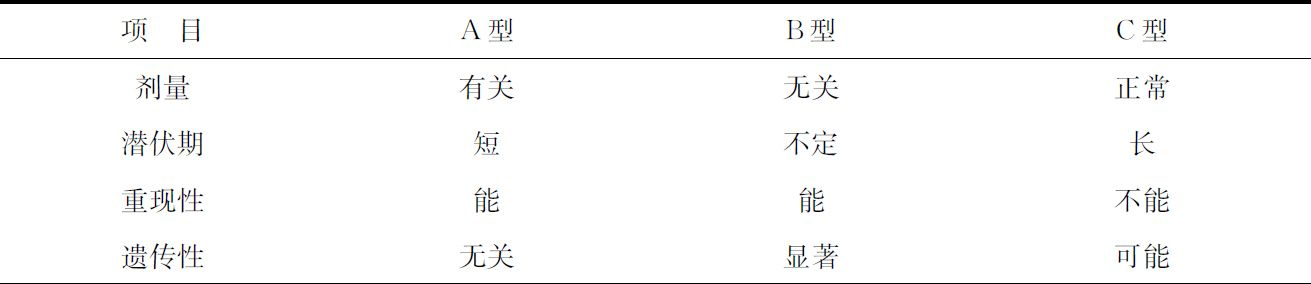
\includegraphics[width=\textwidth,height=\textheight,keepaspectratio]{./images/Image00004.jpg}
\end{table}

\subsection{脑膜}

脑的表面有3层被膜:①软脑膜:紧贴脑的表面,富血管、随脑回起伏。②蛛网膜:位于中层,由薄而透明、疏松成网的纤维构成,无血管结构(故增强扫描无强化),与硬脑膜走行一致。③硬脑膜:位于外层,由致密结缔组织构成,厚而坚韧,与颅骨内面的骨膜完全融合,故通常说硬脑膜为两层结构组成。正常CT不能直接显示3层结构。由于硬脑膜有丰富的血供且无血脑屏障,可以发生明显强化。

硬脑膜内层向颅腔内反折形成双层皱襞有支持、保护作用。主要形成物为:①大脑镰:前端附着于鸡冠,后缘呈水平形与小脑幕相续。大脑镰上、下缘两层分开分别形成上、下矢状窦。轴位像CT呈略高密度线状影,40岁后可钙化。②小脑幕:呈帐篷状分隔大脑枕叶和小脑。后方附着于枕骨横沟,两侧附着于岩椎,上缘正中与大脑镰相续,两侧前内缘形成小脑幕切迹,围绕中脑。轴位呈两侧对称的略高密度影,冠状位呈人字形线状略高密度影。③小脑镰:附着于枕内嵴上的一窄条状突起,分隔小脑半球。④其他:三叉神经半月节(Meckel腔)、海绵窦、直窦、横窦、乙状窦等。

\subsection{蛛网膜下腔和脑池}

脑蛛网膜在脑沟裂处不随之凹入,与软脑膜之间形成宽窄不一的蛛网膜下腔(或称蛛网膜下隙),内含脑脊液。某些局部宽大处称为脑池。主要的有:①大脑纵裂池;②胼胝体池;③小脑延髓池(又称枕大池
);④小脑溪(又称小脑谷);⑤延池;⑥桥池;⑦桥脑小脑角池;⑧脚间池;⑨视交叉池;⑩终板池;⑪外侧裂池;⑫环池;⑬四叠体池;⑭大脑大静脉池;⑮小脑上池(是四叠体池向后的延续);⑯帆间池(又称中间帆腔或第三脑室上池)。

鞍上池为CT和MR等轴位图像所特有。由于扫描体位的影响可呈:①六角星:前角为纵裂前部的后端(紧贴前角后端的横行部分主要是交叉池);两前外侧角为两外侧裂池;两后外侧角为围绕中脑的环池;后角为大脑脚间的脚间池(图\ref{fig2-1})。②五角星:与六角星不同的是,两后外侧角为围绕桥脑上部的桥小脑角池,后角不显示。鞍上池前方是额叶底部直回,两侧壁是颞叶海马钩回,后方为大脑脚或桥脑上部。

\begin{figure}[!htbp]
 \centering
 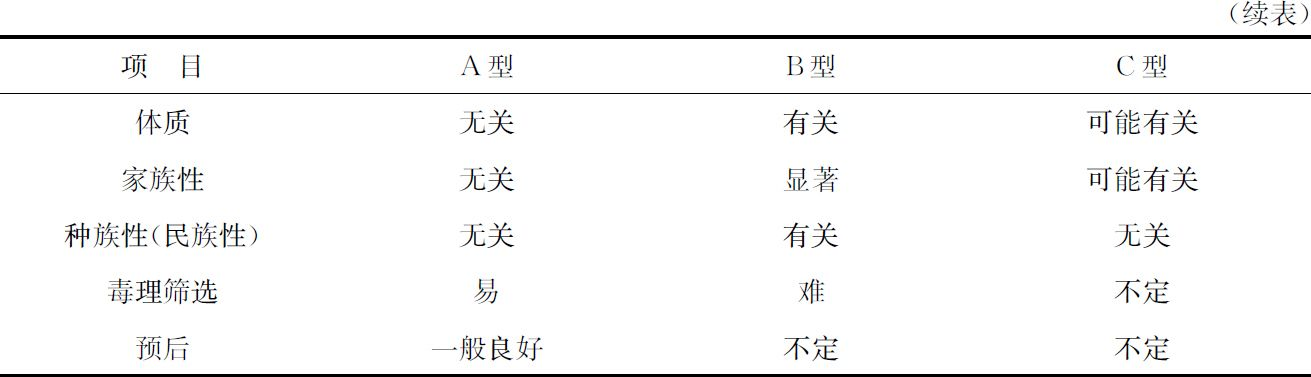
\includegraphics[width=.7\textwidth,height=\textheight,keepaspectratio]{./images/Image00005.jpg}
 \captionsetup{justification=centering}
 \caption{鞍上池 \\{\small 呈六角形水样密度区}}
 \label{fig2-1}
  \end{figure} 



鞍上池内前部可见两条视束,横径约12mm,前后径约8mm,外侧可见两条颈内动脉,中央可见垂体柄,正常垂体柄粗<4mm。

帆间池与第三脑室顶部的区别:帆间池位于第三脑室顶的上方、穹隆体和穹隆连合的下方,呈尖向前的三角区,两前外侧界为穹隆的内侧缘,后界为胼胝体压部。与第三脑室的区别为:①帆间池的层面较第三脑室顶高;②帆间池后界为胼胝体压部,而第三脑室顶部的后界为松果体;③帆间池前部的尖不与侧脑室相连,而第三脑室前端可达侧脑室前角。

此外,枕大池可发育巨大(但一般不产生临床症状)呈对称性和非对称性。结合其有无张力、颅骨有无压迹等可与蛛网膜囊肿相鉴别(图\ref{fig2-2}),有文献将其列入发育异常。因终板较薄不显影,常看到终板池与第三脑室下部相通的假象。小脑溪位于两侧小脑扁桃体之间,呈一细长的间隙,后通小脑延髓池,前通第四脑室。

\begin{figure}[!htbp]
 \centering
 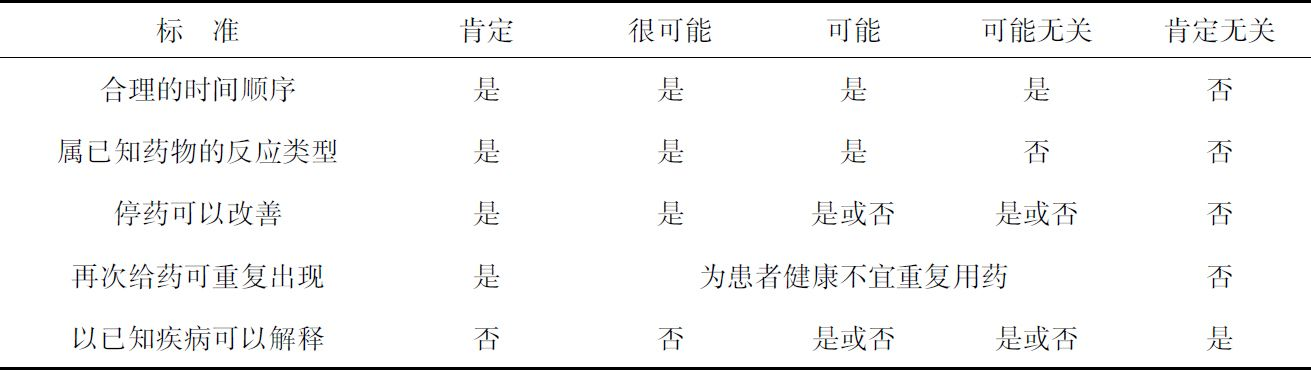
\includegraphics[width=.7\textwidth,height=\textheight,keepaspectratio]{./images/Image00006.jpg}
 \captionsetup{justification=centering}
 \caption{巨大枕大池 \\{\small 显示枕骨内板下至岩锥后缘有新月形水样密度区}}
 \label{fig2-2}
  \end{figure} 


\subsection{大脑半球的分叶及边缘系统}

分叶:大脑由中线的半球间裂分为左右两半,中间由胼胝体相连。大脑半球由脑沟裂分为下列5叶。①额叶:位于前上部。内侧以纵裂和大脑镰与对侧分开,后方由中央沟与顶叶分开,外下方经外侧裂与颞叶分开,前下方为额骨和眶顶。②颞叶:经外侧裂垂直部和水平部与额叶分开。顶枕裂(沟)与枕前切迹(枕极前4~5mm)的连线为颞、枕叶的分界。③顶叶:经中央沟与前方的额叶分开,下方以外侧裂与颞叶分开,后方以顶枕沟与枕叶分开。④枕叶:经顶枕沟与顶叶分开,与颞叶的分界线为顶枕沟与枕前切迹的连线。⑤岛叶:隐藏于外侧裂深部的近三角形的独立区域,四周有环形沟,由额、顶、颞叶皮质沿外侧裂深部凹入形成岛盖。

边缘系统:大脑半球内侧面的扣带回、海马回、钩回、海马、杏仁核等相连构成一个弯弓形脑回,因位置在大脑和间脑交界处的边缘,所以称为边缘系统或边缘叶。通过控制下丘脑来调节内脏及情绪活动。

此外,颞、顶、枕叶的分界线是假设的,因此很不清楚,这一区域也称为颞顶枕交界区。

\subsection{大脑半球的白质}

\subsubsection{半卵圆中心}

髓质占大脑半球的大部分,较厚的皮质下纤维在横断面图像、侧脑室上层面呈半卵圆形,故称为半卵圆中心,是影像学的一个概念。

\subsubsection{大脑白质纤维分类}

大脑白质的纤维结构复杂,大体分为以下3种:

1.联络纤维:在一侧半球内部各回、各叶间的往返纤维称为联络纤维。短的是联系在相邻脑回之间的弓状纤维;长的是联系在各叶皮质间的纤维,如钩束、扣带束、上纵束、下纵束及枕额上、下束等。

2.连合纤维:指联系左右半球的纤维,主要有胼胝体、前联合和海马联合等。①胼胝体:位于大脑纵裂底部,呈拱桥状。前端弯向腹后方称嘴,由嘴向前上方弯曲部称为膝,由膝向后延伸为体部(构成侧脑室壁的大部分),后端较厚称为压部。②前联合:位于胼胝体嘴的后下方,呈卵圆形,是两半球的嗅球和海马旁回的联合。

3.投射纤维:大脑皮层与其下部的间脑、基底节、脑干和脊髓的连接纤维称为投射纤维。包括内囊、穹隆、外囊和最外囊。①内囊:两侧内囊横断面呈“><”型,中央顶点为膝,前后分别为前肢和后肢。内囊位于丘脑、尾状核和豆状核之间。内囊后肢边缘模糊的低密度区(约位于膝部到豆状核后缘距离的2/3~3/4处)为正常皮质脊髓束,勿误为缺血灶。②外囊:在豆状核外,居豆状核和屏状核之间,两侧在横断面呈“()”型。③最外囊:位屏状核外侧,岛叶内侧,CT难以显示。

\subsection{基底节}

基底节包括尾状核、豆状核、屏状核和杏仁核。其中豆状核有两个白质板将其分为3部分,外部最大称为壳,内侧两部分称为苍白球。但CT不能显示其白质板。尾状核和豆状核合称为纹状体,与维持肌张力及运动频率有关。杏仁核与情绪变化有关。

\subsection{间脑}

间脑(通常将端脑和间脑合称为大脑)连接大脑半球和中脑,包括以下4部分。

1.丘脑:为一大卵圆形核团。内侧构成侧脑室侧壁,借中间块使左右丘脑相连;其外侧为内囊后肢;其前端尖圆为丘脑结节;后端圆钝为丘脑枕;丘脑枕的外下部有两个隆起为内、外侧膝状体。丘脑是各种感觉体传向大脑皮层的中间站。

2.下丘脑:构成侧脑室底和侧壁的一部分,包括视交叉、漏斗、灰结节、乳头体和垂体神经部。它是皮质下植物神经中枢,并通过下丘脑---垂体柄和垂体门脉系统调节垂体功能。

3.底丘脑:为丘脑和中脑的移行区。接受来自苍白球和运动区的纤维,并发出纤维到达红核、黑质及中脑被盖,功能上与苍白球密切相关。

4.上丘脑:位于三脑室后部,包括丘脑髓纹、缰三角和松果体,参与嗅反射通路。松果体为一退化的内分泌结构,分泌抑制青春期激素。松果体呈锥形,长5~8mm,宽4mm,向左偏移1~2mm是正常现象,但向右偏移却有病理意义。CT扫描75%以上成人于三脑室后部可显示松果体与缰联合钙化。缰联合钙化居前,范围不超过1cm;松果体钙化居后,一般不超过5mm。

此外,有文献将内、外侧膝状体称为后丘脑。

\subsection{脑干}

脑干上接间脑,下续颈髓,与小脑之上、中、下脚相连,分为以下3部分。

1.中脑:在间脑和脑桥之间,从前向后为大脑脚、被盖和四叠体(顶盖)组成。大脑脚与被盖之间以黑质为界;被盖与四叠体之间以中脑导水管为界。腹侧两束粗大的纵行纤维为大脑脚,其间形成脚间窝,动眼神经从脚间窝出脑。中脑背部有上丘和下丘两对隆起总称为四叠体。上、下丘分别与外、内侧膝状体借上、下丘臂相连,分别是皮质下视觉和听觉反射中枢。下丘后方连接前髓帆,滑车神经自下丘下方发出。

2.桥脑:桥脑在中脑的下方,从前向后为基底部和被盖部。前面正中浅沟内可见基底动脉。横行基底部的纤维向两侧聚成脑桥臂,经小脑中脚进入小脑。基底部与桥臂之间有三叉神经发出。桥脑腹侧与延髓交界的沟内,由内向外有外展神经、面神经和前庭蜗神经发出。桥脑背面下半部即菱形窝的上半部为第四脑室底(CT轴位第四脑室前为桥脑)。

3.延髓:上接桥脑,下续颈髓。腹侧面中线(前正中裂)两旁有锥体(由皮质脊髓束和皮质脑干束组成)。在延髓的下方由纤维交叉形成锥体交叉。锥体外侧有椭圆形隆起称为橄榄。锥体和橄榄之间有舌下神经穿出。橄榄背侧自上而下依次有舌咽神经、迷走神经和副神经根发出。

\subsection{小脑和小脑核}

小脑位于桥脑和延髓的后方,中间相隔第四脑室。小脑正中的蚓部与两侧小脑半球间无明显分界。小脑半球下面近枕骨大孔部分突出称为小脑扁桃体。小脑前后均向内凹称为小脑前切迹和后切迹。小脑半球借上、中、下脚分别与中脑背侧、桥脑腹侧和延髓的背侧相连接,小脑表面为灰质,内部为白质。

小脑白质内有灰质团块,称为小脑中央核。共有4对,分别为齿状核、顶核、栓状核、球状核。其中齿状核最大,位于小脑半球的中心部,是小脑传出纤维的主要发起核。

\subsection{脑室系统}

1.侧脑室:左右各一,分为以下5部分:①前角:又称额角,位于额叶内,在室间孔以前。顶为胼胝体,内侧壁是透明隔,倾斜的底及外侧壁为尾状核头。②体部:位于顶叶内,由室间孔至三角部。顶为胼胝体体部;内侧壁是透明隔;底由外侧到内侧分别为尾状核体、丘脑背面终纹、丘脑上面的外侧部、脉络丛和穹隆外侧缘。③三角区:即体、后角、下角分界处,内容脉络球。CT上是区分颞、枕、顶叶的标志。④后角:又称枕角,位于枕叶内,形状变异很大,有时缺如。顶和外侧壁由胼胝体放散形成;内侧壁上有两个纵行膨大,上方的称后角球(由胼胝体大钳构成),下方的称禽距。⑤下角:在颞叶内,又称颞角。在丘脑后方弯向下,再向前进入颞叶。顶大部分由胼胝体构成,内侧小部分由尾状核尾和终纹构成,底由内至外为海马伞、海马和侧副隆起。

正常成人两侧前角之间的距离<45mm,前角间最大距离与头颅最大内径之比<35%,在2岁以下其比值应<29%,两侧尾状核内缘之间的距离<25mm,为15mm左右。

2.第三脑室:两侧间脑间的狭窄腔隙。成人男性宽为2.8~5.9mm,女性为2.5~5.3mm。经室间孔与左右侧脑室相通,后经中脑导水管与第四脑室相通。顶有第三脑室脉络丛;底为下丘脑;前壁为前联合和终板;后壁为缰联合、松果体和后联合。

3.第四脑室:腹侧为桥脑和延髓,背侧为小脑,上接中脑导水管,下续脊髓中央管。经侧孔与桥脑小脑角池相通;经下端正中孔与小脑延髓池相通。第四脑室底为菱形窝,顶为前髓帆和后髓帆,呈马蹄形,宽(前后径)约9mm。

4.中脑导水管:位于中脑背侧,是中脑被盖和四叠体的分界,长约7~18mm,直径约1~2mm。正常CT难以显示。

此外,第五、第六脑室即透明隔间腔和穹隆间腔属两种解剖变异。但第五脑室如积液过多,向外膨隆并影响室间孔的引流,可称为透明隔囊肿。

\subsection{静脉和静脉窦}

\subsubsection{脑动脉}

脑的血供来自颈内动脉和椎动脉,前者供应大脑半球的前2/3,后者供应脑干、小脑和大脑半球的后1/3。

1.大脑前动脉:供应额、顶叶近中线内侧面约1.5cm的范围,呈长条形。其水平段分出细小前穿质动脉供应尾状核头、壳核和内囊前部,另有部分供应下丘脑。

2.大脑中动脉:皮质支供应额、顶、颞叶的外表面大部分。中央支供应尾状核和壳核的一部分,以及苍白球、内囊前后肢,称为豆纹动脉。

3.大脑后动脉:供应枕叶和颞叶底面,中央支供应部分间脑。

4.椎基动脉:两侧椎动脉在延髓腹侧汇合为基底动脉。基底动脉走行于桥脑前面,到脚间池分为左右大脑后动脉。基底动脉分出成对的桥脑支、内听道支、小脑前支和小脑上支。小脑后支来自椎动脉。

颅底动脉环即Willis环,由前交通动脉、两侧大脑前动脉、两侧后交通动脉和大脑后动脉相互吻合构成的六角形动脉环,是沟通两侧颈内动脉和椎动脉的侧支循环通路。其变异较大,完整者仅占53.8%。

\subsubsection{脑静脉}

大脑半球静脉分为深、浅两组。①浅静脉:收集大脑皮质和白质浅层的静脉血,包括大脑上静脉、大脑中静脉和大脑下静脉分别汇入上矢状窦、海绵窦、横窦、岩上窦和岩下窦,其间有吻合静脉相沟通。②深静脉:主要收集脑深部的血液。透明隔静脉和纹丘静脉在室间孔后缘汇合成大脑内静脉,两侧的大脑内静脉以及基底静脉在松果体后方汇合成大脑大静脉。大脑大静脉与下矢状窦相连终于直窦。

\subsubsection{静脉窦}

在两层硬脑膜之间引流静脉血液入颈内静脉,包括上矢状窦、下矢状窦、直窦、横窦、海绵窦、岩上窦、岩下窦和乙状窦。其中海绵窦位于蝶鞍两侧高约5~8mm,横径5~7mm,前后径为10~15mm,增强后呈高密度,平扫不易显示。

\subsection{Brodmann功能定位区和大脑皮质的主要功能区}

正常脑皮质的密度高于髓质,易于分辨。脑皮质CT值为32~40Hu,脑髓质CT值为28~32Hu,两者平均相差(7.0±1.3)Hu。含脑脊液的间隙为水样密度,CT值为0~20Hu。

图\ref{fig2-3}A~I为正常颅脑CT轴位像,按Brodmann功能定位法共分47个区。如图\ref{fig2-3}A~I和图\ref{fig2-4}A、B、C、D所示,大脑皮质主要的功能区定位如下:

1.第Ⅰ躯体感觉区:位于中央后回和中央旁小叶的后半,主要是3、1、2区。

2.第Ⅰ躯体运动区:位于中央前回和中央旁小叶的前半,主要是4区。

3.视觉区:位于枕叶内侧面,距状裂(沟)两侧,包括舌回和楔叶的一部分,即17、18、19区。

4.听区:位于颞横回,主要是42区,接受听辐射的投射。其特点是一侧听区接受双侧的听觉冲动传入,但以对侧为主。故一侧听区损伤,可使双侧听力下降,但不会完全耳聋。

5.味觉区:在中央后回下端。

6.语言中枢:在左侧半球的皮质产生了4个分析区,总称为语言中枢。①说话中枢:在额下回后部,即44区。此区损伤产生失语症。②书写中枢:位于额中回后部。此区损伤产生失写症。③阅读中枢:位于顶下小叶的角回,即39区。此区损伤产生失读症。④听话中枢:在颞上回后部。功能是理解别人的语言和监听自己所说的话。此区损伤,对听到的语言不能理解,自己说话错误、混乱而不自知,称为感觉性失语症。

7.其他:5、7区为触摸识别物体的实体感觉皮质区,为顶上小叶。额上回从前向后为9、8、6区。8区和枕叶19区为皮质眼球运动区,受刺激时产生双眼向对侧同向偏盲。8和6区为锥体外系皮质区,与共济运动有关。9、10、11区为额叶联合区,与智力和精神活动密切相关。40区位于顶下小叶缘上回,优势半球为运用中枢,是人类后天经复杂的动作和劳动技能所建立的运动区。损伤后,手的运动功能正常,但不能完成过去掌握的复杂动作和操作技法。


\begin{figure}
  \centering
  \subfloat[经海绵窦层面]{
  \begin{minipage}[b]{0.7\textwidth}
    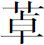
\includegraphics{./images/Image00007.jpg}
  \end{minipage}}\\
  \subfloat[经鞍上池层面]{
  \begin{minipage}[b]{0.7\textwidth}
    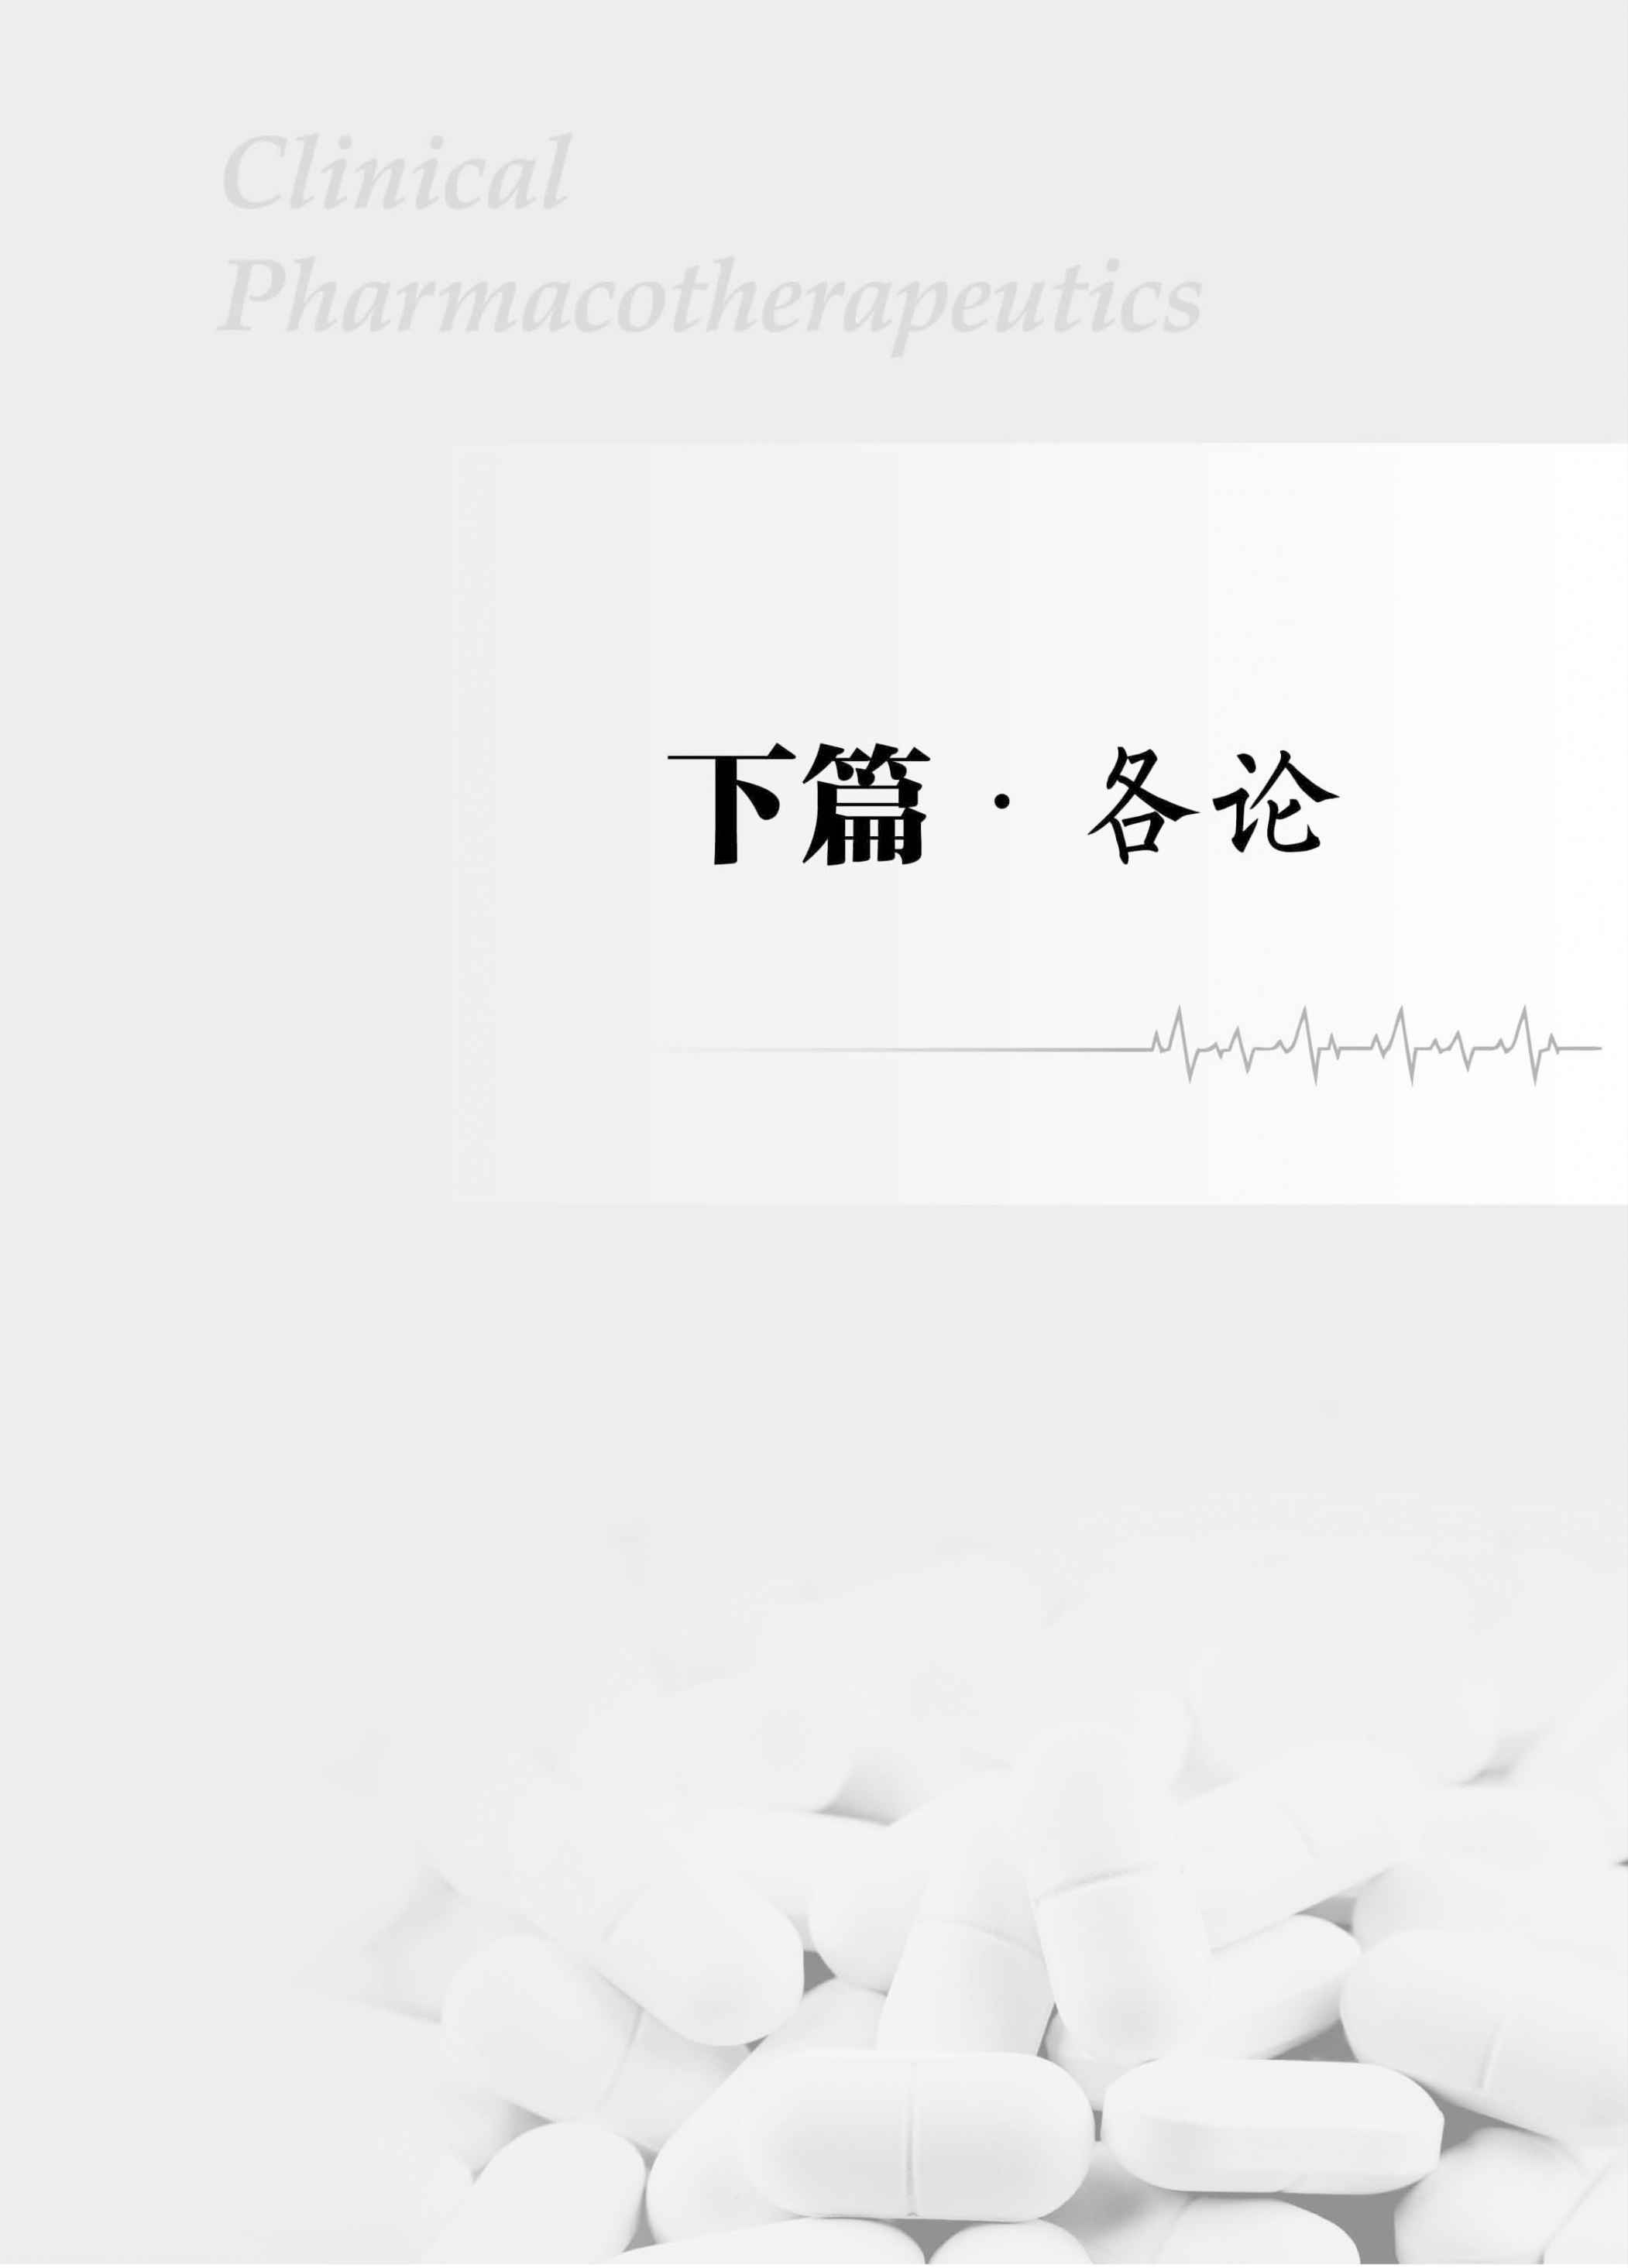
\includegraphics{./images/Image00008.jpg}
  \end{minipage}}\\
  \subfloat[经三脑室下部层面]{
  \begin{minipage}[b]{0.7\textwidth}
    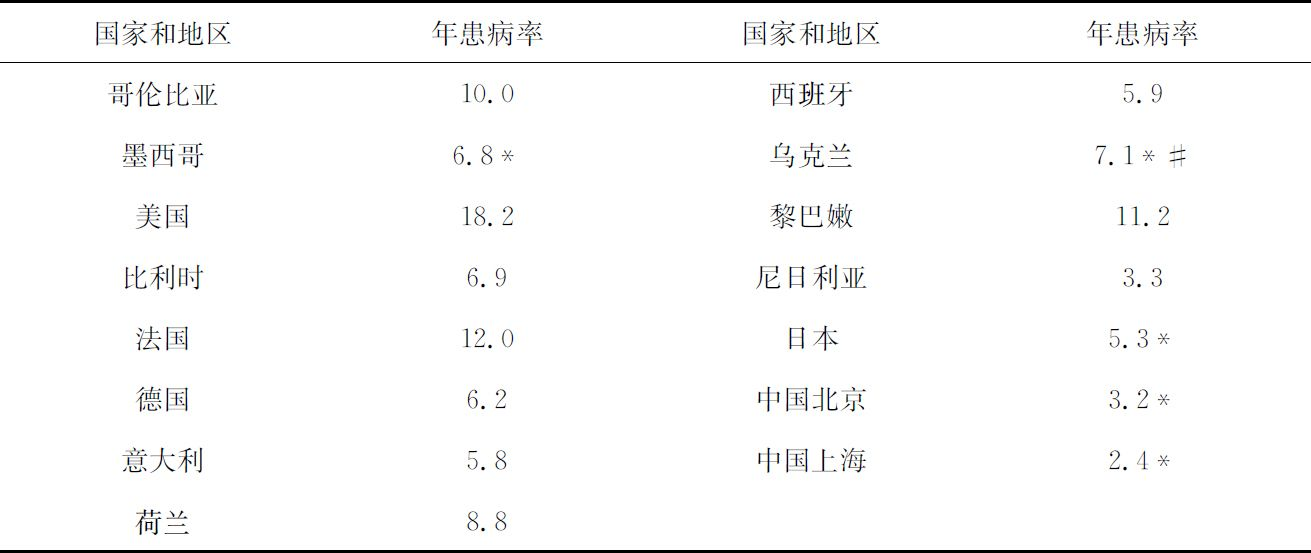
\includegraphics{./images/Image00009.jpg}
  \end{minipage}}
  \caption{}
  \label{fig2-3}
  \end{figure}

  \begin{figure}
    \ContinuedFloat             %%<-- put this in subsequest figures.
    \centering
    \subfloat[经松果体层面]{
      \begin{minipage}[b]{0.7\textwidth}
        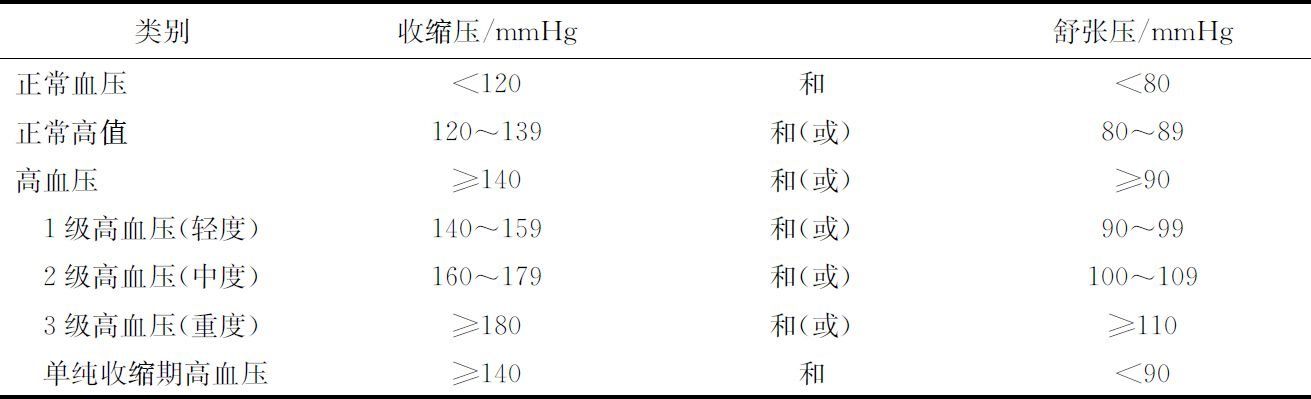
\includegraphics{./images/Image00010.jpg}
      \end{minipage}}\\
      \subfloat[经三脑室上部层面]{
      \begin{minipage}[b]{0.7\textwidth}
        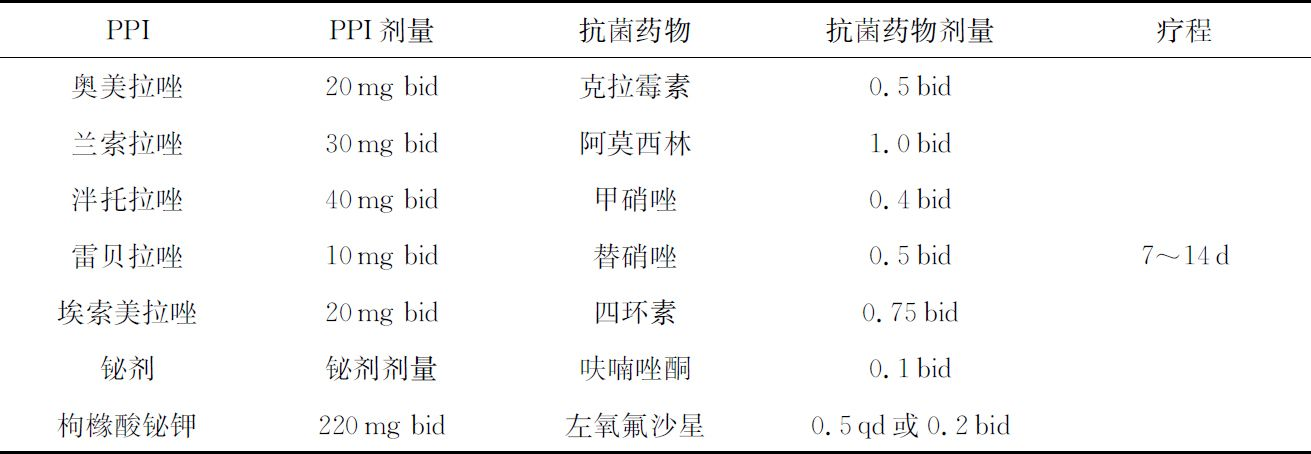
\includegraphics{./images/Image00011.jpg}
      \end{minipage}}\\
      \subfloat[经侧脑室体部层面]{
      \begin{minipage}[b]{0.7\textwidth}
        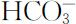
\includegraphics{./images/Image00012.jpg}
      \end{minipage}}
      \caption[]{}
  \end{figure}

  \begin{figure}
    \ContinuedFloat             %%<-- put this in subsequest figures.
    \centering
    \subfloat[经胼胝体体部层面]{
      \begin{minipage}[b]{0.7\textwidth}
        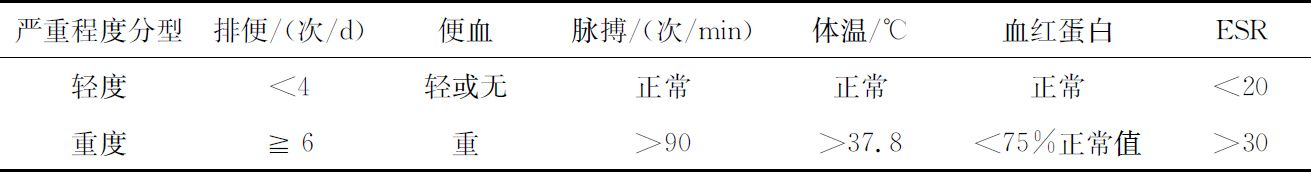
\includegraphics{./images/Image00013.jpg}
      \end{minipage}}\\
      \subfloat[半卵圆中心层面]{
      \begin{minipage}[b]{0.7\textwidth}
        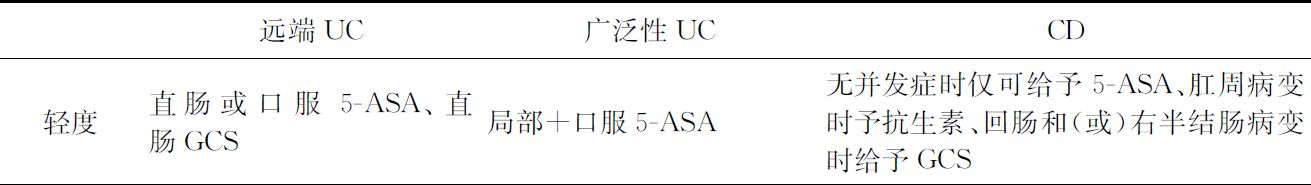
\includegraphics{./images/Image00014.jpg}
      \end{minipage}}\\
      \subfloat[半卵圆中心以上层面]{
      \begin{minipage}[b]{0.7\textwidth}
        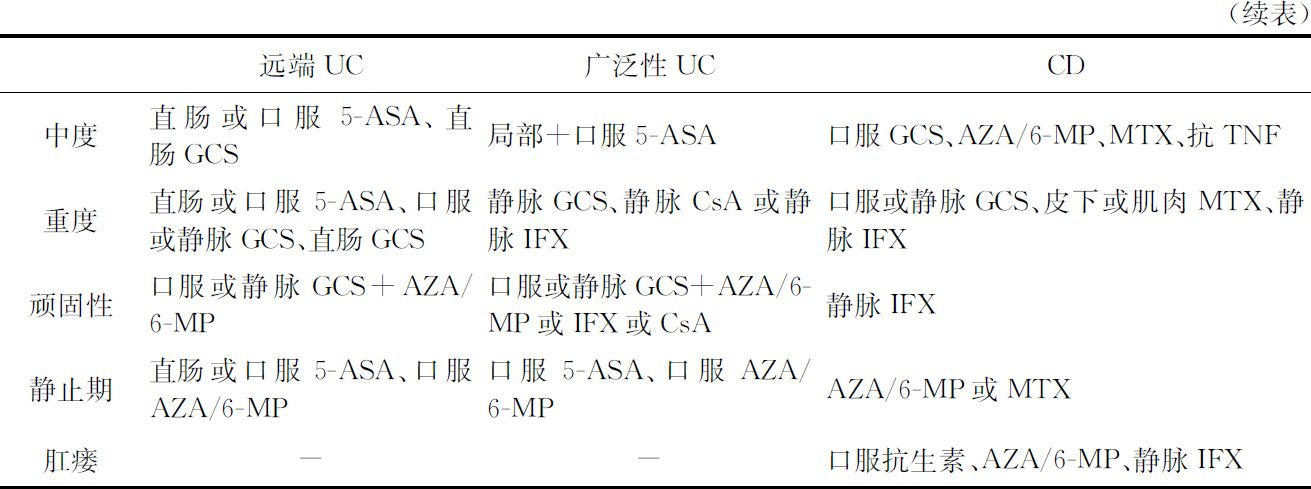
\includegraphics{./images/Image00015.jpg}
      \end{minipage}}\\
      \caption[]{}
  \end{figure}

  \begin{figure}
    \centering
    \subfloat[大脑半球外侧面的主要沟回]{
    \begin{minipage}[b]{0.7\textwidth}
      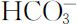
\includegraphics{./images/Image00016.jpg}
    \end{minipage}}\\
    \subfloat[大脑半球内侧面的主要结构]{
    \begin{minipage}[b]{0.7\textwidth}
      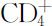
\includegraphics{./images/Image00017.jpg}
    \end{minipage}}\\
    \caption{}
    \label{fig2-4}
    \end{figure}

    \begin{figure}
      \ContinuedFloat             %%<-- put this in subsequest figures.
      \centering
      \subfloat[大脑半球背外侧面功能分区示意图]{
    \begin{minipage}[b]{0.7\textwidth}
      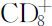
\includegraphics{./images/Image00018.jpg}
    \end{minipage}}\\
    \subfloat[大脑半球内侧面功能分区示意图]{
    \begin{minipage}[b]{0.7\textwidth}
      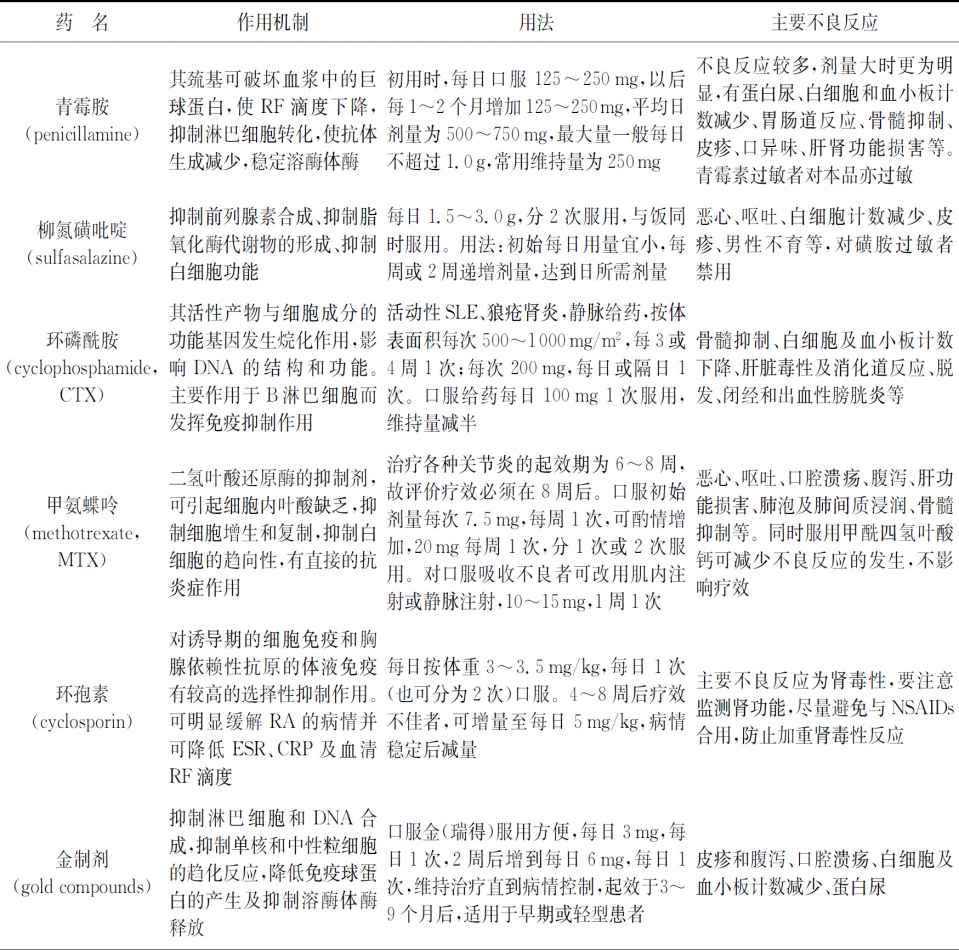
\includegraphics{./images/Image00019.jpg}
    \end{minipage}}\\
        \caption[]{}
    \end{figure}

\section{先天颅脑发育畸形和变异}

\subsection{概述}

所谓畸形是指胚胎期或胎儿期发生的脏器、系统或全身的形态异常或形成异常,不包括出生时的损伤和生后发育成长中产生的障碍。

先天性颅脑发育畸形的发病原因是由于胚胎期神经系统发育异常所致,约40%为遗传因素和子宫内环境的共同影响所致。前者包括染色体变异、显性或隐性遗传;后者包括宫内缺氧、感染等。其余60%病因复杂,机制不详。目前,可分为以下3大类:

1.器官形成障碍:①神经管闭合障碍:以脊髓脊膜膨出最常见,主要包括颅裂畸形(脑膜膨出、脑膨出、无脑畸形)、小脑扁桃体延髓联合畸形(Chiari畸形)、胼胝体发育不全、胼胝体脂肪瘤、先天性四脑室中侧孔闭锁(Dandy-Walker综合征)。②脑裂形成障碍:前脑无裂畸形(单叶、半叶、全叶)、视隔发育不良。③神经元移行异常:又称脑沟及细胞移行障碍,主要包括脑裂畸形、无脑回、灰质异常(巨脑回、多微脑回、灰质异位)。④大小异常:包括脑大、脑小畸形。⑤破坏性病变:包括积水性无脑畸形、脑穿通畸形。

神经管闭合不全是指胚胎期神经沟发育形成神经管的过程中,由于发育障碍而造成神经系统及其周围结构缺陷的一类中枢神经系统先天畸形,可能与孕妇叶酸缺乏有关。除表现出神经症状和体征外,更为常见的是周围组织的异常,包括颅骨、脑膜、椎体及其附件、皮肤和皮下组织(如先天性皮毛窦)等。该类疾病相当常见,其中尤以脊柱的畸形为多,是脑部的10倍或更多。

大脑皮层的神经元来自胚胎时期的脑室壁即神经管上皮。胚胎第6周末神经管经分化形成4个胚胎带,由内向外分别为脑室带、脑室下带、中间带和边缘带。脑室带和脑室下带的细胞具有分化成各类神经元的功能,故又称为生发基质层。胚胎7周时生发基质层的成神经细胞逐渐向外移行,大部分穿过中间带在边缘带内分化成神经元,形成有6层结构的正常脑皮质。26~30周脑回完全形成。神经元移行的过程复杂漫长,此间受到干扰则造成移行障碍。临床均以癫痫、智力障碍为最常见症状。

2.组织发生障碍:总体脑结构正常,但有异常细胞存在并持续分化。①神经皮肤综合征:包括神经纤维瘤病、脑颜面血管瘤病(Sturge-Weber综合征)、结节性硬化、视网膜小脑血管瘤病(又称Von
Hippel-Lindan病)。②血管性病变。③先天性肿瘤。

3.细胞发生障碍:①先天性代谢异常:包括氨基酸尿症、黏多糖沉积病、脂质沉积病等。②脑白质营养不良。③神经元变性。④轴索营养不良。

\subsection{脑膜膨出和脑膜脑膨出}

本病即显性颅裂畸形或称囊性颅裂畸形。临床可见颅外软组织肿物,大多于出生时即可发现。如仅有颅骨缺损,而无内容物自缺损处膨出称为隐性颅裂。

\textbf{【病理】}
颅裂多发生于中线或中线旁(斜坡除外),硬膜常缺如。脑膜(软膜和蛛网膜)或(和)脑突出于脑外,严重时可含部分脑室,可合并其他神经管闭合障碍(如Chiari畸形、胼胝体发育不全)等畸形。

\textbf{【临床表现】}
囊性肿物与头部相连,于出生时即可发现,也可于生后几个月或几年发现。哭闹或咳嗽时肿物增大,张力增加;压迫肿物,则前囟突出;局部可扪及骨缺损的边缘。一般无神经系统症状,也可表现为智力低下、抽搐及脑损害表现。

\textbf{【CT表现】}
软组织疝出的部位可见边缘硬化的颅骨缺损,枕部占70%,顶部占10%~20%,额上部占10%,颅底部占10%。应注意向颅外膨出的软组织,是否含有脑脊液和脑组织;颅底部膨出应注意与鼻息肉或鼻咽部肿瘤相鉴别(图\ref{fig2-5}\footnote{16岁女性,枕骨局限缺损,可见疝出之少量软组织密度灶})。同时,可合并胼胝体缺失、Chiari畸形、灰质异位等畸形。

\begin{figure}[!htbp]
 \centering
 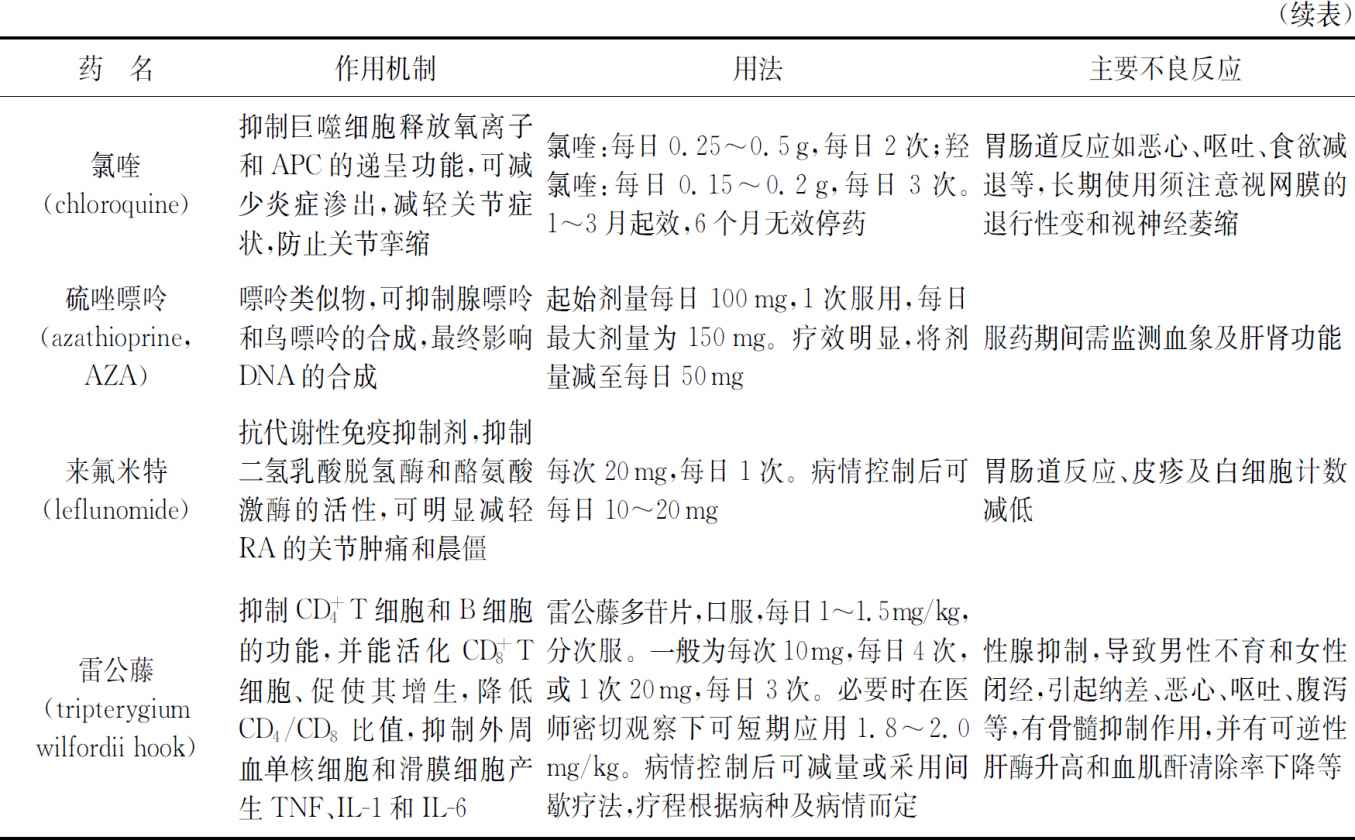
\includegraphics[width=.7\textwidth,height=\textheight,keepaspectratio]{./images/Image00020.jpg}
 \captionsetup{justification=centering}
 \caption{脑膜脑膨出}
 \label{fig2-5}
  \end{figure} 

\subsection{小脑扁桃体延髓联合畸形}

本病又称Chiari畸形,为后脑先天性发育异常。扁桃体过长、变形,经枕大孔疝入上段颈椎管,延髓和第四脑室可同时向下延伸。常伴脊髓空洞症、脊髓纵裂、脑积水和颅颈部畸形等。

\textbf{【病理】} 可分为以下4型。

Ⅰ型:多见。最可能的发病机制是胚胎枕节发育不良导致后颅窝狭小,难以容纳正常发育的后脑,使小脑扁桃体下疝。小脑扁桃体与小脑下部疝入颈椎管上端,无延髓移位。一般认为小脑扁桃体下端低于枕大孔≥5mm为下疝,<3mm为正常,二者之间临床意义不确定。通常不伴其他脑畸形,临床可无症状,或有轻度运动障碍和小脑症状。

Ⅱ型:最常见。小脑扁桃体和蚓部同时疝出枕大孔,脑桥下部及延髓下移,第四脑室延长。几乎总是伴有某种神经管闭合不全如脑膜膨出、脊髓脊膜膨出(腰骶部多见)、脑积水和脊髓空洞症。常有上述Ⅰ型症状。

Ⅲ型:十分罕见。为Ⅱ型伴有低枕部或高颈部脑膜脑膨出,临床症状较Ⅱ型更严重。

Ⅳ型:非常罕见。伴有严重的小脑发育不良,结构独特,可能不单独存在。该型归为小脑发育不良可能更合适。

\textbf{【临床表现】}
本病可无症状,尤其畸形轻者可无,也可直到成年甚至50~60岁始有症状。神经损害症状主要是颅神经和颈神经受损、延髓和上颈髓受压,可有小脑症状、颅内高压及脊髓空洞症表现。

\textbf{【CT表现】}
CT可显示下列特征:①小脑扁桃体、小脑蚓部及小脑、脑干和第四脑室下移;②脑积水;③大脑镰和天幕发育不良;④部分脑组织过度增生或脑发育异常导致脑室系统畸形;⑤后颅窝内容物的挤压引起的颅骨和蛛网膜下腔的改变。但只有通过脑池造影CT扫描或MR显示扁桃体下移、其下端变尖才能明确诊断。

\subsection{侧孔先天性闭锁}

本病又称Dandy-Walker综合征,第四脑室正中孔、外侧孔闭锁为发病主要原因。

\textbf{【病理】}
此病是一组先天性后脑发育畸形,包括脑积水、小脑发育障碍(小脑蚓部不发育或发育不全,约25%蚓部缺如)和与第四脑室相通的巨大后颅窝囊肿。囊肿大小变化很大,囊壁由下髓帆组成,包括室管膜、胶质、小脑组织、软脑膜和蛛网膜等,囊壁可钙化,可合并大脑发育异常。

\textbf{【临床表现】}
男女发病率相近。大多于2岁前产生症状,常因运动发育迟缓而就诊。部分因颅内高压或小脑症状而就诊,头颅明显增大。

\textbf{【CT表现】}
在出生时脑积水是不常见的,75%在生后3个月出现。典型者小脑蚓部体积变小或缺如,小脑半球分离;巨大的后颅窝“囊肿”与扩大的第四脑室相通。脑干前移,桥前池、桥小脑角池消失,后颅窝扩大,枕骨变薄,天幕上移。可合并胼胝体发育不良、多微脑回、灰质异位、枕部脑膨出等。

\textbf{【鉴别诊断】}
①后颅窝巨大蛛网膜囊肿:第四脑室与囊肿不相通,而是受压前移,必要时通过脑池造影CT鉴别。②巨大枕大池:第四脑室无受压,无蚓部发育不全、无后颅窝扩大等,但与下蚓部几乎完整的Dandy-Walker畸形不易鉴别。上述两者均可偶有轻度脑积水,但小脑发育基本正常。

\subsection{Joubert综合征}

\textbf{【病理】}
病理特征是小脑蚓部不发育或发育不全而形成异常的“中线裂”,还有小脑齿状核的变形、下橄榄核和旁橄榄核的发育不良、背侧柱核的异常以及锥体交叉缺如。

\textbf{【临床表现】}
男性多见,有发作性呼吸过度和(或)呼吸暂停、眼球活动异常(眼球震颤、斜视等)和儿童期发育迟缓。还可伴有其他异常如小头畸形、面部畸形、胼胝体发育不全、多指畸形和先心病等。

\textbf{【CT表现】}
在桥脑和中脑连接水平,第四脑室呈“蝙蝠翼状”。于第四脑室底部紧贴小脑半球中线处可见小脑半球间形成的切迹即“中线裂”。小脑上脚增粗,由于交叉的缺乏而向外分开,并导致中脑背侧局部缺失,形成所谓的“磨牙征”。第四脑室中部呈倒立三角形状,与不连接的小脑半球间的脑脊液间隙相连形成“酒杯状”表现,无后颅窝囊肿和脑积水。

\subsection{胼胝体发育不全}

\textbf{【病因病理】}
胼胝体在妊娠12~20周时形成。本畸形偶然发病,病因一般不明,多为先天性。在某些病例中,母体的血管性、外伤性、中毒性或感染性损伤为致病因素。产期缺血缺氧性损害也可引起获得性胼胝体发育不全。本病可为全部或部分缺如,常伴发其他畸形(最高达50%),如前脑无裂畸形、多微脑回、厚脑回、灰质异位、脑小畸形、视隔发育不良、胼胝体脂肪瘤或纵裂池蛛网膜囊肿等。

\textbf{【临床表现】}
临床症状各不相同,视伴发的其他神经系统畸形而定。许多患者可无症状或仅有轻度视觉障碍;或有交叉触觉定位障碍而智力正常;严重者可有癫痫和智力不全。

\textbf{【CT表现】}
由于胼胝体完全或部分缺如而表现不一。可见纵裂池前部明显向后伸展,靠近第三脑室前壁。侧脑室额角和体部间距增大,而且两侧脑室平行分离,并可见其内壁呈弓形外突,冠扫额角呈“八”字形分离。枕角不对称性扩大(憩室),第三脑室轻度扩大并上移。正常时,两侧脑室的脉络丛常在室间孔间会聚,并形成45\textsuperscript{o}
~70\textsuperscript{o} 夹角,本病此夹角多<35\textsuperscript{o}
~40\textsuperscript{o}
(图\ref{fig2-6}\footnote{A~D为同一患者,可见纵裂池前部明显向后伸展,靠近第三脑室前壁;第三脑室轻度扩大并上移;侧脑室额角和体部间距增大,两侧脑室平行分离}),有时可见半球间裂(纵裂池)的蛛网膜囊肿等畸形。本病应注意与脑室周围白质软化症(PVL)相鉴别。



\begin{figure}[!htbp]
 \centering
 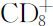
\includegraphics[width=\textwidth,height=\textheight,keepaspectratio]{./images/Image00021.jpg}
 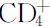
\includegraphics[width=\textwidth,height=\textheight,keepaspectratio]{./images/Image00022.jpg}
 \captionsetup{justification=centering}
 \caption{胼胝体发育不全}
 \label{fig2-6}
  \end{figure} 


\subsection{前脑无裂畸形}

本病又称全前脑畸形,是胚胎发育过程中由前脑发育障碍引起的一组复杂的颅脑与面部畸形。

\textbf{【病因病理】}
其病因不明,部分为常染色显性和隐性遗传。大脑不能分裂成两侧大脑半球,有时也不能在横向上分裂成端脑和间脑,可分为无脑叶型、半脑叶型、脑叶型3种类型,代表了畸形的不同程度。

\textbf{【临床表现】}
男女发病相近,因婴儿多数死于流产或出生后不久,故临床少见。脑叶型可活到成年,并有运动迟缓、智力低下等神经精神症状。

\textbf{【CT表现】} 3种类型分别表现如下。

1.无脑叶型:又称全前脑无裂畸形。脑呈小圆球形,丘脑融合,中央单脑室,第三脑室成为扩大脑室的一部分。正常中线结构如透明隔、大脑镰、胼胝体和纵裂均缺失,50%以上有多处面颅畸形。

2.半脑叶型:中央单脑室较小,初步形成了额、枕角,胼胝体、大脑镰、透明隔仍缺如。大脑半球前部仍保持融合,但后部半球间裂已形成。丘脑往往部分分离,故第三脑室是小的,面部畸形不重。

3.脑叶型:CT表现比前两者轻微。前部半球间裂较浅,仍存在融合表现。脑室系统形态良好,透明隔缺如。脑镰和胼胝体至少部分形成,丘脑无融合。

此外,少数病例额部和枕部半球间裂均存在,融合发生于半球额后顶区域,属半脑叶型,CT诊断困难。

\subsection{视隔发育不良}

本病罕见,主要是透明隔发育不全,常见于先天性垂体性侏儒,可能是脑叶型前脑无裂畸形的轻度形式。

\textbf{【病理】}
透明隔发育不全,有原始的视泡及视交叉、视神经,漏斗发育不全而使视神经孔狭小。

\textbf{【临床表现】}
眼部症状包括眼球震颤和视敏度下降,但可有正常视力。约2/3有下丘脑-垂体功能障碍而出现尿崩、生长发育障碍。

\textbf{【CT表现】}
透明隔缺如,额角在横断面呈倒三角形或盒状。严重者可见视神经、视交叉细小,视神经管小和视交叉位置异常,视交叉和下丘脑发育不全使鞍上池扩大。

\subsection{透明隔疾病}

透明隔是一厚约1.5~3.0mm的双层半透明膜,上起胼胝体的体部、膝部和嘴部,向下延伸至穹隆的表面,前后伸延从终板、胼胝体的嘴至胼胝体的压部。它含有一定数量的胶质细胞、散在的神经元和神经纤维。这些神经纤维构成了海马和下丘脑之间的重要联系,且是中继下丘脑到海马、杏仁核、缰核和脑干网状结构的内脏信息的相关中心及边缘系统到脑干网状结构的重要环路。所以,它参与意识、睡眠以及环境作用所表现出来的情绪反应,例如饮食、性活动等,并有助于精神活动的自我平衡。

透明隔疾病有:①透明隔间腔:即第五脑室。②透明隔缺如:原发或继发。③透明隔囊肿:与第五脑室并无严格界限,表现囊壁向两侧突出而不是平行,宽达10mm以上,并可引起室间孔狭窄导致脑积水,邻近神经组织受压而引起神经功能障碍。当宽径<5mm时,则不引起症状(图\ref{fig2-7})。④肿瘤:罕见,如星形细胞瘤、少突胶质细胞瘤、室管膜瘤和成星形细胞瘤,近来亦有亚室管膜瘤、局限性脂肪瘤的报道。⑤血管瘤。⑥钙化。⑦移位。⑧萎缩。

\begin{figure}[!htbp]
 \centering
 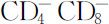
\includegraphics[width=.7\textwidth,height=\textheight,keepaspectratio]{./images/Image00023.jpg}
 \captionsetup{justification=centering}
 \caption{透明隔囊肿\\{\small 透明隔区囊状水样密度灶,囊壁向两侧突出,宽达12mm}}
 \label{fig2-7}
  \end{figure} 



\subsection{侧脑室黏合}

侧脑室不对称在正常人中常见,部分原因是侧脑室黏合,侧脑室黏合是正常变异。

\textbf{【病理】}
本症是在生长发育过程中侧脑室内面部分融合,造成侧脑室不对称、变形。发生在胎儿期4~6周,此时脑白质发育迅速,白质膨大可使邻近的室管膜表面挤压在一起。黏合多发生在额角上侧面及体部,单侧或双侧性。

\textbf{【CT表现】}
侧脑室黏合可以是单侧性或双侧性,或与透明隔间腔同时存在。额角的前部融合,致额角前部消失,额角变短,两壁夹角为锐角,使两壁相交处圆钝的正常表现消失,透明间隔居中。额角中部的两壁尖角状突起,中部间隙消失或接近消失,透明隔居中。透明隔移向一侧,偏移程度从轻度到非常明显,致同侧侧脑室体部变小,对侧相对增大。透明隔的移位必然伴有体部变小侧的额角变窄、变形,但透明隔始终呈直线状走行。双侧基底节区形态结构对称,脑室、脑实质内无异常,增强扫描无异常强化。

\subsection{脑裂畸形}

\textbf{【病因病理】}
有学者认为,妊娠第2个月出现的病理干扰可造成脑壁某部位生发基质层不能正常发育,致使神经元移行不能发生或过早停下来而导致脑裂畸形。其主要病理改变为大脑半球内有自脑表面向内延伸达室管膜下的横行裂隙,邻近皮层卷入衬于裂隙两侧,其表面的软脑膜与室管膜融合形成软脑膜-室管膜缝。脑裂畸形可分为闭合型和分离型两型,常合并透明隔缺如、胼胝体发育不良及其他神经元移行异常等畸形。

\textbf{【临床表现】} 主要有癫痫、智力低下和运动功能障碍。

\textbf{【CT表现】}
大脑半球表面有单侧或两侧的裂隙,从脑表面延伸到室管膜下区。脑皮质沿裂隙内折,居裂隙两侧,多位于中央前后回附近。根据其表现可分为两型:①Ⅰ型:即融合型(或称闭唇型)脑裂畸形,裂隙关闭不与侧脑室相通,但脑室壁可有憩室样突起(图\ref{fig2-8});②Ⅱ型:即分离型(或称开唇型)脑裂畸形,特点为内折的皮质分离,形成较大裂隙并多与侧脑室相通,且脑室壁在内压作用下外突,形成憩室。

\textbf{【鉴别诊断】}
①脑穿通畸形:为大脑成形后的损害(坏死腔),多呈圆形,无脑皮质沿囊肿壁内折为鉴别要点。有时鉴别困难,但穿通畸形的两缘向病灶外方突出,而分离型脑裂畸形两缘向内突出有助于鉴别。②孤立性灰质异位:当融合型裂隙不明显时应注意与其鉴别。脑裂畸形皮质柱内端相邻的侧脑室外壁常有憩室状突起,外端脑表面有楔形凹痕,可与其相鉴别。

\subsection{多微脑回畸形和鹅卵石样脑回畸形}

\subsubsection{无脑回}

大脑皮质表面光滑、无沟回,故又称光滑脑。灰质增厚,白质变薄,灰白质正常手指样交界消失,也可与巨脑回相伴发。

\subsubsection{巨脑回}

局限性或弥漫性脑回异常增宽,皱褶减少,表现为宽、平、厚的脑回,灰白质正常手指样交界亦可消失(图\ref{fig2-8},图\ref{fig2-9})。

\begin{figure}[!htbp]
 {\centering
 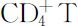
\includegraphics[width=.7\textwidth,height=\textheight,keepaspectratio]{./images/Image00024.jpg}
 \captionsetup{justification=centering}
 \caption{脑裂畸形、双侧额叶巨脑回\\{\small  A、B为同一患者,大脑半球表面两侧均有裂隙,脑皮质沿裂隙内折,位于裂隙两侧,裂隙关闭不与侧脑室相通,灰质相应内移,双侧额叶巨脑回}}
 \label{fig2-8}}
  \end{figure} 



\begin{figure}[!htbp]
 {\centering
 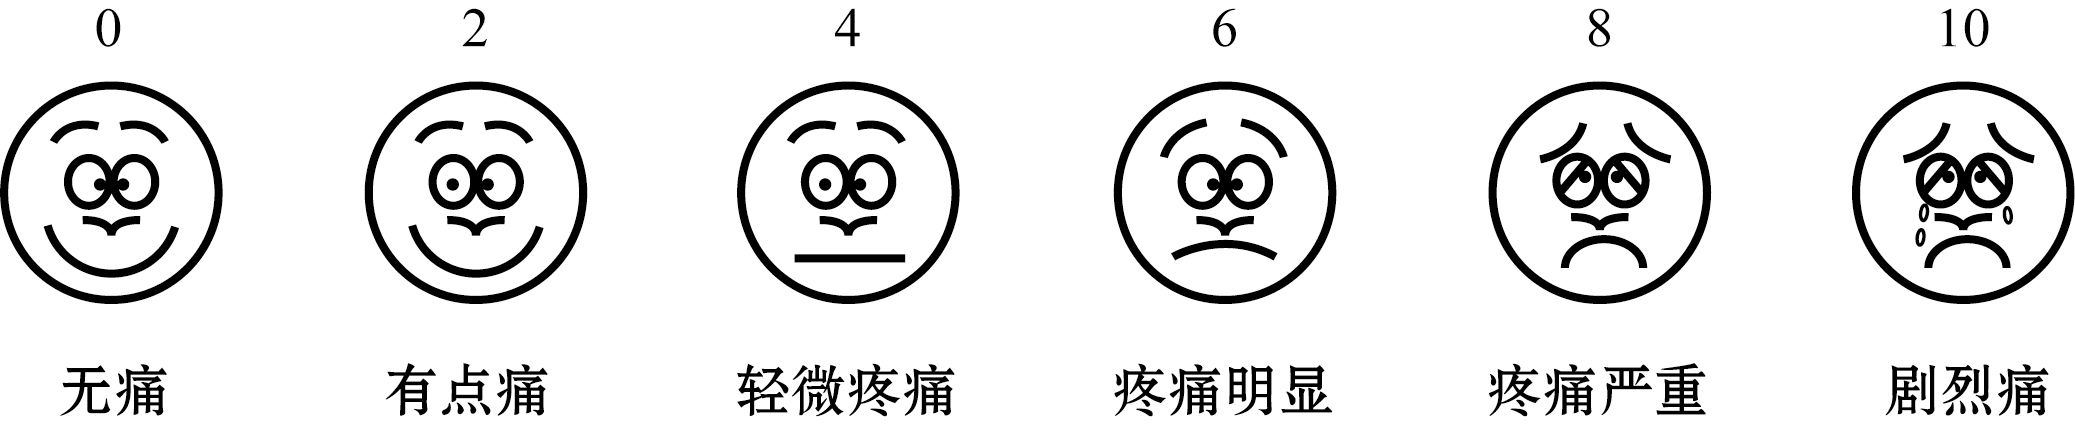
\includegraphics[width=.7\textwidth,height=\textheight,keepaspectratio]{./images/Image00025.jpg}
 \captionsetup{justification=centering}
 \caption{巨脑回}
 \label{fig2-9}}

 右侧额、顶叶脑回弥漫性异常增宽,皱褶减少
  \end{figure} 



\subsubsection{多微脑回畸形}

亦称多小脑回畸形(但该名称易与小脑病变混淆),脑回小且数目增多。

\subsubsection{鹅卵石样脑回畸形}

为复杂的脑畸形,包括鹅卵石样皮质、白质异常、脑室扩大,及脑干、小脑变小并伴有小脑的多微脑回。皮质的异常为无脑回、巨脑回和多微脑回的混合。

\subsection{灰质异位}

本病为灰质在异常部位的聚集。

\textbf{【病因病理】}
原因不明,可能与遗传性、血管性、感染性、环境因素(中毒、辐射、胎儿酒精综合征等)等有关。病理上根据异位灰质灶是否与室管膜相连分为室管膜下型和非室管膜下型,根据病变范围又可分为局灶性和弥漫性。弥漫性90%为女性,往往具有家族史。本病还可伴有其他畸形。

\textbf{【临床表现】}
单纯的灰质异位预后好,可无症状或仅有癫痫。病灶较大或同时伴有其他畸形可表现为中度或严重发育延迟、偏瘫伴癫痫。

\textbf{【CT表现】}
白质内有与灰质密度相等的异常影,增强扫描密度与灰质一致。本病有多种分型方法,通常可分为以下3型。①结节型:呈结节状分布于侧脑室旁,并可突向脑室。②板层型:不规则分布于白质内。③带状型:呈带状分布于白质或皮层下(是最严重的类型,常伴有难治性癫痫,预后相对差)。前两型可单发或多发、单侧或双侧,灰质结节直径1~30mm,无水肿和占位效应。带状型多分布对称,且表面脑回多正常,故较难分辨,易漏诊。

\subsection{脑大畸形}

本病又称头大畸形、巨脑症,为先天性大脑皮质增厚及神经胶质细胞增生。

\textbf{【病因病理】}
本病病因不明,可与遗传因素有关。有学者认为包括体积过大和质量过重两种情况,并将它分为解剖型和代谢型巨脑症。解剖型指细胞体积或数目大于正常,可伴软骨发育不全、神经纤维瘤病、结节性硬化和Chiari畸形等。代谢型是指异常代谢产物积蓄致脑细胞增大,部分伴白质发育不良。本病出生时脑重即可达1600g,或生后头颅迅速增大,皮质和髓质均增厚,可有髓鞘形成不良,无脑积水。

\textbf{【临床表现】}
儿童期发病,常有癫痫和智能低下。头颅周径增大,似先天性脑积水,但无眼球下斜征象(落日征),常有视、听力障碍。

\textbf{【CT表现】}
头颅和颅腔明显增大,大脑皮质增厚,但脑组织密度正常。脑室正常或轻度扩大,脑沟、池正常,中线结构居中。前囟较大、闭合延迟,颅板较薄。

\textbf{【鉴别诊断】}
应注意与继发性巨脑症(如较弥漫的肿瘤、结节性硬化、海绵状硬化及脑积水)、单侧巨脑畸形相鉴别。

\subsection{脑小畸形}

本病又称小脑症、小头畸形或脑小症,发病率为2.5/10万。

\textbf{【病因病理】}
病因不明,可包括先天性遗传因素和胎儿期、新生儿期的各种致病因素如感染、出血、缺氧、产伤等。病理表现为脑小,重量为正常的1/4~1/3,并且脑回结构简单,皮质发育不全,神经元数目减少、排列不整齐,颅骨和颅腔发育小,可合并其他脑发育畸形。

\textbf{【临床表现】}
常表现智能低下甚至呈白痴,也可合并癫痫、运动功能障碍等,出生时头小、外形特殊。

\textbf{【CT表现】}
轻度者可无阳性表现,病变明显时脑室系统和蛛网膜下腔可扩大,皮质光滑,缺乏脑沟、回。严重者可合并胼胝体发育不全、透明隔发育异常、穿通畸形等。颅腔缩小以额部明显,颅板较厚,板障增宽,内板平坦光滑。

\textbf{【鉴别诊断】}
狭颅畸形是颅缝过早闭合限制了脑的发育所致。颅腔常有变形,颅骨脑回压迹增多,且脑室、脑沟、脑池及脑实质常无明显异常,不难与脑小畸形鉴别。此外,一侧大脑半球发育不全与脑小畸形病因病理一样,临床和CT表现相近,不难诊断和鉴别。

\subsection{积水型无脑畸形}

本病是一组少见的先天性前脑畸形,见于婴幼儿,发生率新生儿中占0.2%左右。

\textbf{【病因病理】}
可能与胚胎期脑供血障碍有关,也有人认为是全脑穿通畸形。主要病理改变为双侧大脑半球的额、顶、颞叶完全或大部分缺如,由充满脑脊液的囊性区域取代,其内衬由软脑膜构成(不含室管膜)。基底节、丘脑、中脑可部分或大部分破坏,小脑、桥脑、延髓可发育正常或畸形,脑室系统偶可保存完好,脑膜正常存在,颅骨颅腔大小形态正常或增大。

\textbf{【临床表现】}
头围逐渐增大,多智力低下,可有眼球不规则运动、眼落日征,以及肌张力高、腱反射亢进、抽搐或惊厥、运动机能障碍等。

\textbf{【CT表现】}
幕上双侧大脑半球、脑室大部分缺失,整个颅腔大部分呈脑脊液密度。仅于脑底部见残存的部分枕、额或(和)颞叶组织,基底节、丘脑部分存在,大脑镰完整存在。幕下结构正常,但脑干可略变细。

\textbf{【鉴别诊断】}
有学者把极其严重的双侧性开唇型脑裂畸形归类于积水性无脑畸形中,影像学二者难以鉴别,但后者还能识别脑室轮廓,特别是前角的下部和后角。还应注意与无脑叶型前脑无裂畸形、穿通畸形、巨大蛛网膜囊肿及重度脑积水鉴别。

\subsection{脑穿通畸形}

本病是在脑组织分化发育充分之后,由于各种原因造成的脑组织破坏缺损,并与蛛网膜下腔或脑室相通。

\textbf{【病因病理】}
有先天性和获得性之分。先天性病因不明,可能与胎儿期血管闭塞或发育畸形有关;获得性是由于外伤、感染、缺氧、血管疾病引起正常脑组织坏死液化。缺损边缘为胶质瘢痕,不含神经细胞。

\textbf{【临床表现】} 依病变范围而定,可表现运动障碍、癫痫等。

\textbf{【CT表现】}
脑实质内巨大的脑脊液密度样囊肿,界限清楚,增强扫描无强化。与脑室或(和)蛛网膜下腔相通是诊断的关键,同侧侧脑室一般相应扩大。

\subsection{先天性中脑导水管狭窄}

本病亦属脑的发育畸形。

\textbf{【病理】}
狭窄多位于导水管口以下3~4mm处。狭窄的形态多样,可呈线状、鸟嘴状、漏斗状、隔膜状或分叉状,狭窄以上脑室积水。

\textbf{【临床表现】} 临床症状常开始于幼儿,呈慢性脑积水表现。

\textbf{【CT表现】}
侧脑室及第三脑室对称性扩大,第四脑室正常或略小。侧脑室周围有带状低密度区,代表阻塞性脑积水的典型表现。重度积水患者,可表现幕上大脑半球区为水样低密度,额、顶、颞叶脑实质几乎消失或残留极少,部分枕叶、基底核和丘脑保存,小脑和脑干发育一般正常,第四脑室位置、形态正常,可见正常大脑镰结构(图\ref{fig2-10}),MR可显示狭窄的形态。

\begin{figure}[!htbp]
 {\centering
 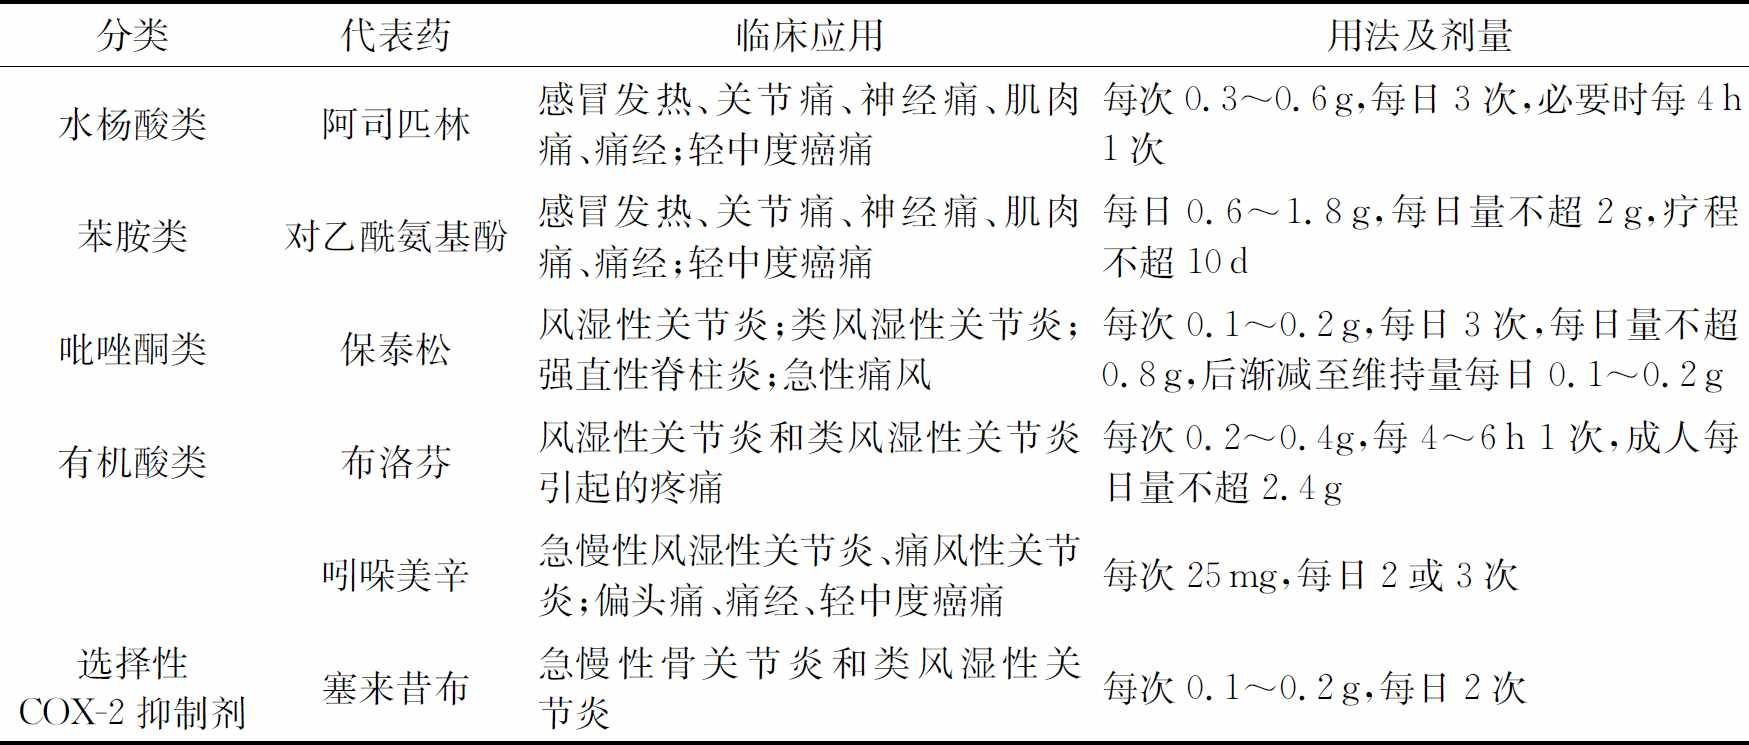
\includegraphics[width=.7\textwidth,height=\textheight,keepaspectratio]{./images/Image00026.jpg}
 \captionsetup{justification=centering}
 \caption{先天性中脑导水管狭窄\\{\small  A、B为同一患者,可见第三脑室、侧脑室积水扩张,额、顶、颞叶脑实质部分残留,枕叶、部分基底核和丘脑保存,小脑和脑干发育正常,第四脑室正常}}
 \label{fig2-10}}
  \end{figure} 



\textbf{【鉴别诊断】}
应注意与松果体区和中脑肿瘤压迫所致的导水管狭窄相鉴别,但肿瘤有占位表现且导水管有移位。炎性粘连所致的导水管狭窄与本病不易鉴别。此外,积水性无脑畸形大脑结构几乎完全消失、脑室基本无残留,枕叶一般相对完整,可予鉴别。

\subsection{结节性硬化症}

本病又称为Bourneville病,是一种较少见的常染色体显性遗传病,发病率约为1/50000~2/10000。

\textbf{【病理】}
病理特征为皮质结节、白质内异位细胞团和脑室内的小结节。结节可发生于皮质、室管膜下,皮质结节最常位于额叶,其次枕叶,偶见于基底节、丘脑、小脑和脑干。皮质结节内含有细胶原纤维、奇异的胶质细胞或不典型的神经元,多数有钙化。脑白质内异位细胞团也是由胶质细胞和神经节细胞组成。室管膜下结节最易钙化,易伴发室管膜下巨细胞型星形细胞瘤,也可伴有视网膜的错构瘤及其他内脏肿瘤。皮质腺瘤由皮质腺、结缔组织和血管组成,但国外有学者认为面部多发的不是皮脂腺瘤,无皮脂腺样结构,而是血管纤维瘤。

\textbf{【临床表现】}
典型的三联征为:①皮质腺瘤占90%;②癫痫发作;③智力低下。但三者不一定同时出现。皮质腺瘤主要位于面颊、鼻、额或两耳处,为对称散发、针头大小、黄红色透亮的坚硬蜡状丘疹。本病还可有眼、心、肾、肺、骨骼病变。

\textbf{【CT表现】}
有以下几方面:①皮质结节:可见脑回扩大、增宽,结节呈低密度,周围为等密度厚皮质围绕。一般无强化,故有人称为空心型病灶。此外,还可呈“H”型皮质结节(低密度病灶中间有一等密度横道)和高密度团块。②室管膜下结节:位于脑室边缘,50%以上双侧对称多发,结节大小不等,部分钙化,未钙化部分强化著(图\ref{fig2-11})。③室管膜下区星形细胞瘤:常位于室间孔附近。④脑白质内异位的细胞丛:皮髓交界区或更广泛的白质内见一些更低密度区。⑤其他:可有脑沟增宽等脑萎缩表现;阻塞室间孔可有脑积水表现。

\begin{figure}[!htbp]
 \centering
 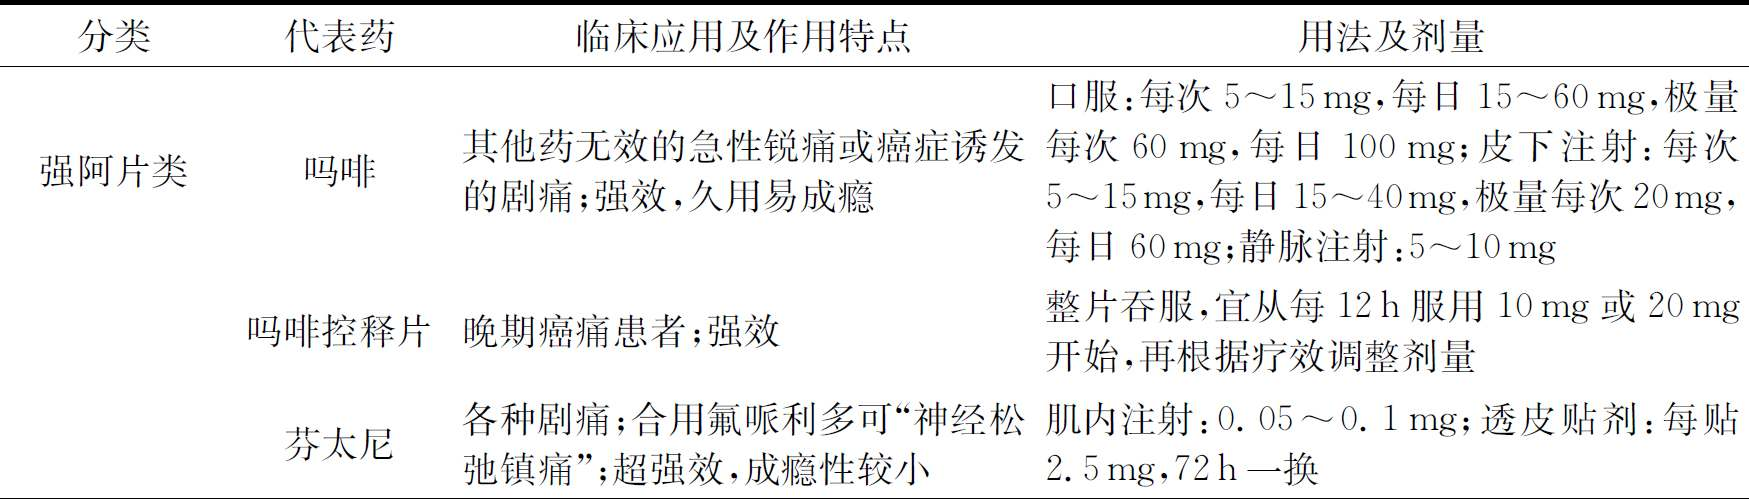
\includegraphics[width=.7\textwidth,height=\textheight,keepaspectratio]{./images/Image00027.jpg}
 \captionsetup{justification=centering}
 \caption{结节性硬化症\\ {\small 左右侧侧脑室边缘可见多个钙化结节,大小不等;右侧额叶有局限性萎缩表现}}
 \label{fig2-11}
  \end{figure} 



\subsection{脑颜面血管瘤病}

本病又称Sturge-Weber综合征或软脑膜血管瘤病。

\textbf{【病因病理】}
此病多为散发,很少有家族遗传史,偶为常染色体显性遗传。病变的分布特点为面部三叉神经分布区皮肤毛细血管瘤和同侧颅内软脑膜血管瘤,病侧大脑发育不良或萎缩。由于软脑膜血管瘤长期压迫或继发性脑缺血可引起皮质梗死,神经节细胞减少、变性,神经胶质增生伴皮质钙化,30%可发生青光眼与脉络膜血管瘤。

\textbf{【临床表现】}
癫痫、痴呆、智力低下,轻偏瘫、偏盲,先天性青光眼、牛眼症(先天性白瞳症)等,还可合并阴睾、脊柱裂等。面部分布葡萄酒色的血管痣,称作火焰痣或葡萄酒斑,出生时即可存在,主要分布在一侧三叉神经分布区,一般同颅内软脑膜血管瘤位于同一侧,但少数也可位于双侧或对侧面部。此外,约5%~15%的患者无面部血管痣。

\textbf{【CT表现】}
患侧皮层曲线状或脑回状钙化为本病特征(图\ref{fig2-12})。患侧大脑皮质萎缩伴脑沟裂、脑池增宽增深及同侧脑室扩张,钙化周围可见梗死灶,偶见出血灶。同侧脑室脉络丛有时增大,颅盖骨板障可增厚。增强扫描钙化灶周围及钙化区可明显强化;增大的脉络丛(亦属血管瘤)有明显强化。在发现脑实质内的缺血缺氧、胶质增生和脱髓鞘改变方面CT不及MR。

\begin{figure}[!htbp]
 \centering
 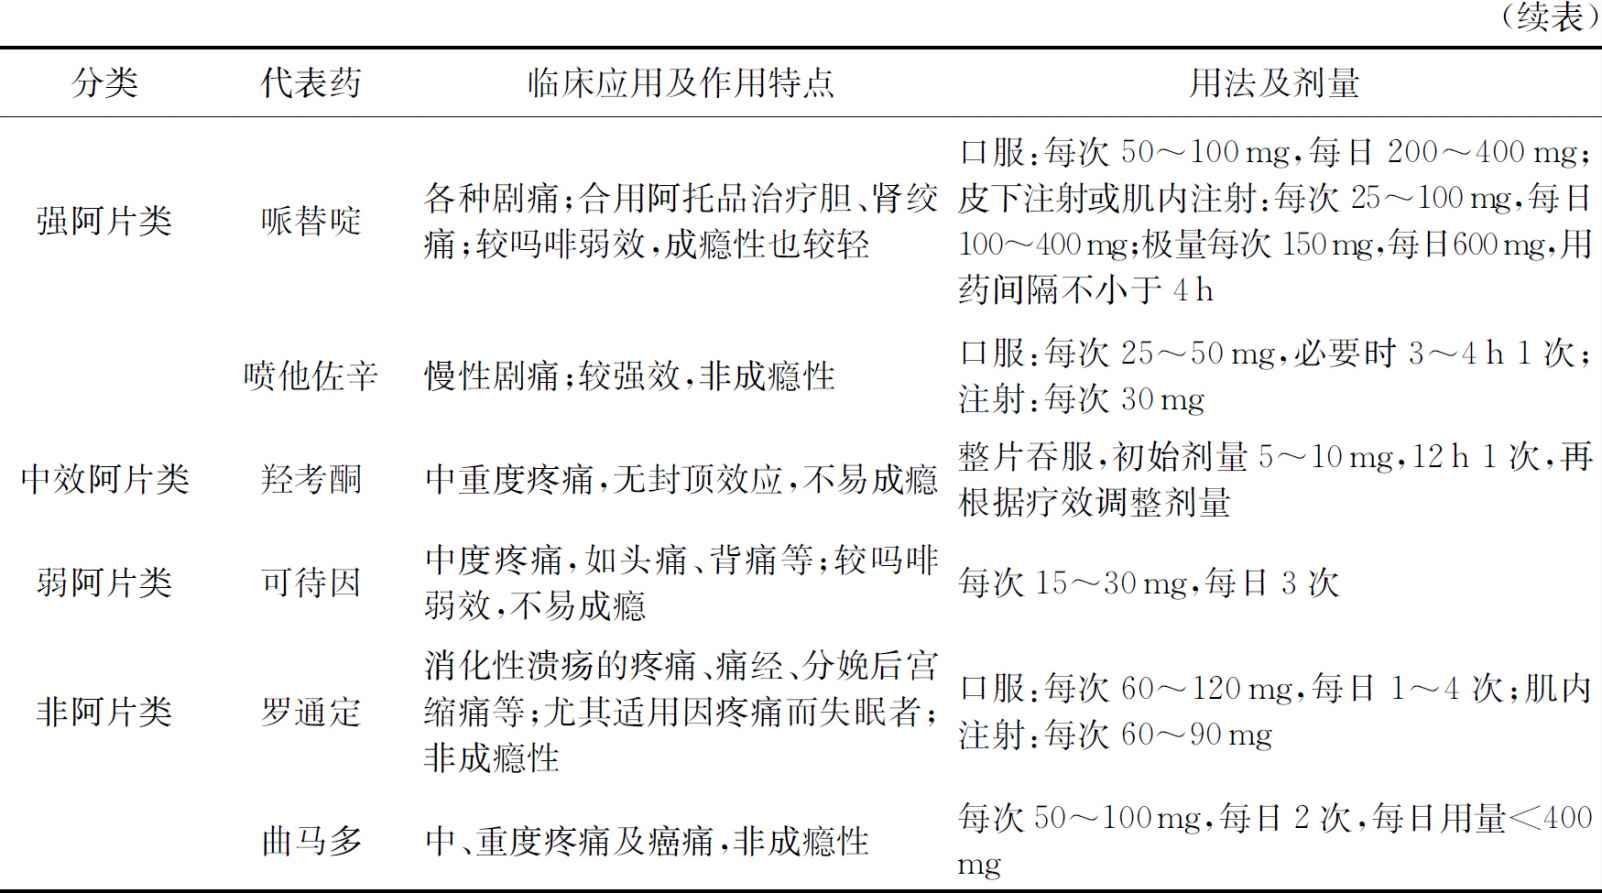
\includegraphics[width=.7\textwidth,height=\textheight,keepaspectratio]{./images/Image00028.jpg}
 \captionsetup{justification=centering}
 \caption{Sturge-Weber综合征\\{\small 右侧额叶皮层曲线状钙化,局部脑沟增宽增深}}
 \label{fig2-12}
  \end{figure} 



\textbf{【鉴别诊断】}
颅内类似的脑回状钙化也可见于胶质瘤、脑梗死、化脓性脑膜炎、骨化性脑膜脑病,故应结合本病的其他征象及临床特征予以鉴别。

\subsection{共济失调性毛细血管扩张症}

本病又称Louis-Bar综合征,是一种常染色体隐性遗传性疾病,发病率约1/40000,主要发生在儿童,男女发病相近。

\textbf{【病理】}
主要病理改变是小脑皮质萎缩,尤以蚓部为甚,齿状核-橄榄体退变、脑干中的轴索肿胀。小脑血管异常可能是其病因。

\textbf{【临床表现】}
主要特征是小脑机能障碍(共济失调),进行性眼皮(可涉及眼结膜)毛细血管扩张。患儿易患鼻窦炎、肺部感染,以及淋巴系统肿瘤。

\textbf{【CT表现】}
主要表现为以蚓部为主的小脑萎缩。小脑沟增宽增深、数目增多,小脑下蚓发育不良,四脑室扩张,小脑周围蛛网膜下腔、脑池增宽。如伴脑实质毛细血管扩张破裂,可出现脑出血。有时可见脑梗死,由来自肺内血管畸形的栓子所致。

\subsection{神经纤维瘤病}

本病是中胚层和神经外胚层的常染色体显性遗传病。

\textbf{【病理】}
主要是神经外胚层结构的过度滋生、中胚层异常发育及多发性肿瘤形成,可累及全身各系统和器官。有学者将本病分为以下5型。Ⅰ型:为局限性神经纤维瘤病,以丛状神经瘤为特征;Ⅱ型:为全身性皮肤神经纤维瘤病,以多发性皮肤结节及皮肤色素斑为主要表现;Ⅲ型:为深部周围神经干的神经瘤、神经纤维瘤和神经鞘瘤,以深部神经干过分受累为特征;Ⅳ型:为颅神经干的神经瘤、神经纤维瘤、神经鞘瘤,以双侧听神经瘤为多见;Ⅴ型:为并发脑瘤和脑瘤样变,可合并脑膜瘤、胶质瘤、血管瘤、黑色素瘤、结节性硬化、脊髓空洞症、播散性胶质结节增生等。其中Ⅰ型最常见,约1/1000神经纤维瘤可恶变。

颅内最常见的肿瘤有听神经瘤(多为双侧)、视神经胶质瘤、三叉神经瘤、基底节和丘脑部胶质瘤及多发性脑膜瘤等。此外,还可有脊神经根或马尾的神经纤维瘤、脊膜瘤,颅骨和脊柱发育异常也较常见。

\textbf{【临床表现】}
本病可见于任何年龄,但在10~20岁和50~70岁有两个发病高峰期,男多于女。其临床特点是皮肤可见特征性棕色斑(奶油咖啡色素斑)伴皮肤软组织肿块以及各组织的肿瘤形成,可有轻度思维障碍和癫痫。约1/2病例有骨骼改变(系中胚叶发育障碍和神经纤维瘤侵蚀所致),还可并发甲状旁腺功能亢进和肢端肥大症。

\textbf{【诊断标准】}
美国国立卫生研究院的诊断标准如下:①体表至少有5个直径>5mm的咖啡斑;如果是青春前期,则应有6个以上且直径>15mm;②临床或组织学证实有2个以上的神经纤维瘤或丛状神经纤维瘤;③在腋窝或腹股沟部出现多发性雀斑;④蝶骨翼结构不良或伴有骨发育畸形;⑤双侧视神经的神经胶质瘤;⑥裂隙灯检查示虹膜有2个或更多的Lish结节;⑦患者一级亲属中患有本病。具备其中两条或两条以上即可诊断为本病。

\textbf{【CT表现】}
颅内肿瘤常见的是听神经瘤,其次为三叉神经和颈静脉孔区神经纤维瘤;脑膜瘤约半数多发;偶并发胶质瘤,可发生于视交叉、脑干与基底核处。脑发育异常可有脑大畸形、胼胝体发育不全、Chiari畸形、巨脑回畸形、灰质异位等。脑血管异常有动脉瘤、动静脉畸形和动静脉瘘等。眶内肿瘤可为视神经纤维瘤、脑膜瘤或胶质瘤。脊髓肿瘤可以是马尾神经纤维瘤、脊膜瘤或室管膜瘤。

\subsection{小儿21-三体综合征}

本病又称先天愚型、Down综合征,是常见的染色体异常疾病,21号染色体三体是生殖细胞在减数分离过程中,发生不分离所致。

\textbf{【病因病理】}
与母亲妊娠时的年龄(年龄越大发病率越高)、遗传因素、妊娠时化学药物堕胎、放射线、自身免疫性疾病有关。本病主要病理变化为中枢神经系统发育异常。患儿染色体核型为47,XX(XY),+21,双亲核型正常。

\textbf{【临床表现】}
患儿表现在出生时就很显著,有的体征到1岁时才明显。根据其特殊的愚型面容、皮纹特征和智能落后容易诊断。

\textbf{【CT表现】}
①脑内钙化:多见于基底节区,呈点状或小圆形;②大脑发育不良:侧裂、额顶区蛛网膜下腔增宽;③小脑发育不良:轻度对称性小脑发育不良常见于本病;④脑干可变小,桥小脑角池、枕大池相应增大;⑤
<1岁的婴儿CT可表现正常,可能与病程演变有关。

\textbf{【鉴别诊断】}
本病应注意与结节性硬化、甲状旁腺功能减退(图\ref{fig2-13})、弓形体病、Fahr病相鉴别。

\begin{figure}[!htbp]
 {\centering
 
\includegraphics[width=.7\textwidth,height=\textheight,keepaspectratio]{./images/Image00029.jpg}
 \captionsetup{justification=centering}
 \caption{甲状旁腺功能减退\\{\small  A、B为同一患者,男14岁,左右侧基底核、左右侧丘脑、皮髓质交界处广泛对称性钙化}}
 \label{fig2-13}}
  \end{figure} 



\section{新生儿及婴幼儿脑疾病}

\subsection{正常新生儿和早产儿脑的CT特点}

\subsubsection{正常新生儿的脑CT表现}

1.白质密度较低:与新生儿脑组织水分含量多(且与胎龄成反比)有关。正常新生儿的脑白质密度为18~28Hu(平均>21Hu),脑灰质为26~39Hu(平均31Hu)。

2.灰白质分界模糊:人脑传导系统从胎龄7个月开始发育,神经纤维逐渐从白质伸向灰质,但出生时为数尚少,且髓鞘形成尚不完全;同时小儿脑富含蛋白质,而脂类含量少,故灰白质交界缺乏密度差异。

3.硬膜窦密度高:与窦内血流缓慢、血容量大、富含红细胞和血红蛋白等有关。

4.基底部脑池和第四脑室宽大:是因胎儿及新生儿大脑发育优于小脑和脑干所致,故桥前池和桥小脑角池亦显示较宽,纵裂池相对较窄。

5.透明隔间腔:8个月以前胎儿全部存在,新生儿82%存在,随年龄增长发生率下降。2~5周岁时为5%~6%,5~9周岁时为2.7%,10~14周岁为2.3%。

\subsubsection{早产儿的脑CT表现}

早产儿脑发育不成熟,脑组织含水量高,脑髓质化不完全,缺乏髓鞘形成,在颅脑CT扫描时可存在较广泛的或弥漫性白质低密度区,皮层灰质较薄,密度相对较高(图\ref{fig2-14}B),灰白质分界清楚,且与颅骨、脑室间形成良好的对比。

\subsection{新生儿缺氧缺血性脑病}

本病是围产期缺氧引起的脑部损害,在小儿CT检查中占7.2%,在新生儿CT检查中占94%,甚至有报道达94%~100%。

\textbf{【病因病理】}
主要病因是窒息,由宫内窒息引起的占50%,娩出过程窒息的占40%,其余10%由生后肺部疾病、呼吸暂停、红细胞增多症、败血症、先心病等所致。缺氧导致细胞内水肿、血管源性水肿,进而发生脑坏死,并由于血管通透性增加和脑血管调节失调、静脉压升高而发生颅内出血。

\textbf{【临床表现】}
可分为3度:①轻度:表现兴奋、易激惹、肢体颤动、肌张力高、反射活跃,症状于1天内好转。②中度:嗜睡、反应迟钝、肌张力低、反射减弱、惊厥、呼吸不规则,症状于1周内消失,可有后遗症。③重度:神志不清、肌张力松软、反射消失、反复发生惊厥、呼吸不规整、瞳孔不对称、对光反应消失,常在1周内死亡,存活者可有脑瘫、脑积水、智力低下、癫痫等后遗症。

\textbf{【CT表现】}
主要为脑水肿、颅内出血及脑组织坏死。①脑水肿:是早期重要征象,脑实质密度(主要是白质密度)减低,CT值≤18Hu,好发于额、顶叶。前囟隆起、颅缝增宽,脑沟、回浅扁且脑室变窄,脑室、脑池受压(图\ref{fig2-14}A)。②颅内出血:多为蛛网膜下腔出血,但脑外伤亦可致蛛网膜下腔、硬膜下、脑室内或脑室周围出血。③脑组织坏死:早产儿脑组织坏死好发于室旁白质又称为室旁白质软化,也可液化形成软化灶。

\begin{figure}[!htbp]
 {\centering
 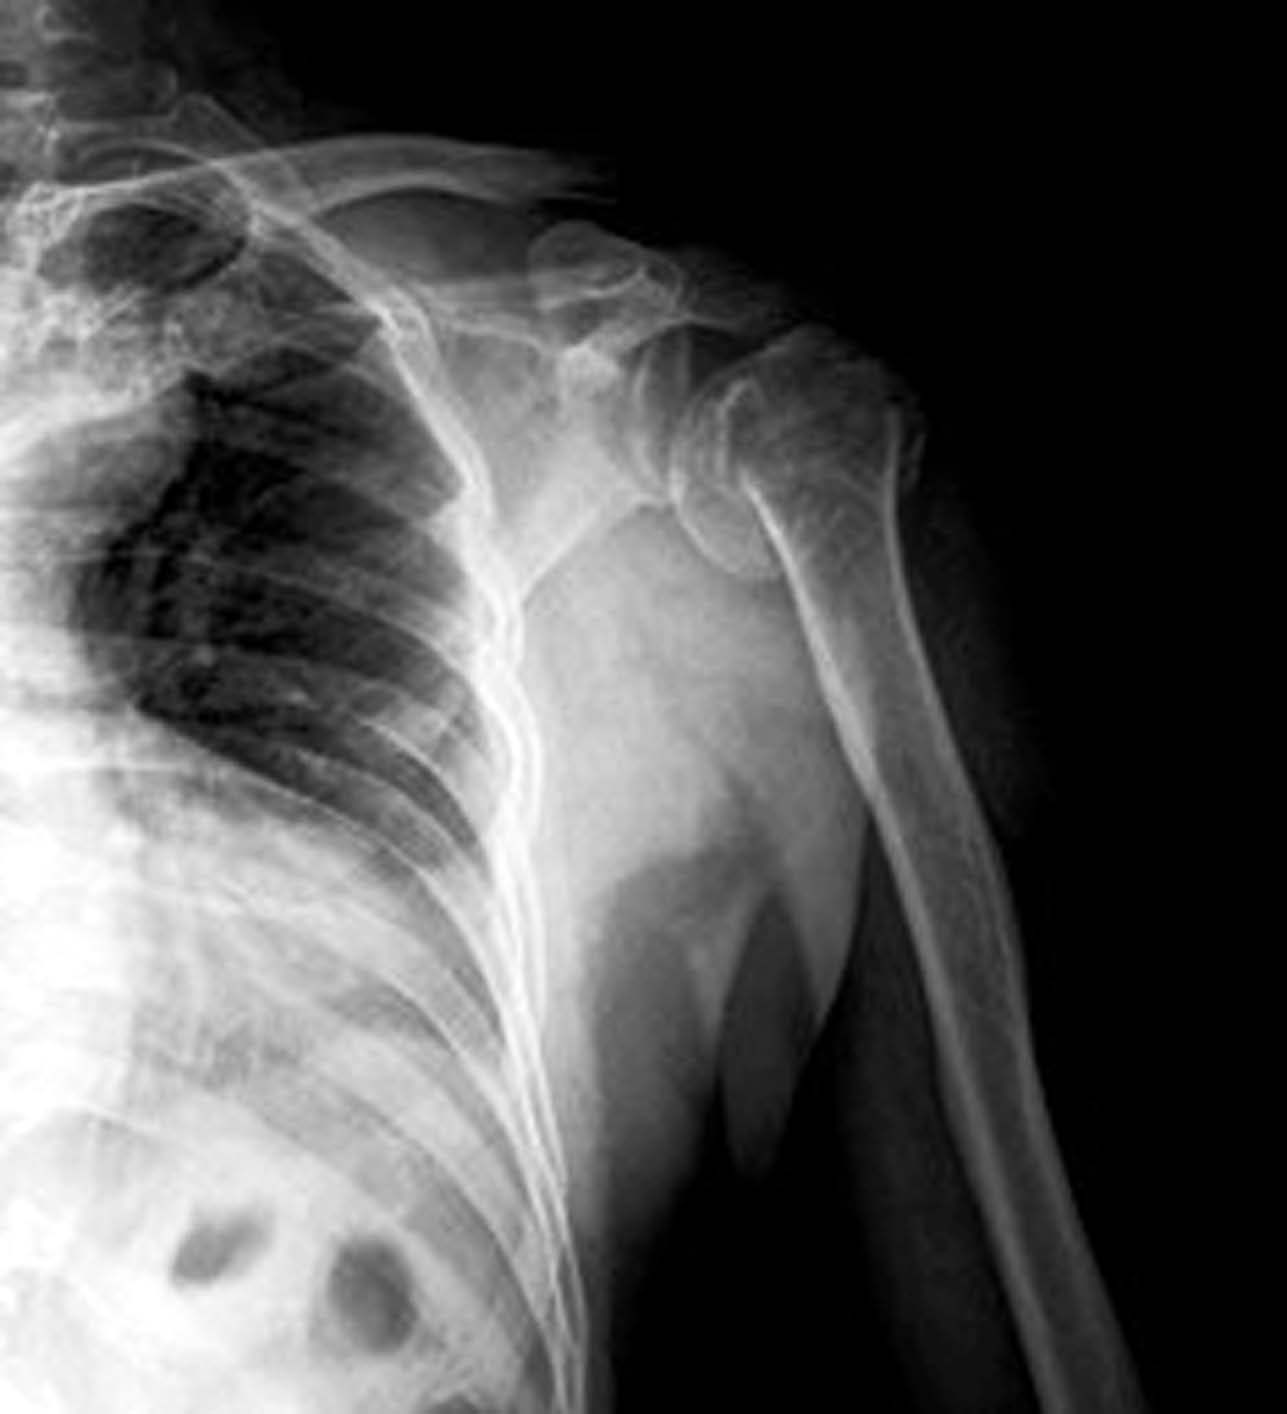
\includegraphics[width=.7\textwidth,height=\textheight,keepaspectratio]{./images/Image00030.jpg}
 \captionsetup{justification=centering}
 \caption{新生儿缺氧缺血性脑病\\{\small  A.左右额、顶叶白质区云絮状低密度灶,CT值约14~16Hu;B.皮层灰质薄,密度相对较高,灰白质分界欠清楚}}
 \label{fig2-14}}
  \end{figure} 



\textbf{【CT分度】}
①轻度:脑实质低密度影分布于1~2个脑叶,少数合并少量颅内出血(多为蛛网膜下腔出血)。②中度:低密度影超过2个脑叶,灰白质界限模糊,部分脑沟消失,约1/3合并颅内出血。③重度:弥漫性低密度影,灰白质界限消失。基底节、丘脑密度正常,脑室受压变窄,并发颅内出血者约占80%。

但我们认为对于超过2个脑叶者,如位于各叶的病灶面积均较小,且灰白质界限较清晰者,应诊断为轻度,以便于与临床分度相对应。

\textbf{【并发症】}
①轻度者于1~2个月病变多吸收,无明显后遗症。②中度者大多数亦可治愈,少数可出现外部性脑积水、脑发育不良、脑萎缩等。③重度者约35%于1周内死亡,存活者多有后遗症如脑萎缩、脑皮质变薄、脑白质减少、脑白质变性、脑软化、脑穿通畸形、钙化等。有报道病变处CT值<12Hu的重度患者多有并发症。

\textbf{【鉴别诊断】}
早产儿脑CT表现为较广泛的或弥漫性白质低密度区;皮层变薄、密度相对增高,呈花环状改变;灰白质分界清楚,脑室系统未见异常,中线结构无移位。早产儿缺氧性脑损伤灰白质界限模糊(图\ref{fig2-14}B),有颅内出血和脑室旁出血性脑梗死、脑室周围白质和脑白质发育不良及脑梗死等。两者CT表现有所区别,但早产儿合并缺氧性脑损伤时,CT难以分级。

\subsection{新生儿颅内出血}

本病是新生儿常见的急症,为新生儿死亡和以后神经发育障碍的主要原因之一。

\textbf{【病因病理】}
病因主要有新生儿缺氧缺血性脑病、产伤、早产,少数为出血性疾病、颅内先天性血管畸形。①缺氧使脑组织充血、水肿、脑血管壁通透性增高,引起渗血或点状出血;同时缺氧可使肝脏合成凝血因子发生障碍,从而加重出血。②产伤可造成硬膜窦撕裂或皮质桥静脉、脑内的静脉以及脉络丛静脉破裂。出血常见部位为硬膜下,其次为蛛网膜下腔,也可发生于脑实质、脑室内或硬膜外。③原发性出血性疾病、颅内先天性血管畸形引起的出血很少见,前者多位于蛛网膜下腔,后者可在蛛网膜下腔或脑实质内。

\textbf{【临床表现】}
少量出血时可无症状,量多时可出现激惹、尖叫、惊厥、烦躁不安、呕吐等症状,2天后出现抑制症状如嗜睡、拒奶、昏迷、四肢张力低下及呼吸不规则、青紫等。

\textbf{【CT表现】}

1.硬膜下出血:多见于足月儿,常有头皮血肿、颅骨骨折、颅缝分离。

2.蛛网膜下腔出血:最常见,有3个特征性征象。①空三角征:又称矢状窦旁征,血液积聚于矢状窦旁呈高密度,静脉窦内流动的血液呈相对低密度,底边为颅骨,形成空心形△征象。②高脚杯征:又称天幕缘征,即血液沉积于小脑幕缘上下形成“Y”或“V”形高密度影。③纵裂池边缘模糊征:即纵裂池内出血高密度影边缘模糊。以上3个征象的出现率可达50%~80%(图\ref{fig2-15})。此外,有学者认为“直窦”宽>5mm可认为有出血。

\begin{figure}[!htbp]
 {\centering
 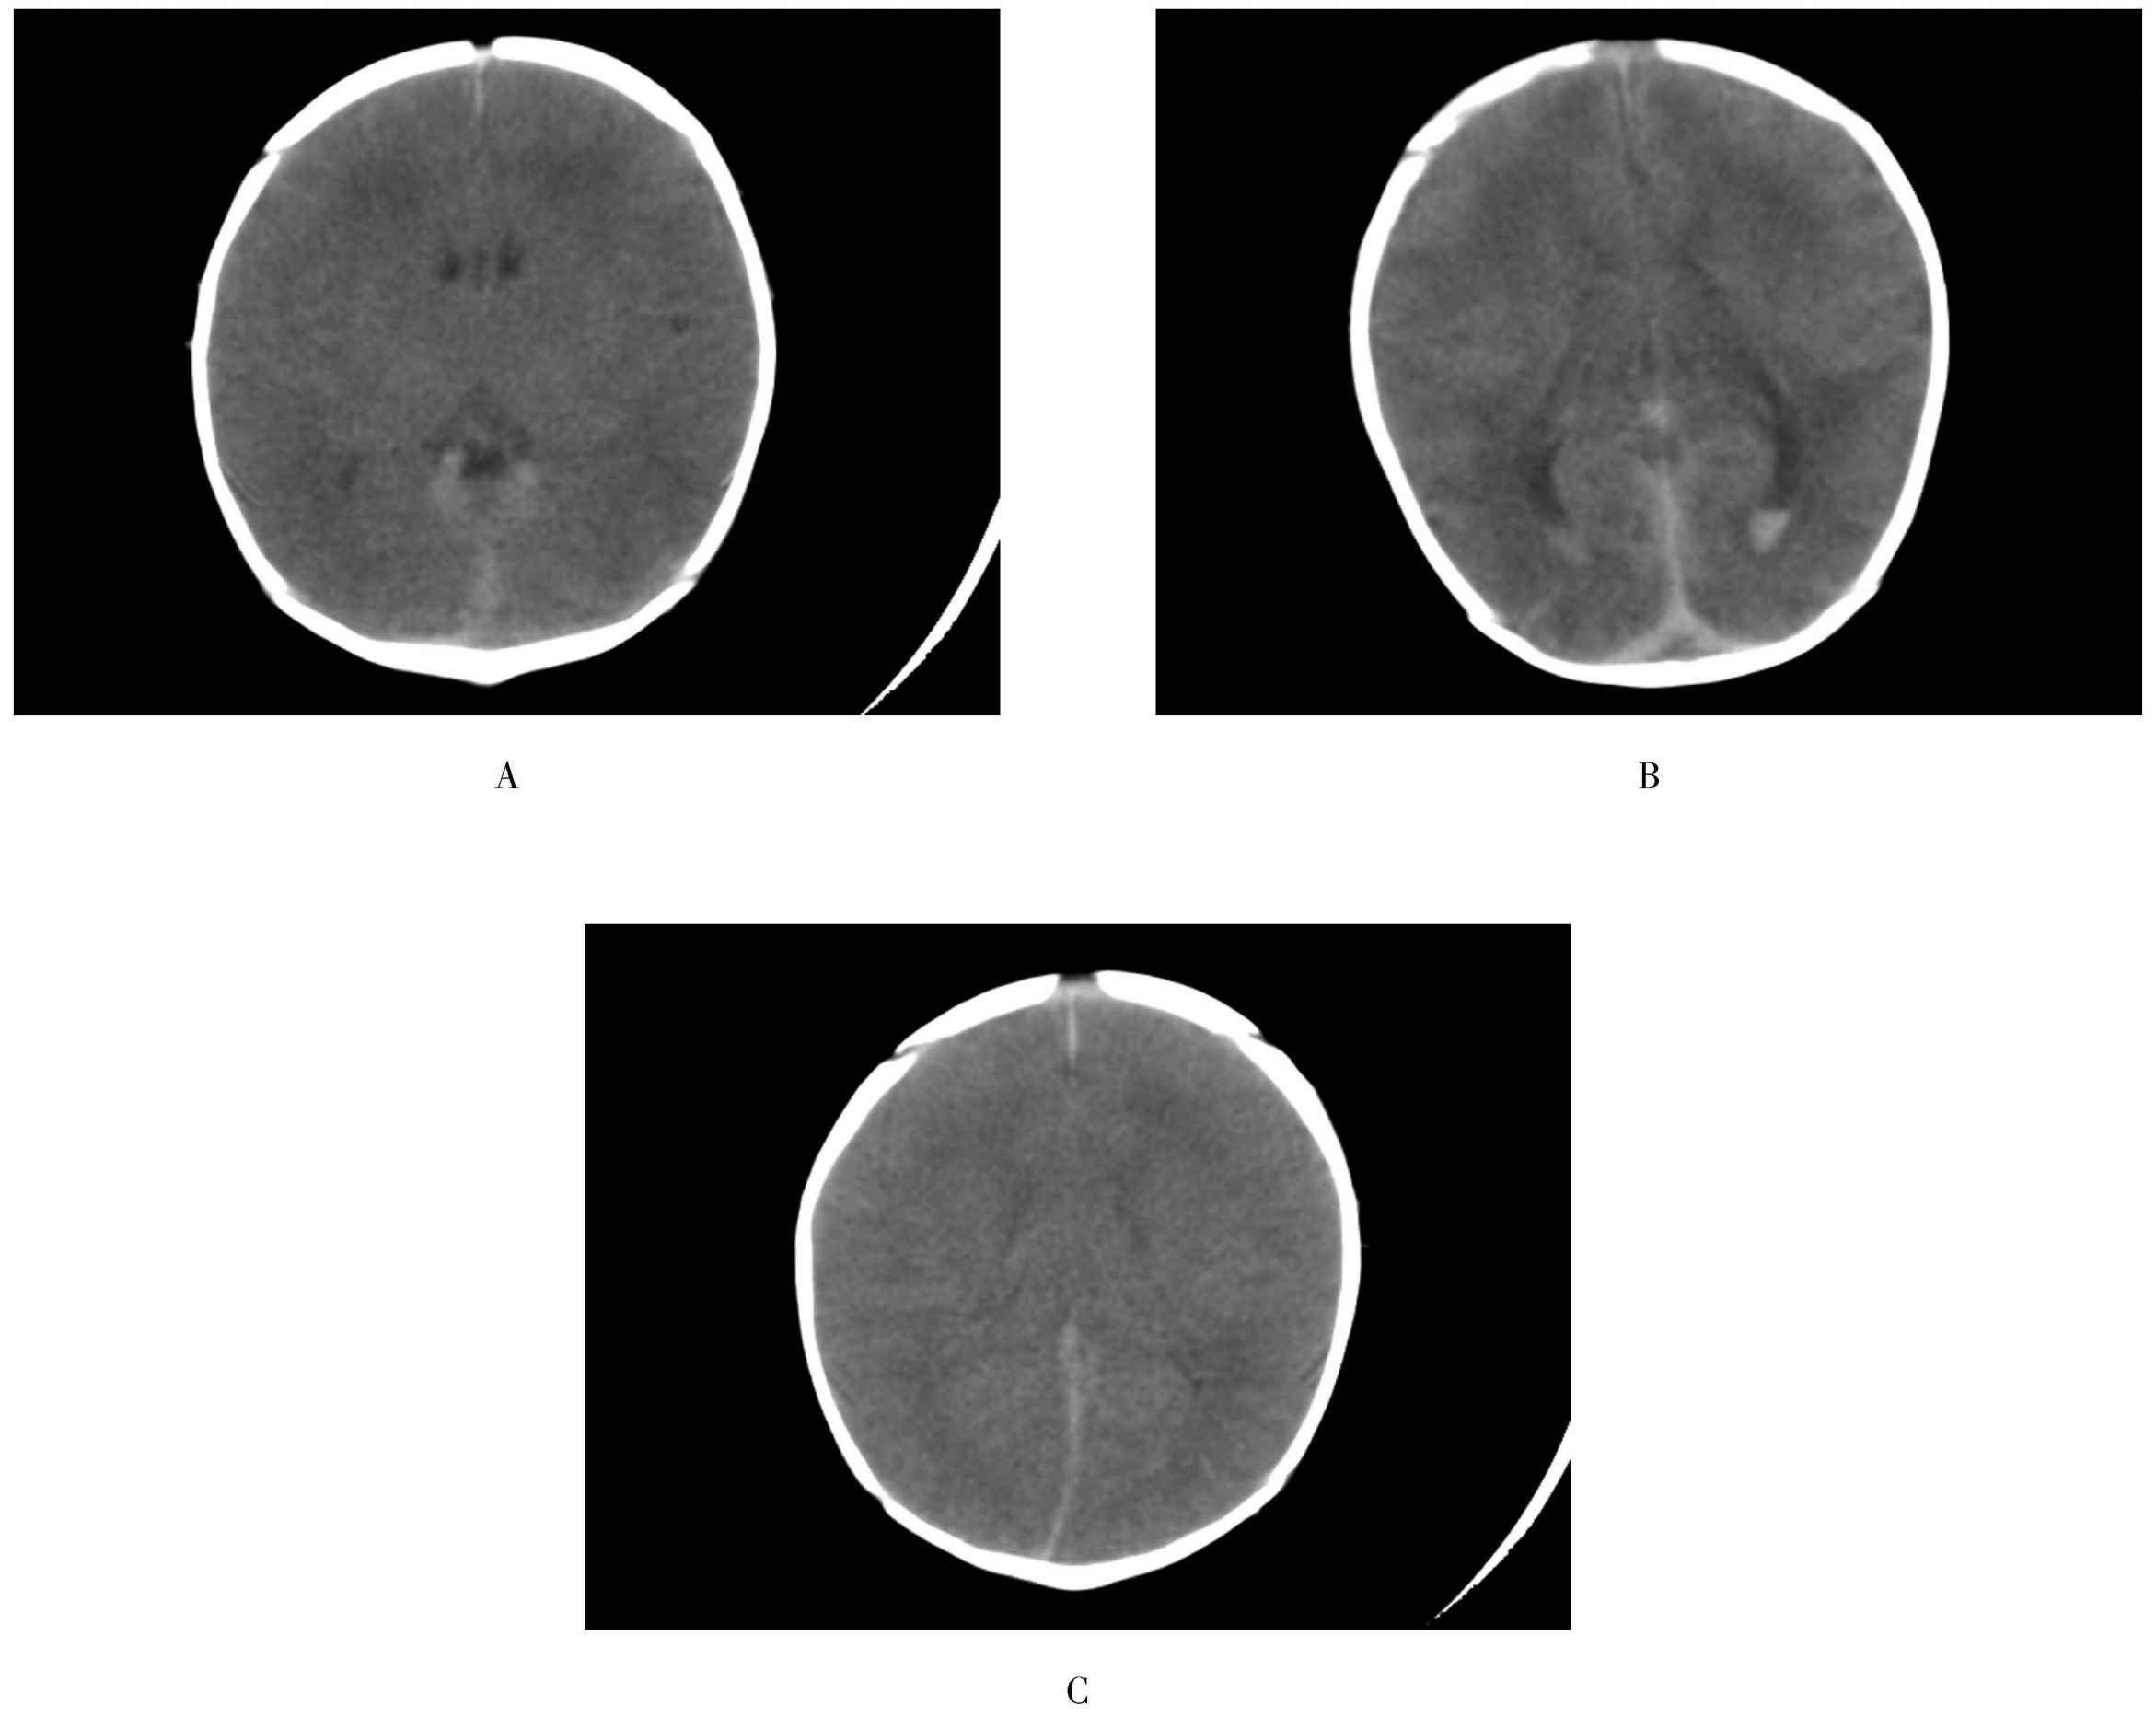
\includegraphics[width=.7\textwidth,height=\textheight,keepaspectratio]{./images/Image00031.jpg}
 \captionsetup{justification=centering}
 \caption{新生儿蛛网膜下腔出血\\{\small  A.高脚杯征;B.空三角征,伴有脑室内出血;C.纵裂池边缘模糊征}}
 \label{fig2-15}}
  \end{figure} 



3.脑实质内出血:呈点状或斑片状高密度灶,有或无水肿带。

4.室管膜下及脑室内出血:常见于早产儿。因室管膜下胚胎生发层组织发育不成熟,血液极易渗出,多量渗出可破入侧脑室,并可致脑积水。

5.其他:包括硬膜外出血和小脑出血,均较少见。

\textbf{【鉴别诊断】}
①钙化:新生儿颅内出血CT值为50~80Hu,新生儿颅内钙化少见且均为病理性,CT值>80Hu,因此不难鉴别。②晚发性维生素K缺乏症:发病年龄多在1~2个月小婴儿,出血量大、部位多,常有血团块形成、液平面出现及伴有脑梗死、大面积水肿,可予鉴别。

\subsection{婴儿维生素K缺乏症}

本病又称迟发性维生素K缺乏症、晚发性维生素K缺乏症,是指新生儿晚期(出生后2周)至乳儿期,因缺乏维生素K而引起的出血性疾病。

\textbf{【病因病理】}
常见的原因有3种:①维生素K摄入不足;②合成障碍;③吸收不良。维生素K是合成多种凝血因子所必需的辅酶,缺乏凝血因子凝血活性丧失,造成自发出血。

\textbf{【临床表现】}
发热、惊厥抽搐、呕吐、烦躁不安、拒乳、嗜睡等;可伴皮肤、消化道、上呼吸道出血等,并出现相应表现。婴儿期特别是1~4个月内母乳喂养儿若出现进行性贫血、全身出血倾向并伴急性颅内高压等精神症状应首先考虑本病。实验室凝血时间、凝血酶原时间延长及部分凝血活酶原时间延长可肯定诊断。

\textbf{【CT表现】}
①颅内出血:特点为出血量大,多发部位出血(脑实质内、外或脑室等);②脑水肿、脑梗死:是由于血管受挤压或痉挛所致,可呈广泛小片状水肿表现或大面积梗死,甚至半球缺血性改变;③脑疝;④一侧侧脑室闭塞,对侧侧脑室扩张积水;⑤并发症:存活者可致外部性脑积水、脑软化、脑萎缩、脑穿通畸形或脑发育不良。

\subsection{新生儿胆红素脑病}

持久性或明显的新生儿高胆红素血症可以导致脑部损伤。

\textbf{【病因病理】}
最常见的原因是红细胞溶血,其他原因包括红细胞增多症、胆红素结合方面的遗传或获得性缺陷、消化道运转方面的疾患及激素的紊乱等。未结合胆红素进入脑组织,结合于脑细胞膜,抑制细胞线粒体酶的活性,使脑细胞能量代谢障碍,致脑部损伤。

\textbf{【临床表现】}
足月儿常在生后2~5天,早产儿常在7天左右发生本病。典型的临床表现分为4期:①警告期;②痉挛期;③恢复期;④后遗症期。

\textbf{【CT表现】}
尚无报道本病有特异性CT表现。MR在急性期呈短T1和长T2信号;慢性期苍白球、下丘脑和海马显示长T2信号。

\subsection{血钠过高性脱水}

\textbf{【病因病理】}
最常见的原因是严重的腹泻,钠在细胞间隙中浓度升高致细胞内液体减少并皱缩。脑离开颅板导致桥静脉撕裂,另外血液的高渗致毛细血管增粗,易发生毛细血管破裂及脑实质出血。

\textbf{【临床表现】}
年幼儿童,尤其是未成熟儿对血钠过高有易感性。病儿极度冷漠、对刺激易激性高,另外还有肌肉强直、反射亢进,偶有癫痫。

\textbf{【CT表现】}
间质水肿引起脑实质密度降低,在大脑和小脑灰白质交界处可见高密度出血灶。

\subsection{新生儿低血糖症}

低血糖的标准是足月儿血糖低于16.7mmol/L(300mg/L),未成熟儿低于11mmol/L(200mg/L)。大多数低血糖的新生儿发病早,持续时间短,对葡萄糖反应迅速。但足月小样儿在子宫内就遭受营养不良,大多有临床症状,低血糖程度相对较重,持续时间可以延长,治疗需大量的葡萄糖。引起脑损害最通常的原因是继发于胰腺β细胞的先天性肿瘤或增生性胰岛素分泌过多。

\textbf{【CT表现】}
围产期低血糖脑损害表现为:①急性期:皮质和皮质下白质的脑水肿,以顶枕部最重;②慢性期:皮质和皮质下白质萎缩。

\subsection{外部性脑积水}

本病亦称良性蛛网膜下腔增宽,是一种特殊的交通性脑积水。一般2岁内自愈。

\textbf{【病因病理】}
有新生儿缺氧缺血性脑病、出血、外伤、感染等,半数病因不明为特发性。其发病机制可能为蛛网膜颗粒对脑脊液的吸收障碍所致。多数学者认为颅缝开放是其发生的前提。

\textbf{【临床表现】}
抽搐(约占50%以上)和头围增大(占1/3~2/3);部分患儿无症状。抽搐的发生与本病的严重程度密切相关。本病好发于2~24月前囟未闭的小儿,但可在生后数天发生,3~6个月为典型期,9个月~1岁开始好转,2岁前或囟门闭合前基本恢复正常。

\textbf{【CT表现】}
额叶或额、顶叶蛛网膜下腔间隙>5mm,而后部不宽。前纵裂池增宽>7mm,后纵裂池不宽。外侧裂池增宽>7mm。鞍上池稍大。额、顶叶脑沟部分增宽,但增深不著。大脑后半部及小脑正常。脑室正常或轻度扩大(图\ref{fig2-16})。

\begin{figure}[!htbp]
 {\centering
 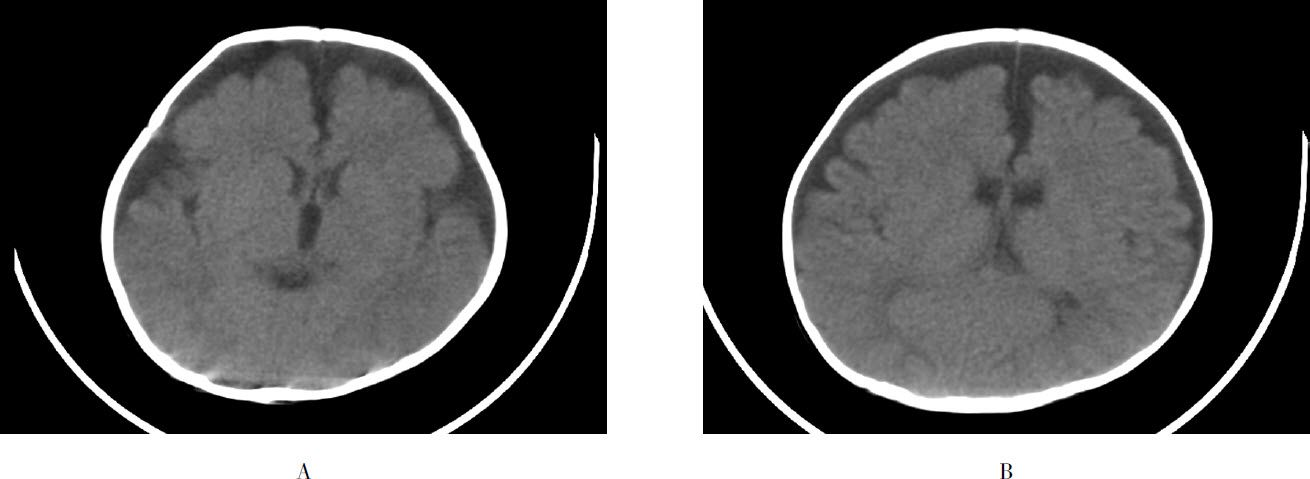
\includegraphics[width=.7\textwidth,height=\textheight,keepaspectratio]{./images/Image00032.jpg}
 \captionsetup{justification=centering}
 \caption{外部性脑积水\\{\small  A、B为同一患者,额、顶叶蛛网膜下腔间隙>5mm,而后部不宽;前纵裂池增宽>7mm,后纵裂池不宽;外侧裂池增宽>7mm}}
 \label{fig2-16}}
  \end{figure} 



总之,本病诊断的依据是:①前囟未闭的婴儿及头颅增大;②脑前部脑外积液增多,脑实质无改变;③2岁后脑外积液自然吸收。

\textbf{【鉴别诊断】}

1.在诊断外部性脑积水时,应除外其他因素引起的蛛网膜下腔增宽,其中包括促肾上腺皮质激素和皮质类固醇的治疗、脱水、营养不良以及癌肿化疗等。

2.脑萎缩:①外部性脑积水头围大,常有抽搐,无智力低下及运动障碍;而脑萎缩头围小,常有智力低下及运动障碍。②前者仅脑的前部蛛网膜下腔增宽;而脑萎缩常全脑蛛网膜下腔及脑沟增深、增宽。③前者纵裂池增宽限于前部;而后者则为整个增宽。④前者脑皮质厚度正常,脑沟可增宽但增深不著;而后者脑皮质变薄,密度减低及脑沟普遍加深。⑤脑室大小不能用于两者的鉴别,因为外部性脑积水可有轻度脑室增大。但脑萎缩时脑室与颅脑横径之比大于正常,而外部性脑积水正常。双额叶局限性脑萎缩时鉴别有一定难度,其双侧额角的局限扩大有助于与外部性脑积水鉴别。

3.硬膜下积液:本病多为单侧,双侧时常不对称,脑沟相互聚拢而不是加深加宽,不难鉴别。

4.脑发育迟缓:多表现为灰白质比例失常,常合并其他多种神经系统畸形。

\subsection{儿童脑室周围白质软化症}

本病又称为脑室周围萎缩、脑室周围白质发育不良,多认为好发于早产儿及产后窒息存活的儿童。

\textbf{【病因病理】}
与缺血缺氧及感染有关,主要损伤轴索及少突胶质细胞,但发病机制尚不清楚。病变主要分布于侧脑室三角区及枕角周围白质、额角附近白质。病理上脑白质由于缺血缺氧发生水肿、凝固、坏死,继而吸收或形成瘢痕和胶质增生,弥漫或局限的胶质损伤使髓鞘化延迟、白质减少,从而导致侧脑室扩张。

\textbf{【临床表现】}
本病可以导致脑瘫(主要是痉挛性下肢瘫或四肢瘫)、智力落后、抽搐,以及各种眼的异常如眼颤、斜视、视力下降等。

\textbf{【CT表现】}
显示脑室周围和半卵圆中心的脑白质明显减少,皮质与脑室缘距离甚小或消失,也可见呈斑片状或长条状的软化灶(图\ref{fig2-17})。一侧或两侧侧脑室扩大,扩大的脑室轮廓不规则可与脑积水鉴别。

\begin{figure}[!htbp]
 \centering
 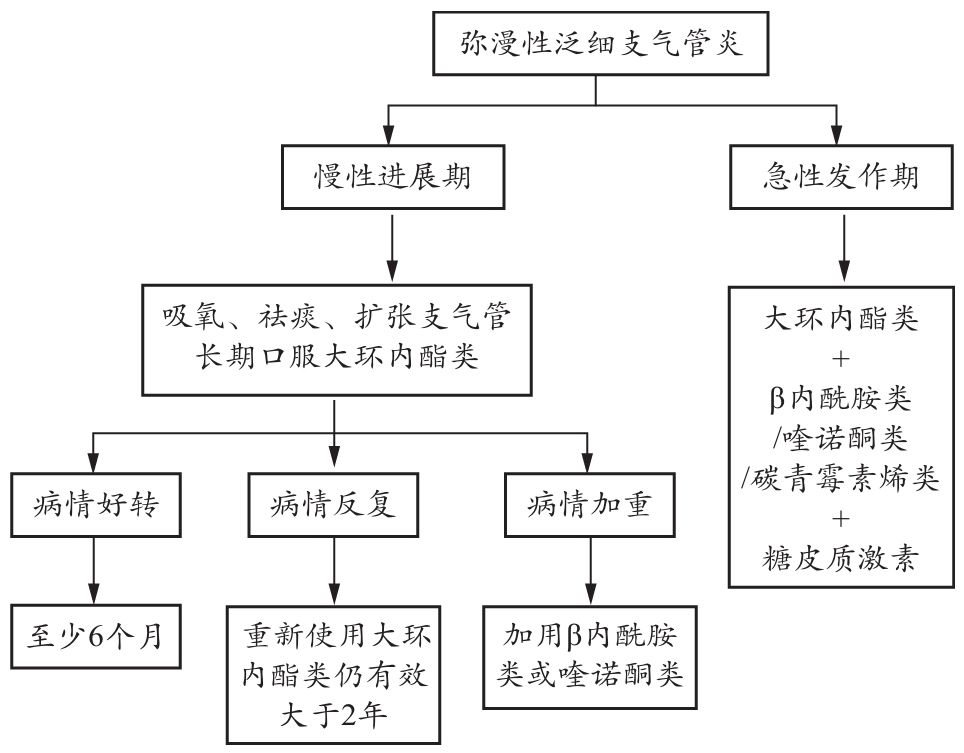
\includegraphics[width=.7\textwidth,height=\textheight,keepaspectratio]{./images/Image00033.jpg}
 \captionsetup{justification=centering}
 \caption{脑室周围白质软化症\\{\small 脑室周围和半卵圆中心的脑白质明显减少(右侧显著),皮质与脑室缘距离甚小,右侧有斑片状软化灶}}
 \label{fig2-17}
  \end{figure} 



\subsection{儿童脑性瘫痪的相关疾病}

本病是指出生前至出生后1个月内各种原因所致的非进行性脑损害综合征。临床表现为中枢性运动障碍及姿势异常,可伴智力低下、癫痫、视力障碍及行为异常。其CT改变可分为以下6种类型。

1.脑发育畸形:可分为器官源性和组织源性(已于上节详述)。

2.脑萎缩:大多由于缺血性损害或颅内感染导致脑白质或灰质减少、丧失,是脑性瘫痪最常见的CT表现。①可表现为脑沟裂增宽、增深,脑室增宽等。②其中脑室周围白质软化(PVL)约占脑萎缩的65%。③小脑萎缩可见小脑上沟增多(3条或3条以上)。

3.脑软化灶:多发生于较成熟的脑组织,可能与新生儿缺氧缺血性损害及颅内出血有关。

4.基底节病变:多由于脑血管阻塞致脑缺血缺氧性损害以及颅内感染、出血或中毒引起苍白球、丘脑区铁钙质沉着及神经细胞变性坏死。CT表现一侧或两侧对称性钙化灶或软化灶。

5.混合型:即上述两种以上病变混合存在。

6.正常:其原因可能为:①CT未能显示全部病灶或遗漏;②少数脑瘫与病变部位神经递质异常有关,CT不能显示;③胎儿期囊性病灶出生后自行消失;④CT检查的局限性,如CT难以显示矢状窦旁区脑损害及髓鞘形成延迟或发育不良。

\section{脑积水}

\subsection{概述}

1.脑积水:是指由于脑积液的产生和吸收不平衡所致的脑室扩大。按其发病机理可分为两大类:①脑脊液循环或吸收障碍;②脑脊液分泌增加。后者非常少见,主要见于脑室肿瘤如脉络丛乳头状瘤。脑脊液的吸收过去认为是通过蛛网膜颗粒,20世纪70年代后认为它不是惟一的吸收途径,并有学者认为主要是通过中枢神经系统表面吸收。

2.交通性脑积水:是指第四脑室出口以下的正常脑脊液通路受阻或吸收障碍所致的脑积水。国外有学者提出交通性脑积水应改称为动脉搏动限制性脑积水。动脉搏动明显减弱可能是由于动脉壁变硬或蛛网膜下腔顺应性降低所致。但动脉压并没有降低且传递的更远,使脑内脉压增高,大脑皮层压力梯度增大,脑室系统扩大。

3.阻塞性脑积水:又叫做非交通性脑积水,是指脑室系统即第四脑室出口以上任何部位发生阻塞所造成的脑积水,是最常见的脑积水。

脑积水时侧脑室旁白质内,CT上可见不规则低密度,是由于间质性水肿所致。即在脑室内压力增高时,室管膜受损出现小裂隙,水分子由此进入侧脑室周围白质内形成间质性水肿。高血压、动脉硬化及部分脑萎缩病人也可在室旁白质内出现上述CT表现(或异常MR信号),但其机理与脑积水不同,可能与局部组织变性、胶质增生、细胞萎缩后间隙扩大等有关。

\subsection{交通性脑积水}

\textbf{【病因】}
主要有蛛网膜下腔出血、脑膜炎、颅脑损伤以及静脉栓塞,亦可见于脑膜瘤病、脑脊液吸收功能障碍等。

\textbf{【临床表现】} 主要表现为颅内压增高的症状和体征。

\textbf{【CT表现】}
典型表现是脑室系统普遍扩大;另一特征是脑沟变浅、变平(但也可正常甚至扩张)。早期为颞角扩大和钝圆,稍后为额角扩大,进一步加重出现第三脑室扩大,第四脑室扩大较晚,与脑萎缩相比第三脑室扩大更明显。但有时交通性脑积水表现不典型,特别合并脑萎缩时,诊断较困难。此外,蛛网膜下腔出血和化脓性脑膜炎可表现为急性脑积水,脑室系统短时间内明显扩大。

交通性脑积水的特征之一为脑沟变浅、变平且灰白质界限清楚,常据此帮助诊断。但有时脑沟、脑池扩大,特别是纵裂池、基底池和桥小脑角池扩大。这种情况多见于基底池等有关脑池的炎症或肿瘤所致的部分脑脊液循环通路受阻及脑脊液吸收障碍。

脑室旁白质水肿发生率约为40%,且长期存在的交通性脑积水往往不出现这种征象。这是因为长期室内高压所致的室管膜受损,发生胶质增生形成室管膜瘢痕,阻止了脑脊液渗漏。

\subsection{正常压力性脑积水}

本病是交通性脑积水的一种特殊类型,多发生在慢性交通性脑积水的基础上,部分完好的脑脊液循环吸收功能代偿,且脑脊液的分泌功能下降,从而形成新的平衡。此时,虽然脑室系统仍明显扩大,但脑脊液压力正常,故又称为常压性脑积水。但实际上,大多并不一直正常,呈波动性。

\textbf{【临床表现】}
一般无颅内高压征,可能由于扩张侧脑室对周围白质的压迫,出现痴呆、步态不稳等症状。

\textbf{【CT表现】}
多不典型。由于脑室内压力正常,可在脑室扩大的同时出现脑沟加深,但两者不呈比例,脑室扩大更著。

\subsection{阻塞性脑积水}

\textbf{【病因病理】}
主要有先天性疾病、感染性疾病和肿瘤。病理表现为脑实质变薄,并可继发脑萎缩、白质脱髓鞘、胶质增生和神经细胞退行性变。

\textbf{【临床表现】}
主要为颅内压增高的症状和体征。其中先天异常、胎儿期或出生过程中发生该病者多在婴幼儿期出现症状,有的至10岁后或成年才表现异常。患儿有头颅增大,两眼球下旋形成“落日征”等甚有特点。

\textbf{【CT表现】}
阻塞近侧脑室扩大,阻塞远侧脑室形态正常或缩小(图\ref{fig2-18})。侧脑室旁间质水肿较明显而且范围广泛,脑沟也可变浅平,有时可见脑室疝。但病因诊断较困难。

\begin{figure}[!htbp]
 {\centering
 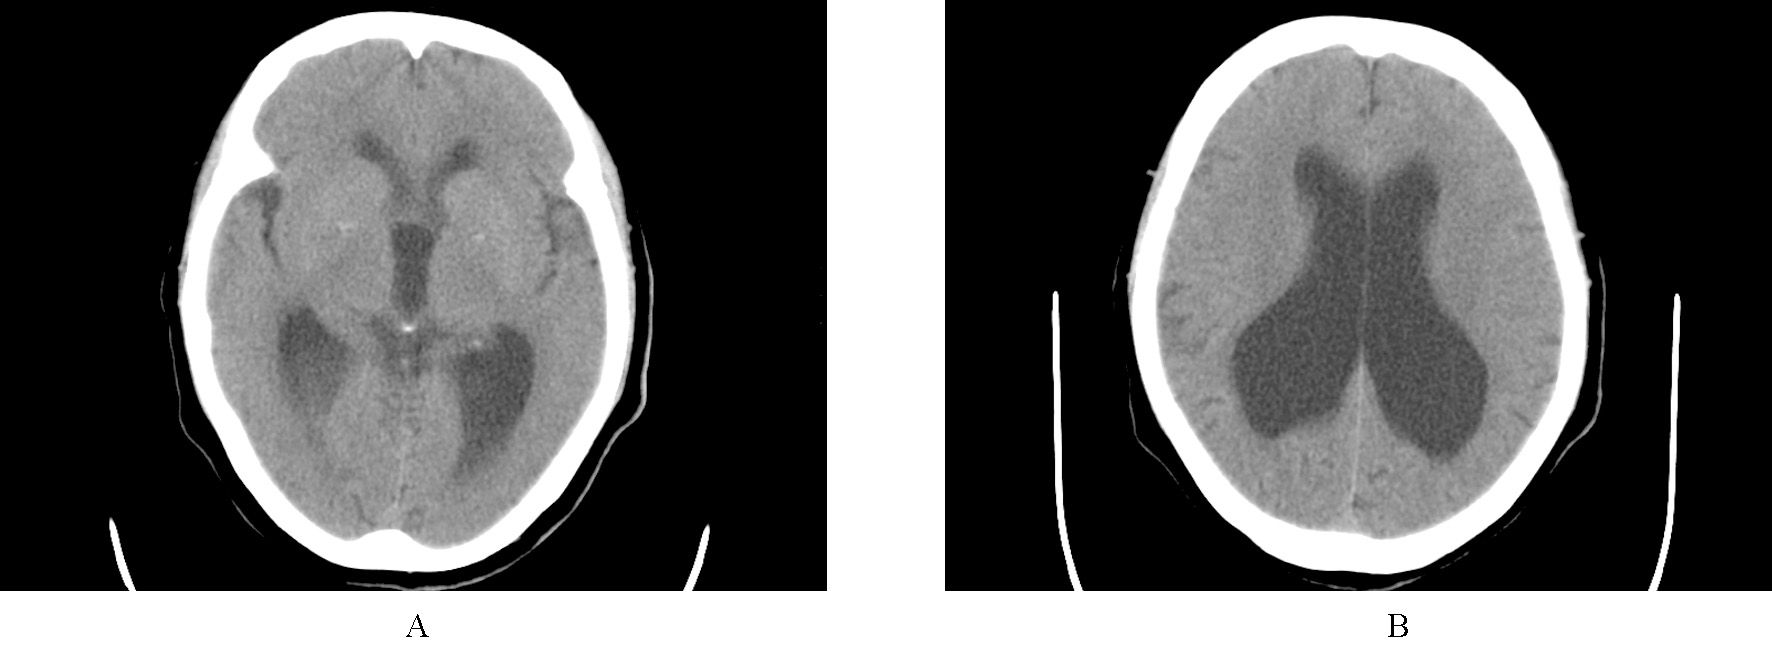
\includegraphics[width=.7\textwidth,height=\textheight,keepaspectratio]{./images/Image00034.jpg}
 \captionsetup{justification=centering}
 \caption{阻塞性脑积水\\{\small  A、B为同一患者,第三脑室、侧脑室扩大(第四脑室正常)}}
 \label{fig2-18}}
  \end{figure} 



先天性患者可重度积水,表现幕上大脑半球区为水样低密度,额、顶、颞叶脑实质几乎消失或残留极少,部分枕叶、基底核和丘脑保存(图\ref{fig2-10})。

\textbf{【鉴别诊断】}
与交通性脑积水鉴别时,如果阻塞在中脑导水管或以上,由于第四脑室不扩大,则两者容易鉴别。如阻塞部位在第四脑室出口时则两者难以鉴别。脑池造影观察第四脑室与蛛网膜下腔的通畅情况有助于鉴别。

\subsection{脑积水与脑萎缩的鉴别诊断}

主要有以下几点:①脑积水的扩大是均匀性和中心性扩张,尤其侧脑室前角呈气球状;而脑萎缩的脑室形态改变不及脑积水明显,特别是室旁脑组织较少的部位变形轻微,如第三脑室前壁、漏斗隐窝和视隐窝。②脑积水时由于颅内压力较高,脑沟变浅或消失,脑池亦不增大;而脑萎缩涉及皮质时脑沟加深、脑池扩大。③阻塞性脑积水和脑萎缩均可致一侧脑室扩大或一侧脑室扩大明显。在阻塞性脑积水时脑室可向扩大或扩大明显的对侧移位;而脑萎缩则向同侧移位。④脑积水侧脑室旁白质内可见间质性水肿所致的低密度;但脑萎缩因室旁白质变性亦可出现低密度灶。⑤脑萎缩是以白质为主的萎缩,表现为侧脑室边缘不规则,有助于与脑积水鉴别。

\section{脑萎缩}

\subsection{概述}

\subsubsection{脑变性疾病和脱髓鞘疾病的概念}

这是两组病变累及部位不同的神经系统疾病。前者累及神经元(灰质);后者累及髓鞘(白质),为髓鞘脱失,而轴索相对完好(见本章第十一节)。但两者均可引起脑萎缩。

变性疾病的特点是某一或二个功能系统的神经细胞发生萎缩和死亡,星形细胞增生。受累部位不同,临床表现也不同。如累及大脑皮质主要表现为痴呆;累及基底节、锥体外系则引起功能障碍;累及小脑引起共济失调。

脑变性疾病按部位分为:①大脑皮质:如Alzheimer病、Pick病。②基底节及脑干:如Jakob-Creutzfeldt综合征、Huntington舞蹈病、Parkinson病、进行性核上麻痹、Sky-Drager综合征。③脊髓及小脑:如橄榄桥脑小脑萎缩、原发性小脑萎缩、共济失调性毛细血管扩张症。④运动神经元:如脑萎缩性侧索硬化、脊髓性肌萎缩。

\subsubsection{脑萎缩的概念}

1.脑萎缩:是指由于各种原因所引起的脑组织减少而继发的脑室和蛛网膜下腔扩大。这种脑组织减少可分别或同时累及脑白质和脑灰质,其病因很多。根据其累及范围可分为局限性和弥漫性两类,但有时两者很难完全分开。

2.局限性脑萎缩:脑实质以局限性容积缩小为主,表现为局限性脑沟增宽和脑室、脑池扩大,有时仅发生于一侧半球。此外,还可见局部脑组织密度下降。

3.弥漫性脑萎缩:脑实质的减少为弥漫性,表现为脑室和蛛网膜下腔扩大广泛(图\ref{fig2-19})。可根据累及灰、白质程度的不同将其分为皮质型和中央型。前者以累及灰质为主,脑沟增宽明显,而脑室扩大次之;后者主要累及白质,以脑室扩大为主,脑沟扩大为次。

\begin{figure}[!htbp]
 \centering
 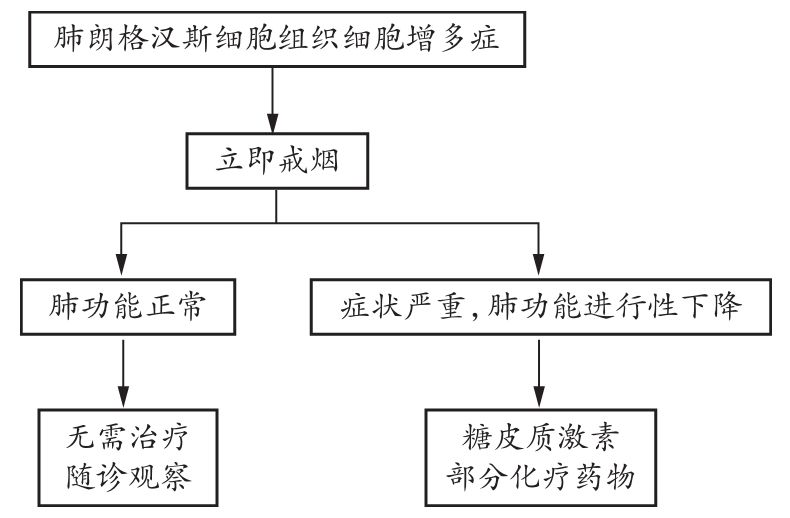
\includegraphics[width=.7\textwidth,height=\textheight,keepaspectratio]{./images/Image00035.jpg}
 \captionsetup{justification=centering}
 \caption{弥漫性脑萎缩\\{\small 脑室和蛛网膜下腔广泛扩大,室旁白质内有低密度灶,侧脑室边缘不规则}}
 \label{fig2-19}
  \end{figure} 



\subsubsection{局限性脑萎缩的病因}

1.外伤性脑萎缩:一般发生在外伤3~6个月后,少数外伤可造成弥漫性脑萎缩。

2.感染后脑萎缩:多继发于脑脓肿,颅内低毒性感染有时可造成弥漫性脑萎缩。

3.脑梗死后脑萎缩:一般发生在发病后3~6个月。

4.Pick病:又称脑叶萎缩症,系常染色体显性遗传性疾病。多见于女性,病程5~6年,呈进行性恶化。临床表现智力低下、痴呆、共济失调等,与Alzheimer病难以区别。但本病以额叶和颞叶萎缩为主,尤其以两额叶为著;而Alzheimer病为弥漫性脑萎缩,且以颞叶较著,额叶多不明显。

5.大脑半球萎缩:由于胎儿期或新生儿期血管阻塞引起的大块脑梗死所致,一般在青少年期才被发现。

\subsubsection{弥漫性脑萎缩的病因}

临床上较局限性脑萎缩更常见,多见于正常老年人,亦可见于许多病理情况。①Alzheimer病;②Huntington病;③Parkinson病;④Wilson病;⑤脑缺氧;⑥Jakob-Creutzfeldt综合征;⑦肿瘤和代谢失调:均与脑组织营养障碍有关(肿瘤患者虽无脑转移瘤,但可有营养障碍),同样情况也可见于AIDS、肝性脑病、血液透析者、慢性酒精中毒和肥胖病人;⑧药物性脑萎缩:如类固醇、氨基甲叶酸、度冷丁、酒精等使用不当。

\subsection{老年脑(生理性脑萎缩)}

关于老年脑的临床意义,目前认识尚不统一。这是因为正常情况下随着年龄的增加,脑组织和其他器官一样,逐渐老化而发生萎缩即所谓生理性萎缩。但随着年龄的增加,易发生的高血压、脑动脉硬化等因素均可损害脑组织而发生萎缩,这种萎缩虽与年龄有关,却为病理性。相对而言生理性萎缩较病理性萎缩轻,但两者无明显界限。

\textbf{【CT表现】}
老年脑主要表现为脑室、脑池轻度扩大和脑沟轻度增宽,多为两侧对称。脑沟增宽以额叶、镰旁顶叶显著,脑室扩大以侧脑室额角、颞角和第三脑室显著。

\subsection{Alzheimer病(爱茨海默病)}

本病以往曾称为早老性痴呆或老年前期痴呆,是一种以弥漫性脑萎缩(但以颞叶为主)为特征的痴呆。本病与老年性痴呆只有年龄上的差异而无本质的区别,故国际上将两病合并称为Alzheimer型痴呆。

\textbf{【病理】}
主要病理表现为脑萎缩,尤其是颞叶海马萎缩为主。镜下脑组织神经细胞减少,尤其有大量老年斑和神经纤维缠结时有定性价值,神经元空泡颗粒变性和淀粉样血管病变,但均为非特异性的,可见于老龄脑。

\textbf{【临床表现】}
其特征为进行性记忆力减退,语言和行为障碍。生前主要依据神经心理测验确立诊断。其病程不可逆转,一般持续3~10年,最后继发感染和全身衰竭而导致死亡。

\textbf{【CT表现】}
①弥漫性脑萎缩表现,与老年性脑萎缩相似,无特征性。②内侧颞叶萎缩是本病最早、最敏感的指征,以海马萎缩最突出,其次为额顶叶。主要表现为颞角扩大,颞叶皮质萎缩和海马回密度减低。有人取负于听眦线20\textsuperscript{o}
平面为扫描基线,层厚5mm,在环池水平测量颞角内侧边与环池外侧边的最小距离即中颞叶最小宽度,其参考值为8.67mm,小于此值即为中颞叶萎缩。③胼胝体萎缩为本病的另一指征,以嘴部和压部最为明显。④在海马萎缩的同时,MR、ECT(PET)等所显示的特异性区域血流量下降也可作为本病的特异性表现。

\textbf{【鉴别诊断】}
主要应于血管性痴呆鉴别。后者在我国老年人中占痴呆疾病的首位(西方占第二位),其颞角扩张不及Alzheimer病明显。严重的皮层下和脑室周围白质病变是多发性梗死型痴呆较典型的表现。

\subsection{慢性进行性舞蹈病}

本病又称遗传性舞蹈病、亨廷顿(Huntington)病,是基底节和大脑皮质变性的一种常染色体显性遗传性疾病。

\textbf{【病理】}
以尾状核及壳核萎缩明显,后期则额、顶叶皮质萎缩。镜下见神经元减少和胶质细胞增生。其生化改变为基底节中多巴胺含量过多,而γ-氨基丁酸及胆碱的含量减少。

\textbf{【临床表现】}
好发于20~50岁,其特征为慢性进行性舞蹈样动作和痴呆,多有遗传和家族史。

\textbf{【CT表现】}
主要为尾状核及壳核的萎缩。两侧尾状核头、体部相对缩小,可伴或不伴侧脑室(尤其额角)扩大和脑沟增宽,两侧壳核对称性低密度。一般只要出现尾状核萎缩即可以做出诊断,小脑和脑干也可萎缩。

\subsection{Parkinson病(帕金森病)}

本病又称震颤麻痹,可分为原发性和继发性两类。前者病因不明;后者可因脑动脉硬化、挫伤、基底节肿瘤、药物和化学物质中毒所致,又被称为Parkinson综合征。

\textbf{【病理】}
肉眼变化的特点是黑质和兰斑脱色。镜下可见该处的神经黑色素细胞丧失。黑质和苍白球神经元明显减少,局部萎缩及黑色素退变。中脑黑质致密带色素细胞大量丢失,桥脑兰斑色素细胞明显减少,脑有对称或非对称萎缩。黑质与兰斑均属儿茶酚胺能核团,分泌多巴胺;尾状核、壳核的神经元属胆碱能细胞,分泌乙酰胆碱。由于黑质神经元大量丧失,使多巴胺含量下降,从而使得对纹状体区乙酰胆碱的抑制作用下降,出现震颤麻痹。

\textbf{【临床表现】}
发生于中年以上,起病很缓慢,逐渐加剧。主要症状包括震颤、肌张力高(强直)、运动障碍、假面具样面容等。

\textbf{【CT表现】}
无特异性,主要为脑室扩大和弥漫性脑萎缩,有时合并基底节钙化,后者亦可见于正常人。CT所示的脑萎缩与临床所见的震颤麻痹的严重程度无明显关系。MR可有黑质(致密带)的萎缩及异常铁质沉积所致的低信号。

\subsection{肝豆状核变性}

本病又称Wilson(威尔逊)病,是一种常染色体隐性遗传的铜代谢障碍性疾病。

\textbf{【病理】}
由于肝脏合成血浆铜蓝蛋白的能力下降,引起肝脏、大脑基底节区和角膜的铜沉积,亦可累及额叶皮质、红核、黑质及齿状核及肾等处。脑受累部位变性、萎缩、胶质增生,甚至缺血坏死、软化。以豆状核软化、角膜色素环(K-F环)及小叶性肝硬化为三大主征。

\textbf{【临床表现】}
好发于10~25岁青少年,约1/3有家族史。基底节损害症状包括进行性加剧的震颤、僵直与多动症,皮质损害为衰退型精神障碍,有肝硬化和角膜色素环表现。

\textbf{【CT表现】}
少数可无异常发现。主要表现为豆状核低密度区,多为双侧,使豆状核界限不清。低密度区还可累及尾状核、齿状核、红核、额叶和丘脑等,部分还可见尾状核、大脑和小脑萎缩。

\textbf{【鉴别诊断】}

1.代谢性疾病:其中以肝豆状核变性最常见,还有亚急性坏死性脑脊髓病(Leigh病)、维生素B\textsubscript{1}
缺乏症,以及线粒体脑病、Kearns-Sayre综合征、海绵状脑白质营养不良、黏多糖病、Hallervorden-Spatz病、岩藻糖苷沉积症、先天性丙酮酸代谢障碍。

2.感染性疾病:EB病毒性脑炎、乙脑和腮腺炎病毒性脑炎等。

3.中毒性疾病:以一氧化碳中毒最常见,还有变质甘蔗中毒、大量硫化氢吸入中毒、甲醇中毒和氰化物中毒等。

此外,纹状体黑质变性(40~50岁发病,病程渐进,以帕金森综合征为首见症状,为锥体外系疾病或列入多系统变性)也可出现双侧壳核对称性低密度及全脑萎缩。国内有学者报道1例静脉窦血栓形成致双侧基底节对称性低密度。我们遇见1例尿毒症患者,表现为以内囊后肢为中心,部分涉及双侧豆状核的低密度。

\subsection{皮质纹状体脊髓变性}

本病又称Jakob-Creutzfeldt综合征、亚急性海绵状脑病、传染性病毒性痴呆。过去一直被纳入变性范围,现多认为是一种病毒感染性疾病。

\textbf{【病理】}
出现以灰质为主的明显脑萎缩。镜下皮质、大脑基底节、脊髓、小脑、丘脑、脑干及脊髓前角神经元变性。神经细胞脱失,脑实质空泡化伴胶质细胞增生,病灶区如海绵状,无炎性变化,白质多正常,晚期可受累。

\textbf{【临床表现】}
好发于40~70岁,主要表现为迅速发展的精神衰退和痴呆,并可出现锥体束、锥体外系及共济失调症状。80%死于发病后1年左右。

\textbf{【CT表现】}
大脑皮质弥漫性萎缩,脑沟、裂增宽增深,亦可见两侧脑室扩大。晚期脑白质受累可见低密度,无占位效应,无强化。本病进展快,短时间随访明显加重。

\subsection{小脑萎缩}

\textbf{【病因】}
本病可由变性性疾病、中毒、慢性酒精中毒、滥用药物等引起。发生于儿童的共济失调性毛细血管扩张症亦表现为以蚓部为主的小脑萎缩。此外橄榄桥脑小脑萎缩(或称橄榄桥脑小脑变性)也是共济失调的一个类型。

\textbf{【病理】}
病变主要在小脑、小脑脊髓束、锥体束、橄榄核,甚至累及大脑皮质,小脑萎缩皮质重于髓质。橄榄桥脑小脑萎缩除小脑萎缩外,还有桥脑、橄榄的明显萎缩,大脑皮质也可受累。

\textbf{【临床表现】}
成年发病,病程缓慢,可为10~40年。表现为小脑性共济失调,锥体束征、锥体外系征、视神经萎缩。

\textbf{【CT表现】}
应包括以下两个或两个以上征象(图\ref{fig2-20}):①小脑沟增宽>1mm(也有人认为\textgreater{}2mm);②小脑沟在半球超过2条,蚓部超过4条;③桥小脑角池扩大>1.5mm(应测量小脑上边缘与岩骨边缘间的距离);④第四脑室扩大;⑤小脑上池扩大。

\subsection{精神分裂症}

本病多有脑结构的异常。

\begin{figure}[!htbp]
 \centering
 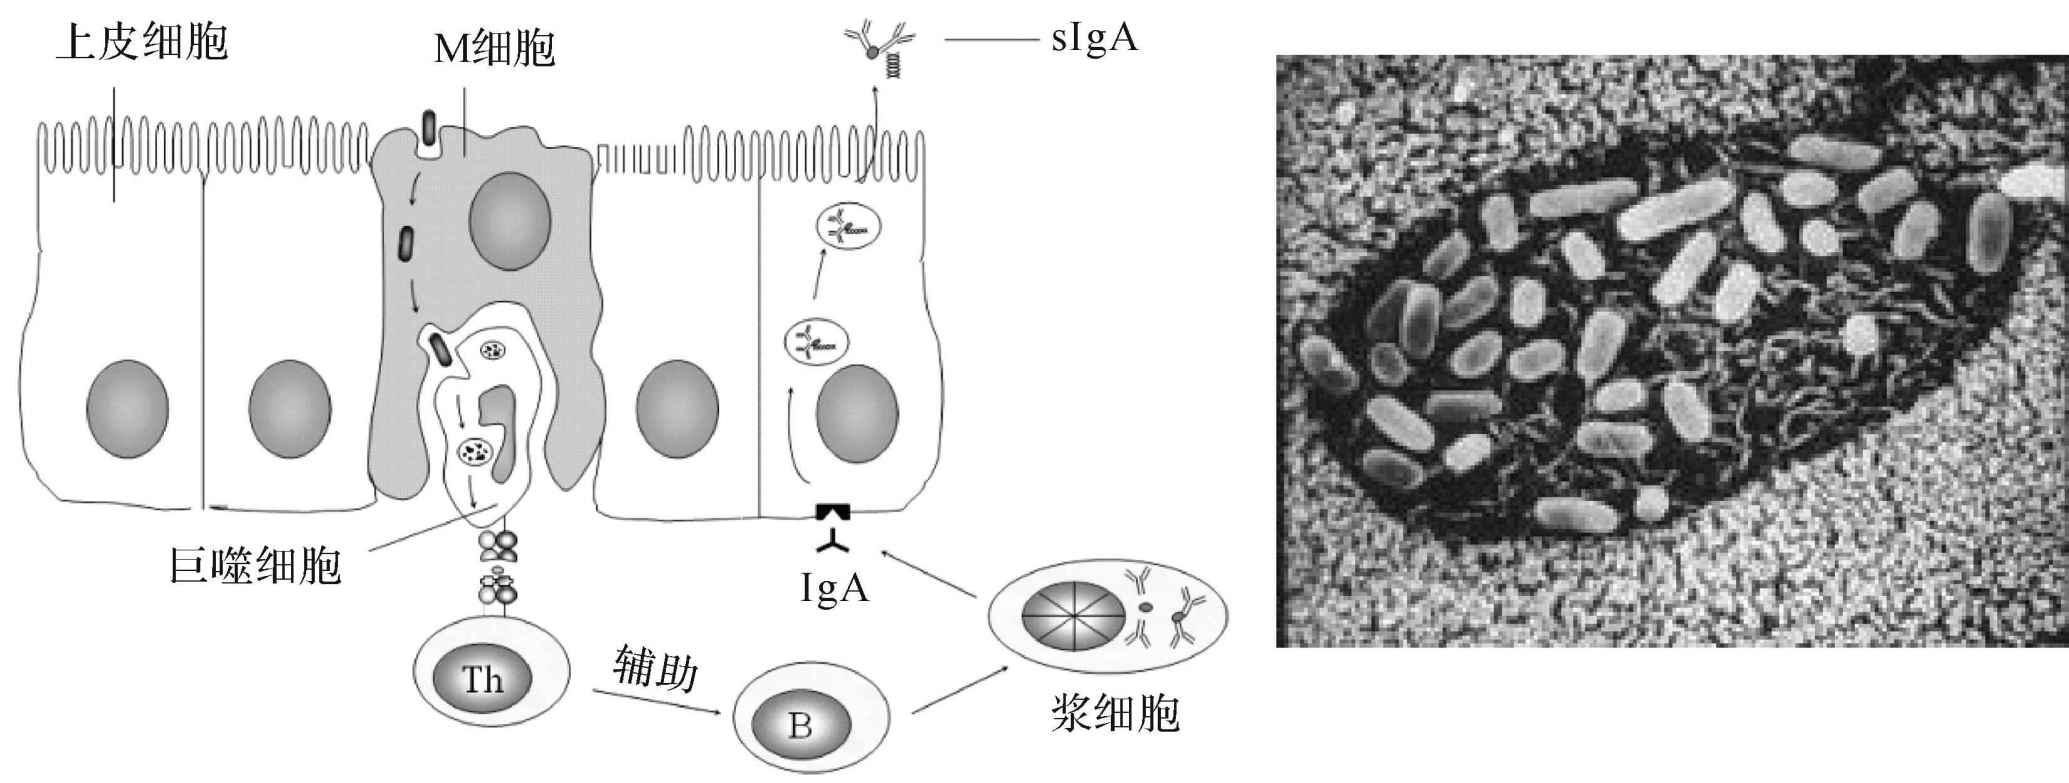
\includegraphics[width=.7\textwidth,height=\textheight,keepaspectratio]{./images/Image00036.jpg}
 \captionsetup{justification=centering}
 \caption{小脑萎缩\\{\small 小脑沟显著增宽、增多,以蚓部为著}}
 \label{fig2-20}
  \end{figure} 



\textbf{【CT表现】}
第三、第四脑室扩大,两侧裂池增宽、脑沟扩大,有时出现侧脑室扩大和小脑萎缩。两侧室旁核和小脑的密度可增加,其意义尚不肯定。

\subsection{颞叶癫痫}

颞叶癫痫的常见原因为海马硬化(又称安蒙氏角硬化和颞叶中内侧硬化)。

\textbf{【病理】} 特征为神经元丢失和胶质细胞增生,导致海马的萎缩。

\textbf{【CT表现】}
其CT诊断价值较小,仅约23.8%有异常。表现为:①颞叶内侧低密度灶;②颞角扩大;③侧裂池增宽。

\textbf{【MR表现】} 海马的萎缩(为神经元丢失的反应)、T\textsubscript{2}
WI海马高信号(为胶质细胞增生的反应)、颞叶前部萎缩以及颞角扩大。

\section{脑缺血、出血和脑血管病变}

\subsection{动脉缺血性脑梗死}

脑组织因血管阻塞引起缺血性坏死或软化称为脑梗死。广义的脑梗死除动脉缺血性脑梗死外,还包括静脉血流受阻所致的脑梗死即静脉性脑梗死。但大多习惯于狭义的将动脉缺血性脑梗死称为脑梗死。

\textbf{【病因】}
引起梗死的原因很多,可分为两大类。①脑血管阻塞:又分为血栓形成和栓塞。前者最常见的是在动脉粥样硬化的基础上形成血栓;后者是指外来栓子堵塞血管所致。②脑部血液循环障碍:是指在脑血管原有病变的基础上(亦可无原发血管病变),由各种原因造成的脑组织供血不全而引起的梗死,故又称非梗阻性脑梗死。

\textbf{【病理】}
过去将脑梗死分为3个时期,即梗死期、吞噬期、机化期。目前通常将脑梗死分为:①超急性期:6小时以内;②急性期:6小时后~2天;③亚急性期:2天后~2周内;④慢性早期:2周~1个月;⑤慢性晚期:1月后(见表\ref{tab2-2})。

\begin{table}[htbp]
\centering
\caption{脑梗死的病理过程及CT表现}
\label{tab2-2}
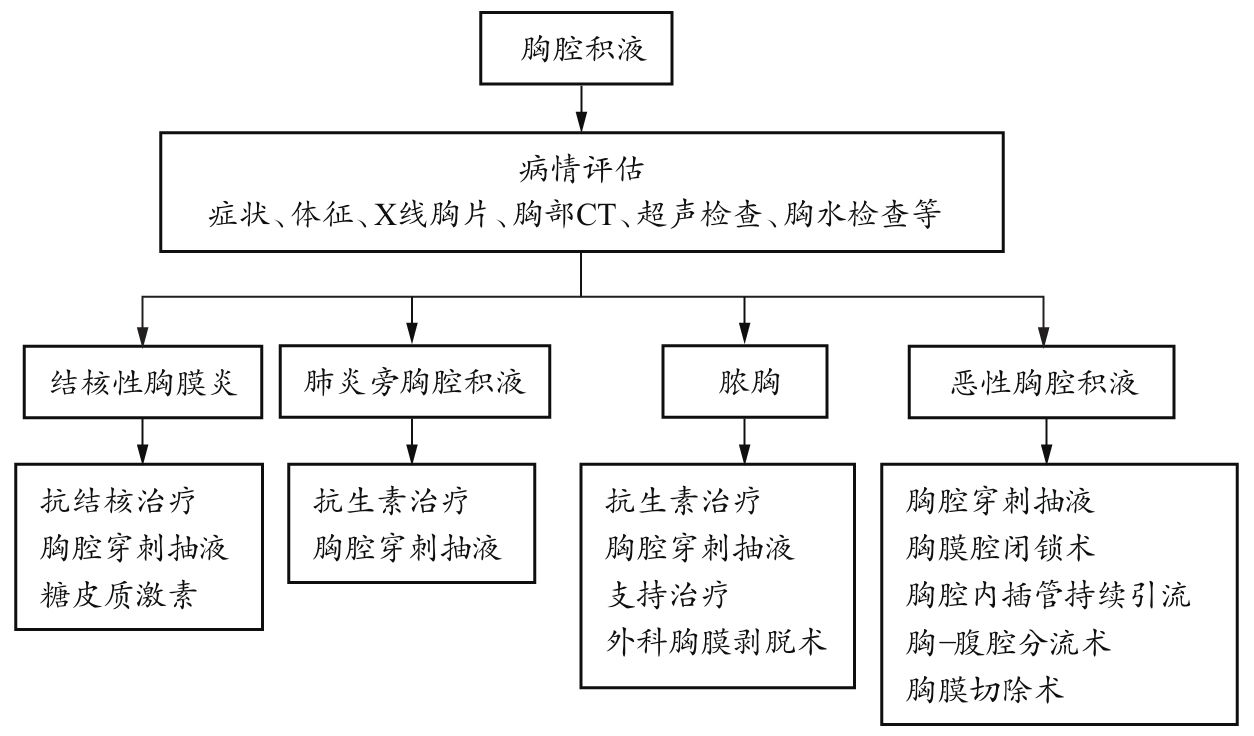
\includegraphics[width=\textwidth,height=\textheight,keepaspectratio]{./images/Image00037.jpg}
\end{table}

脑供血完全终止后数秒钟神经元电生理活动停止,持续5~10分钟以上就有不可恢复的细胞损伤。但是临床上供血血管闭塞可能不完全和(或)存在侧支循环,仅使局部血流降低到一定程度。故部分脑组织虽有缺血损伤,但仍可恢复正常,这部分脑组织区域称为缺血半暗带。它位于缺血坏死核心与正常脑组织之间。但如超急性期治疗不及时或治疗无效可发展成为完全脑梗死。

少数缺血性脑梗死在发病24~48小时后可因再灌注而发生梗死区内出血,称为出血性脑梗死。

\textbf{【临床表现】}
临床表现复杂,取决于梗死灶大小、部位及脑组织的病理生理反应。主要表现为头昏、头痛,部分有呕吐及精神症状,可有不同程度的昏迷。绝大多数出现不同程度的脑部损害症状,如偏瘫、偏身感觉障碍、偏盲,亦可失语、抽搐,较重者可有脑疝症状。从解剖学可知,皮质脊髓束有10%的纤维不交叉下降,加入同侧皮质脊髓侧束。皮质脊髓前束也有少量纤维不交叉,止于同侧颈、胸髓。这些不交叉的运动传导纤维支配了同侧肢体运动,当这些纤维受损时,导致同侧肢体出现不同程度的运动功能障碍如麻木、无力,甚至偏瘫。

\textbf{【CT表现】}

1.超急性期脑梗死的CT表现:①大脑中动脉高密度征:为高密度血栓或栓子所致,出现率约占35%~45%(敏感度78%,特异度93%),但需除外血管硬化因素。最近研究表明,此征可见于近60%的正常人(尤其用7mm以下层厚扫描),故此征的诊断价值值得怀疑。②脑实质低密度征:可能为细胞内水肿所致,可见于脑的凸面、基底节区、岛叶,有时可伴侧裂池受压。③局部脑组织肿胀征:可能为血管源性水肿所致,局部脑沟变窄以至消失,脑回增厚、变平(图\ref{fig2-21}A)。脑CT灌注成像有利于超急性期脑梗死的诊断。

此外,脑血管CTA可显示闭塞部位、程度和侧支循环情况。

许多学者研究证实,CT灌注成像可以预测半暗带,即脑血流量(rCBF)中度减低时,局部脑血容量(rCBV)无明显变化或仅有轻度下降或轻度升高,此时缺血区微血管管腔受压、变形、闭塞的程度较轻。当rCBF和rCBV均明显减低时,提示脑局部微血管管腔闭塞程度明显、微循环发生障碍、脑组织发生梗死。国内有学者将面积\textsubscript{CBV}
定义为预测的梗死面积,则面积\textsubscript{CBF} -
面积\textsubscript{CBV} 为预测的半暗带面积。

2.典型CT表现:①脑组织低密度灶,呈楔形或三角形,病灶部位、范围与闭塞动脉供血区相吻合。大脑中动脉主干闭塞,病灶呈三角形低密度区,尖端指向第三脑室;大脑中动脉闭塞在豆纹动脉的远端,病灶多为矩形低密度区,出现“基底核回避现象”。大脑前动脉闭塞表现为位于大脑镰旁的长条状低密度区。大脑后动脉闭塞在顶叶后部及枕叶可见半圆形的低密度区,位于大脑镰旁的后部。局灶性脑皮质梗死,表现为脑回丢失。室管膜下脑梗死,脑室边缘呈波浪状。一般在发病24小时后出现以上表现(图\ref{fig2-21}B、C)。②2~3周时由于“模糊效应”,病灶可偏小或消失。③脑梗死后2~15天为水肿高峰期,可有占位效应,占位效应一般见于病变范围大的病例。如占位效应超过1个月,应注意有无肿瘤可能。④增强扫描病灶周围和病灶内出现脑回状、线状、团块状强化。⑤1个月后病灶开始软化呈水样密度,病变范围大的病例可继发局限性脑萎缩。

此外,出血性脑梗死在梗死区内可见高密度出血灶(图\ref{fig2-21}D)。



\begin{figure}[!htbp]
 \centering
 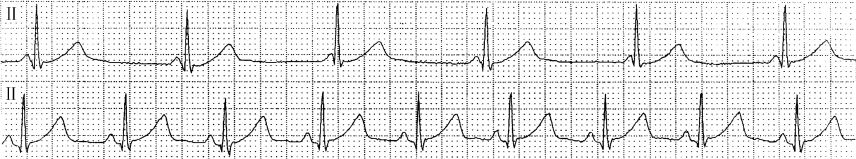
\includegraphics[width=\textwidth,height=\textheight,keepaspectratio]{./images/Image00038.jpg}
 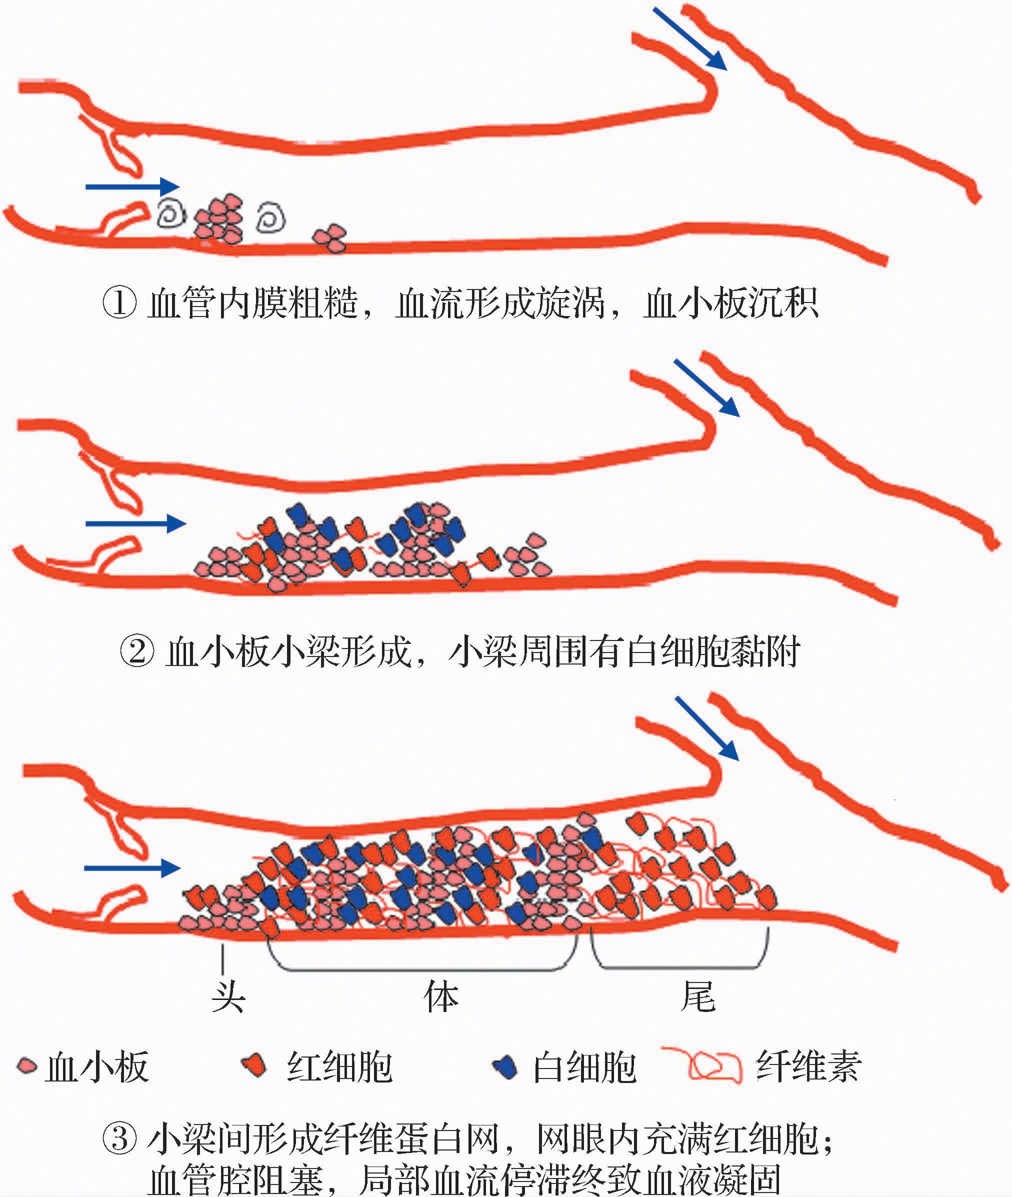
\includegraphics[width=\textwidth,height=\textheight,keepaspectratio]{./images/Image00039.jpg}
 \captionsetup{justification=centering}
 \caption{脑梗死\\{\small A、B为同一患者。A.超急性期,发病后4小时,右侧额顶叶脑沟消失,皮髓质交界不清晰;B.发病后42小时,右侧颞额顶叶大片状低密度灶,界限清晰,显著占位效应;C.亚急性期脑梗死,左侧顶额叶区有大片楔形低密度区,占位效应较显著;D.出血性脑梗死,右侧颞额叶区有大片楔形低密度区,占位效应显著,其内见大片状高密度出血灶,左侧基底节区可见水样密度的软化灶}}
 \label{fig2-21}
  \end{figure} 

3.增强扫描CT表现:梗死灶强化的形态多种多样,可表现为脑回状、线状、片状、环状,可出现在病灶的边缘和中心。而延迟30分钟~3小时扫描可显示皮质下白质强化,可能与梗塞区皮质内大量毛细血管破坏,造影剂漏出有关。其强化机制与缺血区血脑屏障受损,新生的毛细血管大量增生,以及局部血流量增加有关。但在1周内,虽有血脑屏障的破坏,却因局部缺血坏死严重,造影剂浓度亦相应很低,故一般不出现强化。梗死7~10天后因局部大量毛细血管增生,血流量增大而出现明显强化。2~3周发生率最高,强化最明显,可持续1个月或更久。

\textbf{【鉴别诊断】}
应注意与胶质瘤、转移瘤、脱髓鞘病变和脑脓肿等鉴别。①脑梗死常累及皮质和白质两部分;而上述病变一般只造成白质低密度。②脑梗死的分布为某一动脉区或分水岭区,有一定特征;而脑肿瘤和炎症水肿沿白质通道扩散,无明显分布规律,常呈指状低密度区;脱髓鞘低密度灶常对称性分布在侧脑室周围。③增强扫描胶质瘤常出现不均匀强化,有时可见壁结节;转移瘤常可见多灶强化。

\subsection{脑梗死前期}

从脑血流量(CBF)变化过程看,脑血流量的下降到急性脑梗死的发生经历了3个时期。首先,由于脑灌注压下降引起的脑局部的血流动力学异常改变;其次,脑循环储备力失代偿性低灌注所造成的神经元功能改变;最后,由于CBF下降超过了脑代谢储备力才发生不可逆转的神经元形态学改变即脑梗死。国内高培毅将前两者称为脑梗死前期,它不同于超急性期脑梗死。

他们根据脑局部微循环的变化程度以及CT灌注成像表现包括局部脑血流量(rCBF)、局部脑血容量(rCBV)、平均通过时间(MTT)和峰值时间(TTP)参数图,将脑梗死前期分为2期4个亚型:

Ⅰ期:脑血流动力学发生异常变化,脑血流灌注压在一定范围内波动时,机体可以通过小动脉和毛细血管平滑肌的代偿性扩张或收缩来维持脑血流相对动态稳定。

Ⅰ\textsubscript{1}
:脑血流速度发生变化,脑局部微血管尚无代偿性扩张。灌注成像见TTP延长,MTT、rCBF、rCBV正常。

Ⅰ\textsubscript{2} :脑局部微血管代偿性扩张。灌注成像见TTP
和MTT延长,rCBF正常或轻度下降,rCBV正常或轻度升高。

Ⅱ期:脑循环储备力失代偿,CBF达电衰竭阈值以下,神经元的功能出现异常,机体通过脑代谢储备力来维持神经元代谢的稳定。

Ⅱ\textsubscript{1}
:CBF下降,由于造成局部星形细胞足板肿胀,并开始压迫局部微血管。灌注成像见TTP
和MTT延长,以及rCBF下降,rCBV基本正常或轻度下降。

Ⅱ\textsubscript{2}
:星形细胞足板明显肿胀,并造成局部微血管受压变窄或闭塞,局部微循环障碍。灌注成像见TTP
和MTT延长,rCBF和rCBV下降。

\subsection{分水岭性脑梗死}

即指两条主要脑动脉供血交界区发生的脑梗死。

\textbf{【病因】}
①血液动力学障碍:低血压(如心肌梗死、心律失常、体位性低血压)等所致的血液动力学障碍;②血管调节功能失常:如糖尿病并发植物神经功能紊乱、长期低血压;③高血压病过分降压治疗;④心脏附壁血栓脱落沿血管进入脑皮质支和深穿支。

\textbf{【CT表现】}
①皮质下型:多为白质内低密度,常呈条形或类圆形。灰质由于血流再灌注而呈等密度,但灰质可出现明显强化。②皮质前型:额顶叶交界区三角形、条形低密度灶。③皮质后型:颞顶枕叶交界区三角形、条形低密度灶。

\subsection{血液动力性脑梗死}

当脑外动脉狭窄、部分阻塞和痉挛时,一般情况下尚能维持脑组织的血供。但当某些原因引起较长时间的血压下降时,可造成狭窄动脉供血脑组织的严重缺血而发生脑梗死,这种梗死称为血液动力性脑梗死。

\textbf{【病因病理】}
心律失常、心功能不全、休克、高血压过分降压等是其常见原因。严重的低血压和心搏量降低如心肌梗死、外科手术等,即使患者无颅内外血管病变,也可引起大脑半球的广泛梗死。血液动力性脑梗死多为分水岭性脑梗死。

\textbf{【CT表现】}
与分水岭性梗死的表现相似,可见条形或类圆形低密度,也可广泛梗死,这种梗死以分水岭区最著。可累及基底节区和小脑,皮质可强化。

\subsection{腔隙性脑梗死}

即指脑深部2~15mm大小的脑梗死。

\textbf{【病因】}
多为高血压、糖尿病、动脉硬化、高脂血症所致。好发于基底节、丘脑、内囊区、深部室旁白质及脑干。这些部位的血管多远离大脑主干,细长且走行弯曲,对血液动力学变化敏感,易受缺血影响。

\textbf{【临床表现】}
纯运动性偏瘫、纯感觉障碍、下肢运动受限、构音困难、视力障碍、失语、短小步态及共济失调等。

\textbf{【CT表现】}
梗死灶在2~15mm之间,呈圆形或卵圆形低密度,边缘不清,无水肿和占位效应。3~4周后可形成边缘清楚的囊性软化灶(图\ref{fig2-22})。

\begin{figure}[!htbp]
 \centering
 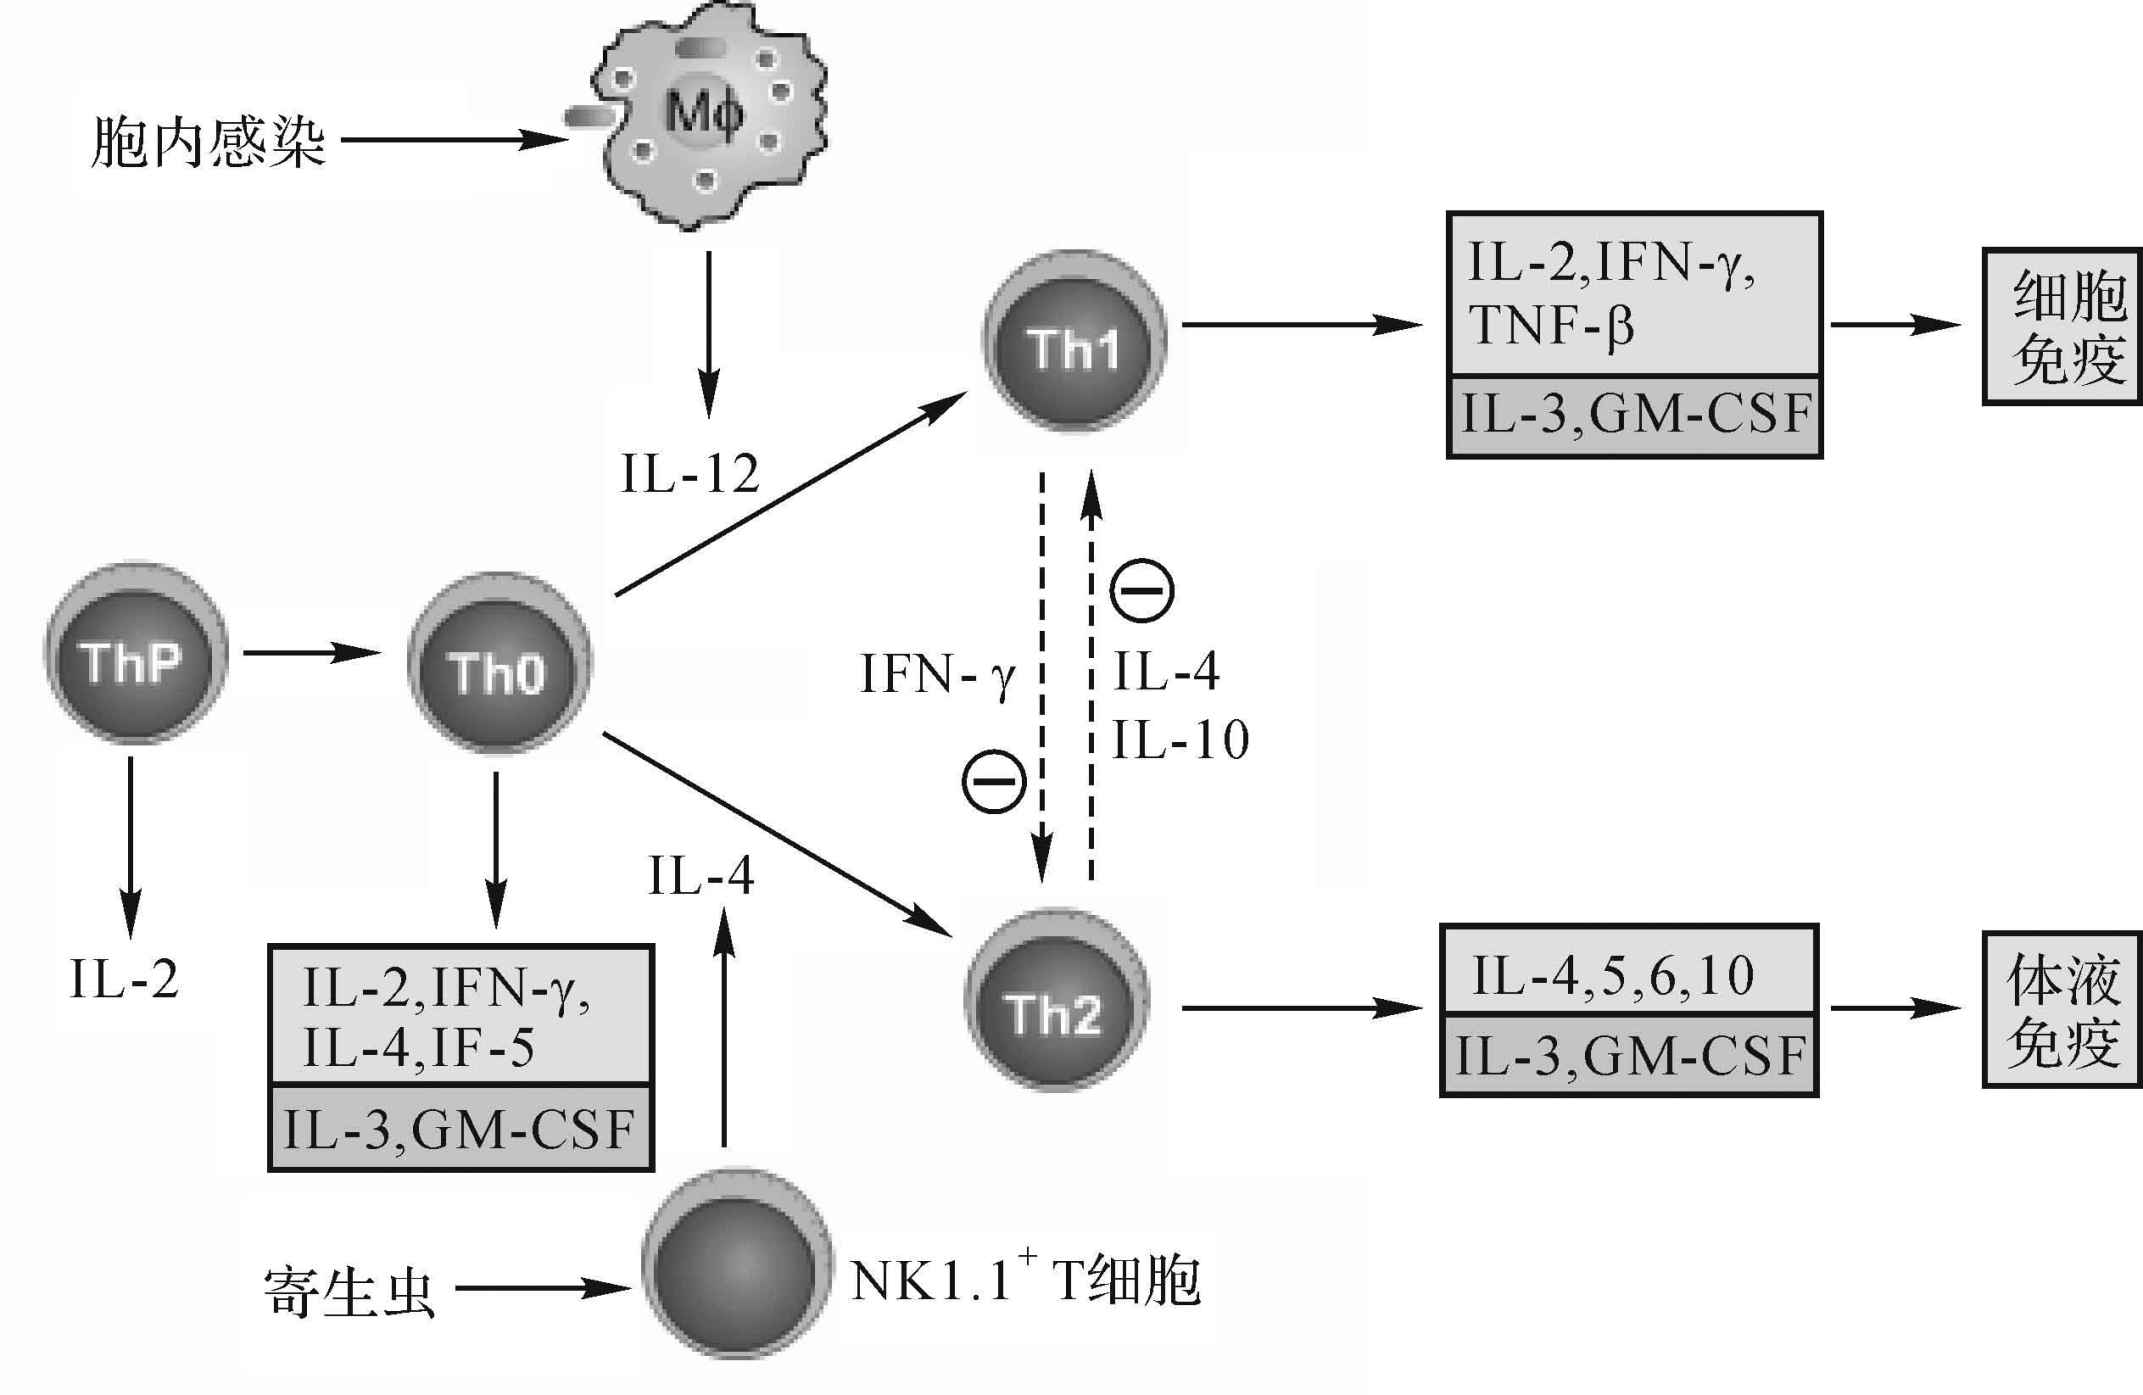
\includegraphics[width=.7\textwidth,height=\textheight,keepaspectratio]{./images/Image00040.jpg}
 \captionsetup{justification=centering}
 \caption{腔隙性脑梗死\\{\small A.病灶位于左侧基底节区和左侧额叶白质区;B.病灶位于脑干}}
 \label{fig2-22}
  \end{figure} 

\textbf{【鉴别诊断】}
脑腔隙在病理上为一脑实质内含水分的<15mm的潜在腔,包括穿支动脉等病变所致的腔隙性脑梗死和非血管病变引起的腔隙病变。发病机制包括血管因素所致的缺血即腔隙性梗死,以及血管因素(如出血、动脉炎等)和血管外因素(如炎症、变性、中毒、机械损伤等)所形成的腔隙性病变,应注意分析。此外,还应注意与前联合及基底节区的扩大的血管周围间隙(多在0.2~1.2cm大小)相鉴别,MR检查有独到鉴别价值。

\subsection{皮质下动脉硬化性脑病}

本病又称Binswanger病,是一组以脑深部小动脉硬化、痴呆、皮质下白质变性、皮质下腔隙或软化为特征的综合征。但有人认为“皮质下动脉硬化性脑病”一词未能正确反映所看到的组织学改变,且过高的估计了临床意义。因此,有关文献应用的非特异性名词较合适,如深部脑白质缺血或老年性白质高信号(MR)。我们认为称为“动脉硬化性脑白质病”或“深部脑白质慢性缺血”更趋合理,同时我们认为有关文献所述及的“脑白质疏松症”亦属本病的范畴。

\textbf{【病因病理】}
主要病因为慢性高血压,其病理特征为弥漫性不完全的皮质下梗死,在侧脑室旁和半卵圆中心的白质内髓鞘肿胀或脱失,皮质下弓状纤维与胼胝体不受累。常有皮质萎缩及皮质下、基底节区腔隙性脑梗死,在髓动脉内有狭窄性动脉粥样硬化。

\textbf{【临床表现】}
见于60岁以上老人,多隐形起病,呈进行性记忆力障碍、严重精神衰退、言语不清,反复发生的神经系统局部体征如偏瘫、失语、偏盲等。病情可缓解和反复加重,常伴有高血压。

\textbf{【CT表现】}
脑白质内斑片状或云絮状稍低密度灶,界限不清,其密度降低不如脑梗死明显。以侧脑室周围分布最明显,其次为半卵圆中心,多为两侧对称性(图\ref{fig2-23})。基底节---内囊区、丘脑、半卵圆中心常伴多发的腔隙性梗死灶,可有脑室系统扩大,脑沟、脑池增宽的弥漫性脑萎缩改变。

\begin{figure}[!htbp]
 \centering
 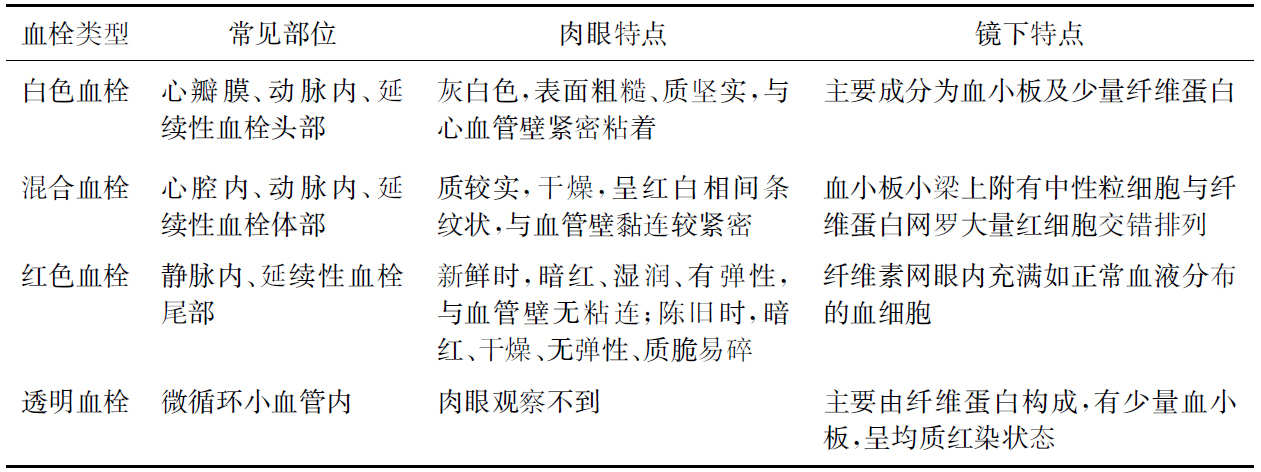
\includegraphics[width=.7\textwidth,height=\textheight,keepaspectratio]{./images/Image00041.jpg}
 \captionsetup{justification=centering}
 \caption{动脉硬化性脑白质病\\{\small 侧脑室周围白质和半卵圆中心区对称性片絮状低密度灶}}
 \label{fig2-23}
  \end{figure} 

\subsection{脑缺氧}

\textbf{【病因病理】}
脑缺氧包括乏氧性缺氧、血液性缺氧、循环性缺氧和中毒性缺氧。常见病因有:高空高原缺氧,呼吸功能不全和某些先心病循环短路、CO中毒以及各种严重贫血、各种休克和心衰,氰化物、硫化氢、磷中毒。脑组织局部循环性缺氧包括颅脑外伤、脑血管意外、脑血流障碍、颅内感染、脑肿瘤急性恶化等。主要病理改变为早期脑组织坏死、水肿,进行性脱髓鞘,晚期脑萎缩。

\textbf{【CT表现】}
①弥漫性脑水肿:以大脑为主,可出现大脑密度普遍减低,而丘脑、脑干和小脑密度相对较高的所谓CT反转征。②局部脑水肿:以脑动脉边缘带(分水岭区)、脑室周围白质最常见,基底节次之,也可见于丘脑和小脑。③缺氧性脑出血:脑实质、脑室周围-脑室、蛛网膜下腔、硬膜下或硬膜外。④脑萎缩:晚期可出现,也可见囊状软化灶。

\subsection{脑静脉窦血栓形成}

颅内静脉血流受阻即脑静脉和静脉窦血栓形成所导致的脑梗死称为静脉性脑梗死,占中风病人的1%~2%。

\textbf{【病因】}
近1/3病因不明。可分为:①全身因素:脱水、糖尿病、高凝血状态、血小板增多症、口服避孕药、妊娠、产后、近期手术、长期应用激素、肾病综合征、心脏病、结缔组织病、新生儿窒息等;②局部因素:局部感染、中耳乳突炎、鼻窦炎、脑膜炎、颅面中耳手术、颅脑外伤、动静脉畸形、动静脉瘘、腰穿等。

\textbf{【临床表现】}
多见于20~35岁女性,其表现各异。头痛最常见,15%急性起病,类似蛛网膜下腔出血,常伴头晕、恶心及视乳头水肿等颅内高压症状。1/3~1/2病人有局灶性神经症状,如颅神经麻痹和意识障碍,半数出现癫痫,还可有偏瘫。小脑静脉血栓可有共济失调等症状。

\textbf{【CT表现】}
最常见于上矢状窦、横窦和乙状窦,其次为海绵窦和直窦。特征性改变为致密静脉征(或索条征)和空三角征,但缺乏特异性。①早期(1~2天):平扫静脉窦内血栓密度与硬脑膜相似,可高达150Hu。增强扫描呈“空三角征”,即三角形的硬膜窦断面,中心不强化而周围强化。②第3~第10天:平扫窦内血块渐吸收,CT值约80Hu左右。③11天后:血凝块基本吸收,窦内CT值约50Hu。④静脉栓塞常伴有弥漫性非对称性脑肿胀、梗死性脑水肿、出血性梗死或单纯出血(脑实质和硬膜下)。静脉性出血其血肿周围界限不清,多靠近脑表面,而且周围环以大片低密度灶有别于动脉性出血。

\textbf{【鉴别诊断】}
高位分叉的上矢状窦、硬膜下脓肿和血肿、蛛网膜下腔出血及窦内窗孔和分隔均可类似空三角征;儿童的流动性静脉血常呈轻度高密度类似血栓,应注意鉴别。

\subsection{高血压脑病}

本病是指在血压迅速剧烈升高时,引起的急性全面性脑功能障碍,属可逆性后部白质脑病综合征(还见于妊娠高血压、慢性肾衰、使用免疫抑制剂和激素等)的范畴。

\textbf{【病因病理】}
可发生于各种原因(原发或继发)引起的动脉性高血压。病理上大多有不同程度的脑水肿,脑表面动脉、静脉和毛细血管扩张,脑切面可见斑点状、裂隙状出血和小动脉壁的坏死。

\textbf{【临床表现】}
该病一般起病急骤,病程短暂,所有症状历时数分钟或1~2小时,最多数天。主要表现为严重头痛、惊厥、偏瘫、失语、黑蒙、神志不清甚至昏迷。

\textbf{【CT表现】}
主要为广泛性脑水肿,呈对称性、弥漫性、边界不清的低密度区,以大脑半球后部最为显著,也可累及小脑。脑室系统变小,脑沟、脑池变浅。血压改善后一段时间随访,完全恢复正常。

\subsection{脑出血}

脑出血是指脑实质内的出血,又称为脑溢血或出血性脑卒中。

\textbf{【病因病理】}
其原因很多,临床上概括为损伤性和非损伤性两大类。后者又称为原发性或自发性脑出血,是指脑内血管病变、坏死、破裂而引起的出血。自发性脑出血绝大多数由高血压和动脉硬化(引起脑小动脉的微型动脉瘤或玻璃样变)所致,其次为脑血管畸形和动脉瘤所致。其他原因还有颅内肿瘤出血、出血性梗死、脑血管淀粉样变、全身出血性疾病、维生素缺乏、新生儿颅内出血、重症肝炎(可合并脑出血、梗死)等。

出血好发于壳核和内囊区(约占50%)、中心部脑白质、丘脑和下丘脑、小脑半球、桥脑,以及脑室内。病理可分为3期:①急性期:血肿内含新鲜血液或血块,周围脑组织有不同程度的水肿,还可有点状出血;②吸收期:血肿内红细胞破坏、血块液化,周围出现吞噬细胞,并逐渐形成含有丰富血管的肉芽组织;③囊变期:坏死组织被清除,缺损部分由胶质细胞及胶原纤维形成瘢痕,血肿小可由此类组织充填,血肿大时则遗留囊腔。

\textbf{【临床表现】}
本病常突然发生剧烈头痛、意识障碍、恶心、呕吐、偏瘫、失语、脑膜刺激征等,按病情发展可分为急性期、亚急性期和慢性期。

临床预后与出血的部位及出血量的多少有关。出血位于皮质下白质区,血肿及水肿引起占位效应,导致出血区功能丧失,但预后相对较好,出血量>30ml为手术指征。小脑或脑干出血压迫四脑室,继发急性颅内压升高,常伴延髓生命中枢损害,直接危及生命,血肿直径>3cm应立即手术。

\textbf{【CT表现】}
血液形成影像的主要成份为含铁的血红蛋白,血液的密度高于脑组织,故CT表现呈高密度。由于脑血管较细,受部分容积效应影响,故血管内血液多不能显示。严重贫血的患者急性期脑出血亦可呈等密度甚至低密度。

\subsubsection{出血量的估计}

一般采用以下公式计算:V(ml)=1/6
π(A×B×C),A为血肿前后径,B为左右径,C为上下径。A、B、C的单位均为厘米。

\subsubsection{CT分期}

通常将脑内血肿分为急性期(1周内)、吸收期(2周~2个月)和囊变期(2个月后)。也有学者根据密度分为:高密度期、等密度期、低密度期、慢性期(图\ref{fig2-24})。

\begin{figure}[!htbp]
 \centering
 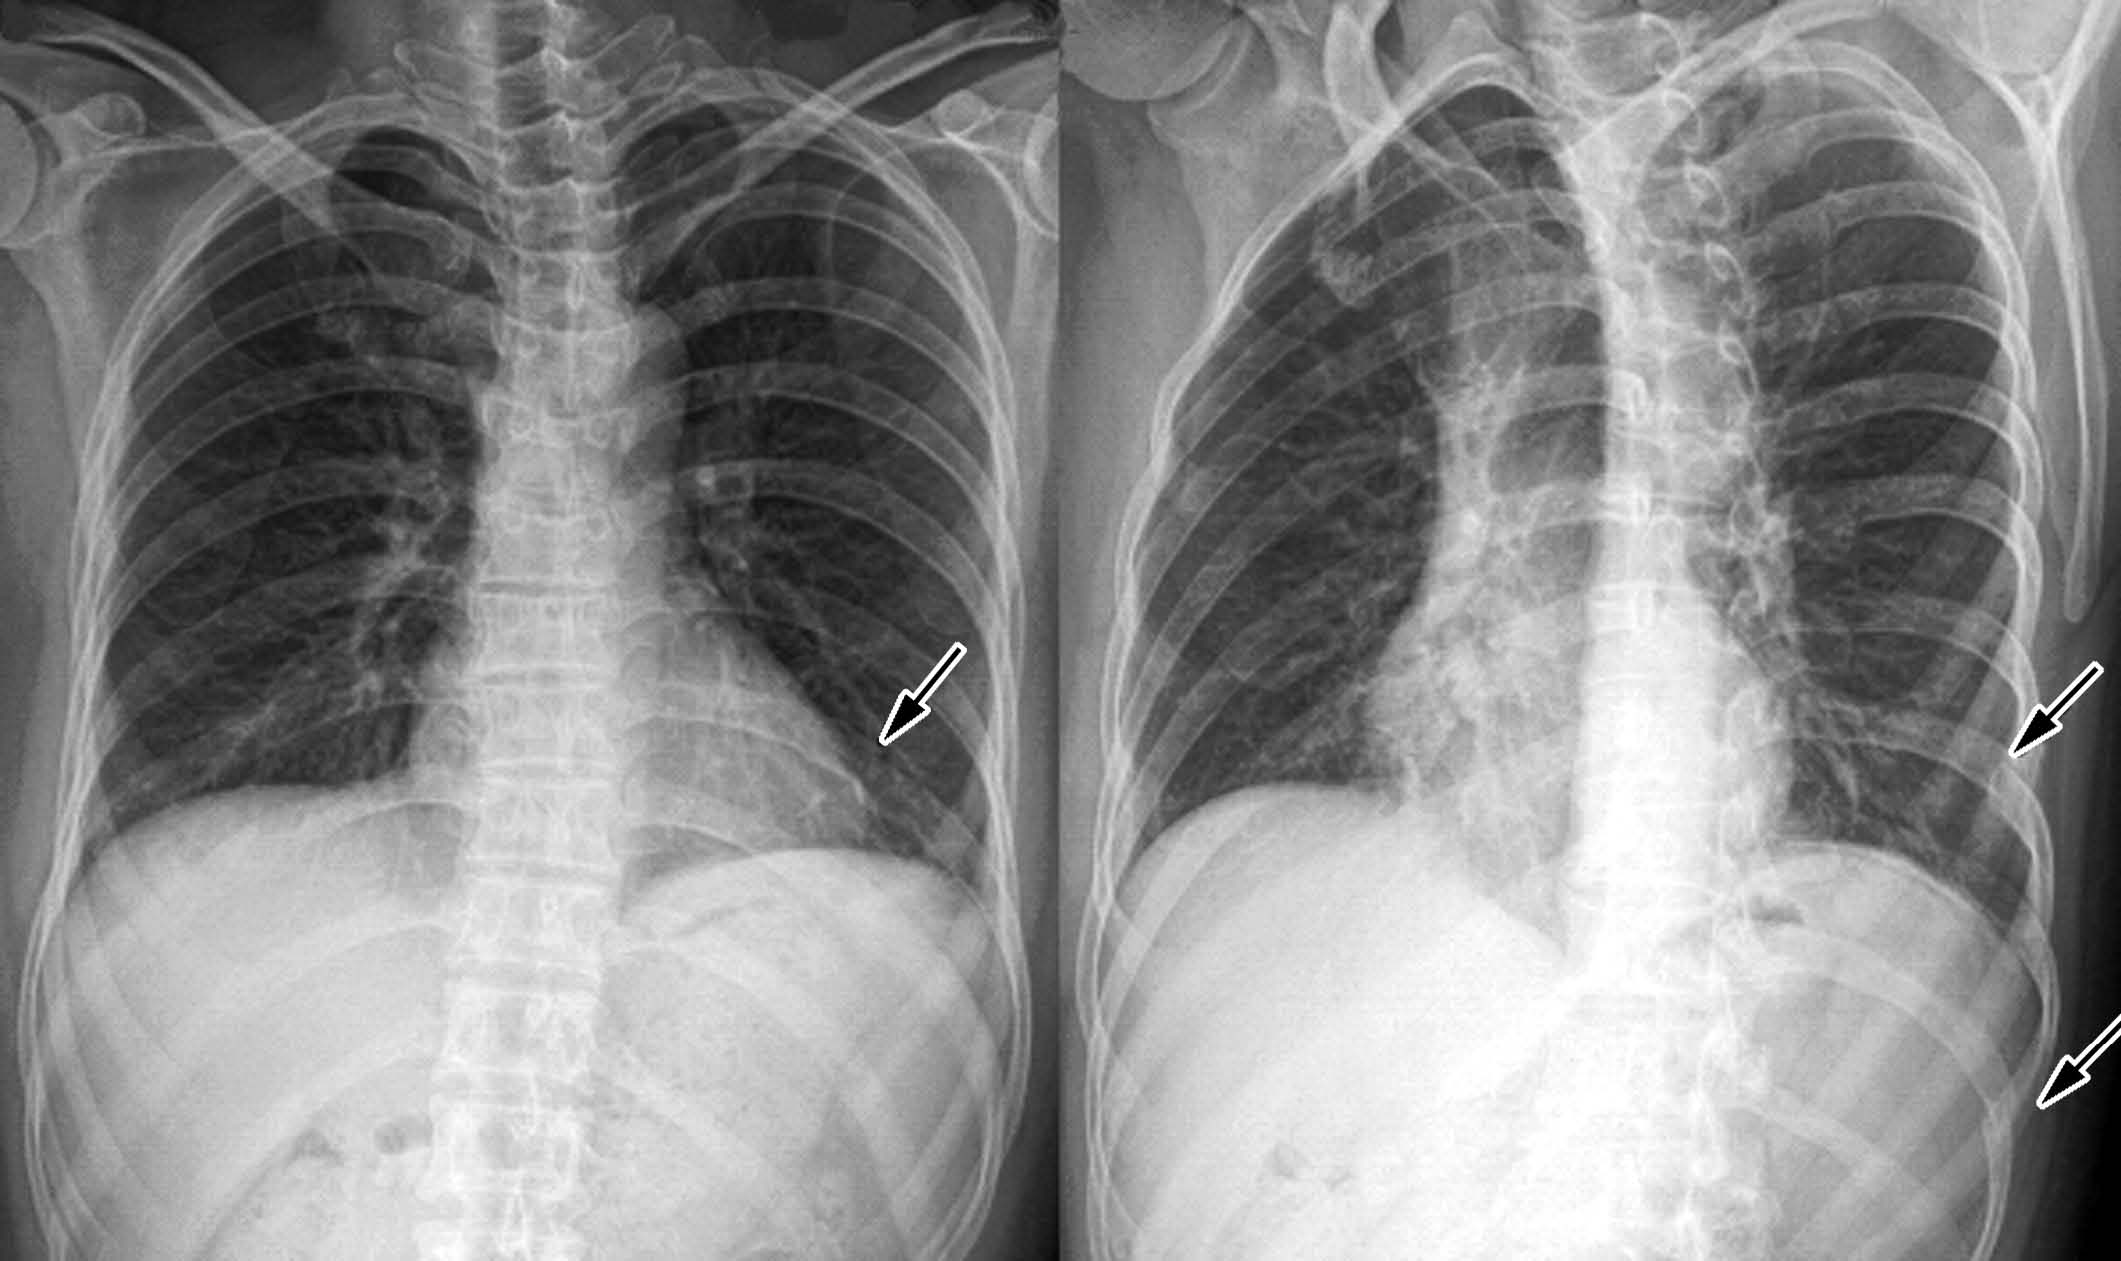
\includegraphics[width=.7\textwidth,height=\textheight,keepaspectratio]{./images/Image00042.jpg}
 \captionsetup{justification=centering}
 \caption{脑出血\\{\small A.右侧丘脑-外囊区血肿破入左右侧脑室内,右外侧裂内亦有血液充填;B.脑出血吸收期,血肿边缘开始吸收呈环状低密度,低密度外可见肉芽组织形成的等密度环}}
 \label{fig2-24}
  \end{figure} 

1.高密度期(1~14天):血液逸出血管后,红细胞分解释放含铁的血红蛋白,表现为高密度区,CT值约50~80Hu。出血3~4天因血液凝固成血块,血浆被吸收,红细胞压积增加,血肿密度达到高峰,甚者达90Hu,周围有水肿。严重贫血者可为等密度,甚至低密度,但血肿有占位征象。

2.等密度期(14~64天):血红蛋白分解,含铁血黄素开始被吸收,血肿呈等密度。但仍有占位效应,水肿仍存在,增强扫描呈环状强化。

3.低密度期(30~84天):血肿周围的新生血管及神经胶质增生形成血肿壁,血肿内含铁血黄素及血红蛋白被吸收,CT呈低密度灶。水肿消失,无占位效应,增强扫描仍呈环状强化。

4.慢性期(3个月后):少量脑出血被胶质和胶原纤维替代而愈合,CT呈略低密度灶。大量脑出血形成囊腔,CT近水样密度,并可出现牵拉现象,增强扫描无或轻微强化。

\subsubsection{脑室内出血}

单纯脑室出血与脑实质内出血破入脑室系统表现一样。少量出血时多沉积在侧脑室后角、第三脑室后部或第四脑室顶部,大量出血常呈脑室“铸型”样表现(图\ref{fig2-25})。早期可有分层现象,以后呈等或低密度,脑室内出血可形成脑积水。

\begin{figure}[!htbp]
 \centering
 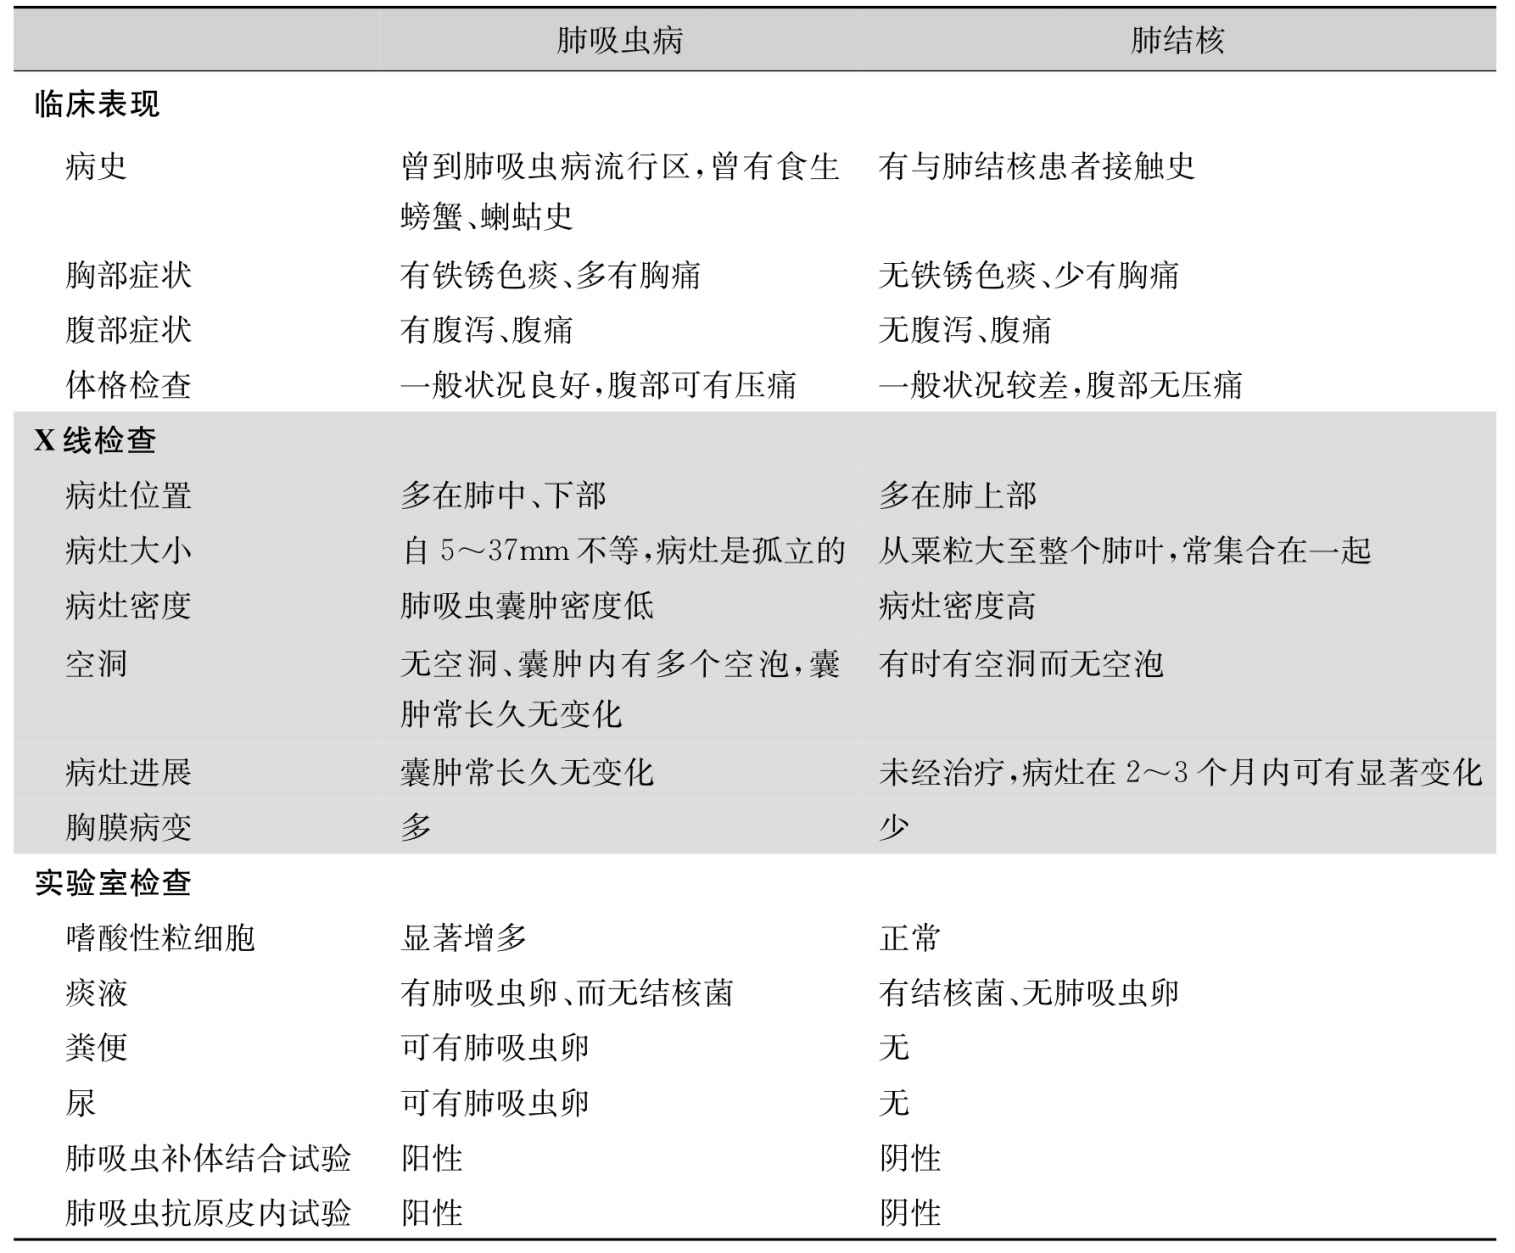
\includegraphics[width=.7\textwidth,height=\textheight,keepaspectratio]{./images/Image00043.jpg}
 \captionsetup{justification=centering}
 \caption{脑室内出血\\{\small 左右侧脑室内有大量血液充填,右侧呈“铸型”样表现}}
 \label{fig2-25}
  \end{figure} 

此外,在诊断时应注意:①急性脑出血大的血肿可形成脑疝。②脑出血可直接破入脑室系统和蛛网膜下腔,亦可由脑室系统进入蛛网膜下腔。③出血周围水肿,在第1天内可出现或表现轻微;3~7天达高峰;出血16天左右占位效应开始减退。④发现灶周水肿与血肿期龄不符时,应考虑肿瘤出血可能。⑤如局部伴有钙化或血肿密度不均等表现,除考虑到肿瘤出血外,也应考虑到脑血管畸形的可能。

\subsection{慢性扩展性脑内血肿}

本病是自发性脑内血肿的一种特殊类型,临床及影像学表现无特异性,易与肿瘤卒中、囊肿合并出血感染等混淆。

\textbf{【病因病理】}
其病因认为与隐匿性血管畸形、血管硬化、外伤、放射损伤、凝血功能障碍有关,一般没有高血压和脑外伤病史。隐匿性血管畸形或微小动脉瘤破裂出血,血肿及其代谢产物不断刺激周围组织产生炎性反应,毛细血管、纤维组织增生,并由增生的毛细血管、纤维组织形成包膜。而其丰富的毛细血管壁脆弱,反复出血、渗出,包膜内液化,使血肿体积逐渐增大。

\textbf{【CT表现】}
多为边缘清楚、密度均匀或不均匀的高、低混杂囊性病灶,且其内可见液-液平面。增强扫描病灶多无强化;部分血肿周围环状强化,为病灶周围脑组织或肉芽组织强化所致。

\subsection{蛛网膜下腔出血}

本病是指颅内血管破裂后血液注入蛛网膜下腔。

\textbf{【病因】}
临床可分为两大类,即外伤性与自发性。自发性原因很多,但以颅内动脉瘤(约占51%)、动静脉畸形(6%)和高血压动脉硬化所致(15%)最多见。此外,20%病因不明。

\textbf{【临床表现】}
自发性常有明显的诱因,如体力劳动过度、咳嗽、用力排便、情绪激动等。绝大多数起病急,剧烈头痛、呕吐、意识障碍、抽搐、脑膜刺激征等,同时可有偏瘫,腰穿有确诊价值。

\textbf{【CT表现】}
一般在出血3天内检出率最高,可达80%~100%,一周后很难检出。特征性表现为基底池、侧裂池和脑沟内等广泛的高密度影(图\ref{fig2-26})。如出血量少或严重贫血均不易发现。大脑前动脉破裂血液多积聚于视交叉池、纵裂前部;大脑中动脉破裂血液多积聚于一侧的外侧裂附近,也可向内流;颈内动脉破裂血液也以大脑外侧裂为多;椎基动脉破裂血液主要积聚于脚间池和环池。但出血量大者可难以估计出血部位。

\begin{figure}[!htbp]
 \centering
 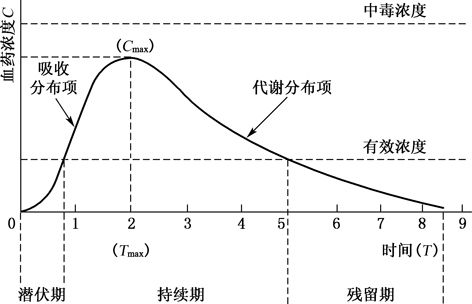
\includegraphics[width=.7\textwidth,height=\textheight,keepaspectratio]{./images/Image00044.jpg}
 \captionsetup{justification=centering}
 \caption{蛛网膜下腔出血\\{\small A、B为同一患者,鞍上池、左右外侧裂池、纵裂池前部、环池、四叠体池、大脑大静脉池内均有大量高密度血液充填}}
 \label{fig2-26}
  \end{figure} 

\textbf{【并发症】}
①脑积水:脑积水早期为梗阻性,发生率约为20%。可演变成交通性。②脑动脉痉挛:造成脑缺血和脑梗死,发生率约25%~42%。③伴发脑内血肿和(或)硬膜下血肿、脑室内出血:常与动脉瘤、动静脉畸形或脑肿瘤出血有关。

\subsection{颅内动脉瘤}

动脉壁呈局限性病理性扩张,与动脉腔有一颈部相连。

\textbf{【病因病理】}
其病因有先天性因素、动脉粥样硬化、感染因素和外伤4个方面。根据影像学可分为5种病理类型:①粟粒状动脉瘤;②囊状动脉瘤;③假性动脉瘤;④梭形动脉瘤;⑤壁间动脉瘤。

\textbf{【临床表现】}
好发于20~70岁。在破裂前90%无特殊临床症状,少数可影响到邻近神经或脑结构而产生症状。破裂后引起蛛网膜下腔出血和颅内血肿而出现相应的症状体征。

\textbf{【CT表现】}
颅内动脉瘤好发于脑动脉,约90%~95%分布于颈内动脉系统,5%~10%分布于椎动脉系统。颈内动脉瘤约占20%~40%,大脑中动脉瘤约占21%~31%,前交通及大脑前动脉瘤约占30%~37%,多发性约占4%~5%。

1.颅底较小动脉瘤:平扫难以显示,增强扫描呈高密度。

2.较大动脉瘤:平扫呈圆形等或高密度,边缘光整,有时瘤壁可见钙化。增强扫描呈均匀强化,而血栓无强化。

3.巨大动脉瘤:即直径>2.5cm的动脉瘤,其CT表现可分3型。①无血栓形成型:平扫呈圆形或椭圆形等或略高密度,瘤壁钙化较其他类型少见。增强扫描均匀强化。②部分血栓形成型:最常见,呈圆形或卵圆形略高密度,壁多有弧形钙化。增强扫描流动的血液强化明显,血栓不强化,从而形成高密度影内的低密度点称为“靶征”。周围很少有水肿。③完全栓塞型:平扫为圆形或卵圆形混杂略高密度,瘤壁常有钙化,周围无水肿。增强扫描呈环状强化。

此外,CTA显示动脉瘤的敏感性可达95%,特异性近83%。

\textbf{【并发症】}
①颅内出血:蛛网膜下腔出血、脑内血肿和脑室内积血,甚至可穿破蛛网膜造成硬膜下血肿。②脑血管痉挛:蛛网膜下腔出血所致,并导致相应区域的水肿、梗死。③脑积水:蛛网膜下腔出血所致。

\textbf{【鉴别诊断】}
动脉瘤周围多无水肿,瘤壁可有环形强化,动态CT扫描时间-密度曲线呈速生速降型,与血管相同。而肿瘤则表现为缓慢上升和下降的时间-密度曲线是鉴别的关键。

\subsection{脑动静脉畸形}

脑血管畸形分为5型:①动静脉畸形(AVM);②海绵状血管瘤;③静脉畸形(又称静脉血管瘤);④毛细血管扩张症(又称毛细血管瘤,以MR诊断为佳);⑤血管曲张(包括大脑大静脉畸形等)。其中AVM最常见,约占90%以上。毛细血管扩张症一般只被病理诊断,CT或MR很难显示,偶见钙化。

AVM是最常见的血管畸形,但有相当一部分脑血管造影阴性,称为隐匿性AVM。

\textbf{【病理】}
AVM由一条或多条供血动脉、畸形血管团、一条或多条引出静脉组成。常见于大脑中动脉分布区的脑皮质,亦可发生于侧脑室(如脉络丛)、硬脑膜、软脑膜、脑干和小脑。

\textbf{【临床表现】}
好发于20~30岁,男性多于女性,10%~15%无症状。常见的症状有:①头痛:偏头痛或全头痛,阵发性;②出血:出现相应症状和体征;③癫痫:约30%为此就诊;④脑缺血症状:脑梗死、脑萎缩;⑤部分颅外听到杂音。

\textbf{【CT表现】}
AVM平扫呈局灶性高、低或低、等混杂密度区,多呈团块状,也可见点、线状影,边缘不清,但有时可不显示。常伴斑点状或条状钙化,轻度或无占位征象。病灶周围无水肿表现,但有时可出现脑室扩大和交通性脑积水。增强扫描呈团块状强化,有时可见迂曲的血管影,造影剂充盈及排出均较快。CTA多可有效显示其供血动脉、畸形血管团和引流静脉(图\ref{fig2-27})。



\begin{figure}[!htbp]
 \centering
 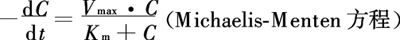
\includegraphics[width=\textwidth,height=\textheight,keepaspectratio]{./images/Image00045.jpg}
 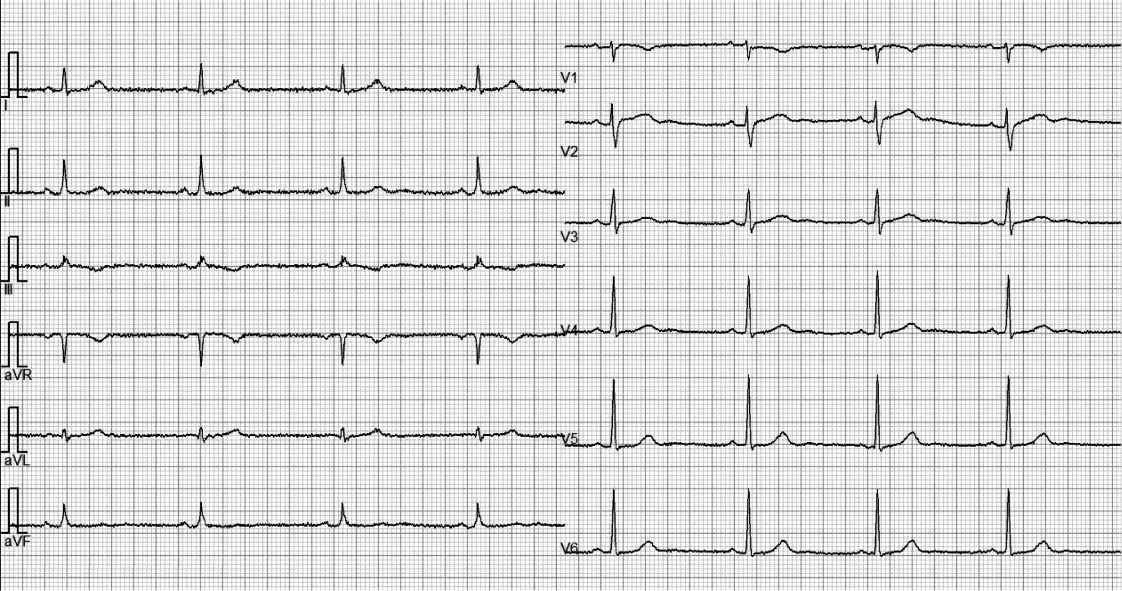
\includegraphics[width=\textwidth,height=\textheight,keepaspectratio]{./images/Image00046.jpg}
 \captionsetup{justification=centering}
 \caption{脑动静脉畸形\\{\small A~D为同一患者,平扫(A、B图)左侧颞叶有局灶性高、等混杂密度区,形态不规则,其边缘有蚯蚓状高密度影(引流静脉);增强扫描(C图)呈团块状强化,并见迂曲的引流静脉影;CTA(D图)清晰显示畸形血管团和粗大的引流静脉}}
 \label{fig2-27}
  \end{figure} 

其并发症有出血、梗死、软化灶及局限脑萎缩表现。

\textbf{【鉴别诊断】}
钙化明显的肿瘤以及强化明显的肿瘤(如胶质瘤)其水肿及占位效应均较显著,可与AVM鉴别。AVM增强扫描的时间-密度曲线与血管相似亦是与肿瘤鉴别的重要依据。

\subsection{颅内海绵状血管瘤}

本病占脑血管疾病的7%,近年来的研究显示其属不完全染色体显性遗传性疾病。目前多认为其发生源于脑内毛细血管水平的血管畸形,可位于脑内或脑外,为非真性肿瘤。

\textbf{【病理】}
病灶由微动脉延伸出来的、血流缓慢的、大小不等的丛状薄壁的血管窦样结构组成,其间有神经纤维分隔,窦间没有正常脑组织。由于其血管壁薄而缺乏弹性,且易于发生玻璃样变、纤维化,因而易出血,并可有胶质增生、坏死囊变、钙化,病灶可全部钙化形成“脑石”。病灶周围可见含铁血黄素沉着或有机化的血块。病灶无明显的供血动脉及引流静脉。

\textbf{【临床症状】}
好发于40~60岁,常以颅内出血为首发症状。典型表现为癫痫发作、突发性头痛和进行性神经功能障碍等。

\textbf{【CT表现】}
80%位于幕上,好发于额、颞叶,也可发生于蛛网膜下、硬膜下,脑外者多位于鞍旁海绵窦区。多表现为界限清楚的圆形或卵圆形的等至稍高密度影(图\ref{fig2-28})。其内可见“颗粒征”颇有特征,即在略高密度背景内含有数量不一的颗粒状高密度影和低密度影,前者为钙化,后者为血栓形成。除急性出血或较大病灶,灶周一般无水肿及占位征象。可能因为供血动脉太细或已有栓塞,也可能因病灶内血管床太大,血流缓慢使对比剂稀释,致使增强扫描不强化或仅见周边强化。其强化程度取决于病灶内血栓形成和钙化的程度,血栓形成轻、钙化不明显者强化明显。国外报道脑外者可有骨侵蚀。

\begin{figure}[!htbp]
 \centering
 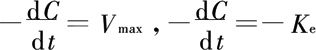
\includegraphics[width=.7\textwidth,height=\textheight,keepaspectratio]{./images/Image00047.jpg}
 \captionsetup{justification=centering}
 \caption{颅内海绵状血管瘤\\{\small A、B非同一患者,A示病灶位于小脑左侧半球,B示病灶位于脑干;病灶均呈近圆形稍高密度灶,周围无水肿}}
 \label{fig2-28}
  \end{figure} 

\textbf{【鉴别诊断】}
①主要应与脑膜瘤鉴别。后者平扫密度多均匀一致,增强扫描明显强化,常有明显占位征象,并可出现水肿征象及颅骨增生和吸收有助鉴别。②少数血管瘤呈环状并伴壁结节,偶有出血,病灶内显示血-液平面伴周围水肿,不易与胶质瘤等相鉴别。

\subsection{脑静脉性血管畸形}

本病又称脑静脉性血管瘤、脑发育性静脉异常,是一种组织学上由许多扩张的髓静脉和一条或多条引流静脉组成的血管畸形。国外有学者认为是一种正常引流静脉的非病理性变异。

\textbf{【病因病理】}
其病因不明,多认为是胚胎发育时宫内意外因素导致静脉阻塞,由侧支代偿所致。其形成时间在脑动脉形成之后,故仅含静脉成分。畸形血管由许多扩张的放射状排列的髓静脉汇入一条或多条引流静脉组成,向皮质表面和静脉窦或向室管膜下引流,可分为皮层表浅型、皮层下型和脑室旁型。

\textbf{【临床表现】}
好发于35~40岁,男女发病率相近。一般无症状,少数可产生癫痫、头痛,出血者可有感觉和运动障碍、共济失调等。

\textbf{【CT表现】}
它可发生在脑静脉系统的任何部位,但以额叶侧脑室前角附近的髓质区和小脑深部髓质区最常见,其次为顶叶、颞叶和脑干。

CT平扫阳性率不到50%。最常见的表现为圆形高密度影(34%),系扩张的髓静脉网,无水肿和占位效应,可见高密度的含铁血黄素沉着或钙化。

增强扫描阳性率为87%,可见3种表现:①白质中圆形强化影(32.5%),系髓静脉网或引流静脉;②穿越脑的线形增强影(32.5%),为引流静脉;③两者同时出现(18.6%)。

特征性表现是三维CT血管造影(CTA)静脉期脑静脉成像(CTV)出现“海蛇头”样的深部髓静脉汇集到单根粗大的引流静脉,然后汇入到表浅的表层静脉或硬膜窦等征象。但发生于脑室壁上者“海蛇头”征象不明显。

\subsection{Galen静脉瘤}

本病又称大脑大静脉扩张、大脑大静脉瘘、大脑大静脉畸形等。

\textbf{【病因病理】}
本病是由于动静脉短路,流入Galen静脉(即大脑大静脉)内的血流增多引起局部管腔扩张。这些短路血管多来源于颈内动脉系统或基底动脉系统,多异常扩大迂曲。静脉窦闭塞引起大脑大静脉回流受阻也是其重要的致病原因。压迫中脑导水管可致脑积水。

\textbf{【临床表现】}
在新生儿、幼儿中常因动脉血直接进入静脉造成心功能不全。脑积水后可出现头痛、痉挛性抽搐、颅内压增高等症状。

\textbf{【CT表现】}
平扫可见第三脑室后部中线处之大脑大静脉池区等密度或高密度的圆形肿块,病灶边缘多光滑,与窦汇之间有扩张的直窦相连为特异性表现。可伴有病灶边缘钙化、局部脑萎缩、血肿或脑积水。增强扫描病灶呈均匀性强化,偶可显示强化的供血动脉和引流静脉。

\subsection{颈动脉海绵窦瘘}

本病是指颈动脉及其分支与海绵窦之间异常沟通所致的一组临床综合征。海绵窦为中颅凹两层硬脑膜构成的硬脑膜窦,眼上静脉、眼下静脉、蝶顶窦静脉、外侧裂静脉和基底静脉汇入其中,颈动脉穿行其间。这是体内惟一动脉通过静脉的结构。当任何原因造成颈内动脉壁破裂后,动脉血直接流入海绵窦,就形成海绵窦区动静脉瘘。

\textbf{【病因】}
病因分为两大类:①外伤性:多见,大多由颅底骨折所致;②自发性:病因较多,主要见于颈内动脉虹吸部动脉瘤破裂、硬膜型动静脉畸形及遗传性胶原纤维缺乏病等。此外,动脉硬化、炎症、妊娠等也可造成自发性。根据解剖部位分为颈动脉海绵窦瘘和硬脑膜动脉海绵窦瘘,前者多为外伤性,后者多为自发性。

\textbf{【临床表现】}
头痛、癫痫、耳鸣、视力障碍、搏动性突眼、眼球运动障碍、颅内杂音,甚至因颅内出血而出现相应症状。

\textbf{【CT表现】}
①患侧海绵窦扩大,密度增高;②眼上静脉增粗;③眼球突出;④增强示扩大的海绵窦及迂曲的眼上静脉显著强化(图\ref{fig3-8},见第三章)。此外,眼外肌肥厚和眶内软组织肿胀、突眼,患侧脑组织水肿、出血、萎缩是引流静脉压力增高及“盗血”引起的继发改变。

\subsection{颅骨膜血窦}

本病又称血囊肿、局限性静脉曲张或骨血管瘤,是指紧贴颅骨外板的扩张静脉,它们穿过颅骨的板障静脉与硬膜窦相交通。

\textbf{【病因】}
其原因不明,可由先天性、自发性或外伤性所致。有学者认为外伤是本病的最主要因素。

\textbf{【临床表现】}
多见于儿童,通常以头皮肿块就诊。头皮中质软的膨隆性肿块,无搏动,局部皮肤可以微红或青紫色。通常位于中线部位,偶尔位于侧旁,以额部为主,偶有头痛、恶心、乏力等。肿块随颅内压力的变化而改变其大小,即平卧或头低时肿块增大为其特征性症状。

\textbf{【CT表现】}
大多位于颅外中线部位或附近,上矢状窦近端,以额、顶部多见。表现为颅外头皮下均匀的软组织密度肿块,边缘清晰,无钙化,随体位大小可变化。颅外板可有轻度压迹,颅骨内有孔状骨质缺损。增强扫描静脉窦内对比剂可通过颅骨的缺损弥散至囊腔内,呈均匀或不均匀显著强化。

\subsection{颅内血管延长症}

本病是指颈内动脉及椎基底动脉有规律的直径增大和普遍而有规律的延长为特征的血管异常。颈内动脉及椎基动脉的延长属于一种少见的先天性血管壁异常。

\textbf{【病理】}
延长的血管均伴有不同程度的动脉粥样硬化、弹性内膜的破坏及其肌壁的纤维化,最终导致血栓形成或栓塞。

\textbf{【临床表现】}
其发病特点主要取决于受累血管的范围、病变大小及所压迫的邻近组织情况。基本分为3类:①脑血管意外;②颅神经受压症状:如Ⅲ、Ⅴ~Ⅷ颅神经受压;③占位效应对脑组织功能的影响:如痴呆、共济失调、震颤麻痹等,也有阻塞性脑积水的可能。

\textbf{【CT表现】}
本病所涉及的血管有基底动脉、颈内动脉幕上段、大脑中动脉、大脑后动脉。CTA可发现异常扭曲扩张的颈内或基底动脉段,管壁可钙化。其中,基底动脉病变的诊断标准为上段基底动脉的直径增大达4.5mm和基底动脉上段超过床突平面6mm以上,且延长的血管可伴有迂曲移位和血管袢形成。

\subsection{烟雾病}

本病又称Moyamoya病、脑底动脉环闭塞、脑底异常血管网症等,是一种脑动脉进行性狭窄、闭塞性疾病。

\textbf{【病因】}
其病因不明,凡能引起颈内动脉末端、大脑前动脉和大脑中动脉近端慢性进行性闭塞的先天因素(发育不良)或后天因素(外伤、感染、动脉硬化)均可导致本病。近来遗传因素受到重视。

\textbf{【临床表现】}
以10岁以前儿童多见,亦可见于成人。主要有缺血性和出血性两大类表现。脑血管造影是确诊的主要手段。

\textbf{【血管造影】}
特点为:①大脑前、中动脉起始处狭窄或闭塞;②脑底异常血管网形成;③侧支循环广泛建立;④两侧颞、额、顶叶、基底节区梗死或出血。本病即因造影时异常血管网和侧支循环的显影似烟雾状而得名。

\textbf{【CT表现】}
无特异性。①脑梗死、软化灶:常见于颞、额、顶叶,很少见于基底节,小脑、脑干不发生。②脑萎缩:多为双侧性,额叶为甚,脑室扩大以侧脑室和第三脑室显著。③出血灶:可为脑内或蛛网膜下腔。④颅底、基底节区有点状、迂曲、不规则的网状影,并可见强化。

\section{颅脑外伤及其他损害}

\subsection{头皮损伤}

颅盖软组织在额、顶、枕部分为皮肤、皮下组织、帽状腱膜、帽状腱膜下层和颅骨骨膜5层。前3层紧密连接CT不能识别。帽状腱膜下层由疏松结缔组织构成,内含少量血管,CT呈低密度带。而在颞部则由皮肤、皮下组织、颞浅筋膜、颞深筋膜、颞肌和颅骨骨膜6层构成。

头皮损伤包括:①头皮血肿或称颅外血肿,包括位于头皮与帽状腱膜间的皮下血肿、帽状腱膜下血肿(图\ref{fig2-29})和骨膜下血肿;②头皮撕裂伤、擦伤和挫伤等。

\begin{figure}[!htbp]
 \centering
 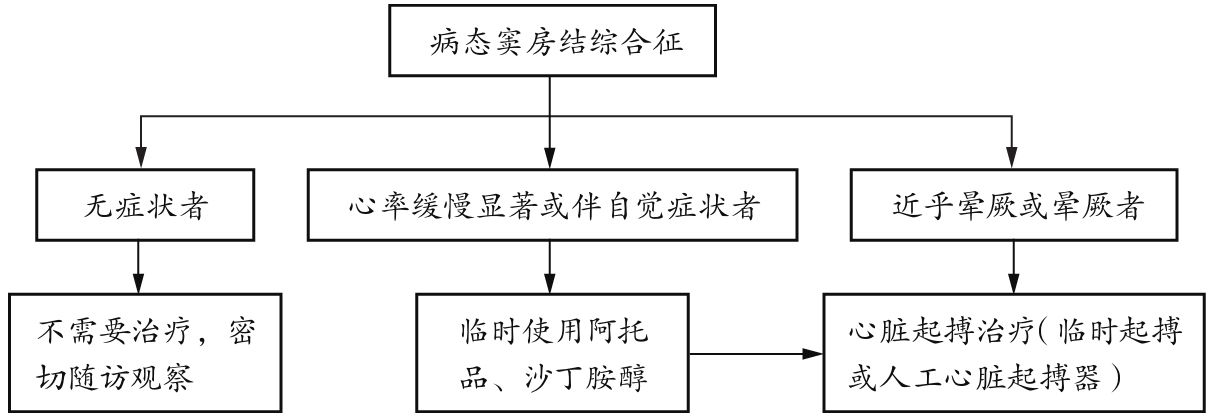
\includegraphics[width=.7\textwidth,height=\textheight,keepaspectratio]{./images/Image00048.jpg}
 \captionsetup{justification=centering}
 \caption{帽状腱膜下血肿\\{\small 出血位于左侧额顶枕部帽状腱膜下}}
 \label{fig2-29}
  \end{figure} 

头皮血肿多由于头皮血管破裂引起,也可因板障静脉或硬脑膜血管破裂,血液沿骨折缝聚集于骨膜下,后者多伴硬膜外血肿。

\subsection{颅骨骨膜下血肿}

骨膜下血肿是颅外血肿的少见类型。

\textbf{【病因病理】}
多发生于新生儿产伤和婴幼儿头部外伤。血肿位于颅骨外板与对应的骨膜之间的潜在腔隙,好发于顶骨,其次为枕骨。

\textbf{【临床表现】}
产伤所致者几乎均因头皮下出现软组织包块,未消散且逐渐变硬而就诊。

\textbf{【CT表现】}
特征性表现是新鲜血肿范围达到受累骨的整个表面,中止于颅缝或不跨越颅缝,边缘清楚锐利。而头皮下及帽状腱膜下血肿不受颅缝限制有助于鉴别。2~3周后血肿包膜出现弧形、壳状钙化,从边缘开始逐渐形成一个完整的包壳,这一过程大约需要3~6个月。与此同时血肿逐渐吸收机化,血肿完全机化约需1年,此时血肿包膜钙化或骨化形似颅骨外板,血肿机化钙化形似板障。再经过长期的塑形与颅骨融合,致局部颅骨增厚、外突隆起,并可成为永久性后遗表现。

此外,少数在血肿部位出现或大或小的囊状骨缺损,可持续数年或更久。与颅骨表皮样囊肿、嗜酸性肉芽肿、韩雪柯氏病相类似,应注意鉴别。

\subsection{颅骨骨折}

1.按骨折形态分类:①线状骨折。②凹陷骨折:婴幼儿颅骨质软,骨折部位凹陷,但不出现骨折线,称为乒乓球样凹陷骨折。③粉碎性骨折:大多数凹陷骨折被分离为多个骨碎块,则被称为粉碎性骨折。④穿通骨折:多为锐器直接损伤,少数为火器伤。局部头皮全层裂伤,可有各种类型骨折,还可见颅内血肿、异物及脑损伤。⑤颅缝分离:两侧不对称或颅缝宽>2mm。

2.按骨折部位分类:①颅盖骨骨折。②颅底骨折。

3.诊断骨折应注意的问题:①颅骨血管沟:仅有内板压迹,边缘为硬化边。②板障静脉:常不规则,可见于对侧,并终端于静脉湖。③颅骨缝:特有的部位及走行,是区别骨折线的标志。④是否有颅内积气:积气可见于蛛网膜下腔、脑室系统、硬膜下腔,以及硬膜外血肿内,甚至脑实质内。

\subsection{硬脑膜外血肿}

硬脑膜紧贴颅骨内板,当颅骨骨折或脑膜血管破裂、出血使其与颅内板分离时则形成硬膜外血肿。

\textbf{【病理】} 多发生于头颅直接损伤的部位。约
95%伴颅骨骨折,70%~80%病例因骨折所致脑膜中动脉及其分支断裂,少数因骨折伤及板障静脉、静脉窦和蛛网膜粒。血肿可单发或多发,呈凸透镜形,多不伴有脑实质损伤。

\textbf{【临床表现】}
伤后有短时原发昏迷,清醒后头痛、呕吐逐渐加重并再度昏迷。清醒时间的长短,由出血量多少和出血速度决定。重者如不及时处理,可形成脑疝。

\textbf{【CT表现】}
因硬膜与颅骨紧密相连,故血肿局限呈梭形高密度,CT值为50~70Hu。血肿的脑侧缘光滑(图\ref{fig2-30}),好发于骨折处。由于硬膜在颅缝处与骨结合紧密,故血肿不超越颅缝。但骨折如跨越颅缝,则血肿亦可跨越颅缝,也可从幕上延及幕下或跨越中线。血肿有占位效应,但较硬膜下血肿轻,多不伴脑实质损伤,但压迫邻近血管时可发生脑水肿或脑梗死。少数受伤时无症状,以后才发生慢性硬膜外血肿。慢性硬膜外血肿其壁机化增厚并可钙化。

\begin{figure}[!htbp]
 \centering
 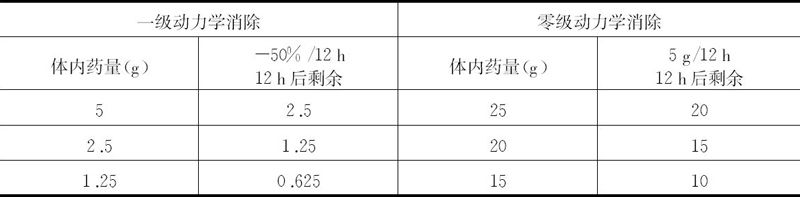
\includegraphics[width=.7\textwidth,height=\textheight,keepaspectratio]{./images/Image00049.jpg}
 \captionsetup{justification=centering}
 \caption{硬膜外血肿\\{\small 右侧颅骨内板下有梭形高密度区,边缘清晰锐利}}
 \label{fig2-30}
  \end{figure} 

\subsection{硬脑膜下血肿}

硬膜下血肿位于硬膜和蛛网膜之间,多因减速性挫伤(对冲伤)所致,无颅骨骨折或骨折仅位于暴力部位。

\textbf{【病理】}
其血源多为脑对冲伤处的静脉、小动脉或由大脑向上矢状窦汇入的桥静脉撕裂所致。呈新月形包绕在大脑表面,在伤后不同时间形态变化各异,约50%合并脑挫裂伤。临床、病理和影像均分为急性、亚急性和慢性3期。

CT上等密度硬膜下血肿占硬膜下血肿的16%。据有关文献报道,多发生在初次损伤后30~90天,亦有报道可达120天,甚至150余天。等密度硬膜下血肿的原因为:①血肿由高密度向低密度发展过程中血肿密度与脑组织密度相近时;②偶有低蛋白血症(如贫血)病人的急性期血肿呈等密度;③再出血或慢性出血进入到慢性硬膜下血肿,而形成等密度慢性硬膜下血肿。

\textbf{【临床表现】}
急性者病情多较重,且发展迅速,出现中间清醒期或意识好转期者较少,颅内压增高、脑受压和脑疝症状出现早。慢性硬膜下血肿患者年龄常较大,只有轻微外伤史,在伤后数周或数月出现颅内压增高症状,呈慢性过程。

\textbf{【CT表现】}

\subsubsection{三期表现}

1.急性期:伤后3天内。一般呈均匀高密度的新月形(图\ref{fig2-31}A),血肿可跨颅缝,但不超过中线。占位效应著,常伴脑挫裂伤,可形成脑疝。有3种非典型表现:①血肿密度不均:可能与急性出血还未凝固、凝血早期血清外溢或蛛网膜破裂脑脊液进入硬膜下有关;②血肿呈梭形表现:可能与出血没有及时散开有关;③血肿同侧侧脑室扩大:可能与同侧室间孔被迅速挤压梗阻所致。

此外,多不伴骨折,但骨折后硬膜撕裂也可形成急性硬膜下血肿。

2.亚急性期:伤后4天~3周内。血肿可逐渐变为等密度,而表现为皮质区均匀受压,脑沟消失,灰白质交界处被均匀向内推移。但双侧均有血肿,中线推移可不著。亚急性血肿的较早期出现细胞沉淀效应可出现密度上低下高的液体界面。

3.慢性期:伤3周后。此时血肿包膜形成,凝血块液化,逐渐变成液性低密度(图\ref{fig2-31}B),血肿壁机化增厚或钙化。血肿内肉芽组织增生、机化形成包膜,故可见慢性硬膜下血肿有分隔表现。

\subsubsection{等密度硬膜下血肿}

平扫表现为中线结构及脑室受压移位、变形,脑沟、裂池变窄消失、灰白质界面内移等,均属间接征象(图\ref{fig2-31}C)。增强扫描可显示血肿的位置、大小、形态而确诊。



\begin{figure}[!htbp]
 \centering
 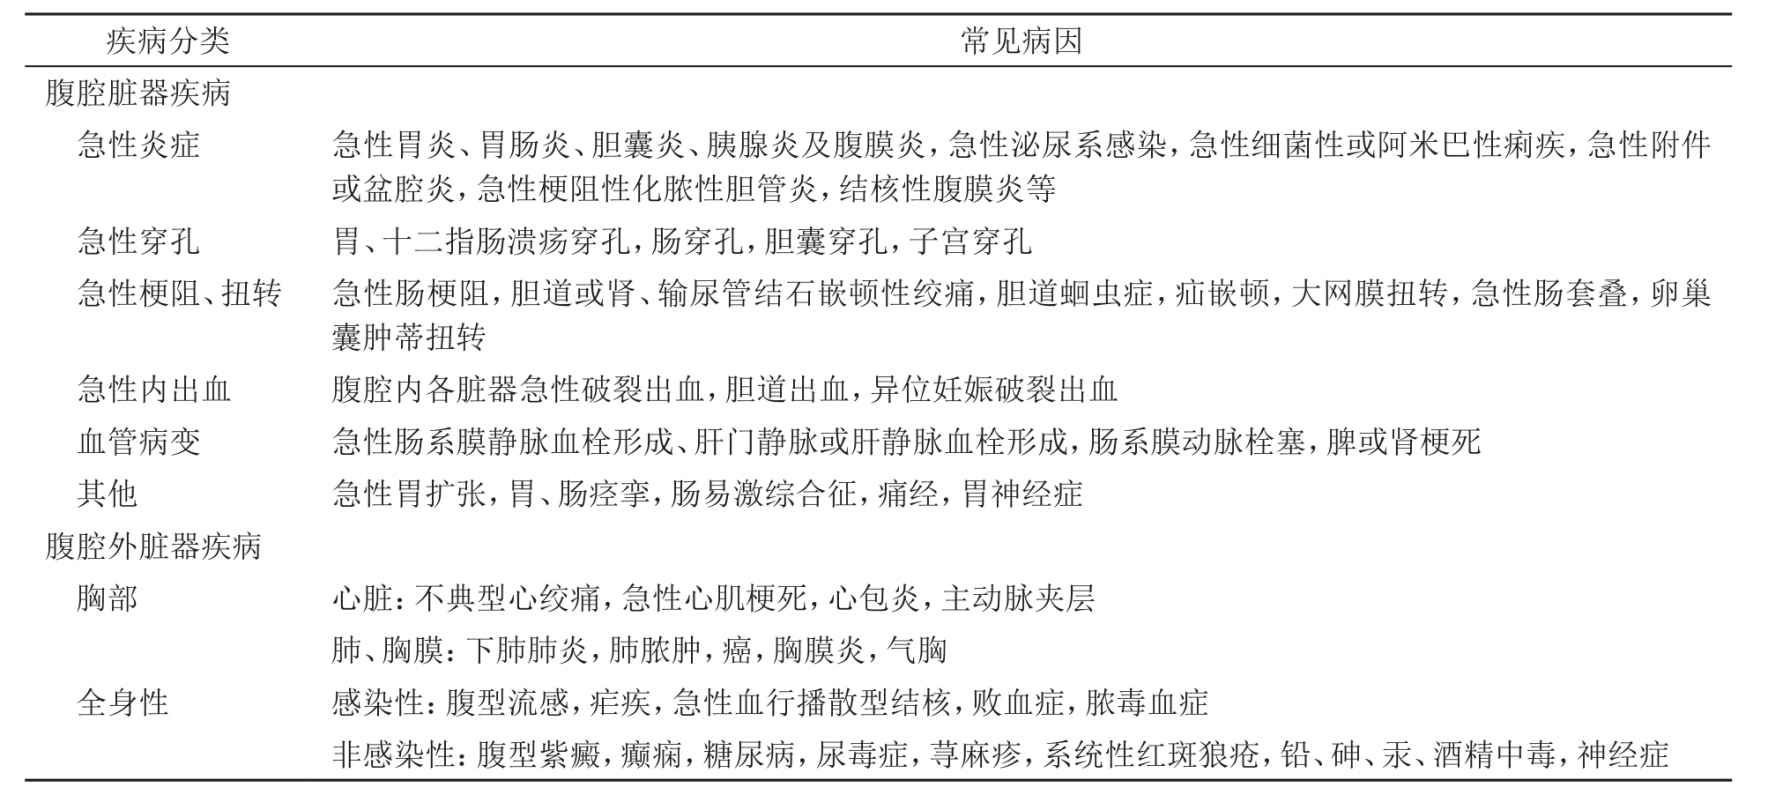
\includegraphics[width=.7\textwidth,height=\textheight,keepaspectratio]{./images/Image00050.jpg}
 \includegraphics[width=.7\textwidth,height=\textheight,keepaspectratio]{./images/Image00051.jpg}
 \captionsetup{justification=centering}
 \caption{硬膜下血肿\\{\small A.急性期硬膜下血肿,病灶位于左侧额顶骨内板下;B.慢性期硬膜下血肿,病灶位于左侧额顶枕骨内板下,有密度上低下高的液体界面;C.慢性等密度硬膜下血肿,病灶位于左侧额顶枕骨内板下和右侧额部}}
 \label{fig2-31}
  \end{figure} 

\subsection{特殊部位的硬脑膜下血肿}

特殊部位的硬膜下血肿主要指大脑镰、小脑幕硬膜下血肿。

\textbf{【病因病理】}
其受力方式可以是加速运动或减速运动的直接作用力,也可以是引起大脑镰、小脑幕严重移位的内在推力。目前,普遍认为是该处的桥静脉与静脉窦连接部撕裂,血液进入硬膜下腔所致。

\textbf{【CT表现】}

1.大脑镰硬膜下血肿:正常大脑镰宽为<3mm,硬膜下血肿表现为大脑纵裂呈带状增宽,密度增高,宽为3~12mm,CT值达68~85Hu,可有占位效应。硬膜侧有坚硬的硬膜阻挡,故其内缘平直而光整;外缘因蛛网膜的张力低和脑沟、脑回的阻力不均衡呈局限的弧形或波浪状。但与脑沟不通为其特点,并可依此与蛛网膜下腔出血相鉴别(图\ref{fig2-32}A、B)。

2.小脑幕硬膜下血肿:呈扇形、片状、新月形等形状的高密度,内缘止于小脑幕切迹处。边缘光滑锐利,占位效应不著(图\ref{fig2-32}C、D)。由于小脑幕凹面向下,横断扫描像一般显示:血肿位于小脑幕上者,其内侧缘清晰,外侧缘模糊;位于小脑幕下者反之。



\begin{figure}[!htbp]
 \centering
 \includegraphics[width=\textwidth,height=\textheight,keepaspectratio]{./images/Image00052.jpg}
 \includegraphics[width=\textwidth,height=\textheight,keepaspectratio]{./images/Image00053.jpg}
 \captionsetup{justification=centering}
 \caption{特殊部位硬膜下血肿\\{\small A~D为同一患者;A、B血肿位于大脑镰旁,大脑纵裂呈带状增宽,边缘清晰、平直而光整;C、D血肿位于右侧小脑幕处,呈扇形高密度,内缘止于小脑幕切迹处,边缘光滑锐利}}
 \label{fig2-32}
  \end{figure} 

以上两者均可因部分容积效应或同时合并该区域的蛛网膜下腔出血而使血肿边界不清。

\textbf{【鉴别诊断】}
大脑镰旁和小脑幕处的硬膜下血肿主要应与蛛网膜下腔出血相鉴别。①前者边界光整清楚;后者则模糊不规则,因向脑沟延伸而多呈羽毛状,常波及相邻脑池和脑室。②前者大脑镰部占位效应常见;后者较少见。③前者血肿不能触及胼胝体膝部;后者可紧贴。④前者急性期密度多为55~75Hu,多在2周后吸收或变为低密度;后者CT值多在55Hu以下,且多在1周内(甚至24h)消失。⑤采用薄层扫描,特别冠状和矢状面重建可较清楚显示血肿的形态和解剖位置。此外,脑膜钙化CT值明显高于血肿可资鉴别。

\subsection{硬脑膜下积液}

本病又称硬膜下水瘤,是指硬膜下只含有脑脊液成分。

\textbf{【病因病理】}
它是由于外伤后蛛网膜破裂,脑脊液流入硬膜下所造成的,并多认为其形成机制是蛛网膜破口的活瓣效应的结果。常在外伤后几周内产生,少数因伴有慢性渗血而转化为慢性硬膜下血肿。

\textbf{【临床表现】}
多见于老年人及儿童。急性者(伤后72小时内)与急性颅内血肿症状相似,主要表现为头痛、恶心、呕吐等颅内压增高症状,亦可有局部脑受压症状。慢性者(3周后)可见嗜睡、朦胧、定向力差、精神障碍。

\textbf{【CT表现】}
多位于额、颞部,老年人双侧多见。呈颅骨内板下新月形水样密度区,因受压脑沟变浅、脑回变平(图\ref{fig2-33})。少数经复查液体密度增高,而转化为等密度或稍低密度慢性硬膜下血肿。

\begin{figure}[!htbp]
 \centering
 \includegraphics[width=.7\textwidth,height=\textheight,keepaspectratio]{./images/Image00054.jpg}
 \captionsetup{justification=centering}
 \caption{硬膜下积液\\{\small 双侧额颞骨内板下新月形水样密度区,脑沟变浅、脑回变平}}
 \label{fig2-33}
  \end{figure} 

\textbf{【鉴别诊断】}
①慢性硬膜下血肿:有人认为硬膜下血肿吸收后也可称为硬膜下积液。但慢性血肿CT值偏高,包膜有强化,常呈梭形,可予鉴别。②脑萎缩:脑沟裂增深、增宽,甚至脑室扩大等有别于硬膜下积液之脑沟、回变浅平。

\subsection{外伤性蛛网膜下腔出血}

\textbf{【病因病理】}
出血来源于外伤后软脑膜和皮层血管的断裂、脑挫裂伤的渗血及脑内血肿破入。单独蛛网膜下腔出血少见,多伴脑挫裂伤。

\textbf{【临床表现】}
因脑膜刺激引起剧烈头痛、恶心呕吐,查体可发现颈强直、Kernig征阳性。

\textbf{【CT表现】}
高密度血液充填于脑表面脑沟中或脑裂、脑池中。吸收消散快,长者1周,短者1~2天,最快可达10小时左右。可伴脑挫裂伤的水肿、出血等表现。

此外,少数(包括自发性)出血点因远离宽大的脑池、脑裂,而且出血较快,局限于局部颅骨内板下,与硬膜下血肿相似,但其内缘不锐利、密度较低且不均匀,且短期内能快速吸收。

\subsection{外伤性脑室内出血}

本病是一种较少见的重型脑损伤,预后差,死亡率高。

\textbf{【病因病理】}
本病可分为两类:①原发性:为外伤致脑室内血管破裂出血;②继发性:为脑内血肿破入脑室。其发生机理有以下几种学说:①脑外伤瞬间,外力(尤其矢状方向外力)使脑室扩大变形,撕裂室管膜下血管引起脑室出血。②弥漫性轴索损伤,由于剪切力的作用脑室壁破裂,引起室管膜下血管损伤出血。③室管膜下潜在的畸形血管破裂出血。④凝血功能障碍,外伤作为诱因。⑤脑内血肿破入脑室。

\textbf{【临床表现】}
多伴有其他类型的脑损伤,故缺乏特征性。可有以下表现:①意识障碍;②脑膜刺激征:脑室内出血流入蛛网膜下腔所致;③体温升高:是血性脑脊液的吸收热,并与出血刺激丘脑下部体温调节中枢有关。伴有其他部位的损伤时有相应表现和体征。

\textbf{【CT表现】}
少量出血时多沉积在侧脑室后角、第三脑室后部或第四脑室顶部,大量出血常呈脑室“铸型”样表现。早期可有分层现象,以后呈等或低密度。可并发不同程度的阻塞性脑积水,多合并其他类型脑损伤。

\subsection{脑挫裂伤}

脑组织外伤后发生水肿、静脉淤血、渗血及毛细血管的散在点状出血,病理上称为脑挫伤;而当软脑膜和脑组织及其血管断裂时称为脑裂伤。因而两者多合并存在,且临床和影像检查难以区分,故统称为脑挫裂伤。

\textbf{【病因病理】}
直接打击的外力可造成受力处的脑挫裂伤,此种较少。多由于运动中的撞击造成的对冲伤引起。病理改变有局部脑水肿,静脉淤血、渗血及毛细血管的散在点状出血,严重者出血较多,形成脑内血肿,还可有坏死液化等改变。

\textbf{【临床表现】}
都有意识丧失,出现一过性昏迷,重者持续昏迷。患者有头痛、呕吐等颅内压升高或脑膜刺激征。损伤部位不同可出现偏瘫、偏盲、肢体张力和腱反射的异常。

\textbf{【CT表现】}

1.常见表现:①局部脑组织呈低密度水肿,界限不清,多位于皮层区。水肿区内有一处或多处点片状出血灶称为灶状出血。②一处或多处脑内血肿(出血灶>2cm称为血肿),形态边缘不规整(图\ref{fig2-34})。血肿周围有不同程度水肿和占位效应。③灶状出血及小血肿可在数小时内扩大融合,并可引起脑疝如镰下疝、天幕疝等。

\begin{figure}[!htbp]
 \centering
 \includegraphics[width=.7\textwidth,height=\textheight,keepaspectratio]{./images/Image00055.jpg}
 \captionsetup{justification=centering}
 \caption{脑挫裂伤\\{\small 双侧额颞叶有许多斑片状不规则出血灶,鞍上池、四叠体池内有积血}}
 \label{fig2-34}
  \end{figure} 

2.外伤性迟发性脑内血肿:伤后首诊CT扫描未发现血肿,相隔数小时、数天复查或手术发现有新的血肿者称为外伤性迟发性脑内血肿。属于原发性脑损伤,可发生于伤后1.5小时至数天,90%以上出现在伤后24~48小时,也有报道多见于3日至1周内。此外,颅脑损伤的迟发性表现还有脑挫裂伤、硬膜外血肿、硬膜下血肿、蛛网膜下腔出血、脑水肿等。

3.其他伴发的外伤性颅内病变:硬膜外或硬膜下血肿、蛛网膜下腔出血、弥漫性脑水肿、硬膜下积液、DAI等。

\subsection{脑干损伤}

脑干损伤较少,多合并大脑半球的弥漫性损伤。

\textbf{【病理】}
本病可分为原发性和继发性。原发性病理改变有脑干震荡、挫裂伤、出血、软化和水肿。有人把其分为4类:①弥漫性轴索损伤(DAI);②原发性多发斑点状出血;③桥脑、延髓撕裂;④直接表浅撕裂或挫伤。其中以DAI最常见,且多为非出血性。继发性脑干损伤是由颅内血肿、脑水肿所致的天幕裂孔疝压迫脑干并使脑干血管受牵拉,进而导致脑干缺血和出血。

\textbf{【临床表现】}
病情严重,常见表现有意识障碍、去大脑强直、肌张力增高和眼球位置异常。患者常见双侧瞳孔缩小。

\textbf{【CT表现】}
因受后颅窝伪影干扰和分辨率限制对非出血性脑干损伤诊断困难。①原发性:常表现为局部脑池消失,亦可显示小灶状出血。②继发性:可见出血、梗死,并可见幕上血肿、弥漫性脑肿胀、弥漫性脑水肿、天幕裂孔疝和脑干受压移位等表现。

\subsection{弥漫性脑损伤}

弥漫性脑损伤包括弥漫性脑水肿、弥漫性脑肿胀和弥漫性轴索损伤(DAI)。弥漫性轴索损伤有文献也称为弥漫性脑白质损伤。

\textbf{【病因病理】}
DAI是因外伤造成的剪切力(旋转暴力)作用于脑灰白质交界处、大脑深部结构和脑干区,导致神经轴索的广泛挫伤、断裂及脑组织小灶出血、水肿。

脑水肿和脑肿胀的病理改变分别为细胞外液和细胞内液增多。两者常同时存在,很难区分和鉴别,因此统称为脑水肿(脑组织液体含量增多引起的脑容积增大和重量增加)。

\textbf{【临床表现】}
脑水肿和脑肿胀轻者无明显症状和体征,重者出现头痛、头晕、呕吐等颅内高压征;可出现半身轻瘫和锥体束征;严重者可发生脑疝,以至死亡。

DAI因广泛轴索损伤使皮层及皮层下中枢失去联系而致伤后即刻意识丧失,多持久昏迷,甚至处于植物人状态,死亡率高。

\textbf{【影像学表现】}

1.弥漫性脑水肿和(或)脑肿胀:CT表现为低密度,密度低于邻近脑白质,CT值多<20Hu。两侧弥漫性病变可致脑室普遍受压变小,重者可致脑室、脑沟和脑池消失。

2.DAI的诊断标准:①受伤机制:受伤时头部处于运动状态,由旋转暴力所致。②临床表现:伤后有原发性昏迷伴躁动不安,无明确神经定位体征,亦无窒息及低血压等脑缺氧情况。③CT表现:脑组织弥漫性肿胀(灰白质密度普遍降低,但其密度减低不及脑水肿),灰白质分界不清,其交界处有散在斑点状出血灶(<2cm),伴有蛛网膜下腔出血。脑室、脑池受压变小,无局部占位征象。④MR表现:脑肿胀、脑室脑池因受压而减小或闭塞,脑白质及胼胝体、脑干、小脑可见点状、片状或散在小出血灶(<2cm),中线结构无明显移位。⑤合并症:可合并其他颅脑损伤,如蛛网膜下腔出血、脑室出血、硬膜下及硬膜外血肿及颅骨骨折等。

DAT的分期:目前有学者将DAI分为3期。Ⅰ期:较轻,损伤仅见脑叶白质,常见于额、颞叶。Ⅱ期:损伤较重,胼胝体出现病灶。Ⅲ期:严重损伤,脑干出现病灶。

总之,因DAI有80%为非出血性病灶,仅20%有小的中心出血,故CT难以发现。其CT检出率不到30%,而MR可高达90%。

\subsection{外伤性脑疝}

\subsubsection{天幕疝}

分为3型:①颞叶型:常为单侧,占位效应显著,颞叶组织(钩回、海马回)疝入幕下;②中央型:常为双侧颅内压升高,脑干向下移位而不向一侧移位,双侧外侧裂池、环池变窄或消失;③小脑型:幕下压力升高,脑干和(或)小脑上移,环池及枕大池狭窄或消失,第三脑室后部上抬。

颞叶天幕疝的诊断标准:①颅内压增高征象:中线结构明显移位,患侧环池增宽,除环池外的基底池(如四叠体池、鞍上池)及侧裂池浅小甚至闭塞;②颞叶伸至幕下≥3.0mm,但必须存在上述同侧颅内压增高征象,<3.0mm为可疑。同时可见脑干受压变形、病侧环池增宽;③如无颅内压增高征象存在,颞叶轻度下移,应视为正常变异。

此外,斜坡垂直线的扫描法有助于显示疝入幕下的与颞叶相连的脑组织,并进而结合脑干、脑池之形态与正常小脑组织相鉴别。

\subsubsection{镰下疝}

表现为扣带回和大脑前动脉移向对侧,较硬的大脑镰一般移位不著。侧脑室前角受压变窄(图\ref{fig2-35})。

\begin{figure}[!htbp]
 \centering
 \includegraphics[width=.7\textwidth,height=\textheight,keepaspectratio]{./images/Image00056.jpg}
 \captionsetup{justification=centering}
 \caption{镰下疝\\{\small 右侧颞额顶部硬膜下血肿及局部脑沟内有血液充填,右侧额叶脑组织经大脑镰下跨越中线移向左侧}}
 \label{fig2-35}
  \end{figure} 

此外,还可见脑组织通过缺损颅骨外疝、小脑扁桃体疝(枕骨大孔疝)。

\subsection{外伤性脑梗死}

外伤性脑梗死常发生在外伤后1周内。

\textbf{【病理机制】}
其发病机理大致归纳为以下几方面:①血管壁发生直接机械性损伤造成器质性狭窄或闭塞,致供血中断;②血管壁损伤引起局部脑血管痉挛,血液微循环发生障碍,致脑组织供血不全;③血管内皮损伤激活内源性、外源性凝血系统,促使血栓形成;④外伤后血管痉挛与血液流变学发生变化,脑血管反应性降低,脑血流量减少,引起血中自由基反应增强,造成细胞内环境紊乱,从而加重脑缺氧、坏死、溶解,导致脑梗死;⑤脑挫裂伤、蛛网膜下腔出血以及脑血肿、水肿等可使脑血管扭曲、痉挛收缩,加重原有的缺血、缺氧,导致脑梗死。此外,外伤后无明显症状的情况下,可发生腔隙性脑梗死,可能也与外伤后神经调节功能紊乱所致的脑血管痉挛有关。

\textbf{【CT分型】}
国内有学者将其分为5型:①腔隙性:多见于幼儿和儿童,呈卵圆形或裂隙状;②单脑叶型(或局灶型):多位于一侧脑叶或脑叶交界区,呈楔形或不规则形(图\ref{fig2-36});③多脑叶型(大面积型):是指2个以上脑叶的梗死;④挫伤出血型(混合型):表现为沿血管走向分布的低密度,多有规则边界,而脑挫伤低密度比梗死出现早,且密度不均、形态不规则,出血呈高密度,脑肿胀密度轻微减低、界限不清、双侧半球受累为其特点;⑤小脑与脑干型梗死。

\begin{figure}[!htbp]
 \centering
 \includegraphics[width=.7\textwidth,height=\textheight,keepaspectratio]{./images/Image00057.jpg}
 \captionsetup{justification=centering}
 \caption{外伤性脑梗死\\{\small A、B为同一患者,左侧颞部有硬膜外血肿,左侧枕叶呈大片状低密度,密度均匀、边缘平直}}
 \label{fig2-36}
  \end{figure} 

\subsection{脑外伤的并发症和后遗症}

1.并发症:①感染;②梗死;③脑膨出;④颈内动脉海绵窦瘘等。

2.后遗症:轻度挫裂伤可完全恢复正常而无后遗症。常见后遗症有:①脑软化;②脑萎缩;③脑穿通畸形(图\ref{fig2-37});④脑积水(交通性或阻塞性);⑤蛛网膜囊肿等。

\begin{figure}[!htbp]
 \centering
 \includegraphics[width=.7\textwidth,height=\textheight,keepaspectratio]{./images/Image00058.jpg}
 \captionsetup{justification=centering}
 \caption{右侧额叶脑穿通畸形\\{\small 脑挫裂伤1年后复查,右侧额叶水样密度灶,有张力,并与右侧脑室额角相通连}}
 \label{fig2-37}
  \end{figure} 

\subsection{放射性脑病}

本病是一种由各种原因放疗所致的脑组织放射性反应综合征。

\textbf{【病理】}
放射性损伤急性期和早期常表现为放射性诱导的脑水肿,晚期则主要以放射性坏死为主要特征。光镜观察有以下特征:①凝固性坏死;②脱髓鞘;③巨噬细胞反应;④血管周围细胞浸润;⑤血管纤维素样坏死、栓塞、玻璃样变或纤维素样变;⑥神经胶质增生;⑦无细胞性纤维化。

\textbf{【临床分期】}
国外有学者根据放疗后症状出现的时间分为3期:①急性期:多发生于放疗后几天至2周内,为血管源性水肿所致的颅内压增高,激素治疗有效;②早期迟发反应期:多发生于放疗后几周至3个月,大多数较短暂,预后较好;③晚期迟发反应期:多发生于放疗后几个月至10年或10年以上,该期主要病理改变为局限性放射性坏死、弥漫性脑白质损伤、大动脉损伤钙化性血管病及脑萎缩等不可逆性损害,局限性坏死和弥漫性脑白质损伤可分别或同时发生。

\textbf{【临床表现】}
①颅内压增高表现;②癫痫大发作;③局限性神经功能损害表现,如视障碍、同向偏盲、复视、失语、单侧运动和感觉障碍;④其他:头昏、嗜睡、反应迟钝、记忆力减退等,也有诱发脑膜瘤、纤维肉瘤、胶质瘤等脑肿瘤的报道。

\textbf{【CT表现】}
①急性期及早期迟发反应期:广泛性非特异性低密度水肿区,增强无强化,短期随访病灶消失。②局限性放射性坏死:病灶呈低密度,CT值约17Hu。灶周水肿明显,可见坏死、出血。增强扫描病灶多无强化,少数呈环形、片状、地图样不均匀强化。③弥漫性脑白质损伤早期:平扫可见脑室周围及半卵圆中心广泛低密度区。增强后多无强化,少数可见不均匀强化,提示有白质坏死存在。④弥漫性脑白质损伤晚期:可见钙化性微血管病和脑萎缩。前者可见多发钙化(占25%~30%),常见于基底节区,有时可见于皮层。弥漫性脑白质损伤一般在放疗早期出现,可持续几个月甚至几年。

\subsection{有机磷农药中毒的脑部损害}

有机磷农药中毒时主要毒性作用是抑制神经系统的乙酰胆碱酯酶,导致所有胆碱能神经传导部位的神经递质---乙酰胆碱的蓄积,引起中毒效应。

\textbf{【病理】}
其脑部损害的机制存在多种学说,但可以肯定的是有机磷中毒可损害脑部引起急性中毒性脑病,出现脑肿胀、水肿的病理改变。还有学者认为,有机磷中毒可使脑微血管内皮细胞和基底膜损伤,致通透性升高、毛细血管壁损伤而发生漏出性出血。此外,也可由于呼吸衰竭等原因而使脑组织缺血缺氧发生脑萎缩。

\textbf{【临床表现】}
毒蕈碱样症状、烟碱样症状和中枢神经系统症状。中枢神经系统症状可表现为神志不清、烦躁、谵妄、抽搐,或中枢性呼吸衰竭。

\textbf{【CT表现】}
①中毒3天内多表现为脑肿胀、水肿,可见脑沟裂变浅、脑室狭小、灰白质分解不清。②3天后可在基底节、皮质区出现较局限低密度灶。③因基底节区血管较丰富,故出血可对称性位于基底节区;出血吸收后形成低密度软化灶。④少数可继发脑萎缩。

\section{颅内肿瘤和囊肿}

\subsection{概述}

颅内肿瘤及肿瘤样病变的病理分型及命名较为混乱,其分类方法多达一二十种。1977年WHO将其分为12大类(见表\ref{tab2-3},表内所列各类肿瘤仅为常见者);2000年WHO将神经系统肿瘤(包括颅外,但未将肿瘤样病变列入)分为7大类(见表\ref{tab2-4})。\footnote{/0为良性肿瘤;/1为低度恶性、恶性倾向不肯定或边界性恶性;/2为原位病灶,神经系统无原位病灶;/3为恶性。每个肿瘤后的Ⅰ~Ⅳ数字表示其分级;未标明数字的肿瘤,由于其生物学行为多变,WHO未明确分级。该表未将肿瘤样病变列入,也未列入垂体瘤}

\begin{table}[htbp]
\centering
\caption{中枢神经系统肿瘤和肿瘤类似疾患的组织学分类(WHO,1977)}
\label{tab2-3}
\includegraphics[width=\textwidth,height=\textheight,keepaspectratio]{./images/Image00059.jpg}
\end{table}

\begin{longtable}{c}
\caption{神经系统肿瘤的组织学分类和分级(WHO,2000)}
\label{tab2-4}\\
\endfirsthead
%\caption[]{神经系统肿瘤的组织学分类和分级(WHO,2000)}
%\endhead
\includegraphics[width=\textwidth,height=\textheight,keepaspectratio]{./images/Image00060.jpg}\\
\includegraphics[width=\textwidth,height=\textheight,keepaspectratio]{./images/Image00061.jpg}\\
\includegraphics[width=\textwidth,height=\textheight,keepaspectratio]{./images/Image00062.jpg}\\
\includegraphics[width=\textwidth,height=\textheight,keepaspectratio]{./images/Image00063.jpg}
\end{longtable}


\subsubsection{颅内肿瘤的定位}

包括脑内和脑外、幕上和幕下、脑室内和脑室外等。

1.脑内和脑外的鉴别:①肿瘤边缘:前者欠清或界限不清;而后者清楚锐利。②内板骨质改变:前者罕见;而后者常见增生或侵蚀性破坏。③蛛网膜下腔或脑池:前者受压变窄或闭塞;而后者扩大。④脑灰质位置:前者正常;后者受压内移,出现白质塌陷征(即灰质下指状突出的白质受压和内移)。⑤肿瘤与骨板接触所呈角度:前者呈锐角;而后者呈钝角。

2.脑室内和脑室外的鉴别(见表\ref{tab2-5}):较小的肿瘤诊断不难,肿瘤较大并同时骑跨脑室内外时不易鉴别。如肿瘤邻近脑室呈“杯口状”扩张多提示为脑室内病变。

\begin{table}[htbp]
\centering
\caption{脑室内、外病变的鉴别}
\label{tab2-5}
\includegraphics[width=\textwidth,height=\textheight,keepaspectratio]{./images/Image00064.jpg}
\end{table}

\subsubsection{颅内肿瘤的基本CT征象}

1.直接征象:①密度:钙化(CT值100Hu以上)、新鲜出血(60~80Hu)、富血管组织及胆固醇物质(10Hu以上)、囊液(0~10Hu)、液化坏死(0~20Hu)、脂肪(-100Hu以上);②部位;③肿瘤的数目、大小、形态和边缘;④增强扫描所见。

2.间接征象:①瘤旁水肿:范围≤2cm为轻度,>2cm但小于大脑半球横径为中度,大于大脑半球横径为重度(图\ref{fig2-38})。但这一分法,并不适用于后颅窝肿瘤。水肿的程度与肿瘤恶性程度、大小、生长速度和生长部位有关,故并不完全代表恶性程度。②占位效应。③骨变化:受压变薄、侵蚀破坏以及骨质增生、腔道扩大等。

\begin{figure}[!htbp]
 \centering
 \includegraphics[width=.7\textwidth,height=\textheight,keepaspectratio]{./images/Image00065.jpg}
 \captionsetup{justification=centering}
 \caption{脑水肿\\{\small 肺癌脑转移瘤,右侧额顶叶、左侧额叶髓质区大片指状低密度区}}
 \label{fig2-38}
  \end{figure} 

\subsubsection{特殊部位的肿瘤}

1.鞍内鞍上区:最常见的肿瘤为垂体瘤、颅咽管瘤,其次为脑膜瘤、动脉瘤、胶质瘤和表皮样囊肿等,淋巴瘤和生殖细胞瘤少见。

2.鞍旁区:最常见的肿瘤为神经鞘瘤和脑膜瘤,其次为脊索瘤、硬膜外转移瘤、海绵状血管瘤、软骨瘤等。

3.桥脑小脑角区:听神经瘤、三叉神经鞘瘤、表皮样囊肿、脑膜瘤、蛛网膜囊肿、化学感受器瘤、畸胎瘤、血管瘤等。

4.松果体区:最常见的肿瘤为生殖细胞瘤,其次为胶质瘤、脑膜瘤和松果体细胞瘤,偶见畸胎瘤、皮样囊肿、表皮样囊肿、蛛网膜囊肿、松果体母细胞瘤等。

5.脑室内:室管膜瘤和中枢神经细胞瘤最常见,其次为脑膜瘤、脉络丛乳头状瘤、胶样囊肿,室管膜下巨细胞星形细胞瘤、表皮样囊肿等少见。

6.小脑半球和蚓部:小脑半球常见的肿瘤有血管母细胞瘤、星形细胞瘤、转移瘤;小脑蚓部常见的有髓母细胞瘤等。①儿童脑肿瘤约
65%
位于小脑,最常见的小脑肿瘤为星形细胞瘤、髓母细胞瘤和室管膜瘤。②成人脑肿瘤大多位于幕上,最常见的小脑肿瘤是转移瘤和血管母细胞瘤。成人小脑星形细胞瘤和髓母细胞瘤罕见,占成人小脑肿瘤的
2% 以下。

7.跨中后颅窝的肿瘤:多属脑外肿瘤,常见的有脑膜瘤、三叉神经瘤、听神经瘤和胆脂瘤,其他如颅咽管瘤、脊索瘤、颈内动脉颅内段及后交通支巨大动脉瘤等均可跨中后颅窝。

8.脑干肿瘤:绝大多数为胶质瘤,偶尔为转移瘤、淋巴瘤或血管性肿瘤。脑干肿瘤常见于儿童,其发病率占儿童脑肿瘤的10%~15%,甚至有人认为高达30%。

\subsection{胶质细胞瘤的分类和分级}

神经上皮肿瘤统称为胶质瘤,是颅内最常见的恶性肿瘤,约占40%~50%,而星形细胞瘤占胶质瘤75%以上。

胶质细胞瘤的来源:神经胶质细胞包括星形胶质细胞、少突胶质细胞、小胶质细胞和室管膜细胞4种。故胶质细胞瘤常见的有星形胶质细胞瘤、少突胶质细胞瘤、室管膜瘤以及少见的小胶质肉瘤。广义的胶质瘤如表\ref{tab2-4}所述,还可包括胚胎性肿瘤(如髓母细胞瘤)、脉络丛肿瘤、松果体实质肿瘤、神经元和混合性神经元-神经胶质肿瘤(如神经节细胞瘤)等。

星形胶质细胞瘤的分级:①传统采用Kernohan的4级(Ⅰ-Ⅳ)分类法。②WHO曾采用3分法:即低级星形细胞瘤、间变型星形细胞瘤和多形性成胶质(胶质母)细胞瘤,目前也分为4级。③国内多采用张福林4级法,主要是在Kernohan法基础上改进而来。Ⅰ级:肿瘤内异形细胞<25%;Ⅱ级:25%~50%;Ⅲ级:50%~75%;Ⅳ级:>75%。其中Ⅰ级为良性,Ⅱ级为良、恶过渡性,Ⅲ、Ⅳ级为恶性。按照旧名称,星形胶质细胞瘤相当于张氏分法之Ⅰ-Ⅱ级;星形母细胞瘤相当于Ⅱ级;极性成胶质细胞瘤相当于Ⅱ、Ⅲ级;多形性胶质母细胞瘤相当于Ⅲ、Ⅳ级。

\subsection{星形胶质细胞瘤}

星形细胞瘤占胶质瘤75%以上,可发生于脑和脊髓各部,成人75.7%发生于幕上,儿童71.4%位于幕下。幕上以额叶多见,幕下以小脑半球多见,少数有多发病灶。

\textbf{【病理】}
星形细胞瘤组织学分为:纤维型、原浆型、肥大细胞型、毛发细胞型4个亚型(其分级见上述)。

分化良好的星形细胞瘤,多位于大脑半球白质,少数可位于灰质并向白质或脑膜浸润。没有包膜,有时沿白质纤维或胼胝体纤维向邻近脑叶或对侧半球发展。肿瘤含神经胶质纤维多,质软易碎;可有单发或多发囊变;肿瘤血管近于成熟。

分化不良的星形细胞瘤,呈弥漫性浸润生长,形态不规整,界限不清。半数以上有囊变,易发生大片坏死和出血;肿瘤血管形成不良,血脑屏障结构不完整。

小脑星形细胞瘤,多位于小脑半球,也可位于蚓部,有时可突入第四脑室;多为毛发细胞型,分化较好。肿瘤一部分为囊性,界限清楚;一部分为实性,呈浸润性生长,界限不清。

\textbf{【临床表现】}
可发生于任何年龄,以20~40岁最为常见,男女之比约为3∶2。Ⅰ级病程较长,多在1年以上,常见于青年和儿童;Ⅲ、Ⅳ级发病急剧,多在中年以上。常见症状为颅内压增高症状及精神改变、感觉障碍、癫痫发作、对侧肢体瘫痪和同向偏盲等。下视丘(下丘脑及视束)胶质瘤多见于儿童,少数可有发育迟缓、多饮多尿及性早熟等内分泌紊乱症状。

\textbf{【CT表现】}

\subsubsection{幕上星形细胞瘤}

CT平扫时多呈边界不清、不规则的低密度病灶或以低密度为主的混合密度灶。增强扫描呈均匀或不均匀增强或不增强病灶,可伴瘤周水肿(图\ref{fig2-39})。



\begin{figure}[!htbp]
 \centering
 \includegraphics[width=.7\textwidth,height=\textheight,keepaspectratio]{./images/Image00066.jpg}
 \includegraphics[width=.7\textwidth,height=\textheight,keepaspectratio]{./images/Image00067.jpg}
 \captionsetup{justification=centering}
 \caption{星形胶质细胞瘤\\{\small A、B为同一患者,Ⅱ~Ⅲ级星形胶质细胞瘤;A为平扫,右侧额叶低密度灶,密度均匀,界限清晰;B为增强扫描,病灶无明显强化。C、D为同一患者的平扫表现,胶质母细胞瘤(Ⅳ级)}}
 \label{fig2-39}
  \end{figure} 

1.低级星形细胞瘤(Ⅰ级):平扫多呈均匀低密度或等密度,可类似水肿,亦可表现囊性。90%不出现水肿,少数有轻、中度水肿。根据生长方式又可分为2型。①局限型:出血少见,瘤周水肿轻微或无,15%~20%有钙化,可见囊变;②弥漫型:呈略低密度,界限不清,可侵犯一侧大脑半球。增强扫描大多无强化,少数囊壁或囊内间隔轻微强化。

2.间变型星形细胞瘤(Ⅱ级):具有Ⅰ级和Ⅲ、Ⅳ级肿瘤的部分特点。①平扫多呈水肿型和囊性,密度不均,钙化少见,界限不清,占位效应较著。弥漫浸润型占位效应可不著。②增强扫描有不同程度的强化,连续或断续的环形强化最常见,可见附壁结节和花环状强化。有时可见靠近肿瘤附近脑凸面的正常脑皮质有造影剂摄入,可被误认为肿瘤本身的强化。③瘤周水肿程度不一。

3.多形性胶质母细胞瘤(Ⅲ-Ⅳ级):占胶质瘤的5%。①平扫多呈结节形、环形及混合型,表现为低、等混合密度灶。瘤周90%以上有水肿,瘤内出血、坏死多见,钙化少见。②96.5%有强化,且强化明显,强化高峰约在注射造影剂后10分钟出现。多呈不规则及厚壁花环状强化,可见强化不一、大小不一的壁结节。花环不连续更有助于诊断,尤其有利于与脓肿鉴别。③胼胝体附近肿瘤可侵及双侧额叶。④偶可广泛侵犯大脑半球,无明显肿块,易误为脑炎。⑤该类型亦可呈多灶性、多中心病灶而称为胶质瘤病。

此外,应注意低密度的肿瘤组织向周围浸润生长,与水肿掺杂在一起,CT不能区分。

\subsubsection{幕下星形细胞瘤}

1.小脑星形细胞瘤:儿童和青少年好发。①可呈囊性伴壁结节、实性和囊实性3种形态。平扫囊性区密度略高于脑脊液,壁结节呈等密度。②增强扫描呈不同程度的强化,实性肿瘤强化较明显。囊性者有时囊壁光滑、不强化,只有壁结节强化,但壁结节小或者靠近颅骨时常不易显示。③多有水肿,常见占位征象为第四脑室、脑干受压移位,可见阻塞性脑积水。

2.脑干星形细胞瘤:常见于儿童,占脑干肿瘤的90%以上。肿瘤常呈浸润性生长致脑干增粗。①平扫呈低密度区,增强呈不同程度强化。②CT诊断的重要依据是脑干周围的脑池变形或闭塞,第四脑室受压变形、移位甚至闭塞(图\ref{fig2-40})。③30%可伴有脑积水。④脑池造影有助于诊断。

\begin{figure}[!htbp]
 \centering
 \includegraphics[width=.7\textwidth,height=\textheight,keepaspectratio]{./images/Image00068.jpg}
 \captionsetup{justification=centering}
 \caption{脑干胶质瘤\\{\small 患者为7岁女性。A示脑干(桥脑和中脑)增粗、密度不均匀减低,周围的脑池闭塞,第四脑室受压变形;B示病灶涉及左侧丘脑,第三脑室受压}}
 \label{fig2-40}
  \end{figure} 

此外,幕下星形细胞瘤水肿以轻中度者为多。

\textbf{【鉴别诊断】}

1.幕上星形细胞瘤的鉴别:①脑梗死:常需与偏良性的低密度无强化的星形细胞瘤相鉴别。脑梗死发病突然,其形态多呈与脑血管分布相对应的楔形,动态复查有助于鉴别。②动静脉畸形:可呈不规则混合密度,但无占位效应和水肿,有时可伴局限脑萎缩和钙化等。③脑膜瘤:也可呈非均质性,且可有明显的瘤周水肿。但其好发于大脑凸面,强化程度高于星形细胞瘤,有白质塌陷征,多伴颅骨改变。④转移瘤:发病年龄大,病灶小而水肿广泛。但单发较大的病灶,可呈不规则环状强化,与星形细胞瘤鉴别困难。⑤胶质细胞增生:是在致病因素(如缺氧、中毒等)作用下的结果,常见于梗死的亚急性期,以及脑肿瘤和脓肿的周边部。无论CT还是MR与良性星形细胞瘤很难鉴别,有时病理亦难区分。⑥少枝胶质细胞瘤:特征性改变是病灶内有条带状大而不规则的钙化。但由于发病率的关系,钙化仍以星形细胞瘤多见。⑦脑脓肿:有感染史,其强化环多规则、连续、无中断,厚薄相对均匀,界限清楚。⑧室管膜瘤:起源于脑实质或由侧脑室突入脑实质者与星形细胞瘤可鉴别困难。但室管膜瘤常呈分叶状,其内有细小斑点钙化,有助于与呈圆形、片状或弧状较大钙化的星形细胞瘤鉴别。此外,下视丘胶质瘤应注意与颅咽管瘤、生殖细胞瘤和侵袭性垂体瘤鉴别。

2.幕下星形细胞瘤的鉴别:①髓母细胞瘤:好发于小脑蚓部(93%),多呈略高密度、界限清楚、强化均匀,常侵入或累及第四脑室,有时发生囊变则鉴别困难。②血管母细胞瘤:可呈大囊、壁小结节,囊壁及结节强化明显,水肿较轻。而星形细胞瘤结节大,强化相对轻、水肿著,但有时鉴别困难。③小脑转移瘤:多发于40岁以上,以坏死、明显的水肿和环形强化为特征。④室管膜瘤:常呈分叶状,囊变率低,并可见细小斑点钙化,与第四脑室关系密切。

\subsection{少突胶质细胞瘤}

本病又称少枝胶质细胞瘤,属较良性的胶质瘤,约占原发性肿瘤的5%。

\textbf{【病理】}
多见于半球皮质或皮质下,额叶最常见,颞叶次之,脑室内罕见。肿瘤生长缓慢,边界可较清楚,但无包膜。瘤体向外生长,有时可与脑膜相连。钙化达70%以上,部分可囊变,出血坏死少见。镜下50%左右合并有星形细胞成分,属混合性胶质瘤。

\textbf{【临床表现】}
好发于35~40岁,儿童少见,男性略多于女性。因肿瘤生长缓慢,故病程较长。常见首发症状为局灶性癫痫,可出现局部神经功能障碍,晚期出现颅内压增高,还可有精神症状。

\textbf{【CT表现】}
平扫多呈稍低、等、稍高混合密度灶,特征性改变为病灶内有弯曲条带状、斑块状、皮层脑回状钙化(图\ref{fig2-41})。有时可见囊变区、出血区,占位效应轻,水肿轻微(37.9%)或无。少数近脑表面者可引起骨膨胀性改变。增强扫描多不强化或轻度强化;少数分化差者强化明显,且多为均匀强化,少数为环形强化,同时伴瘤周水肿和占位效应。

\begin{figure}[!htbp]
 \centering
 \includegraphics[width=.7\textwidth,height=\textheight,keepaspectratio]{./images/Image00069.jpg}
 \captionsetup{justification=centering}
 \caption{少突胶质细胞瘤\\{\small 右侧颞叶等、低混杂密度灶,其内有条带状钙化}}
 \label{fig2-41}
  \end{figure} 

应注意与星形细胞瘤、AVM、脑膜瘤、Stugre-Weber综合征、结核球相鉴别。

\subsection{室管膜瘤}

本病多属良性,约占颅内肿瘤的7.6%和胶质瘤的18.2%。近3/4位于幕下,1/4位于幕上。大多位于脑室内,以第四脑室多见;少数位于大脑或小脑脑实质。

\textbf{【病理】}
幕上者多见于侧脑室且向脑组织浸润,第三脑室少见。肿瘤与周围脑组织多界限清晰,脑实质内者易出血、坏死、囊变,部分可见钙化。组织学可分为以下亚型:上皮型、乳头型、黏液乳头型、室管膜下瘤等。

\textbf{【临床表现】}
好发于小儿和青少年,成人较少见,老年人罕见,男性多于女性。发生于第四脑室者可早期出现颅内压增高征象,以头痛为首发症状。累及小脑、脑干及颅神经出现相应症状。幕上者颅内高压出现较晚,脑实质内者以癫痫为首发症状。

\textbf{【CT表现】}
平扫呈不规则形、分叶状等或稍高密度灶,少数可呈低密度。可有出血、坏死囊变区,常见小斑点状钙化。脑室内者一般无瘤周水肿,但可见脑积水和(或)室管膜种植。脑实质内者好发于侧脑室三角区附近,可有轻度脑水肿并见占位效应,囊变率高。增强扫描83.7%有强化,非囊变区呈中度以上强化。室管膜母细胞瘤罕见,坏死囊变率稍高、瘤周水肿较重,其余表现与良性室管膜瘤无明显差别。

脑实质内囊变室管膜瘤如无钙化,则难与分化差的星形细胞瘤鉴别。第三脑室的室管膜瘤多位于第三脑室后部,与来自松果体的肿瘤鉴别困难。

\subsection{脉络丛乳头状瘤和脉络丛乳头状癌}

前者为少见的颅内良性肿瘤,约占颅内肿瘤的0.4%~0.6%,起源于脉络丛上皮细胞,1/3发生在10岁以内。好发部位依次为第四脑室、侧脑室和第三脑室。成人常见于第四脑室,儿童好发于侧脑室。偶有发生于脑实质内和脑外者。脉络丛乳头状癌更少见,约占颅内肿瘤的0.05%~0.1%,多见于儿童。

\textbf{【病理】}
肿瘤呈菜花状,血供丰富,20%可见钙化灶。镜下瘤细胞与正常脉络丛相似,少数可恶变成乳头状癌(10%)。瘤内可坏死出血,良恶性均可沿脑脊液播散。

\textbf{【临床表现】}
主要表现为因阻塞和脑脊液分泌增加所致脑积水高颅压症状。涉及小脑和大脑半球则出现小脑共济失调及大脑局部功能障碍表现。

\textbf{【CT表现】}
脑室内等或稍高密度灶,边缘清楚、光滑或分叶状;25%以上可见点片状钙化;较大或恶变时,可见大小不等的低密度坏死囊变区。大多呈均匀一致强化,极少数强化不明显。另一特征为脑积水,即因肿瘤分泌过多的脑脊液和(或)阻塞所致。当肿瘤超出脑室侵及脑实质、密度混杂、灶周水肿显著、中线结构移位明显时应疑为恶性可能,出血和钙化是恶性的另一个特点,但无特异性。

\textbf{【鉴别诊断】}
①室管膜瘤:钙化、囊变较脉络丛乳头状瘤常见,脑积水程度较轻。②脑室内脑膜瘤:多不呈分叶状,交通性脑积水少见。③星形细胞瘤:脑室内少见(来源于脑室周围星形细胞),密度多不均,呈浸润性生长,多见囊变、坏死、出血,及花环状强化。

\subsection{小胶质肉瘤}

本病是一种少见的颅内恶性肿瘤,异名甚多。

\textbf{【病理】}
肿瘤主要源于淋巴造血系统的巨噬细胞成分之一的小胶质细胞,并有较强的嗜银性,故称为小胶质肉瘤。组织学有时难与恶性淋巴瘤相鉴别,并有人将该肿瘤称之为恶性淋巴瘤的组织细胞型。

\textbf{【临床表现】}
多见于免疫抑制病人,以40~60岁多见,男女发病率相近。起病急,进展快。主要症状为颅内压增高,其次为局限神经功能障碍。

\textbf{【CT表现】}
肿瘤好发于基底节、丘脑、胼胝体、额颞叶及小脑蚓部等深部白质内。约2/3为等密度,1/3为高密度。单发病灶通常较大,并可坏死囊变,部分可多发。肿瘤虽大,但脑室移位和病灶周围水肿较轻。增强扫描呈局限性、均匀一致的强化。

\subsection{中枢神经元肿瘤}

神经元肿瘤是指起源于神经细胞的中枢神经系统肿瘤,主要包括以下几种。

\subsubsection{神经节胶质瘤}

最早报道于1928年,由神经细胞和胶质细胞混合而成。该肿瘤生长缓慢,相对良性(Ⅰ~Ⅱ级/WHO),预后较好。好发于儿童和青年,男性略多于女性。

\textbf{【CT表现】}
最常见于颞叶(73%)。70%的肿瘤呈低密度或低、等混合密度;38%出现囊变,且多为大囊;35%可见钙化;50%有轻微边缘强化表现。

\subsubsection{神经节细胞瘤}

罕见的良性肿瘤(Ⅰ级/WHO),来源于交感神经系统,以儿童和青年多见。主要由成熟的神经节细胞组成,不含星形细胞。

\textbf{【CT表现】}
好发于第三脑室底部,其次为颞叶底部,也可见于额叶、顶叶、小脑和延髓。平扫呈略高密度,界限不清,无明显囊变和钙化;占位效应不著;增强后基本无强化。MR
T\textsubscript{2} WI呈低信号也有一定特点。

\subsubsection{神经细胞瘤}

1982年首先报道,基本属于分化好的良性肿瘤,但少数有恶性倾向。发病年龄平均25岁(20~30岁),男女之比约为2∶1。

\textbf{【CT表现】}
好发于侧脑室内,邻近或来源于透明隔,故多位于孟氏孔区,偶可位于脑实质内。平扫呈等或稍高密度,界限清晰;通常瘤体较大,形态不整,可囊变;约50%有钙化。增强扫描呈轻至中度均匀或不均匀强化。总之,青年人位于透明隔的肿瘤应考虑神经细胞瘤的可能。

鉴别诊断:①脑膜瘤好发于侧脑室三角区,强化均匀;②脉络丛乳头状瘤好发于10岁以下儿童,亦多位于侧脑室三角区,伴交通性脑积水;③室管膜瘤、星形细胞瘤及少枝胶质细胞瘤常位于侧脑室体部,有助于鉴别。

\subsubsection{成神经细胞瘤和成神经节细胞瘤}

2000年WHO新分类将二者归属于幕上原始神经外胚叶瘤,并将其与幕下的髓母细胞瘤并列同属于原始神经外胚叶瘤。成神经细胞瘤一般起源于幕上脑实质,为浸润性恶性肿瘤(Ⅳ级/WHO),好发于儿童。成神经节细胞瘤为十分罕见的高度恶性肿瘤(Ⅳ级/WHO),生长迅速,易出血,可转移。

\textbf{【CT表现】}
平扫多为等密度,易囊变出血和钙化;瘤周无明显水肿或水肿较轻。增强后实质部分可出现轻到中度强化;可引起阻塞性脑积水;还可引起脑脊液转移,甚至出现远处转移。

\subsubsection{副神经节瘤}

起源于神经嵴原始细胞,多为良性,但有侵袭性。

\textbf{【CT表现】}
颅内者可见于松果体区、鞍区及中颅窝等处。平扫多以低密度为主,可出血和钙化。增强后除囊变区呈较均匀、不均匀或周边显著强化。

\subsection{胚胎发育不良性神经上皮瘤}

本病是一种少见的神经上皮源性良性肿瘤,2000年WHO在脑肿瘤组织分类中,将其归为神经元和混合神经元-神经胶质肿瘤类,WHO分级为Ⅰ级。

\textbf{【病理】}
多认为来源于中枢神经系统发育过程中的中间生发层,这些细胞群由具备分化能力的基质细胞组成,可分化为神经元、胶质细胞等成分;本病还被认为不是在完全正常发育的脑皮质基础上继发的,而是由于神经基质细胞分化偏差所致。与常见胶质瘤不同的是,本病可伴有脑皮质发育不良,这提示本病与胚胎发育不良有关。瘤组织由不同成分组成,呈多样化改变,最主要和最具特点的细胞为类似少枝细胞的小圆核细胞,常呈簇状排列在血管周围,或平行于纤维带排列而形成特殊的结构模式,被称为“特殊胶质神经物质”,这些特点有助于诊断。肿瘤细胞弥漫分布、胞浆较空、存在黏液糊,肿瘤内富含薄壁分支状血管。免疫组化检测不具特异性。本病病理有时诊断困难,且有时与各型胶质瘤很难区别。

\textbf{【临床表现】}
好发于儿童和青少年,偶见于成人。常伴有复杂性癫痫发作,颅内压升高少见,多无神经系统体征。病史较长、生长缓慢、预后良好。

\textbf{【CT表现】}
病灶一般位于幕上皮质内,最常见于颞叶,其次为额、枕、顶叶。个别位于深部灰质核团包括丘脑、基底节,也可位于幕下小脑、脑干。表现为皮质内低密度灶(囊性为主),有时可见钙化(文献报道23%、46%不等);少部分为等低混杂密度灶。在形态上病灶呈三角形或扇形,病灶靠近脑凸面的部分明显大于靠近脑深部指向脑室的一侧。病灶邻近的颅骨可受压变薄,病灶界限多清晰,周围多无水肿,占位效应轻微。增强扫描病灶多无明显强化,少数(18%~21%)可见局部结节样强化。因肿瘤富含黏液基质,肿瘤细胞胞浆较空,故MR
T\textsubscript{1} WI为低信号,T\textsubscript{2}
WI为高信号,可见分隔。总之,本病具有皮质内生长、无占位效应和无瘤周水肿等特点。

\subsection{脑膜瘤}

本病约占颅内肿瘤的15%~20%,多起源于蛛网膜颗粒的蛛网膜细胞或蛛网膜帽状细胞,故多位于硬膜窦附近。其多分布于矢状窦旁(30%~40%)、蝶骨嵴(15%~30%)、嗅沟或蝶骨平台(10%)、鞍上(10%)、大脑镰(5%)、后颅窝(5%~10%)。脑室内少见,起源于脉络组织或脉络丛基质,好发于侧脑室三角区。亦有报道发生于鞍内者,但少见。

\textbf{【病理】}
病灶形状与发生部位有关,可呈球形、扁平状,肿瘤有包膜,多有钙化或骨化,少有囊变、坏死和出血。肿瘤血供丰富,可嵌入脑内,使脑皮质受压;除恶变者外,一般不浸入脑实质内。其组织学形态多种多样,分类不统一。目前多分为以下5型:①脑膜上皮细胞(合成细胞)型;②纤维母细胞型;③过渡细胞型;④血管母细胞型;⑤恶性型。其中,恶性型罕见,可向脑内浸润,并可向颅外转移至肺、胸膜、肝和其他腹部脏器、淋巴结和骨。

\textbf{【临床表现】}
好发于40~60岁中老年人,女性为男性的2~4倍。成人恶性脑膜瘤少见,发病年龄平均为28岁,男女之比为8∶1。本病起病慢,病程长。初期症状不著,以后逐渐出现颅内高压征及局部定位症状和体征。与乳腺癌有相关性,妊娠期间发病率高。

\textbf{【CT表现】}
成人脑膜瘤1%~2%为恶性,5%~7%为不典型的,1%~2%为多发性。

1.常见表现:平扫呈圆形或类圆形均匀稍高或高密度灶,少数呈等密度,低密度和混杂密度少见。肿瘤密度多均匀、界限清晰,以广基与骨板或脑膜密切相连,有白质塌陷征。20%~25%可见钙化,钙化大小不等,形态各异,可呈斑点状或弧形,也可整个瘤体均匀钙化(图\ref{fig2-42}A~C)。60%可见瘤周水肿;瘤周低密度环除水肿外,亦可由扩大的蛛网膜下腔、白质脱髓鞘及局部脑软化所致。增强扫描90%出现明显均匀强化,5分钟增强达高峰,可持续20分钟;10%呈轻度强化或环状强化,提示出血、囊变、化生等;密集钙化者可不强化。MR示脑膜面重度强化为脑膜瘤所特有(因此处为双重供血);其较特征性的硬膜尾征为结缔组织增生所致(但多有肿瘤细胞)。另一特征性且较常见的表现是骨质改变,发生率约15%~20%,可表现为弥漫性或局限性增生,亦可为局部骨质破坏或侵蚀。



\begin{figure}[!htbp]
 \centering
 \includegraphics[width=.7\textwidth,height=\textheight,keepaspectratio]{./images/Image00070.jpg}
 \includegraphics[width=.7\textwidth,height=\textheight,keepaspectratio]{./images/Image00071.jpg}
 \captionsetup{justification=centering}
 \caption{脑膜瘤\\{\small A、B为同一患者,右侧额部脑膜瘤;A为平扫呈等密度,周围有水肿,B为增强扫描瘤体显著强化;C为右侧颞部脑膜瘤瘤体全部钙化,周围有水肿;D为右侧脑室三角区脑膜瘤}}
 \label{fig2-42}
  \end{figure} 

2.恶性脑膜瘤:影像学上无特异性征象或明确诊断标准。明显的瘤周水肿,无可见的钙化,可见囊变区域,瘤组织中度以上非均一强化,可供参考。形态不整,边界不清,颅骨广泛破坏,多为恶性。有人指出不能以水肿轻重来判断,因为脑膜瘤的水肿除与病理类型及良恶性有关外,还与肿瘤的部位、大小有关。

3.特殊表现:①低密度脑膜瘤:典型者呈高密度或等密度灶,少数病例由于病灶内广泛出血、坏死、囊变、瘢痕化、胶质增生或脂肪浸润,致病灶呈低密度改变。但强化明显、边界清楚者,仍需考虑脑膜瘤。②囊性脑膜瘤:约占脑膜瘤的
2%~4%,分瘤内、瘤周和混合型囊变。③多发性脑膜瘤:可能为血行播散(自发性或术后)、经脑脊液种植或多中心瘤灶。一般认为多中心起源可能性大,但有经脑脊液播散的可能。各瘤灶呈典型脑膜瘤
CT
征象。④侧脑室三角区脑膜瘤:不少见(图\ref{fig2-41}D)。而室管膜瘤多形态不规则、囊变、坏死,常向脑实质内浸润(但分化好者与脑膜瘤不易鉴别);脉络丛乳头状瘤发病年龄小,使脑脊液分泌增多、脑室积水明显可资鉴别。⑤少见部位的脑膜瘤:主要指异位脑膜瘤,包括颅骨板障内、鼻窦、鼻腔及颈部软组织内等。甚至颅骨骨折时蛛网膜细胞嵌入骨折缝内,亦可产生异位脑膜瘤。⑥斑块状脑膜瘤:有学者报道1例酷似硬膜外血肿。⑦合并蛛网膜下腔出血和(或)硬膜下血肿:出血可能并非肿瘤本身,而是合并的异常改变如血管畸形。此外,上、下矢状窦旁脑膜瘤压迫和侵蚀上、下矢状窦可造成其阻塞并可继发脑积水。

\textbf{【鉴别诊断】}

1.大脑凸面脑膜瘤:应与位置靠近凸面的胶质瘤、转移瘤和淋巴瘤相鉴别。①胶质瘤和转移瘤的密度多不均匀,可与低密度和囊变的脑膜瘤相似,但后者的脑外占位征象以及强化程度高于胶质瘤和转移瘤有助鉴别;②淋巴瘤强化亦不及脑膜瘤且无脑外占位表现。

2.鞍上脑膜瘤:主要与垂体瘤鉴别。垂体瘤呈等或低密度,囊变常见,钙化罕见,强化不及前者。

3.桥小脑角区脑膜瘤:主要应与听神经瘤鉴别。后者无钙化,囊变多,密度不均,常有内听道改变,较少以广基与岩锥相连,但常以内听道为中心生长。

4.颅底脑膜瘤应注意与血管瘤、胆脂瘤鉴别。侧脑室脑膜瘤的鉴别上已述及。

\subsection{儿童脑膜瘤}

儿童脑膜瘤相对少见,仅1%~2%的脑膜瘤发生于16岁以下的儿童,在几种颅内肿瘤中占1%~3%,且7%~16%的脑膜瘤是恶性的。

临床特点:①男女发病率相近;②发病部位相对不典型,除大脑凸面外,以脑室内及后颅窝多见;③恶性脑膜瘤发病率高,国外报道7%~16%,国内高达40%;④CT表现不典型者相对多见,低密度、囊性变、出血及多发被称为非典型表现。

总之,儿童患者发生于少见部位如鞍区、后颅窝、脑室内的肿瘤,具有典型脑膜瘤的CT表现者应首先考虑本病。脑室内大的占位病变,伴不均匀强化者,在儿童应首先考虑恶性脑膜瘤。低、混杂密度病变,实体部分明显强化者鉴别诊断应考虑到脑膜瘤,因绝大多数脑膜瘤血供丰富。

\subsection{颅内血管外皮细胞瘤}

血管外皮细胞瘤是罕见的恶性肿瘤,只占血管性肿瘤的1%。大多数学者认为它是脑膜瘤的血管外皮型。1993年WHO将其从脑膜瘤中划分出来,认为它是一个独立的间质性肿瘤。

\textbf{【影像学特点】}
本病影像学与脑膜瘤表现相似。以下特点可与脑膜瘤鉴别:①多发生于颅底、矢状窦或大脑镰旁、小脑幕等硬脑膜或静脉窦附近,年轻男性多见;②肿瘤血供丰富,常出现出血、坏死、囊变,很少有钙化;③有占位效应,而水肿轻;④肿瘤实质强化显著,且多为不均匀强化;⑤肿瘤组织多见窄基底与脑膜相连(以MR显示为优);⑥具有明显的侵袭性,常破坏周围邻近的骨质,但缺少增生硬化;⑦常跨叶生长;⑧MR检查肿瘤内偶见流空的血管;⑨可发生颅内甚至颅外转移。

\subsection{脑原发性恶性淋巴瘤}

本病几乎全为非何杰金淋巴瘤,主要来源于脑内 B
淋巴细胞。过去认为罕见,占脑内肿瘤的
0.8%~1.5%,但随着爱滋病和免疫缺陷、免疫抑制患者的增多而有快速增多的趋势。

\textbf{【病理】}
肿瘤无固定形态,界限欠清,也可弥漫性浸润,有沿血管或血管周围间隙播散倾向。由于瘤组织中淋巴细胞排列紧密,细胞间质水分少,核浆比例高,决定了其密度常较高。

\textbf{【临床表现】} 好发于 40~60
岁,男女发病相近。临床症状与其他肿瘤类似,如头痛、恶心和呕吐等颅内压增高症状,无特异性;病程较短,对放疗敏感。

\textbf{【CT表现】}
好发于深部脑组织,如丘脑和基底节区、胼胝体区、脑室周围白质和小脑,85%
靠近脑室或脑膜,75%~85%
位于幕上。可单发或多发,以单发多见。平扫呈边缘相对锐利的圆形、卵圆形、团块状等或高密度灶,亦可呈多结节、囊实性、混杂密度、多灶性片状、沿脑室壁的匍匐状、皮层大片状病灶。免疫功能正常者一般无囊变。灶周常见轻、中度水肿,占位效应相对较轻。增强扫描常呈均匀强化,偶可不均匀强化。少数可沿室管膜下播散或侵及脑膜。

总之,病灶密度均匀、界限较清楚、水肿及占位效应较轻,出血、坏死、钙化非常少见为其特点。但与胶质瘤、转移瘤等鉴别困难。

\subsection{脑内恶性纤维组织细胞瘤}

此肿瘤又称为纤维组织细胞肉瘤。

\textbf{【病理】}
四肢多见,颅内罕见。多数学者认为起源于间叶细胞,可向纤维细胞和组织细胞分化,具有多种细胞成分。颅内的起源也有争议,多支持来自脑膜组织即伴随血管进入脑内的血管周围的软脑膜鞘;但也有学者认为来自脑内深层血管壁。可分为
5 种病理类型:①纤维型,约占 2/3
;②巨细胞型;③黏液型;④炎症型;⑤黄色肉芽肿型。肿瘤多血管丰富,常有假包膜。

\textbf{【临床表现】}
无特异性。多表现为头痛、恶心和呕吐等颅内压增高症状,可有局部定位症状和体征。

\textbf{【CT表现】}
缺乏特异性。①多呈团块状略高密度肿块,肿瘤内常有出血、坏死、囊变及钙化;②边界较清晰,占位效应和瘤周水肿明显;③部位常较表浅,易侵犯硬脑膜和静脉窦;④增强扫描实质部分强化。

\subsection{松果体细胞瘤和松果体母细胞瘤}

两者起源于松果体实质细胞和原始成分,仅占颅内肿瘤的1%~2% 。

\textbf{【病理】}
松果体含有主质细胞(即大细胞和小细胞)以及胶质细胞和胚胎残余细胞,故可发生松果体细胞瘤、胶质细胞瘤、生殖细胞瘤、畸胎瘤、表皮样囊肿和皮样囊肿等。最多见为生殖细胞瘤(50%),其次为畸胎瘤。

1.松果体细胞瘤:属良性肿瘤,来源于相对成熟的上皮样细胞,分化较好,界限清晰。

2.松果体母细胞瘤:为高度恶性肿瘤,来源于原始的细胞,在细胞学和生物学行为方面均类似于髓母细胞瘤和神经母细胞瘤,有很强的侵袭性,并可沿脑脊液通道播散至脑室和蛛网膜下腔。

\textbf{【临床表现】}
松果体细胞瘤以成人多见;松果体母细胞瘤以儿童多见。男女发病率相近。多无明显症状或症状轻微,压迫阻塞中脑导水管引起颅内压增高等症状。

\textbf{【CT表现】}

1.松果体细胞瘤:呈圆形或类圆形等或稍高密度灶,边缘清楚光整,大小一般2~3cm。可见三脑室后部“杯口”状受压。很少出现坏死、囊变及出血、钙化,一般呈高度强化。

2.松果体母细胞瘤:比松果体细胞瘤大,常呈分叶状浸润性生长,可侵犯被盖和背侧丘脑;瘤体内可见低密度坏死、囊变区。增强扫描强化明显,且增强后易于发现播散病灶。

\textbf{【鉴别诊断】}
①松果体囊肿:有时囊变的松果体母细胞瘤与其鉴别困难。但如果出现液化特征的中央低密度,则松果体母细胞瘤的机会较多。②松果体区生殖细胞瘤:本病发病年龄小,男性占绝大多数,松果体钙化常被肿瘤包埋。而松果体细胞瘤发病年龄高,钙化常被推压后移。但松果体母细胞瘤如扩散到第三脑室和侧脑室,则与生殖细胞瘤难以区分。③如肿瘤扩散至小脑蚓部与髓母细胞瘤鉴别困难。

\subsection{颅内生殖细胞瘤}

此肿瘤也称胚生殖细胞瘤。占颅内肿瘤的 1%,占松果体区肿瘤的 30%~40%
。肿瘤好发于松果体区,其次为鞍上(占全部颅内生殖细胞瘤的 30%
);也可发生于背侧丘脑和基底节( 5%~10%
),以及额、颞叶深部;亦有位于小脑的报道。

\textbf{【病理】}
起源于胚生殖细胞,病理多数表现为高度恶性特征。体积多较小,呈球形浸润性生长,可沿室壁匍匐生长,可有出血、坏死、囊变和钙化。肿瘤含有上皮样细胞和淋巴样细胞两种细胞成分。

\textbf{【临床表现】}
本病以男性青少年多见,但鞍上者以女性多见。突出的表现是内分泌紊乱,表现为性早熟和上视障碍,同时可伴下丘脑功能障碍如尿崩、烦渴、嗜睡及肥胖。鞍区肿瘤首先出现视力障碍,继而头痛、呕吐、多饮多尿,并出现垂体功能低下症状(如性欲减退、发育矮小、毛发脱落和闭经等)。其他部位可出现相应的神经功能障碍表现。本病对放疗非常敏感。

\textbf{【CT表现】}

1.松果体区型:平扫多为圆形、类圆形等或稍高密度灶,灶周多无水肿。肿瘤本身钙化少见,但常包埋松果体的生理性钙化灶,少数也可推移松果体的钙化至瘤周。沿第三脑室向前浸润,使第三脑室后部受压且部分闭塞呈“笔尖”样;无浸润时可使第三脑室后部局限受压呈“杯口”状扩大;可有阻塞性脑积水。少数可通过脑脊液播散至室管膜和蛛网膜下腔。增强扫描呈显著强化,并有助于发现种植转移灶。

2.鞍上型:鞍上池区类圆形等密度灶,边缘光滑,可呈分叶状。肿瘤可侵及第三脑室、阻塞孟氏孔甚至压迫垂体。

3.基底节区型:位于基底节区,但可侵及颞叶和背侧丘脑。较特征性的表现是稍高或高密度灶,边缘清楚。可有坏死、囊变,灶周水肿和占位效应轻。增强扫描多呈均匀强化。

此外,少数可见多部位多发病灶。

\subsection{颅内畸胎瘤}

本病是一种少见的先天性肿瘤,约占颅内肿瘤的 0.5%
。本病主要发生于松果体区,其次为鞍上池、前颅窝和后颅窝。

\textbf{【病理】}
病理分类中属于生殖细胞肿瘤,目前认为其发生机制是胚胎第3~5周的原始生殖细胞移行异常导致的生殖细胞残留,残留的生殖细胞为一种多能细胞,在多种因素作用下转化为畸胎瘤。由内、中、外胚层组织构成,故肿瘤内可同时见到骨、软骨、牙齿、毛发、脂肪及皮脂腺等成分。按大体结构分为囊性和实性;按生物学行为分为良性和恶性;按组织分化程度分为成熟型、未成熟型和畸胎瘤恶变。

\textbf{【临床表现】}
青少年多见,男性多于女性。多数出现颅内高压症状,常出现内分泌紊乱的症状如性早熟等。鞍区者可有尿崩症和视力、视野改变等;小脑者出现共济失调。

\textbf{【CT表现】}
①平扫呈低、等、高混杂密度灶,其中低密度主要为脂肪,等密度为软组织,高密度为钙化或骨骼、牙齿等(图\ref{fig2-43}A、B)。增强扫描实性部分可有强化,囊性部分不强化。②病灶多呈圆形或结节状,亦可分叶状或不规则形,边缘清楚,灶周一般无水肿。良性者以囊性低密度为主;恶性则以实性为主。③当囊腔破裂、囊液破入脑室或蛛网膜下腔内,可见到油滴样影像(图\ref{fig2-43}C、D),脑室内可见到脂-液平面。

\begin{figure}[!htbp]
 \centering
 \includegraphics[width=.7\textwidth,height=\textheight,keepaspectratio]{./images/Image00072.jpg}
 \captionsetup{justification=centering}
 \caption{颅内畸胎瘤\\{\small A~D为同一患者,右侧额叶有不规则分叶状低密度灶,以脂肪为主,其内有高于脂肪的发团样病灶(A图),并有牙齿样钙化(B图);C图显示左侧额角,D图显示右侧脑室三角区和额角,均有低密度脂肪滴}}
 \label{fig2-43}
  \end{figure} 

\textbf{【鉴别诊断】}
①皮样囊肿:起源于外胚层。内容物为角化物、毛发和液态胆固醇。囊壁为皮肤组织及其附属器,常见钙化。CT呈不均匀脂肪密度,多位于后颅窝,可有不完全囊壁钙化,形态较畸胎瘤规则。如畸胎瘤内无骨骼、牙齿,其鉴别可存在困难。②表皮样囊肿:起源于外胚层。内容物为角化物、胆固醇结晶、蛋白质等,无毛发和皮脂腺,囊壁为鳞状上皮,通常无钙化。③生殖细胞瘤:形态较规则,钙化少见,强化较畸胎瘤明显。

\subsection{颅内绒毛膜上皮癌}

\textbf{【病因病理】}
本病可分为两类:①原发性:源于胚生殖细胞,属畸胎类肿瘤,极为罕见,以松果体区及中线区域多见;②继发性:源于水泡状胎块的滋养叶细胞或胎盘组织,以大脑中动脉分布区多见。病理上原发性可见绒癌成分与生殖细胞瘤成分相混杂;而颅内继发性与身体其他部位绒癌相同。

\textbf{【临床表现】}
原发性多见于小儿,男性多于女性,常伴性早熟等内分泌症状。继发性发生于生产期妇女,常与妊娠、生产有关。均可出现颅内压增高症状、癫痫和神经系统损害的症状和体征。

\textbf{【CT表现】}
①原发性:与生殖细胞瘤相似,但其密度趋向不均匀,邻近脑组织受侵和脑内其他部位转移灶发生率较高。②继发性:好发于皮质下,呈多发高密度的斑块状病灶,增强扫描有强化。

\subsection{颅内脂肪瘤}

本病占颅内肿瘤的 0.1%,以中线部位最多,30%~50%
位于胼胝体区,其次为四叠体池、环池、脚间池、视交叉池、桥小脑角池,大脑凸面、侧裂池及岛叶少见。

\textbf{【病因病理】}
其发病机制目前多倾向于“原脑膜发育不全”学说,认为它既不是畸胎瘤,也不是其他类真正肿瘤,而是由于原脑膜长期异常存在、分化不良形成的先天畸形。病理上以成熟的脂肪组织为主,但无恶性征象。脂肪瘤与周围组织交错混杂,界限不清,少部分脂肪细胞内可见钙化。

\textbf{【临床表现】}
男女发病几乎相等或男性略高。临床表现无特异性,常与合并的颅内其他发育异常有关。

\textbf{【CT表现】} 呈边界清楚的低密度区,CT
值为-40~-100Hu,密度均匀。有时可见曲线状、斑片状钙化;周边弧形钙化可能仅见于胼胝体脂肪瘤(图\ref{fig2-44})。增强扫描无强化。胼胝体脂肪瘤约50%与不同程度的胼胝体发育不良伴发。脂肪瘤还可合并其他发育异常如蛛网膜囊肿、脑穿通畸形、透明隔缺如、灰质异位、脑及脑膜膨出等。

\begin{figure}[!htbp]
 \centering
 \includegraphics[width=.7\textwidth,height=\textheight,keepaspectratio]{./images/Image00073.jpg}
 \captionsetup{justification=centering}
 \caption{颅内脂肪瘤\\{\small A、B非同一患者,A示病灶位于胼胝体区,B示病灶位于右外侧裂池区}}
 \label{fig2-44}
  \end{figure} 

\textbf{【鉴别诊断】}
①畸胎瘤:一般多种密度混杂存在,有助于鉴别。②皮样囊肿:多呈球形,边缘光滑。有时可难以区分。③表皮样囊肿:密度较脂肪高,有“见缝就钻”的特点。

\subsection{颅内黑色素瘤}

本病是高度恶性肿瘤,仅占颅内肿瘤的
0.4%。可分为原发性和转移性(继发性)两种,前者均发生于脑膜,后者可发生于脑膜或脑实质。

\textbf{【病理】}
呈不规则斑块状或结节状,大小差异较大。镜下肿瘤大都含有丰富的黑色素颗粒。

\textbf{【临床表现】}
中年人多见,男女发病率之比约为3∶1。临床表现多无特征性,可类似脑出血和(或)颅内其他肿瘤。

\textbf{【CT表现】}
平扫为单个或多发结节状高密度灶,常有出血,一般不钙化,灶周水肿明显。增强扫描病灶强化明显,可呈均匀一致或环状强化。少数病灶完全被出血掩盖,仅表现为脑内、蛛网膜下腔或硬膜下出血,少部分平扫不能显示。脑膜型极易漏诊,可沿蛛网膜下腔播散,并可在脑室系统种植出现阻塞性脑积水。

\subsection{颅脑转移瘤}

颅脑转移瘤占颅内肿瘤的3%~10%,中老年多见。

\textbf{【病因病理】}
①脑内转移瘤:常为多发(60%~85%),亦可单发,幕上占80%
。好发于大脑中动脉供血区的灰白质交界区,也可见于小脑及鞍区。其来源有两类:一是颅内原发瘤转移而来;二是颅外原发瘤经血行播散而至。原发癌多为肺癌、乳癌、肾癌,也可见于胃肠道癌、甲状腺癌、卵巢癌、前列腺癌等。且约有14%~50%
首先发现颅内转移瘤,后发现原发肿瘤。肿瘤中心常发生坏死、囊变和出血,少数有钙化,周围水肿明显。②颅内脑外转移瘤:较少见,包括脑膜转移和颅骨转移,中枢神经系统原发肿瘤主要通过瘤细胞的脱落进入脑脊液播散;其他系统的原发肿瘤主要通过血行播散侵及脑(脊)膜。肿瘤呈弥漫性或局灶结节性生长。此外,还有垂体转移瘤的报道。

\textbf{【临床表现】}
多与肿瘤的占位效应有关,主要有头痛、恶心、呕吐、共济失调、视乳头水肿等。有时表现甚似中风,极少数表现为痴呆。

\textbf{【CT表现】}

1.脑内转移瘤:①平扫呈等密度、低密度和高密度,其密度取决于细胞成分、肿瘤血供以及瘤组织有无坏死、囊变、出血、钙化。60%~70%为多发病灶,87%灶周有水肿。水肿明显(57%)、占位效应著是一个显著特征。尤其所谓的“病灶小、水肿大”有助于本病的诊断(图\ref{fig2-45})。②绝大多数血供丰富,呈轻、中度环形或结节样强化。坏死者强化的囊壁厚薄不均,可有结节状突起。

\begin{figure}[!htbp]
 \centering
 \includegraphics[width=.7\textwidth,height=\textheight,keepaspectratio]{./images/Image00074.jpg}
 \captionsetup{justification=centering}
 \caption{脑转移瘤\\{\small A.左右大脑有许多高密度结节,左侧额叶有轻度水肿;B.左侧额叶、右侧枕叶均有高密度结节,周围水肿;C.病灶呈壁厚薄均匀的水样密度灶}}
 \label{fig2-45}
  \end{figure} 

不典型表现:①高密度灶:多为瘤内有较多砂粒体钙化所致,而不是出血,CT值可高达95Hu;②无强化;③无水肿;④无占位效应。

2.脑膜转移:①平扫可表现正常或呈交通性脑积水、间质性水肿等非特异性征象,有时可显示脑池、脑沟变模糊。②增强扫描脑膜转移瘤可呈两种强化类型:Ⅰ 硬膜-蛛网膜增强:为肿瘤累及硬膜或同时累及蛛网膜的强化表现。其特点为沿颅骨内板走行的弯曲线状强化,局部可伴有结节状强化,但不伸入脑沟或基底部脑池。Ⅱ 软膜-蛛网膜下腔增强:是软膜、蛛网膜及蛛网膜下腔受累的强化表现。典型征象为蛛网膜下腔内出现弥漫性或结节状强化,延伸入脑沟、脑池。可由于病变侵及软脑膜下方的脑实质,在浅表皮质内有灶性或不规则强化。

\textbf{【鉴别诊断】}
①脑脓肿:无论呈环状还是结节状,边缘均较规则;而转移瘤边缘不规整,可有浅分叶,增强扫描呈厚薄不均性强化。②胶质瘤:转移瘤的环形强化多是皮质侧厚、髓质侧薄(由于皮质侧血供较髓质侧丰富),肿瘤环内缘多不规则,外缘较胶质瘤相对规则。胶质瘤起源于髓质,环的髓质侧较厚,且环内外缘均不规则、不光滑,多有切迹和结节,若有钙化更趋向于胶质瘤。但孤立的、较大的转移瘤不结合临床和病史常难与胶质瘤鉴别。此外,脑实质内病灶呈圆形且体积较小时应多考虑转移瘤的可能。③脑(脊)膜转移瘤的上述表现亦可见于感染性脑膜炎、结节病、组织细胞增生症、脑膜黑色素细胞增生症等,应注意结合临床鉴别。

\subsection{颅咽管瘤}

多认为本病起源于胚胎期颅咽管残存的鳞状上皮,属良性肿瘤,约占颅内肿瘤的5%
。

\textbf{【病理】}
肿瘤大多数为囊性或部分囊性。病灶界限清楚,内含胆固醇结晶的草绿色或浓稠的脱屑物质,并含蛋白样物质。85%以上实性部分或包膜有钙化。可分为釉质细胞型(发生于儿童)、乳头型(即鳞状上皮型,多发于20
岁以上,儿童罕见)和混合型。

\textbf{【临床表现】}
好发于青少年,也可见于中老年人,男性略多于女性。主要表现有内分泌症状、视觉症状和颅内压增高。因垂体、垂体柄及下丘脑受压,约2/3出现垂体功能低下的内分泌症状如生长发育障碍、侏儒、尿崩症、肥胖、嗜睡和精神障碍。

\textbf{【CT表现】}
肿瘤好发于鞍上且向前上方生长,鞍内少见,亦可位于蝶骨、蝶窦、咽顶等部位,还有报道1例位于颞部。儿童期占鞍区肿瘤的
54%,成人期占鞍区肿瘤的20% 。可分为 3 种类型:①囊性:约占60%
。鞍上圆形或卵圆形囊性低密度灶(少数为等密度、高密度),少数可呈多囊性。囊壁可有连续或不连续钙化,极少呈斑块状钙化。增强扫描未钙化囊壁轻度强化。②囊实性:约占30%
。实性部分呈等或略低密度,囊性部分边缘为蛋壳样钙化,实性部分呈斑点、斑块状钙化。增强扫描实性部分及囊壁轻度强化。③实性:约占10%。呈等密度肿块,其内或边缘可见斑块、斑点状钙化,极少数为蛋壳样钙化。增强扫描实性肿块轻至中度强化。

总之,颅咽管瘤以囊性为主、囊性及实性部分有钙化,且钙化(本病钙化率约占85%
)有其特异性,即囊性或囊性部分以壳状钙化为主,实性或实性部分以斑块状钙化为主(图\ref{fig2-46})。而且囊性部分多位于肿瘤的前上方或一旁,较少位于肿瘤中间。灶周一般无水肿,室间孔阻塞易出现脑积水。

\begin{figure}[!htbp]
 \centering
 \includegraphics[width=.7\textwidth,height=\textheight,keepaspectratio]{./images/Image00075.jpg}
 \captionsetup{justification=centering}
 \caption{颅咽管瘤\\{\small A、B为同一患者,鞍上池区有以囊性为主的囊实性占位,其内有弧状、斑点状钙化}}
 \label{fig2-46}
  \end{figure} 

\textbf{【鉴别诊断】}
根据以上特点可与脑膜瘤、垂体瘤、蛛网膜囊肿、表皮样囊肿以及下丘脑胶质瘤(好发于儿童,除颅内高压症状外,10%
可有发育迟缓,多饮、多尿及性早熟等症状;CT
呈等、低密度或混杂密度的分叶状肿块,出血、钙化少见)相鉴别。但如位于非典型部位,病灶无钙化、无囊变、非环状强化以及有邻近骨质压迫性吸收破坏等非典型性表现,则难以诊断。

\subsection{垂体腺瘤}

垂体前叶细胞可呈小灶性增生,称为腺瘤性增生。这种增生较大并压迫周围间质伴包膜形成时即称为腺瘤。垂体腺瘤较常见,约占颅内肿瘤的
15%~18%。有人将其分为非侵袭性、侵袭性、恶性和良性,但多为良性。根据其大小分为:直径>10mm
者称为大腺瘤;直径 3~10mm 者称为微腺瘤。

\textbf{【病理】}
脑垂体可分为腺垂体和神经垂体两部分。而腺垂体又可分为结节部、中间部和远侧部3部分。远侧部即垂体前叶,在常规HE染色标本上其细胞可分为嗜酸、嗜碱和嫌色细胞。根据腺瘤的细胞来源及其分泌功能情况分为
3 大类(见表\ref{tab2-6})。\footnote{此外,还有混和性功能性垂体瘤}

\begin{table}[htbp]
\centering
\caption{垂体腺瘤的分类}
\label{tab2-6}
\includegraphics[width=\textwidth,height=\textheight,keepaspectratio]{./images/Image00076.jpg}
\end{table}

垂体及腺瘤的血供:垂体的血供较复杂,上、下垂体动脉首先通过垂体漏斗部下降到垂体前叶形成垂体门脉系统。正常垂体前叶通过门脉系统,由上、下垂体动脉间接供血。垂体后叶的血供直接来源于颈内动脉的分支。一般认为垂体腺瘤的血供与垂体同样来源于垂体门脉系统。

\textbf{【临床表现】}
发生于成年人,男女发病率相近,但催乳素的微腺瘤多发于女性。本病最具特征的症状为内分泌症状,特别是内分泌功能亢进的症状,如停经泌乳综合征见于PRL
腺瘤,肢端肥大症和巨人症见于HGH 腺瘤,库欣综合征见于ACTH
腺瘤等。当无功能性腺瘤长到较大时,压迫和破坏了邻近分泌细胞时可引起内分泌功能低下的症状,还可因下丘脑、垂体柄受压出现中枢性尿崩症。此外,头痛亦为常见的症状,与肿瘤对邻近结构的推压和阻塞性脑积水有关。压迫视交叉时可出现视力障碍和两颞侧偏盲等。

\textbf{【CT表现】}
正常垂体的高度:男性<7mm,女性<9mm(但这一标准并非绝对,正常高度内可有微腺瘤);垂体柄粗<4mm
。但高度<3mm
亦可认为异常。正常垂体上缘和垂体柄交界处可略上凸。如哺乳期、妊娠期及青年女性的垂体上缘可轻度上凸,高度可达10~12mm,故临床症状不典型者不可贸然诊断为微腺瘤。

1.垂体大腺瘤:平扫表现为鞍上池前部肿物,可呈圆形或椭圆形,少数呈分叶状(图\ref{fig2-47})。肿瘤可呈等密度或稍高密度,多密度均匀(67%)。少数可见坏死囊变,肿瘤越大囊变机会越高,2%~4%可见钙化。多数有蝶鞍扩大、鞍底骨质吸收、海绵窦外缘膨隆、颈内动脉受压包裹等占位效应表现,甚至可突入蝶窦内。增强扫描98%可见强化,多呈均匀明显强化,也可呈环形强化。肿瘤强化的速度慢于正常垂体,但强化时间长。

\begin{figure}[!htbp]
 \centering
 \includegraphics[width=.7\textwidth,height=\textheight,keepaspectratio]{./images/Image00077.jpg}
 \captionsetup{justification=centering}
 \caption{垂体瘤\\{\small 鞍上池区有稍高密度结节}}
 \label{fig2-47}
  \end{figure} 

垂体瘤卒中偶见,即垂体腺瘤发生出血或缺血坏死,肿块短期内急剧增大,而表现为肿块内高密度出血区(也可见血-液平面)或低密度区,增强扫描呈周边强化。

2.垂体微腺瘤:平扫难以发现,呈等密度或低密度。增强早期微腺瘤呈局限性圆形或类圆形低密度。其间接征象有:鞍底局限性变薄下陷、垂体柄偏移、垂体高度增加和上缘局限性隆凸。

注意:肿瘤血管对物质的通透性与正常垂体的血管有差异。可能由于肿瘤内血流缓慢的缘故,增强扫描正常垂体(无血脑屏障,对比剂进入快、廓清快)快速强化至高峰,而腺瘤组织峰值低且出现较晚(腺瘤的强化峰值出现在90~200s,廓清也慢)。故利用垂体组织先于瘤组织强化的特点,采用增强冠状位薄层扫描的早期进行观察,是检出微腺瘤的关键。

\subsection{髓母细胞瘤}

本病恶性程度高,起源于后髓帆外颗粒层的残余胚细胞。新的WHO分类将其归为幕下的原始神经外胚层(叶)瘤,并将幕上的成神经细胞瘤和节细胞神经母细胞瘤亦归属于原始神经外胚层(叶)瘤。

\textbf{【病理】}
肿瘤多界限欠清晰,有时有假包膜而界限清晰;质地较脆;血供丰富,坏死、囊变、出血、钙化少见。肿瘤分化程度很差,为Ⅳ级。镜下瘤细胞丰富、细胞核多而胞浆少,约1/3形成假性玫瑰花结样典型表现。易发生脑脊液播散。

\textbf{【临床表现】}
主要见于小儿,占儿童颅内肿瘤的15%~20%,居小脑星形细胞瘤之后为第二位。75%发生在15岁以下,40岁以上罕见,男性多于女性。主要表现为头痛、呕吐、步态不稳和共济失调、复视和视力减退。病情发展快,对放疗敏感。

\textbf{【CT表现】}
绝大部分位于小脑蚓部(93%),极少数位于小脑半球(7%)。①典型者表现为后颅窝中线处高密度肿块,少数为等密度;边缘清楚,密度均匀,出血、坏死囊变少见,钙化亦较少(10%~15%)。②肿瘤血供丰富,故多呈均匀性中度以上强化,强化曲线呈速生速降型。③约46%瘤周有水肿,多较轻;第四脑室多呈“一”字型前移,幕上脑室可明显扩大。④易经脑脊液在脑室和蛛网膜下腔内种植转移,甚至转移至大脑和脊髓(少见);此外,还可见血行转移至骨、淋巴结、肺、胸膜、肝,但均罕见。

不典型表现:①小脑多发结节样病灶;②肿瘤可发生于第四脑室、小脑半球甚至侵犯桥臂及脑干,亦可见于幕上;③表现为单纯囊性病变;④病变轻度强化或不强化。

\textbf{【鉴别诊断】}
①室管膜瘤:多位于第四脑室,瘤体的钙化、坏死、囊变较髓母细胞瘤常见,边缘多呈分叶状。髓母细胞瘤的位置常较室管膜瘤高,多伸延至上蚓部和幕切迹处;而室管膜瘤多经第四脑室向枕大孔区生长。②星形细胞瘤:多发生于小脑半球,密度较低,易坏死囊变,强化多不均匀。③血管母细胞瘤:多见于中青年人,小脑半球多见。肿瘤多呈囊性,平扫为低密度,边界清晰。肿瘤的壁结节或实性部分明显均匀性强化,囊壁多不强化。

\subsection{血管母细胞瘤}

血管母细胞瘤又称血管网状细胞瘤,是一种良性脑肿瘤,约占颅内肿瘤的2%。起源于残存的胚胎间质细胞,可发生于中枢神经系统的任何部位,是成人最常见的幕下原发性肿瘤。80%以上位于小脑,10%位于脊髓,5%见于延髓,约2%位于幕上。多发性者尤其幕上者可合并Von
Hippel-Lindau病。

\textbf{【病理】}
肿瘤主要由大小不等、致密的毛细血管网或海绵状毛细血管网,以及呈团块、网状或弥漫分布的网状内皮细胞组成。

Von
Hippel-Lindau病,即视网膜及中枢神经血管瘤病,又称Hippel综合征、血管母细胞瘤病、小脑和视网膜综合征。本病是神经、皮肤病综合征的一种,为全身性疾病,较罕见。文献报道其病变有25种,最常见的特征是视网膜、中枢神经系统和腹腔脏器多发肿瘤,包括小脑血管母细胞瘤(13%~60%)、视网膜多发血管瘤(>50%)、嗜铬细胞瘤(>10%)、脊髓或脊柱血管母细胞瘤(<10%)和肾癌(25%~38%),以及肝、肾、胰腺的囊肿或肿瘤等。

\textbf{【临床表现】}
本病以中青年男性多见。主要表现为缓慢进展性高颅压,小脑肿瘤多伴有眼球震颤和共济失调,也常见头晕、复视。

\textbf{【CT表现】}
本病分为囊性、囊实性和实性3种类型。但以囊性多见,可高达80%。其影像学特点是:①有一富含血管的结节位于最靠近软脑膜的壁上,且突出于囊腔内;②壁结节或实性部分显著强化是其另一特征,强化程度与静脉窦相似;③肿瘤异常血管是其特征之一,瘤周可见一根或数根粗大的异常血管伸入瘤灶;④灶周无水肿有助于诊断。

此外,应注意壁结节或实性部分多呈等密度或稍低密度;囊液因含蛋白质或合并出血而高于脑脊液;部分肿瘤无壁结节;部分肿瘤囊壁有强化(囊壁多无强化);偶见液-液平面。

\textbf{【鉴别诊断】}
囊性血管母细胞瘤应与下列疾病鉴别:①脑脓肿:脓肿壁较光滑,厚薄一致,强化明显,无壁结节,周围水肿明显,结合临床不难鉴别;②小脑星形细胞瘤:多见于儿童,边界不清,可见钙化,周围水肿明显,胶质瘤壁结节较大且偏脑实质,肿瘤囊壁有强化;③蛛网膜囊肿:密度和脑脊液一致,且有脑外占位病变的特征。

此外,实性血管母细胞瘤需与脑膜瘤、听神经瘤和单发转移瘤鉴别。脑膜瘤和听神经瘤有脑外占位的特征多易鉴别,而转移瘤多伴有明显的瘤周水肿等可予鉴别。

\subsection{听神经瘤}

本病发病率在颅内仅次于星形胶质细胞瘤和脑膜瘤,居第3位,约占颅内肿瘤的8%~10%,占成人后颅窝肿瘤的40%左右,在桥小脑角区占70%~80%。

\textbf{【病理】}
①神经鞘瘤:肿瘤大多数起源于听神经前庭支(少数为耳蜗神经)的神经鞘膜的雪旺氏细胞,故又称为雪旺氏细胞瘤或神经膜纤维瘤。②神经纤维瘤:亦起源于雪旺氏细胞,但也有人认为起源于神经束底纤维结缔组织。单发于颅神经者罕见,往往为颅、脊神经和周围神经的多发肿瘤,称为多发性神经纤维瘤病。

肿瘤为圆形、卵圆形,有完整包膜,大部分有囊性变或完全呈囊性。镜下神经鞘瘤和神经纤维瘤其特点同其他部位的该类肿瘤。

\textbf{【临床表现】}
多发于中年人,以30~50岁多见,女性略多于男性。多为单侧,少数为双侧。本病首发症状为第Ⅷ颅神经耳蜗支及前庭支受压表现,即耳鸣、听力下降、眩晕等。国外有学者描述其症状发生顺序为:听觉及迷路功能丧失→颞枕部疼痛→小脑功能障碍→邻近颅神经麻痹、颅内压增高→吞咽困难、小脑危象。

\textbf{【CT表现】}
形式多样,以下几点可作为定性的可靠依据:①平扫时肿瘤50%~80%为均匀等密度,其余为低密度、高密度和混杂密度;多呈圆形、椭圆形,有时不规则;瘤周不足50%出现水肿,且水肿轻。②增强前病灶边界欠清,增强后边界清晰、光滑或略呈分叶状;50%~80%有强化,可呈均匀性强化,70%因坏死囊变或瘤内脂肪变性致强化不均匀或单环、多环状强化。③肿瘤多以内耳道为中心生长,与岩锥多呈锐角(图\ref{fig2-48}A、B)。④内耳道扩大呈漏斗状是诊断本病的可靠征象(图\ref{fig2-48}C),可有骨质破坏、吸收。⑤第四脑室变形以至闭塞、脑干移位、幕上脑室积水等。⑥对<10~15mm的肿瘤和内耳道内微小听神经瘤显示困难,CT脑池造影和MR有助于病灶的检出。

\textbf{【鉴别诊断】}
本病需注意与脑膜瘤、表皮样囊肿、三叉神经瘤,甚至与内耳道内脑膜瘤和面神经瘤相鉴别。



\begin{figure}[!htbp]
 \centering
 \includegraphics[width=.7\textwidth,height=\textheight,keepaspectratio]{./images/Image00078.jpg}
 \includegraphics[width=.7\textwidth,height=\textheight,keepaspectratio]{./images/Image00079.jpg}
 \captionsetup{justification=centering}
 \caption{听神经瘤\\{\small A示右侧桥小脑角区椭圆形均匀等密度灶,邻近小脑有水肿,第四脑室受压。B、C为同一患者,左侧桥小脑角区有近椭圆形均匀等密度灶,第四脑室略受压,内耳道呈漏斗状扩大}}
 \label{fig2-48}
  \end{figure} 

\subsection{三叉神经瘤}

本病占颅内肿瘤的0.2%~1.5%,但在颅神经肿瘤中仅次于听神经瘤居第二位。

\textbf{【病理】}
以神经鞘瘤最常见,神经纤维瘤及恶性神经鞘膜瘤罕见。按肿瘤部位分为中颅窝型、后颅窝型、中后颅窝型(哑铃型、骑跨型)、颅外型、中颅窝颅内外沟通型、中后颅窝颅内外沟通型。

\textbf{【临床表现】}
中年人多见。首发症状为三叉神经刺激或破坏症状,表现为三叉神经分布区疼痛、麻木,咀嚼肌、颞肌萎缩或复视等。三叉神经眼支损害可有顽固性角膜炎。肿瘤增大后,相继出现其他颅神经或颅高压症状。

\textbf{【CT表现】}
平扫呈圆形、椭圆形等或低密度灶,大者呈低、等混杂密度灶。常位于中颅窝,80%跨颅窝生长呈哑铃状是重要的形态学特征(图\ref{fig2-49})。瘤周多无水肿。岩锥前缘、岩尖、蝶骨体、前床突可受压变薄,三叉神经分支受累可见相应孔道(圆孔、卵圆孔、眶上裂)扩大或破坏。较大者可有占位征象如中颅窝膨大,鞍上池、桥脑、颞叶、第三脑室、第四脑室及中脑导水管受压的表现。增强扫描呈轻、中度强化,70%合并囊变坏死而呈环状强化。

\begin{figure}[!htbp]
 \centering
 \includegraphics[width=.7\textwidth,height=\textheight,keepaspectratio]{./images/Image00080.jpg}
 \captionsetup{justification=centering}
 \caption{三叉神经瘤\\{\small A、B为同一患者,右侧中颅窝有跨颅窝生长的哑铃状肿块,局部岩锥骨质有吸收}}
 \label{fig2-49}
  \end{figure} 

\textbf{【鉴别诊断】}
①听神经瘤:两者鉴别的关键是三叉神经瘤位于三叉神经节附近且不累及内耳道,呈哑铃状生长,常伴岩尖骨质破坏。②鞍旁脑膜瘤:鞍旁脑膜瘤强化明显而囊变少见,邻近骨质增生而非受压变薄,少见跨颅窝生长,瘤内可见钙化,瘤周可见水肿带。③鞍旁巨大动脉瘤:平扫为高密度肿块,强化显著且均匀,骨窗可见颈动脉沟扩大。

\subsection{颅内其他神经鞘瘤}

\subsubsection{颈静脉孔区神经鞘瘤}

起源Ⅸ、Ⅹ、Ⅺ颅神经,可引起听力下降、声音嘶哑、进食呛咳等症状。

\textbf{【CT表现】}
早期可见颈静脉孔局部扩大,岩枕裂破坏。肿瘤增大后表现为整个颈静脉孔扩大及邻近骨质受压。肿瘤可轻、中度强化。需与颈静脉球瘤和脑膜瘤相鉴别,后两者强化显著等表现有助于鉴别。

\subsubsection{面神经鞘瘤}

临床有面神经麻痹的症状,以及泪腺、颌下腺、舌下腺分泌障碍,角膜干燥,舌前2/3味觉障碍。

\textbf{【CT表现】}
起源于内听道者与听神经瘤CT表现相似,无法鉴别。颞骨内的面神经鞘瘤主要引起面神经管扩大、软组织肿物和骨质破坏,结合临床症状可提示诊断。

\subsubsection{舌下神经鞘瘤}

临床有舌肌瘫痪、萎缩,伸舌时舌尖偏向患侧。

\textbf{【CT表现】} 可见舌下神经管扩大,肿瘤有强化。

\subsection{表皮样囊肿}

表皮样囊肿亦称为胆脂瘤、珍珠瘤等,是神经管闭合期间外胚层细胞移行异常所致,约占颅内肿瘤的1%。好发于桥小脑角区和矢状中心线附近。

\textbf{【病理】}
囊肿壁薄而透明,内容物为角化物、胆固醇结晶、蛋白质等,其内不含毛发、皮脂腺,囊壁为鳞状上皮,通常无钙化。可分为:①脑内型:多位于第四脑室、侧脑室前角和脑组织内;②脑外型:多位于桥小脑角池、鞍上池、中颅窝、纵裂池、四叠体池、枕大池、侧裂池、颅骨板障。

\textbf{【临床表现】}
以20~60岁青壮年多见,男性多于女性,症状、体征与病变的部位有关。其中,桥小脑角区病灶多以三叉神经痛为首发症状。颅中窝者也多表现为三叉神经损伤症状。

\textbf{【CT表现】}
①典型者呈水样低密度灶,密度不均,内见絮状物,少数可为不均匀脂肪密度,包膜偶可钙化。少数不典型者呈等密度或高密度。高密度的原因为高蛋白成分,囊内陈旧性出血,大量多核白细胞、钙质或含铁物质沉积,角化脱屑物的皂化及钙化。②扁平型有“见缝就钻”(即沿脑池塑型)的特点,囊肿沿蛛网膜下腔蔓延或位于脑室内。③团块型多位于硬膜外呈球形混杂密度影。④增强扫描绝大多数无强化,囊肿边缘偶可轻微强化。⑤邻近颅骨骨质可受压吸收。颅骨板障内者明显少于硬膜内者,呈膨胀性改变,侵蚀内板生长至硬膜外。⑥囊肿破裂可见脑室内脂-液平面或充满脂肪,蛛网膜下腔广泛散布脂肪小滴。

\subsection{皮样囊肿}

本病更少见,约占颅内肿瘤0.2%,起源于外胚层。

\textbf{【病理】}
与表皮样囊肿不同的是其内常见皮肤的各种成分呈干酪样物质。内容物为角化物、毛发和液态胆固醇,囊壁为皮肤组织、鳞状上皮、皮肤附属器、皮脂腺,常见钙化。本病好发于脑中线附近,好发部位依次为小脑中线、鞍上池和前颅窝。

\textbf{【临床表现】}
以20岁以下的青少年多见,男性多于女性。肿瘤较小时可无明显症状,增大时有颅高压症状,后颅窝者常伴皮毛窦,且可并发脑膜炎。

\textbf{【CT表现】}
典型者位居上述中线部位,呈球形病灶,且无灶周水肿,呈不均匀脂肪密度,密度多低于脑脊液但高于脂肪。内部有时可见毛发团为其特点。囊壁较厚,可见不完全钙化环。囊肿破裂囊内容物可破裂进入蛛网膜下腔。增强扫描多无强化,合并感染可强化。

\textbf{【鉴别诊断】}
本病需与表皮样囊肿鉴别。后者密度多高于皮样囊肿,有“见缝就钻”的特点,且囊内无毛发团结构。

\subsection{蛛网膜囊肿}

\textbf{【病因病理】}
本病是指脑脊液被包裹在蛛网膜形成的袋状结构内而构成的囊肿,囊壁完全由蛛网膜构成。①先天性:多见于儿童和青年。好发于外侧裂池、交叉池、枕大池、鞍上池和大、小脑表面,偶发于脑室内。其囊腔与蛛网膜下腔完全隔开,为一真正闭合性囊肿,故称为真性蛛网膜囊肿。②继发性:多由创伤、炎症引起,常见于青壮年。好发于鞍上池、侧裂池、枕大池、四叠体池等。其囊腔多有狭窄的通道与蛛网膜下腔相通,实际为蛛网膜下腔的局部扩大,故又称为假性蛛网膜囊肿。

\textbf{【临床表现】}
多无症状,大者可产生与颅内其他占位相似的症状(如轻瘫、癫痫)而需手术治疗。幕下者可有相应的小脑症状。位于枕大池者可阻塞中间孔造成脑积水。

\textbf{【CT表现】}
主要依据其密度、形态和部位诊断。①平扫表现为局部脑裂、脑池囊性扩大呈椭圆形,侧裂池内病灶可呈矩形;囊腔内液体密度和脑脊液完全一致;囊肿呈膨胀性生长压迫、推压周围脑组织,并可压迫颅骨变薄(图\ref{fig2-50})。②增强前后均无法显示囊壁;脑池造影可显示囊肿轮廓,并显示囊肿是否与蛛网膜下腔相通及通畅情况。③脑室内囊肿因囊壁无法显示而仅表现为局部膨隆扩大。但是,脑室内是否发生蛛网膜囊肿值得商榷,可能应属于或称为室管膜囊肿。



\begin{figure}[!htbp]
 \centering
 \includegraphics[width=.7\textwidth,height=\textheight,keepaspectratio]{./images/Image00081.jpg}
 \includegraphics[width=.7\textwidth,height=\textheight,keepaspectratio]{./images/Image00082.jpg}
 \captionsetup{justification=centering}
 \caption{蛛网膜囊肿\\{\small A~D非同一患者,低密度囊肿分别位于右外侧裂池、左外侧裂池、右侧额部、枕大池}}
 \label{fig2-50}
  \end{figure} 

\textbf{【鉴别诊断】}
后颅凹蛛网膜粒最常见于窦汇两侧的小脑下静脉汇入横窦处。CT特征性表现为距窦汇3cm以内的枕骨内板呈凹状压迫或穿凿样骨质缺损,最大横径可达3cm。

\subsection{脉络膜裂囊肿}

脉络膜裂是胚胎时期脉络襞突入侧脑室形成脉络丛所残留的裂隙,位于颞叶内侧(海马)与间脑之间,是潜在的脑脊液间隙,斜行沿后上方至前下方分布。海马及间脑表面的软脑膜在脉络膜裂处紧密相邻并向内折入,组成由双层软脑膜构成的脉络膜组织,并通过脉络膜裂到达侧脑室。该裂与侧脑室内的脉络丛走行一致,从室间孔经过体部、三角区到达颞角末端。该裂相应分为体部、房部、颞部。颞部位于颞角,在穹隆伞和丘脑的下外侧方下表面,从颞角打开脉络膜裂,可显示环池和脚间池后部,是大脑重要的解剖结构之一。横断面该裂颞部位于大脑脚外侧,呈前内向后外走行,其前、内、外分别于杏仁体、环池翼部和侧脑室颞角相邻;冠状位该裂颞部位于丘脑外下方、海马上方,呈横行裂隙,内侧邻环池,外侧邻侧脑室颞角。在胎儿发育时期,沿脉络膜裂形成原始脉络膜丛时如果发生问题,就可能在该裂隙形成脉络膜裂囊肿。

\textbf{【病因病理】}
其成因尚不十分清楚,神经外胚层及血管软膜的残留可能是其形成的原因。国内有学者认为脉络膜裂囊肿属于蛛网膜囊肿。也有学者认为属神经上皮囊肿,具有原始室管膜和(或)脉络膜丛的特征,其内衬有上皮组织,可以同时具有或缺乏基底膜。

\textbf{【临床表现】}
多无明显症状,为偶然发现。可因头痛、头晕等原因就诊,但其神经症状、体征和其他检查均提示临床表现与该囊肿无明确关系。但国外也有学者认为本病与癫痫等临床表现有关。

\textbf{【CT表现】}
囊肿多发于单侧颞部,体积较小,多<2cm。脉络膜裂处呈圆形或椭圆形近水样低密度灶,边缘清晰锐利。周围无水肿,占位效应不著(图\ref{fig2-51})。增强扫描无强化。

\begin{figure}[!htbp]
 \centering
 \includegraphics[width=.7\textwidth,height=\textheight,keepaspectratio]{./images/Image00083.jpg}
 \captionsetup{justification=centering}
 \caption{脉络膜裂囊肿\\{\small 右侧颞部有椭圆形近水样低密度灶,边缘清晰锐利}}
 \label{fig2-51}
  \end{figure} 

应注意与发生于脉络膜裂附近的其他囊肿及颞叶表浅部位的脑内病变相鉴别。

\subsection{神经上皮性囊肿(胶样囊肿)}

本病罕见,约占颅内肿瘤的0.1%,起源于神经上皮组织,故又称为神经上皮性囊肿。国内多称为胶样囊肿。因起源有争议而命名繁多,如室管膜囊肿、脉络丛囊肿、脉络膜上皮囊肿、蛛网膜下室管膜囊肿等,目前多采用神经上皮性囊肿命名。其与发生于脑内的神经胶质囊肿非同一疾病。

\textbf{【病因病理】}
可能是胚胎发育过程中,内衬于原始脑室系统的神经上皮发生折叠形成囊腔,突向脑室内或外,囊袋颈断离后与脑室隔离。囊壁外层为纤维结缔组织,内衬柱状上皮、单层立方上皮或扁平上皮;内容物为含蛋白、氯化物等淡黄色、乳白色液体或乳白色胶冻状物。

\textbf{【临床表现】}
本病以中青年多见,女性多于男性;以进行性颅内压增高症状为主,缺乏特征性。

\textbf{【CT表现】}
多位于第三脑室前上方近室间孔处,还可发生在第四脑室、桥小脑角区、侧脑室以及鞍区、小脑蚓等部位。一般认为平扫多呈均匀性、边缘光滑的圆形高密度,边缘光滑。病灶呈高密度或等密度,与囊内蛋白含量高或出血有关。但国内有文献报道1病例以低密度占绝大多数,且大小为2~6cm。增强扫描多无强化,仅少数呈环状强化。因室间孔受压可有侧脑室积水。

\textbf{【鉴别诊断】}
应注意与第三脑室前上方好发的神经细胞瘤、室管膜下巨细胞星形细胞瘤以及脑膜瘤、颅咽管瘤、生殖细胞瘤相鉴别,增强扫描有助于鉴别。

\subsection{松果体先天性囊肿}

\textbf{【病因病理】}
本病的形成机理有多种观点:①可能起源于第三脑室胚胎憩室残余细胞,这种残余细胞可分化为室管膜细胞或胶质细胞;②也有人认为属正常变异;③松果体变性、液化坏死;④第三脑室顶部闭合障碍留下小囊肿。

囊内容物分为胶样和非胶样两类。大多数松果体囊肿的壁为胶质细胞,囊内偶见出血。

\textbf{【临床表现】}
由于囊内上皮具有分泌功能,可使囊肿逐渐增大而产生占位效应,故多在成年后发病。本病常见于40岁左右中年人,男女发病相近。多无症状或因其他原因就诊而偶然发现。囊肿较大者(≥9mm)可有头痛、头胀,甚至癫痫表现。

\textbf{【CT表现】}
松果体部圆形或椭圆形水样均匀性低密度影,边缘光滑;有完整囊壁,且囊壁与灰质密度类似。<10mm者无占位效应,>10mm者有轻度占位效应。增强扫描可有或无囊壁强化。其诊断要点是无明显占位效应、无异常强化,且无与松果体肿瘤相关的临床表现。

\subsection{脉络丛单纯性囊肿}

本病较少见,一般无症状而偶然发现。

\textbf{【病因病理】}
囊肿的形成可能与脉络丛中心部的结缔组织发生退行性变性有关。囊壁为单纯纤维结缔组织构成,无上皮细胞作衬里,故称为单纯囊肿。囊内为无结构粉红染色物质。

\textbf{【CT表现】}
单侧侧脑室增大,并见脑室有局限性扩张。囊肿密度与脑脊液一致,囊壁菲薄。增强扫描无强化。与脑室内蛛网膜囊肿等难以鉴别。

\subsection{肠源性囊肿}

本病少见,多发生于椎管内,颅内罕见。颅内多位于脑干前蛛网膜下腔。发病年龄多在40岁以下,男性多于女性。

\textbf{【病理】}
囊壁为有纤毛结构的单层柱状、立方状上皮细胞和纤维结缔组织构成,囊内为清亮或黄色液体。

\textbf{【CT表现】}
平扫为圆形或椭圆形水样均匀性低密度,边缘光滑,无强化。脑干可见受压。本病不易与蛛网膜囊肿相鉴别,但同时伴有其他畸形时应考虑到本病。

\subsection{Rathke's囊肿}

本病又称为颅颊裂囊肿,极罕见。

\textbf{【发病机制】}
在胚胎发育第4周时,消化管的颊泡发育成一憩室样结构,称为Rathke's囊袋。继而该囊袋内细胞向颅侧生长形成颅咽管,颅咽管末端与来源于神经管的漏斗部相连。大约在胚胎第11~12周时颅咽管消失,随后Rathke's囊袋的前、后壁增生形成垂体的前、中部,漏斗部增生形成垂体后叶。在垂体的前部、中部之间仍有一间隙,当这一腔隙内分泌物增加扩大时即形成Rathke's囊肿。

\textbf{【临床表现】}
本病以40~60岁多见,男女发病相近。因囊肿压迫周围组织结构而表现为视力下降、视野缺损、内分泌紊乱,以及脑积水和颅内压增高症状。

\textbf{【CT表现】}
病变绝大多数以垂体窝为中心,由鞍内突向鞍上,少部分完全位于鞍上或主要位于鞍上。呈类圆形水样低密度,偶可呈低、等混杂密度,囊肿不发生钙化。囊壁多无强化,少部分轻度强化。鞍区囊性病变内出现强化可排除本病。

\textbf{【鉴别诊断】}
蛛网膜囊肿和颅咽管瘤位于鞍上,而且颅咽管瘤可出现钙化与本病不难鉴别。但完全位于鞍上的Rathke's囊肿可与蛛网膜囊肿鉴别困难。囊性垂体瘤壁较厚且增强较本病明显亦不难鉴别;还有学者认为由于Rathke's囊肿比较柔软并且起源于垂体腺中心区,其增大时容易通过鞍隔的裂隙延伸至鞍上区,形成葫芦状,从而不造成蝶鞍扩大,这一点也有别于囊性垂体瘤。

\subsection{空泡蝶鞍}

本病又称空蝶鞍或部分空蝶鞍,于1951年由Bush命名,1969年Colby报告并称为“空蝶鞍综合征”。

\textbf{【发病机制】}
其形成机制不明,有以下几种假设:①鞍内或鞍外囊肿破裂;②垂体腺或垂体腺瘤梗死;③垂体增大继之萎缩;④脑脊液搏动压力传导于先天性鞍隔缺损,使蛛网膜下腔向鞍内疝入。目前多倾向于第四种观点。

\textbf{【临床表现】}
本病以女性多见。部分患者可有头痛、头晕、视力障碍及视野改变,甚至可出现血压增高、肥胖、女性闭经,以及尿崩症。国外有学者报道中枢性尿崩症中10.9%为空蝶鞍。中枢性尿崩症分原发性和继发性,继发性除空蝶鞍外还包括炎症性、肿瘤性(下丘脑或邻近肿瘤的侵犯致抗利尿激素分泌不足)、创伤性。

\textbf{【影像学表现】}
①“空蝶鞍”:平扫或CT可见蝶鞍呈球形扩大,鞍底变薄;②脑池造影可见气体进入鞍内,位于鞍隔线以下诊断可靠;③CT或MR可见鞍内充满脑脊液密度或信号(图\ref{fig2-52});④垂体扁平压向鞍底,矢状位呈弧形,冠状位呈“锚形”;⑤垂体柄居中。MR在显示脑脊液方面优于CT,所以对本病的诊断和鉴别诊断更有意义。

\begin{figure}[!htbp]
 \centering
 \includegraphics[width=.7\textwidth,height=\textheight,keepaspectratio]{./images/Image00084.jpg}
 \captionsetup{justification=centering}
 \caption{空蝶鞍\\{\small 鞍内充满脑脊液密度}}
 \label{fig2-52}
  \end{figure} 

\subsection{颈静脉球瘤}

本病又称为血管球瘤、副神经节瘤和化学感受器瘤,起源于颈静脉孔或颈静脉球区的非嗜铬性神经节细胞。多属良性肿瘤,少数为恶性。

\textbf{【病理】}
该瘤生长缓慢,多有侵袭性,偶可见广泛骨质破坏,并可侵犯中耳、桥小脑角区。组织学很像血管肉芽组织,由丰富的血窦组成,供血动脉来源于咽升动脉、耳后动脉等。

\textbf{【临床表现】}
中年女性多见,男女之比为1∶6,好发年龄30~50岁。常表现为单侧搏动性耳鸣及外耳道流血、流脓、耳痛,面神经麻痹、头晕、眩晕、头痛和第7~12对颅神经麻痹,以及Honer综合征。耳镜表现为紫红色或蓝色鼓膜。

\textbf{【影像学表现】}

1.CT表现:平扫为等密度或略高密度灶,常伴颈静脉孔及邻近骨质破坏,并可呈不规则穿凿样破坏。增强扫描呈显著均一强化,强化类似静脉畸形即充盈及排空均呈快速变化。偶见囊变、坏死、钙化。此外,还可继发脑室扩张或脑干移位,以及鼓室被肿瘤所填塞。

2.MR表现:为颈静脉孔区软组织肿物,沿颈静脉孔上下延伸,瘤体内出现迂曲线状或点状流空信号,形成“盐和胡椒征”是其特征性表现。

\textbf{【鉴别诊断】}
颈静脉孔区的神经鞘瘤与本病CT表现相似,但强化程度明显低于本病。此外,还应注意与该区附近的血管变异、感染和非感染性胆脂瘤鉴别。

\subsection{颅底脊索瘤}

本病来源于异位的胚胎性脊索组织,是一种少见的低度恶性肿瘤。骶尾部约占55%,颅底约占35%,脊椎约占10%,颅内脊索瘤占全部脑肿瘤的0.1%~0.67%。

\textbf{【病理】}
肿瘤大小差异很大,可有或无包膜,其内大多有囊性变和出血灶。瘤细胞为类似腺体的上皮细胞,内含黏液,呈囊泡状。肿瘤可钙化和骨化。

\textbf{【临床表现】}
以30~60岁多见,男性略多于女性。根据肿瘤累及的部位可出现不同的症状。最常见的症状为头痛,其次为视力减退、颞侧偏盲、面部麻木和内分泌功能低下等。

\textbf{【CT表现】}
其好发部位依次为蝶鞍部、斜坡、中颅凹、桥小脑角区、颈静脉孔区等。病变处呈溶骨性、膨胀性骨质破坏,其中可见残存碎骨片及小梁间隔,常伴软组织肿块及钙化。无瘤旁水肿,破坏区边缘可有硬化。增强扫描呈轻、中度不均匀性强化或无强化。

\subsection{颅底软骨瘤和软骨肉瘤}

本病起源于胚胎软骨残余,颅底是软骨化骨,故颅内软骨瘤多见于蝶骨、岩骨尖和枕骨处。软骨肉瘤可由软骨瘤恶变而来。

\textbf{【病理】}
软骨瘤类似正常软骨,但结构紊乱,呈现小软骨团,瘤细胞大小不均,无清楚的软骨束。如瘤组织内细胞密集,核分裂多或双核细胞多则为恶性。

\textbf{【临床表现】}
本病以中年女性多见。其表现视肿瘤所在部位而异,与邻近神经结构的受压和侵犯有关。

\textbf{【CT表现】}
平扫表现为颅底区高而密度不均匀的不规则肿块,可累及筛窦区、上颌骨、蝶骨平板及蝶窦。典型的钙化为多发小环状、弧形或螺纹状,黏液变区呈低密度。增强扫描呈不均匀性强化或不强化。软骨肉瘤与软骨瘤表现相仿,但其肿瘤常较大,侵及范围广,钙化相对较少,且钙化边缘欠清晰。

\subsection{颅骨巨细胞瘤}

本病起源于骨的非成骨性结缔组织,发生于颅骨者很少见。

\textbf{【病理】}
肿瘤位于硬脑膜外,可发生出血坏死,有时形成囊肿,可含有血性或浆液性液体。镜下可在梭形成纤维细胞之间有散在的多核巨细胞。

\textbf{【临床表现】}
一般认为多见于女性,好发于20~40岁。临床表现多与邻近神经结构的受压和侵犯有关。突入颅腔后可引起相应部位的局灶症状。

\textbf{【CT表现】}
多位于颅底,常位于蝶骨和中颅窝,也可累及筛骨。平扫为边缘清楚的膨隆状略高密度灶,其内可见更高密度的分房间隔及残留骨质,可有多发囊变区,周围多为薄层不完整骨壳包绕。增强扫描为中度强化。

附表

幕上、幕下常见脑肿瘤和颅内囊性病变的CT诊断要点,见表\ref{tab2-7}、表\ref{tab2-8}、表\ref{tab2-9}。

\begin{longtable}{c}
  \caption{幕上常见脑肿瘤的CT诊断要点}
\label{tab2-7}\\
\endfirsthead
\caption[]{幕上常见脑肿瘤的CT诊断要点}
\endhead
\includegraphics[width=\textwidth,height=\textheight,keepaspectratio]{./images/Image00085.jpg}\\
\includegraphics[width=\textwidth,height=\textheight,keepaspectratio]{./images/Image00086.jpg}
\end{longtable}



\begin{longtable}{c}
  \caption{幕下常见脑肿瘤的CT诊断要点}
  \label{tab2-8}\\
  \endfirsthead
  \caption[]{幕下常见脑肿瘤的CT诊断要点}
  \endhead
\includegraphics[width=\textwidth,height=\textheight,keepaspectratio]{./images/Image00087.jpg}\\
\includegraphics[width=\textwidth,height=\textheight,keepaspectratio]{./images/Image00088.jpg}
\end{longtable}



\begin{longtable}{c}
  \caption{颅内囊性病变的CT诊断要点}
  \label{tab2-9}\\
  \endfirsthead
  \caption[]{颅内囊性病变的CT诊断要点}
  \endhead
\includegraphics[width=\textwidth,height=\textheight,keepaspectratio]{./images/Image00089.jpg}\\
\includegraphics[width=\textwidth,height=\textheight,keepaspectratio]{./images/Image00090.jpg}
\end{longtable}



\section{颅内感染性和其他炎性疾病}

\subsection{化脓性脑炎和脑脓肿}

本病是由化脓性细菌侵入脑实质内形成的炎症和脓肿。幕上多见,小脑少见,偶见于垂体。

\textbf{【病因病理】}
其感染途径有:①邻近病灶的直接扩散如耳源性、鼻源性;②血源性;③开放颅脑外伤感染性;④原因不明者称为隐源性。常见致病菌有金黄色葡萄球菌、链球菌、肺炎球菌等。

病理一般为3期。①初期:为急性脑炎期。局部脑组织有炎性细胞浸润,出现明显脑水肿和小血管炎,小血管栓塞引起局部脑组织软化、坏死,继而出现许多小的液化区。②中期:为脓腔形成期。液化区扩大融合形成脓腔,周围为一薄层不明显且不规则的炎性肉芽组织。邻近脑组织有严重水肿和胶质细胞增生。③后期:为包膜形成期。脓腔外围的肉芽组织因血管周围结缔组织和胶质细胞增生逐渐形成脓肿的包膜。但包膜形成快慢不一,通常在1~2周初步形成,4~8周形成良好,但也有6~12个月仍未形成者。

脓肿壁内层为炎症细胞带,中层为肉芽和纤维组织,外层是神经胶质层。脓腔内可呈液态、干酪或凝块。脓肿破溃可形成多房脓肿。

\textbf{【临床表现】}
具有3类症状:①急性感染症状,表现为发热、头痛、呕吐等,血WBC升高,包膜形成后,上述症状好转或消失;②颅内压增高症状;③脑局部损害症状如偏瘫、失语、偏盲及症状性癫痫等。临床表现轻重差别很大,发病急骤者可在数天内意识不清,十分危重;也可发展缓慢,甚至感染后长达20年开始出现明显脑部症状。

\textbf{【CT表现】}

1.急性脑炎期:发病10天内,病灶表现为边缘模糊的低密度区,脑炎早期占位效应不显著。脑炎晚期(发病4天后)有占位效应和水肿。增强扫描一般无强化,偶可有斑片状及脑回状强化。

2.化脓期和包膜形成期:平扫脓肿壁为等密度,约50%可显示脓腔。一般第10~14天即可见完整的壁和厚度均一的明显环状强化,壁厚约5mm左右,囊套囊征象有助于诊断(图\ref{fig2-53})。脓肿形态可为圆形、椭圆形或不规则形。脓肿吸收后可遗留钙化灶。

\begin{figure}[!htbp]
 \centering
 \includegraphics[width=.7\textwidth,height=\textheight,keepaspectratio]{./images/Image00091.jpg}
 \captionsetup{justification=centering}
 \caption{脑脓肿\\{\small 化脓性中耳乳突炎所继发,左侧小脑半球有近圆形低密度灶,呈环状强化}}
 \label{fig2-53}
  \end{figure} 

3.小脓肿:平扫脓肿与水肿融为一体,脓肿壁及腔显示模糊。增强扫描壁厚、水肿及占位效应轻,可呈结节状强化。

4.非典型脑脓肿:不典型者平扫只显示低密度,未显示脓肿壁。增强扫描强化环不连续、部分片状强化或分房状强化。

\textbf{【鉴别诊断】}
脑脓肿的环状强化并无特异性,需结合临床与胶质瘤、转移瘤、脑梗死、脑内血肿、术后残腔等相鉴别。

\subsection{硬脑膜外脓肿}

本病为颅骨内板与硬脑膜之间的脓液积聚,可同时伴硬膜外积脓。

\textbf{【病因病理】}
多由额窦炎、乳突炎、颅骨骨髓炎及头颅手术所致,很少由颅内感染引起,但可累及脑组织。与硬膜外血肿相似,硬膜与颅骨分离,病灶呈豆状。可同时伴硬膜下脓肿和脑膜炎,板障的感染也可突破骨外板形成帽状腱膜下或骨膜下脓肿。

\textbf{【临床表现】}
较小的脓肿可无症状。主要表现为一般感染症状,颅内压增高与局灶性症状较不显著。脓肿部位的颅骨可有骨髓炎表现。如出现进行性加重的神志改变、脑膜刺激征、抽搐及神经功能障碍,则提示感染已累及脑组织。

\textbf{【CT表现】}
在感染初期及非增强扫描时不具有特异性表现。平扫呈颅骨内板下边缘清楚或模糊的梭形低或等密度影,脑皮质侧有弧形壳状高密度。增强扫描脓肿壁呈波浪状强化。如不并发脑炎,其下的脑组织表现正常。较大的脓肿可见皮质受压和推移,甚至有脑中线结构向对侧移位。

\subsection{硬脑膜下脓肿}

本病为硬脑膜与蛛网膜之间的脓液积聚。

\textbf{【病因病理】}
常见原因是鼻窦炎、乳突炎所致的骨髓炎,以及外伤或手术污染,血行感染较少见。病理上脓肿的严重程度和波及范围差异很大,有时仅有少量纤维素和多形粒细胞,容易并发脑血栓性静脉炎及静脉窦炎。

\textbf{【临床表现】}
临床症状多较严重,可有头痛、呕吐、发热、痉挛发作及意识障碍,还有脑膜刺激征、颅内压增高及局灶定位体征。

\textbf{【CT表现】}
多位于大脑凸面,少数位于大脑镰旁、颅底或天幕下。脓肿呈可跨越颅缝的新月形或豆状低密度或等密度区。位于纵裂时表现为纵裂内条带状低密度灶(可为脑脊液密度),也有文献认为多呈长梭形。增强扫描软膜、蛛网膜线样或带状强化,相邻受感染的脑可呈炎性反应,表现脑回有强化。

总之,颅板下或纵裂内有带状的低或等密度,伴中线结构受压移位,增强后脓肿壁强化为本病的诊断依据,并进而与陈旧性血肿和硬膜下积液相鉴别。

\subsection{急性化脓性脑膜炎}

由化脓性细菌引起的脑膜炎症称为化脓性脑膜炎,常合并蛛网膜下腔积脓,并可累及室管膜。因脑膜的炎症常波及邻近脑实质,故临床上常有脑膜脑炎之称。

\textbf{【病因病理】}
其感染途径主要为血源性,可来源于上呼吸道感染、头面部病灶、外伤感染、细菌栓子、败血症等。常见致病菌有脑膜炎双球菌、肺炎链球菌、流感杆菌、变形杆菌、大肠杆菌等。病理表现为:①化脓菌所致脑膜急性炎症;②小血管常有阻塞,常伴发邻近皮质的脑炎与小梗死灶;③晚期产生脑膜粘连、增厚,并引起交通性或梗阻性脑积水,还可发生硬膜下积液或积脓、脑室积脓、脑脓肿等。

\textbf{【临床表现】}
本病以儿童多见。起病急,常有全身中毒症状及脑膜刺激征、脑实质受损的症状。腰穿脑脊液检查白细胞及蛋白含量显著升高,涂片约一半可查到致病菌。

\textbf{【CT表现】}
早期无异常发现。随病情发展,基底池及脑沟显影模糊或密度增高;并发脑炎时,局限或广泛的脑水肿表现为不规则形低密度区。增强扫描软膜及蛛网膜可见线形强化,局部脑实质可强化;影响脑室则脑室壁条状强化或脑室呈分隔状。晚期可有脑表面或室管膜钙化等表现。

\textbf{【并发症】}
①脑脓肿;②弥漫性脑水肿;③脑积水(梗阻性或交通性);④硬膜下积液(好发于较大儿童);⑤硬膜外、下积脓;⑥脑室炎和脑室积脓;⑦颅内积气;⑧脑梗死(软化灶);⑨脑萎缩(图\ref{fig2-54});⑩外部性脑积水(婴幼儿)。



\begin{figure}[!htbp]
 \centering
 \includegraphics[width=.7\textwidth,height=\textheight,keepaspectratio]{./images/Image00092.jpg}
 \includegraphics[width=.7\textwidth,height=\textheight,keepaspectratio]{./images/Image00093.jpg}
 \captionsetup{justification=centering}
 \caption{化脓性脑膜炎并发脑萎缩\\{\small 37岁女性癫痫患者,1岁时患化脓性脑膜炎。左右颞顶叶局限性脑萎缩,脑膜可见不规则钙化}}
 \label{fig2-54}
  \end{figure} 

\subsection{脑室炎和脑室积脓}

本病多因颅脑外伤、术后感染及血源性感染引起,是颅内化脓性感染的严重并发症之一。

\textbf{【病理】}
室管膜炎的病理过程与脑膜炎相似,主要表现为充血水肿和脑室内脓性渗出物积聚。

\textbf{【临床表现】}
可有头痛、精神异常、体温升高和脑膜刺激症状,可昏迷。临床上曾有1病例,CT见两侧脑室后角有“液-液平面”,其下层密度略高于脑脊液,临床无急性发热等症状,因突然昏迷就诊,经引流确诊。

\textbf{【CT表现】}
主要是脑室扩大、变形,脑室壁增厚伴强化;脑室脓肿形成时,可见典型脓腔壁环形强化。有时可见脑室内密度异常或有“液-液平面”,其下层密度略高于脑脊液。但应注意CT扫描包括增强为阴性时,不能排除脑室炎存在的可能性,应行脑室穿刺脑脊液检查。

主要应与脑内肿瘤如髓母细胞瘤和恶性室管膜瘤等经脑脊液扩散蔓延的疾病相鉴别,结合临床和脑脊液化验不难鉴别。

\subsection{颅内结核}

本病好发于儿童和青年,可有肺结核或密切接触史,感染途径几乎都由血行播散而来。

\textbf{【病理】}
在神经系统可引起渗出性和增殖性病变。可分为3种病理类型:①结核性脑膜炎;②结核瘤;③结核性脓肿。其中,以结核性脑膜炎最常见。

结核性脑膜炎多由原发性肺结核血行播散至软脑膜所致。小的结核性肉芽肿形成于脑膜或脑实质内,以后可钙化。结核病灶可蔓延累及软脑膜、蛛网膜及脑室即引起结核性脑膜炎,伴基底池慢性肉芽肿性炎症(因重力关系大量浆液蛋白渗出物易沉积于此所致)。可累及后组颅神经,亦可引起脑膜动脉内膜及间质炎进而导致脑缺血与梗死,还可引起交通性或阻塞性脑积水。合并的结核瘤位于脑表浅部或深部,中央干酪坏死液化则转化为结核性脓肿,伴明显水肿。

\textbf{【临床表现】}
①有身体其他部位结核病灶或结核病史;②有发热、体重减轻、血沉增快及颅内压增高征;③有明显脑膜刺激征;④结核瘤可发生头痛、癫痫、偏瘫、失语、感觉异常等局灶损害症状,幕下结核瘤可出现小脑功能失调的症状。

\textbf{【CT表现】}

1.脑膜炎表现:平扫基底池、大脑外侧裂池密度增高,增强扫描示基底池及凸面脑膜可强化,并可见小的结核结节,还可出现脑水肿、脑积水和脑梗死。国外有学者认为大脑中动脉周围的串珠样或粗毛刺状强化提示血管感染可能,预示着可能出现脑梗死。结核性室管膜炎表现为沿侧脑室边缘的线状强化。脑积水是小儿结核性脑膜炎最早的异常表现(可在4天出现),其次为脑梗死(可在3天出现)。此外,可并发脊髓脊膜损害。总之,与其他脑膜炎表现相似,需密切结合临床诊断。

2.脑实质粟粒性结核:可见脑实质散在粟粒状结核灶,平扫为等密度或低密度结节,分布于大脑、小脑区,增强后强化较著。

3.脑结核瘤表现:平扫早期为等密度灶,中期为圆形略高密度灶,后期为圆形或不规则形高密度钙化灶。早、中期灶周有水肿,后期消失。增强扫描可呈小环状或结节状强化,大的病灶甚至可呈多环状强化。环状强化者多连续而厚薄均匀,壁亦可厚薄不均而难与囊性或中心坏死的胶质瘤区分。国外有学者称“靶样征”即环形强化包绕着中心结节状钙化或强化的病灶是结核瘤的典型表现。

4.结核性脑脓肿:极少见,与化脓性脓肿表现相似。但该类脓肿多伴有脑膜和脑池的异常改变。

5.并发症:以结核性脑膜炎并发症最显著,主要有脑积水、局限性梗死或软化灶、弥漫性或局限性脑萎缩及脑膜钙化等。

\subsection{病毒性脑炎}

常见的病毒性脑炎有流行性乙型脑炎、单纯疱疹病毒脑炎、带状疱疹病毒脑炎、巨细胞病毒性脑炎、EB病毒性脑炎、腮腺炎病毒性脑炎、风疹病毒脑炎、人体免疫缺陷病毒(HIV)性脑炎等。相关的疾病有进行性多发脑白质病(由乳头状瘤多瘤空泡形病毒所致)、亚急性硬化性脑炎(一般认为由麻疹病毒所致)、亚急性海绵状脑病(又称Creutafeldt-Jakob病即克罗伊茨费尔特-雅格布病、皮质脊髓纹状体变性)等。

\textbf{【病理】}
其特征为神经细胞广泛变性、坏死和小软化灶形成,胶质细胞增生形成结节,脑实质血管高度扩张充血,血管周围有浆细胞渗出及淋巴细胞和单核细胞浸润,并可发现病毒包涵体。其钙化较少见,属营养不良性钙化,可能与局部碱性磷酸酶升高和pH值的变化有关。

\textbf{【影像学表现】}
①主要位于皮质、皮质下及基底节-丘脑区,部分累及白质;多为双侧性,分布多不对称,但基底节区病灶多为对称性分布;②病变范围大多相对较小,一般无占位效应,范围大者有轻度占位效应;③CT平扫呈均匀低密度,界限多不清楚,而MR
T\textsubscript{2} WI呈均质高信号,界限清楚;④病变区灰质MR
T\textsubscript{2}
WI呈斑片状、脑回样更高信号;⑤病灶可呈斑片状、脑回样强化;⑥慢性期常有脑萎缩,部分可伴软化灶及钙化灶等,一般在发病后3周可出现钙化和脑萎缩。

\subsubsection{几种病毒性脑炎的CT特点}

1.单纯疱疹病毒脑炎:①Ⅰ型多见于成人,Ⅱ型常见于小儿;②平扫低密度位于两侧颞叶或额叶,偶见于顶叶;与豆状核之界限清楚(壳核一般不受累)是与其他病毒性脑炎的鉴别点;③增强可呈斑点状强化或线样、脑回样强化;④可伴点、条状出血;⑤慢性期有脑萎缩及脑软化等并发症。

2.带状疱疹病毒脑炎:①可见于小儿及成人;②主要累及双侧颞、额叶下部,不累及豆状核;③可出现线状、脑回状或环状强化;④可有斑片状出血;⑤病变晚期可见严重的脑萎缩、脑软化和白质内多发钙化。

3.巨细胞病毒脑炎:多见于新生儿。CT可见脑实质炎症改变及特异性室旁钙化,部分病灶有强化。

4.亚急性硬化性全脑炎:一般认为由麻疹病毒所致。①多见于20岁以下,尤以12岁以下儿童多见;②早期可正常;③随病情进展可见局部脑肿胀;④进行性皮质萎缩;⑤基底节及白质低密度;⑥病灶无强化。

此外,EB病毒性脑炎以及乙脑和腮腺炎病毒性脑炎主要引起两侧基底节区(主要累及豆状核和尾状核)对称性低密度,特点显著。

\subsubsection{几种病毒性脑炎钙化的分布特点和鉴别诊断}

单纯疱疹病毒脑炎钙化主要在皮层,多呈脑回状;巨细胞病毒脑炎钙化主要分布在脑室壁或室管膜下,呈小点状;风疹病毒脑炎钙化主要在基底节或脑室周围白质。

儿童脑内钙化的其他原因有:①脑结核:主要分布在脑池或脑沟、裂,以颅底、鞍区多见,呈不规则斑片状。②脑囊虫病:大脑半球内散在分布、大小较一致,特征表现是“靶征”。③脑包虫病:囊壁完整或不完整的壳状钙化。④脑血吸虫病、真菌性脑炎和非特异性感染:少见,多位于灰质,钙化量小,密度较低,呈小点状或砂粒状。⑤弓形虫感染:主要分布在基底节区,呈小点状或弧线状。⑥新生儿缺氧缺血性脑病:常位于软化灶周围,室管膜下少见。⑦甲状旁腺功能减退、假性甲状旁腺功能减退、假-假性甲状旁腺功能减退:双侧基底节、丘脑、小脑齿状核、大脑髓质或皮髓交界处对称性钙化,钙化面积较大。⑧Sturge-Weber综合征:局限性脑回状或花纹状钙化,一般为单侧。⑨结节性硬化:沿侧脑室外侧壁分布的室管膜下多发的胶质结节或结节样钙化,并突向脑室,部分位于脑实质。⑩Fahr氏病:双侧苍白球、壳核、丘脑、小脑齿状核大片对称性钙化,双侧脑室旁“火焰”、“骨针”样的放射状钙化,皮髓交界处点状、线状钙化。⑪Cockayne(科克因)综合征:双侧基底节区和脑其他部位的钙化。以光敏性皮炎、智力低下、侏儒、特殊面容、颅骨和脑膜增厚、视网膜萎缩、耳聋等为特征。

\subsection{颅内真菌感染}

真菌感染常以菌丝或酵母方式存在,颅内最常见的为慢性、亚急性脑膜炎或脑膜脑炎。临床最常见的神经系统真菌感染为新型隐球菌脑膜炎。

\textbf{【病因病理】}
真菌主要通过呼吸道并经血液循环到达脑部,也可由真菌性骨髓炎和淋巴结炎侵犯颅内。酵母菌感染常导致单发或多发的肉芽肿或脑脓肿,还可侵及脑室和椎管。某些真菌可侵及脑血管引起梗死、出血。

\textbf{【临床表现】}
发病徐缓,多无前驱症状。首发症状多为头痛,逐渐加重并伴有恶心、呕吐等颅内压增高症状和脑膜刺激征,多数有低热。轻度精神障碍常见,严重者意识昏浊或昏迷。

\textbf{【CT表现】}
40%病人无明显异常,而且其CT表现无特征性,类似结核性脑膜炎。可表现为:①脑基底池模糊、密度增高而变窄、闭塞等;②脑表面脑沟边缘性强化;③脑积水;④室旁白质内小片状梗死灶;⑤可有硬膜下积液;⑥可出现蛛网膜下腔、脑室内出血;⑦脑实质内可有单发或多发的结节状强化灶;⑧脑实质内脓肿,但无特异性;⑨颅骨破坏等。

\subsection{脑囊虫病}

本病是人体吞服链状绦虫(猪肉绦虫)的虫卵,经胃肠道消化孵化出蚴,进入脑膜、脑实质、脑室等处引起脑囊虫病。人生食及半生食感染绦虫的猪肉和吞服被绦虫卵污染的蔬菜及食物后,虫卵在十二指肠中孵化出囊蚴钻入肠壁,通过肠系膜静脉进入体循环,再至颅内引起病变。本病主要分布于我国长江以北,以东北、华北、西北地区多见。中间宿主为猪、狗、羊等,人也可作为中间宿主。人类是绦虫的惟一终宿主。

\textbf{【病理】}
脑内囊蚴被脑组织形成的包囊包绕,包囊周围脑组织自内向外分为4层:①细胞层;②胶原纤维层;③炎性细胞层;④神经组织层。囊壁分为2层膜,外层为细胞浸润,内层为玻璃体样变。囊内为囊蚴,其内膜上可见囊虫头结突起。囊蚴死亡液化后,囊内为含大量蛋白质的混浊液体,液体吸收后囊腔变小,壁皱缩增厚。囊蚴死后亦可钙化。

1.分期:根据其病程及病理变化可分为5期。①活动囊虫期;②变性脑炎期;③肉芽肿期;④完全钙化期;⑤复杂期(多指同时具备上述两项者)。MR有利于上述各期的显示。

2.分型:按囊肿所在部位可分为3型。①脑实质型:为圆形或卵圆形,豌豆大小,常多发。多位于皮质,尤以皮质深部和基底节区多见。早期脑组织因炎症而肿胀,后期产生脑萎缩。②蛛网膜下腔型:常位于基底池,尤以脚间池和交叉池为多。可因慢性蛛网膜炎和粘连而导致交通性脑积水。③脑室型:囊尾蚴一般较大,单发或多发,可达1~3cm。可游离于脑室中或附着于脑室壁、脉络丛,最常见于第四脑室而引起阻塞性脑积水。

\textbf{【临床表现】}
极为复杂,常见症状为癫痫。脑弥漫性水肿、脑积水等可出现颅内压增高的症状、体征和意识障碍、精神症状,还可出现锥体束症状、小脑症状、锥体外系症状及颅神经障碍。囊虫补体结合试验可阳性。

\textbf{【CT表现】}
根据影像特征可分为:①典型影像:小囊型、钙化型;②非典型影像:脑炎型、小脓肿型、肉芽肿型、类多发梗死型、类脑瘤型。

典型CT表现包括:①钙化:脑实质内散在圆形不对称分布,大小不一,周围无水肿,偶呈线条状或小环状钙化。②囊性低密度灶:位于脑实质或脑室内,多发或单发,国内报道1例呈局限于一个脑叶的多囊状。一般囊腔直径为0.3~0.5cm;2.0~3.5cm属大囊型,>3.5cm为超大囊型(较少见)。活动期囊内可见直径为0.2~0.3cm偏一侧壁的头节;变性脑炎期(亦称退变死亡期)头节分解消失、囊腔肿胀,周围可伴水肿及炎症改变。脑室内和蛛网膜下腔内囊肿壁常不能完整显示。③脑积水:多见。脑室内者常合并脑积水,亦可表现基底池或脑裂内呈不规则小串珠状囊腔伴点状钙化和脑积水。④结节密度阴影:可表现为多发的局限性低密度区,界限模糊。有明显中心强化,个别可有囊壁强化。还可表现为3~5mm大小的等密度或高密度影,数目可由数个至数百个不等,周围常有水肿带。

1.脑实质型:①急性脑炎型:表现为不规则小片状低密度,不强化。②囊泡型:呈水样多囊或单囊,典型者其内可见头节影,囊泡周围可有水肿。多不强化,偶见小结节状或环状强化。③多发结节或环状强化型:呈多发性不规则低密度区。增强呈结节状或环状强化,也可呈周围环状、中心点状强化,直径3~5mm,周围有轻度水肿。④慢性钙化型:多发点状钙化,CT值多在60Hu以上,直径2~5mm,钙化可在囊壁或囊内容物。典型表现为圆形或椭圆形的环状钙化和中央1~2mm的头节钙化。灶周无水肿,增强扫描无强化。

2.脑膜型:平扫多不能显示,而仅表现为交通性脑积水。偶见外侧裂池、鞍上池囊性扩大,蛛网膜下腔扩大、变形。增强后脑膜有强化,偶见囊壁强化。

3.脑室型:以第四脑室常见,其次为第三脑室,侧脑室偶见。由于囊壁很薄,CT难以显示。可见脑室局部不对称扩大和阻塞性脑积水,极少数在囊尾蚴死后呈等密度区,偶见环状强化或钙化。

4.混合型:具有以上两型或两型以上表现。

此外,根据影像学可判断脑囊虫感染的病程。未经治疗,囊尾蚴在人体内的平均寿命为3~10年,个别长达15~17年。一般认为,囊尾蚴囊肿内的头节是判定囊虫是否存活的重要指标。①囊虫活动期头节可见;变性脑炎期头节消失、囊腔胀大。②囊虫活动期人体对囊虫的变态反应轻,囊虫囊肿周围往往无水肿,增强扫描囊壁无强化;变性脑炎期囊肿周围出现水肿,囊壁环形强化及结节样强化。

\subsection{脑包虫病}

包虫病是一种人畜共患的疾病,脑包虫病是因细粒棘球绦虫的幼虫---包虫(棘球蚴)寄生于颅内而发病。畜牧区的狗为其终宿主,虫卵随狗粪排出,人食入虫卵后作为中间宿主而发病。虫卵在十二指肠中孵化为六钩蚴,经血循环进入颅内而发育为包虫囊。在我国主要流行于内蒙、西北及华北一带。

\textbf{【病理】}
包虫囊分为内、外两个囊。内囊是真正的包虫囊,外囊是由包虫所引起的脑组织反应而形成的一层纤维包膜。两层囊膜之间有丰富的血管供应内、外包囊,包囊可长至10cm以上。原发包囊为单个,偶为两个,多发极少。包虫死后囊壁可钙化。继发性包虫囊由原发包囊破裂种植形成子囊,一般为多发小囊泡,内含胶冻状液体。

\textbf{【临床表现】}
主要为颅内高压、癫痫发作及局部占位性症状,常伴颅外包虫病如肝与肺包虫病。周围血象及脑脊液中可见嗜酸粒细胞增高,补体结合试验及包囊液的皮内试验阳性。

\textbf{【CT表现】}
本病多分布在大脑中动脉灌注区,顶叶、颞叶多见,小脑、脑室、颅底少见,也可在硬膜外。①原发性包虫呈边缘清楚的类圆形水样巨大囊肿;灶周无水肿,但因囊肿大而占位效应显著;脑室有受压并可有积水表现。②增强扫描一般无强化;在有异物反应性炎症时,可见囊肿周围环状强化;硬膜外的包虫其脑侧壁可强化,为硬膜强化所致。③囊壁可有连续或不连续的壳状钙化。④囊肿破裂时可形成多发类圆形囊肿。

\textbf{【鉴别诊断】}
①脑脓肿:壁较厚,增强显著,水肿广泛。②胶质瘤:囊变的胶质瘤边缘增强显著而不规则,也有较明显水肿。③蛛网膜囊肿:大多靠近颅骨内板,位居脑外,多为局部脑裂、池的扩张,可呈椭圆形、方形或长方形。

\subsection{脑血吸虫病}

本病是血吸虫卵在脑组织的异位性损害,占所有血吸虫病人的2%~4%,可见于大脑、小脑、脑干、软脑膜及脉络丛,以顶叶多见。

\textbf{【病理】}
典型的改变是结节状的虫卵性肉芽肿,侵及软脑膜及其下的皮质与白质。可继发脑水肿、脑软化、脉管炎及反应性胶质细胞增生。

\textbf{【临床表现】}
本病好发于疫区青年,20~50岁多见,男性多于女性。常表现为颅内高压和局灶性癫痫。

\textbf{【CT表现】}
急性期主要为大小不一、程度不等的低密度脑水肿。慢性期主要为局灶性肉芽肿,呈等密度或略高密度,界限不清,有强化,灶边有水肿。国内王承缘等将其CT表现分为水肿结节型和瘢痕萎缩型。彭仁罗等将其分为4型:脑炎型、梗死型、结节型和萎缩型。

1.脑炎型:属急性,约占10%,是由门静脉成虫和虫卵分泌的毒素、代谢产物和过敏机制引起的脑膜脑炎,脑组织内可无虫卵沉积,病理及CT无特异性。

2.脑梗死型:约占10%。病理特点为嗜酸性肉芽肿和假结节形成,伴有明显的小动脉炎为主的血管炎变,其中还可见到虫卵栓塞。但脑内无成虫存在的报道。虫卵大小多<100μm。CT出现扇形低密度梗死表现。

3.结节型:最常见,约占50%。虫卵沉积于脑内形成肉芽肿和较弥漫性水肿。CT特征是水肿区域内的皮质旁有不规则结节。

4.脑萎缩型:约占30%,是否为单独一型尚有争议。因为这种脑瘢痕和萎缩性改变,是炎性病变转归的共有表现,属后遗改变,无特异性。

\subsection{脑肺吸虫病}

本病是肺吸虫的成虫或虫卵进入颅内引起的感染。

\textbf{【病理】}
早期可见到组织坏死、出血伴急性炎症反应。成虫在脑内穿行形成隧道样脓肿,常为多房性,脓肿可破入脑室。后期脓肿内容物吸收,病变最后机化形成瘢痕,脑实质萎缩。

\textbf{【临床表现】}
早期为颅内压增高症状,后期由于脑萎缩出现脑组织损害症状如瘫痪、感觉丧失、癫痫等。患者都有慢性咳嗽或肺吸虫病史,痰液或脑脊液中可找到虫卵。

\textbf{【CT表现】}
多位于颞、枕叶。平扫为等密度或混合密度肿块,病灶周围可见水肿;增强扫描病灶呈环状或结节状强化。脑室内病灶呈与脑脊液相仿的囊肿,无强化。后期病灶可出现较特征性的多发蛋壳样钙化,有时可见斑点状钙化。

\textbf{【鉴别诊断】}
本病与其他感染性病变和脑转移瘤常难以鉴别。慢性期典型钙化者结合有肺吸虫病史则可诊断。

\subsection{脑弓形体病}

本病为人畜共患的传染性寄生虫病。人和鸟类、鱼类及爬行类为中间宿主,猫科动物为终宿主(猫亦是中间宿主)。

\textbf{【病因病理】}
本病感染途径有2种:①先天性:是妊娠早期妇女感染后经血流使胎儿受染;②后天性:为食入了未熟的肉类或受卵囊污染的水及食物所致。后天性多由于人体免疫力降低时(如使用激素或免疫抑制剂时、艾滋病患者)出现急性感染。本病脑部损害的主要病理改变为局部脑炎和脑膜炎。

\textbf{【临床表现】}
孕妇感染后可引起早产、流产和死产,幸存者也常造成胎儿畸形、弱智、脑瘫等,眼部也常受累。后天性多为脑炎或脑膜炎的临床表现,可有癫痫、智力下降,以及淋巴结肿大、皮疹、心肌炎、肺炎及肝炎等症状。

\textbf{【CT表现】}
①脑内钙化灶:为特征性表现,呈点状或弧线状,多见于基底节,亦可见于室管膜下及额叶、顶叶内。②侧脑室旁或灰白质交界处有小片状低密度区,可有水肿;病灶周围可有不规则状、环状、结节状强化,也可不强化。③阻塞性脑积水。④先天性常合并大脑发育不全和神经系统畸形(如脑裂畸形、松果体区肿瘤、脑穿通畸形、胼胝体发育不全等),以及晶体缺如。

\subsection{颅内梅毒}

本病由性接触感染,并经血行侵入颅内。

\textbf{【病理】}
①梅毒性脑膜炎:为慢性炎症,包括广泛的脑膜增厚、血管周围间隙的淋巴细胞浸润及血管炎,晚期可并发脑积水和脑软化。②脑梅毒瘤:很少见,常位于皮质下,与结核瘤相似。中心为坏死区,外层为肉芽组织和纤维包膜。

\textbf{【临床表现】}
梅毒性脑膜炎病程较缓慢,常累及颅神经而出现眼肌麻痹、面瘫、视力和听力障碍等。梅毒瘤的临床表现与脑瘤相似。

\textbf{【CT表现】}
无特异性,定性有赖于实验室检查。①肉芽肿性颅底脑膜炎、皮层萎缩和多发性小梗死灶;②有时可见到广泛的类似皮层下动脉硬化性脑病或进行性多灶性白质脑病的表现;③梅毒瘤很少见,与结核瘤表现类似。

鉴别诊断应考虑到自身免疫性血管炎和感染性脑膜炎。

\subsection{莱姆(Lyme)病的脑部损害}

本病是经蜱传播、由螺旋体引起的炎性疾患,病原属伯氏包柔氏螺旋体(Borrelia
burgdorferi)。最早于1975年在美国康涅狄格州的Lyme镇出现,故称为Lyme病。近年来在我国也有报道。该病通常于夏季及早秋发病,患者多为有林区生活史的儿童及青年人。

\textbf{【病因病理】}
螺旋体经叮咬部位的皮肤进入皮肤,在皮肤内繁殖扩散,通过淋巴蔓延或经血行传播到其他器官,在脑部出现脑膜炎或脑膜脑炎。

\textbf{【临床表现】}
早期为皮肤损害,慢性游走性皮肤红斑。病后数日到数周出现神经系统症状,心脏或关节异常。

\textbf{【CT表现】}
可见类似脱髓鞘样改变的双侧深部白质内的异常低密度灶。对脑膜炎或脑膜脑炎MR有助于诊断。

\subsection{艾滋病(AIDS)的脑部病变}

本病又称获得性免疫缺陷综合征,是以某种T细胞减少引起的细胞免疫反应丧失为特征的病毒性感染。该病毒称为人类免疫缺陷病毒(HIV),是一种亲淋巴性及亲神经性的反转录病毒。它是通过血液、精液及阴道分泌物传播的。

\subsubsection{}

\textbf{【病理】}
是由HIV直接侵入脑引起的病理改变,主要累及脑白质及基底节区。主要改变为脑萎缩,特定区域的弥散性早期脱髓鞘,以及小胶质细胞在血管周围浸润,局限空泡变性。脑灰质内可见小胶质细胞结节。

\textbf{【临床表现】}
不典型,早期可有精神迟缓,也可有运动障碍;晚期表现为重度痴呆、精神运动迟缓、共济障碍、肌强直、无力、震颤及二便失禁等。

\textbf{【CT表现】}
缺乏特异性。大多仅见到脑萎缩改变,而不能发现特异性的脑实质改变,即可表现为正常或轻微脑萎缩,有时萎缩可较重,偶尔可见脑白质弥漫性低密度区。

\subsubsection{合并脑病}

①感染:最常见合并感染为弓形体病、进行性多灶性白质脑病、隐球菌及念珠菌感染,其他有巨细胞病毒及疱疹病毒等病毒性脑炎、结核、放线菌病、曲霉菌病、球孢子菌病及梅毒等。②肿瘤:最常见合并肿瘤为恶性淋巴瘤,Koposi肉瘤少见(亦可累及脊髓,呈占位性病变)。

\subsection{颅内结节病}

结节病以进行性、多发性、多器官损害的小结节形成为特征。小结节的性质是非干酪性上皮样慢性肉芽肿。

\textbf{【病因病理】}
病因不明,有人认为与免疫功能低下有关,也有人将其列为结缔组织疾病,可侵犯皮肤、淋巴结、眼、腮腺、骨髓、各内脏器官及神经系统。神经系统受累占2%~7%。本病累及中枢系统的病理改变有2种:①肉芽肿性脑膜炎:最常见,经血管周围间隙可浸润脑实质,偶可累及脑血管引起脑梗死;②脑内肉芽肿。

\textbf{【临床表现】}
以20~50岁女性多见。有的类似于脑膜炎症状,可有面神经、视神经等颅神经受累。有的表现为尿崩及内分泌失调症状,也可有颅内压增高症状,少数出现癫痫。

\textbf{【CT表现】}
①脑膜炎:表现为基底池模糊、脑室扩大;增强后呈线条状、片状、小结节状弥漫或局限强化;血管受累可见脑室旁白质内低密度病灶和脑梗死表现。②脑外肉芽肿:可达数厘米,常位于脑底部。③脑实质内肉芽肿:结节呈略高密度,边缘清楚,周围轻度水肿;有不均匀、结节状或环状强化;多位于皮质下或室管膜下。④脑积水:脑室内病灶可致阻塞性脑积水。

总之,如无其他部位结节病表现,难与脑膜转移瘤、其他脑膜炎及脑内肿瘤鉴别。

\section{脑白质病及少见的代谢性疾病}

\subsection{概述}

人类脑髓鞘的发育是从胎儿5个月开始的,妊娠晚期及出生后2年内是发育最快的时期,10岁时基本完成。脑不同区域的髓鞘按一定的规律发育,通常是从尾侧向头侧(脑干---小脑---大脑),从背侧向腹侧,从中心部分向外缘部分,感觉神经纤维先于运动神经纤维。胼胝体则是在胎儿期12~20周从头端向尾端发育,出生后4~20个月髓鞘化从尾端向头端发展。

脑白质内可发生许多疾病,脑白质对各种有害刺激的典型反应是脱髓鞘变化。病因常不明确,亦可继发于感染、中毒、退行性变、外伤后、缺血、营养不良等。除上述继发性脑白质病外,通常将原因不甚明确的脑白质病分为两大类。①脱髓鞘性疾病:在髓鞘发育正常的情况下发病。目前大多认为属自体免疫性疾病,也可能与病毒感染有关,如多发性硬化、进行性多灶性脑白质病、急性播散性脑脊髓炎、弥漫性硬化、播散坏死性脑白质病、胼胝体变性、脑桥中央髓鞘溶解症等。②髓鞘形成不良性疾病:主要由于先天性代谢障碍,以及染色体遗传缺陷或酶的缺乏而导致的弥漫性髓鞘脱失,如异染性脑白质营养不良、海绵状脑病、类球状细胞脑白质营养不良、巨脑性婴儿脑白质营养不良、皮质外轴突发育不良、肾上腺性脑白质营养不良等。

此外,有文献将髓鞘形成不良称为先天性脑白质病,其他称为继发性脑白质病(见表\ref{tab2-10})。

\begin{table}[htbp]
\centering
\caption{继发性脑白质病的分类}
\label{tab2-10}
\includegraphics[width=\textwidth,height=\textheight,keepaspectratio]{./images/Image00094.jpg}
\end{table}

脑白质病的共性CT表现为:①早期两侧对称性白质内低密度,晚期局限性或弥漫性脑萎缩。②大多数的脱髓鞘疾病在活动期增强扫描可出现强化,而髓鞘形成不良性疾病通常不出现强化征象。这与前者脱髓鞘区血管周围有炎性反应、血脑屏障受损有关,而后者一般无此改变。③前者少数可发生占位征象,而后者则无。

一旦出现占位效应时需注意与脑肿瘤、脑炎、脑水肿、脑囊肿等病相鉴别。尤其脱髓鞘假瘤(又名肿胀性脱髓鞘病变,此病可能是介于多发性硬化与急性播散性脑脊髓炎之间的一种中间型病变,表现为孤立或多发的肿块,呈不均匀强化)甚难与肿瘤鉴别。

\subsection{多发性硬化}

多发性硬化(MS)是最常见的脱髓鞘疾病。其病因不明,可能与遗传、感染有关,或者是多种诱发因素的变态反应性疾病。

\textbf{【病理】}
按损害部位可分为脊髓型、脑干或脑干小脑型、大脑型,以脊髓型最常见。其特点是中枢神经系统内血管周围或脑室周围炎性浸润和脱髓鞘改变,晚期病灶胶质化成为硬化斑,灰质也可受累。病灶呈圆形或不规整,大小1mm至数厘米不等。如脱髓鞘区与有髓鞘区相交替,形成同心圆样结构则称为同心圆硬化(又称Balo病),这种情况可能是经典型MS的阶段表现。但Balo病与MS的关系尚有争议。如病变发生于大脑皮质下白质,且广泛融合,而皮质下弓状纤维髓鞘不受累则称为Schilder病;如累及脊髓及视神经即为Devic病(也称视神经脊髓炎)。病变久者易发生脑萎缩,其硬化斑块偶可发生胶质瘤。

\textbf{【临床表现】}
以20~40岁女性多见。病程为几年到几十年,以反复发作与缓解交替为特点,缓解期长短不定。其临床表现多种多样,可有大脑、小脑、脑干、脊髓和视神经损害等症状,如肢体无力、感觉异常、痉挛性瘫痪、共济失调、眼肌麻痹、膀胱功能障碍等,但首发症状以视力障碍多见。

\textbf{【CT表现】}
可分为急性期、稳定期和恢复期。其特点为病灶小、多发对称、位于脑室旁且垂直于脑室分布。CT发现斑块机率为42%~47%。斑块呈低密度,分布于大脑各叶白质,尤以额角、枕角与三角区周围多见,脑干、小脑和脊髓也可存在。病灶多发,多较小,但大者可达4~5cm,边缘清楚或模糊,可有占位效应(图\ref{fig2-55})。增强扫描急性期与进展期斑块有均一或环状强化,稳定期则无强化。恢复期35%~46%有脑萎缩。CT对最大径线<7mm的病灶易于漏诊。

\begin{figure}[!htbp]
 \centering
 \includegraphics[width=.7\textwidth,height=\textheight,keepaspectratio]{./images/Image00095.jpg}
 \captionsetup{justification=centering}
 \caption{多发性硬化\\{\small 患者,女,47岁。左右侧脑室旁均可见斑块状低密度灶,界限欠清晰}}
 \label{fig2-55}
  \end{figure} 

MR发现斑块的敏感性95%以上。斑块形态、分布、大小、边缘等与上述CT表现相一致。冠状位大脑半球的斑块呈条状垂直于侧脑室称为“直角脱髓鞘征”具有一定的特征。对同心圆硬化,MR平扫或增强扫描均可清楚的显示出同心圆样结构。

\subsection{急性播散性脑脊髓炎}

本病又称感染后脑脊髓炎,较常见,见于病毒(麻疹、风疹、水痘、腮腺炎、流感)感染后或疫苗(牛痘、狂犬疫苗)接种后。一般在感染后2~4天或接种后10~14天发病,还有特发性者。目前多认为与自身免疫机制有关。

\textbf{【病理】}
多见大脑半球严重脱髓鞘,范围较广泛,病变多发,有融合趋向。皮质下弓状纤维不受累,灰质与轴索相对完整。病变特点是静脉周围的脱髓鞘并炎性水肿和炎性细胞浸润。视神经、脑干和脊髓也受累,软脑膜也有炎性浸润。暴发型者脑内有多发点状出血,故又称多发出血性脑白质病。

\textbf{【临床表现】}
多见于儿童与青少年,男女发病相近。可表现为发烧、头痛、呕吐、癫痫、意识障碍、精神症状、颅神经麻痹、肢体瘫痪、双侧锥体束征和肌萎缩等。轻者康复,重者死亡。本病发展快,有自限性,很少复发。

\textbf{【CT表现】}
主要位于皮层下及侧脑室周围白质区的低密度灶,呈多发、散在且多为不对称分布。病灶形态多为斑点状或斑片状,部分可见“垂直”征。增强扫描可呈斑点状、环形强化,无脑回样强化,大多见于病程急性期。慢性期可有脑萎缩。MR显示病灶比CT敏感。

\subsection{进行性多灶性脑白质病}

目前认为进行性多灶性脑白质病(PML)由病毒(JC病毒又称乳头状瘤多瘤空泡形病毒)感染所致,主要见于白血病、淋巴瘤、结核、红斑狼疮、肾移植、AIDS、结节病以及接受免疫抑制治疗的病人,少数亦可无上述疾病。

\textbf{【病理】}
脑白质内多发、散在、虫蚀样脱髓鞘区,呈不对称分布,可融合成片。主要在皮质下白质区,小脑与脑干少见。病变区呈显著的坏死、炎性浸润和胶质增生,晚期病变呈囊性萎缩。

\textbf{【临床表现】}
多见于50~70岁男性。表现为进行性昏迷,多于3~6个月内死亡。

\textbf{【CT表现】}
大脑皮质下多发、圆形或类圆形低密度病灶,好发于顶、枕区。开始较小,进行性增大,重者可有占位效应。

\textbf{【鉴别诊断】}
本病与多发性硬化(MS)的鉴别要点是病灶分布于顶、枕叶皮质下白质,而不是室管膜下区,且呈进行性增大。本病与MS相比很少见,确诊靠脑穿刺活检。

\subsection{弥漫性硬化}

本病由Schilder首先报告故又称Schilder硬化,非常少见。本病可能是炎症性脱髓鞘。

\textbf{【病理】}
大脑白质呈广泛脱髓鞘,多不对称,有血管周围炎性细胞浸润和脑实质水肿。白质病变常从枕叶开始,逐渐累及颞、顶、额叶,也可始于额叶。可累及胼胝体,但弓状纤维不受侵犯,视神经、视交叉、脑干、小脑、脊髓亦可受累。

\textbf{【临床表现】}
主要见于儿童,半数在10岁以下。呈亚急性病程,表现为痴呆、同侧偏盲、皮质盲、皮质性听力障碍以及不同程度的偏瘫或四肢麻痹,常于1年内死亡。

\textbf{【CT表现】}
可见两侧大脑皮质下广泛不对称的低密度区,多为融合性,急性期有强化。可有囊变与占位效应,晚期有脑萎缩。

\subsection{播散性坏死性脑白质病}

本病是使用甲氨蝶呤并发的疾病。该药用于治疗白血病、淋巴瘤等肿瘤或预防白血病的脑膜及脊髓浸润。

\textbf{【病理】}
脑白质内出现多灶性凝固性坏死,并扩散融合。病变发展则出现广泛对称性脱髓鞘改变。晚期在基底节与白质交界区出现钙化。

\textbf{【临床表现】}
于应用甲氨蝶呤后发生癫痫、嗜睡、肢体瘫痪、共济失调和痴呆,重者昏迷、直至死亡。

\textbf{【CT表现】}
平扫可见半卵圆中心与脑室周围出现多发性低密度病灶,偶呈高密度肿块伴水肿及占位效应,晚期可出现对称性钙化。主要靠用药史诊断,并与其他脑白质病区别。

\subsection{桥脑中央髓鞘溶解症}

本病又称脑桥中央溶化症,是一种罕见的致命性脱髓鞘疾病。

\textbf{【病因病理】}
大多认为酒精性营养不良者长期处于低血钠状态是导致本病的主要原因。主要为桥脑中央广泛脱髓鞘,少突胶质细胞缺乏。神经纤维束之间存在巨噬细胞,吞噬溶解的髓鞘及脂肪颗粒。

\textbf{【临床表现】}
典型病例为中年酒徒。有严重电解质紊乱,主要为低血钠,可出现嗜睡、吞咽困难、四肢瘫痪、假性眼球麻痹等症状。

\textbf{【CT表现】}
桥脑基底部出现低密度区,无占位效应。病灶常侵及到桥脑外的前颞叶,但较少累及到内囊、丘脑、大脑皮质,一般不向上侵犯中脑和向后侵犯中央纤维束,常伴有小脑和皮质弥漫性萎缩。增强扫描一般无强化。

总之,病灶常限于桥脑,多为慢性酒精性营养不良患者,血钠低为其诊断要点。

\subsection{胼胝体变性}

本病又称胼胝体萎缩或Marchiafava-Bignami病,是慢性酒精中毒罕见的并发症之一。

\textbf{【病因病理】}
其病因尚不清楚,可能与酒精中毒和(或)营养不良有关。慢性酒精中毒可引起严重营养缺乏,尤以蛋白质、硫胺素、叶酸等缺乏为著,从而引起脑内髓磷脂代谢障碍,导致脑内的脱髓鞘改变。因胼胝体髓磷脂含量相对较高,故易受累。病理特征性改变是胼胝体中央部坏死、脱髓鞘及软化灶形成,也可侵犯前、后联合及其他白质区。

\textbf{【临床表现】}
多见于40~60岁的中老年男性,女性罕见。急性发病者表现为昏迷、癫痫和严重的神经紊乱;亚急性者表现为严重的持续性呆傻;慢性发病者则表现为大脑半球间联系障碍综合征(胼胝体前1/3损害引起失写、失语及精神障碍、人格改变等;中1/3损害可发生失用症、不能完全精细运动、共济失调等;后1/3损害可引起偏盲)。此外,还可有偏瘫、渐进性痴呆等症状。

\textbf{【CT表现】}
呈片状低密度和囊性病变。急性发病者以膝部和压部常见,并可见膨胀性改变,以膝部显著。国外有学者认为急性发病者多累及膝部和压部,而慢性表现的病例体部受累多见。由于血脑屏障的破坏,病变可有圆形或不规则片状异常强化。一般认为异常强化持续不超过20天,发病3周以后将不出现异常强化。晚期胼胝体病变区萎缩,并可伴额叶皮质萎缩。

胼胝体梗死一般累及单侧,而本病为对称性累及双侧胼胝体,结合病史不难鉴别。

\subsection{系统性红斑狼疮脑病}

本病是一种全身胶原性结缔组织病,常侵及人体3大部位,即皮肤黏膜、肾脏、中枢神经系统。中枢神经系统损害发生率占13%~70%,且发病多在起病后1~3年内,主要表现有脑部、脊髓病变,颅内或椎管内硬膜下、外血肿和蛛网膜下腔出血等。

\textbf{【病因病理】}
其病因可分为SLE自身导致的脑损害,继发于高血压、肾性脑病或感染所致的脑损害,或兼而有之。典型改变是血管炎,主要累及微血管和中、小动脉。在脑部导致脑皮质、白质和脑干多发性梗死和颅内出血,发生脑变性和脑白质病。病灶分布可局限或弥漫。

\textbf{【临床表现】}
国外有学者将SLE脑部损害的症状分为3型。Ⅰ型:精神障碍型,包括器质性脑病,思维、情感、行为障碍等。Ⅱ型:神经损害型,包括颅神经损害和癫痫,肢体活动无力等。Ⅲ型:混合型,上述二者并存。

\textbf{【CT表现】}
主要包括脑梗死、出血、脑萎缩、脓肿、脑膜炎和弥漫性白质病变等。常可见顶枕叶或颞顶叶单侧或双侧皮质下白质内低密度区,可能与血脑屏障破坏以及细胞毒素诱导的血管炎有关,占位效应不明显,无明显强化;还可见基底节区或其他区域脑梗死,可见弥漫性中度以下脑萎缩,少数有对称性基底节钙化。

\subsection{韦尼克(Wernicke)脑病}

本病即维生素B\textsubscript{1} 缺乏性脑病。

\textbf{【病因病理】}
常发生于酗酒、营养不良、静脉高营养等人群,妊娠剧吐者亦有报道。婴儿患者主要发生于一些盛产稻米而又吃精白米的地区。维生素B\textsubscript{1}
在糖的代谢中起重要作用,在体内参与糖代谢过程中α-酮酸(如丙酮酸)的氧化脱羧反应,并有助于乙酰胆碱的合成。维生素B\textsubscript{1}
缺乏时丙酮酸等代谢产物在体内堆积,机体能量减少;乙酰胆碱的合成也减少,使神经传导受阻,而出现神经和消化系统的症状、体征。病理上毛细血管高度扩张充血、出血,毛细血管内皮细胞增生,使管腔狭窄或闭塞。其主要影响基底节、丘脑区,形成缺血及软化改变,脑神经细胞慢性退变,另外可有白质脱髓鞘改变。

\textbf{【临床表现】}
多呈急性或亚急性发病,主要以抽搐、精神萎靡、目光呆滞和呕吐等症状发病。眼肌麻痹、共济失调、意识障碍为该病典型的三联征。可通过测量血液、脑脊液内的丙酮酸含量确诊,亦可通过维生素B\textsubscript{1}
实验性治疗进行临床诊断。

\textbf{【CT表现】}
主要为双侧豆状核、尾状核头部及丘脑对称性低密度改变,其中以豆状核受累最多;此外,还可累及内囊、外囊和脑室旁白质区,使其呈对称性低密度改变。急性期可有斑片状显著强化,急性期病灶还可表现为出血。由于神经细胞慢性退变,晚期可有脑萎缩表现。

\subsection{海洛因海绵状白质脑病}

本病最早报道于1982年,以其独特的病理学变化即脑白质大量空泡样变而有别于传统的急、慢性海洛因中毒脑病。

\textbf{【病理】}
大体标本白质肿胀,有时伴囊变。小脑半球、大脑半球、小脑上脚、孤束、内侧丘系损害最严重,锥体束脱髓鞘改变较轻。光镜和电镜下显示脑白质海绵样变区内空泡融合成较大的空洞、局造性坏死,空泡周围有纤细的有髓鞘纤维,少突胶质细胞减少,轴突减少,线粒体肿胀,髓鞘片层之间及轴突内部空泡形成,细胞外间隙增大及水分增加,但多见不到髓鞘分解产物。一般弓状纤维保留,颞叶、脑干和脊髓不受损害,皮层灰质细胞无明显脱失、变性。

导致脑白质海绵样变的原因有3种:①髓鞘空泡样改变;②细胞肿胀及空泡形成;③细胞外间隙扩大。海洛因所致脑白质海绵样变可能不是海洛因本身所致,可能与吸毒方式---通过铝箔加热吸入海洛因蒸气有关,或者与吸食不纯的掺入其他物质的海洛因有关。但下列海洛因添加剂如咖啡因、苯巴比妥、安眠酮、普鲁卡因、利多卡因等均不产生此种病理改变。

\textbf{【临床表现】}
多为急性或亚急性起病,以小脑受损为首发症状,渐至影响锥体系。可表现为不同程度的小脑共济失调、构音障碍、反应迟钝,部分患者有四肢无力、抽搐、昏迷等。

\textbf{【诊断要点】}
①烫吸海洛因史(时间可长可短,2周至数年不等)。②数日戒断期之后出现症状。③小脑症状与体征。④CSF未见异常,血清HIV抗体阴性。⑤影像学表现对称性、多灶性白质为主的损害,部位在小脑、小脑脚、脑干、大脑脚、内囊后肢和半卵圆中心,弓状纤维不受累。

\textbf{【CT表现】}
病变以白质广泛损害为主,呈两侧对称性、多灶性分布。以小脑半球、内囊后肢、中脑小脑上脚交叉为最常受累和最先累及的部位,其次为枕叶、额后和顶前白质、胼胝体压部和小脑中脚。病变沿神经传导束扩展。小脑病灶最具特征性,呈卵圆形或蝴蝶状。病灶无占位效应,增强后无强化。脑回变平,脑沟变窄,脑室系统无扩大。皮质、中线结构不受侵,但偶可累及灰质核团、脊髓。MR较CT显示病灶更清楚。其影像学表现是可逆的,随着临床的好转病灶可缩小、消失,表明病变可能处于脱髓鞘期而未达到坏死期,但影像学恢复时间较长,晚于临床恢复。

\subsection{异染性脑白质营养不良}

本病又称硫脂沉积症,属常染色体隐性遗传性疾病,非常少见。

\textbf{【病因病理】}
由于溶酶体缺乏硫酸脂酶A,致硫酸脂不能分解成脑脂及无机硫,硫酸脂沉积于脑白质及周围神经中故而得名。硫酸脂以甲苯酚紫处理,不呈紫色而呈黄褐色具有异染性,因而得名为异染性脑白质营养不良。病理示白质中髓鞘广泛形成不良、轴索变性,星形细胞增生、少突胶质细胞减少甚至消失,弓状纤维不受累。异染性脂质沉积于神经元和巨噬细胞胞浆中有诊断意义。视网膜、视神经和周围神经也常受累,脑室扩大。

\textbf{【临床表现】}
婴儿型常见,而少年型及成人型少见。①婴儿型:多见于2~3岁。主要表现为下肢无力,腱反射弱、双侧巴氏征阳性。后期有吞咽困难,说话不清,智力弱,最后痴呆。病后3~4年死亡。②少年型及成人型:主要表现为智力差,逐渐痴呆,预后不良。此外,无论哪型血及尿中均缺乏硫酸脂酶A。

\textbf{【CT表现】}
大脑深部白质以半卵圆中心为主的、对称性、广泛性低密度,呈扇贝状。低密度为髓鞘脱失所致,不是脂代谢产物。病变往往始于额角周围,呈向后发展趋势,基底节、皮质一般不受累。增强扫描无强化。晚期呈局限性或弥漫性皮、髓质脑萎缩改变。此外,MR有利于小脑白质、脑干锥体束病灶的显示。

\subsection{类球状细胞脑白质营养不良}

本病又称Krabbe病,是罕见的常染色体隐性遗传性疾病。

\textbf{【病因病理】}
由于β-半乳糖脑苷酶缺乏,致β-半乳糖脑苷沉积,使髓磷脂大量丧失,以致不能髓鞘化。病理示大脑及脊髓白质广泛髓鞘形成不良,弓状纤维不受累。白质中出现特征性的上皮样及球样细胞。此外,还可见局灶性神经元缺失、轴索消失和反应性星形细胞增生。

\textbf{【临床表现】}
通常分为婴儿型、迟发少年型及青年型。①婴儿型多为3~6个月时发病,烦躁、呕吐、惊厥、发热、精神迟滞。有快速自发性眼颤和体温不稳两个临床特点。以后智力与发育退化,视力障碍、皮质盲、视神经萎缩,肌力增高,腱反射亢进。晚期去皮质强直、感觉与深反射丧失,吞咽困难,肌张力低,多于1~2年内死亡。②迟发少年型及青年型罕见。

\textbf{【CT表现】}
早期无异常,以后逐渐出现半卵圆中心及脑室周围白质内对称性低密度改变。深部灰质及侧脑室周围可见孤立性对称性高密度灶,其形成原因不明。病灶一般无强化,偶有边缘性强化。晚期在放射冠区可见对称性斑点状钙化,并有弥漫性脑萎缩。明确诊断可行针刺活检。

\subsection{肾上腺脑白质营养不良}

本病又称黑皮病性脑白质营养不良、嗜苏丹红性脑白质营养不良伴肾上腺皮质萎缩、性链遗传性Schilder病,系性链隐性遗传,极少数为常染色体隐性遗传。

\textbf{【病因病理】}
可能由于缺乏某种酶,导致长链脂肪酸在脑白质和肾上腺皮质内沉积。病理可见大脑白质广泛性脱髓鞘,从大脑后部开始,病变沿白质由后向前发展。前缘呈炎性反应,血脑屏障破坏;后部病灶变陈旧,有胶质增生与钙化。后期小脑白质受累,也可累及脑干,晚期可见脑与肾上腺皮质萎缩。电镜下可见长链脂肪酸大量沉积。

\textbf{【临床表现】}
本病男孩多见,3~10岁发病,多于1~5年内死亡。可表现行为异常、智力低下,视力、听力下降,共济失调,四肢痉挛性瘫痪直至痴呆。晚期有肾上腺皮质功能不全乃至出现危象,皮肤色素沉着。

\textbf{【CT表现】}
早期两侧脑室枕角周围出现蝶翼状低密度区,不断向前发展,病灶前缘呈弥漫性强化,说明病灶处于活动状态,是本病的影像学特点。继而病灶累及额叶及颞叶白质,晚期两侧脑室周围白质区广泛低密度、不再强化,枕角周围可见钙化,有弥漫性脑萎缩、脑室扩大且以枕角为著。

\subsection{枫糖浆尿病}

本病为常染色体隐性遗传性疾病。

\textbf{【病因病理】}
由支链α-酮酸脱羧酶缺乏所致。酮酸是在亮氨酸、异构亮氨酸和缬氨酸等氨基酸支链分解时产生的,这种α-酮衍生物部分氨基被转移,部分从尿中排出并产生特征性枫糖浆气味。出生数天后出现弥漫性急性脑水肿。更为特征的改变是小脑深部白质、脑干背侧、大脑脚和内囊的侵犯,呈海绵状,在3~8周时最显著。脑水肿约在生后2个月消退,被脑萎缩替代。髓鞘化明显延迟,特别在皮质脊髓束中。

\textbf{【临床表现】}
生后几天发病,表现为呕吐,生长发育停顿,随之出现癫痫。如不及时治疗,则发生颅内高压、昏迷,数周内死亡。

\textbf{【CT表现】}
生后数天无异常。特征性表现为小脑深部白质、脑干背侧、大脑脚和内囊后肢、中央回周围白质极度水肿而呈低密度,有时水肿涉及苍白球。受累区域相应于出生时已髓鞘化或正在髓鞘化的区域。大脑半球普遍水肿可附加于这些局部异常之上。

\subsection{纤维蛋白样脑白质营养不良}

本病又称亚历山大(Alexander)病、巨脑性婴儿脑白质营养不良,罕见,可能为常染色体隐性遗传,发病机制不清。

\textbf{【病理】}
特点是脑增大、增重。广泛对称性脱髓鞘,以半卵圆中心最明显,而弓状纤维与轴索相对光整。在灰质和白质内均有称为Rosenthal纤维(RF)的不定形的嗜酸体沉积为其特征的病理改变,一般认为是反应性胶质纤维变性衍变而来。导水管被增生的星形细胞阻塞引起脑积水。

\textbf{【临床表现】}
多于1岁内发病,2年内死亡。进行性头增大,早期肌肉弛缓,以后肌张力增高、强直、四肢瘫痪、癫痫和进行性痴呆。本病偶可见于少年及成人。

\textbf{【CT表现】}
头大、巨脑及脑室扩大,大脑半球白质区对称性、弥漫性低密度,脑室周围可见点状钙化。尾状核、穹隆柱、脑室周围可见强化。此外,MR除可见CT所见的形态改变外,可见视交叉、视放射、穹隆柱和纹状体受累,这种分布有一定特点。

\subsection{皮质外轴索发育不良}

本病又称家族性脑中叶硬化、慢性婴儿脑白质硬化症和佩-梅(Pelizaeus-Merzbacher)病,罕见,为性链隐性遗传性脑白质营养不良,病因不明。

\textbf{【病理】}
大脑、小脑、脑干和脊髓弥漫性萎缩。髓鞘严重脱失,从脑室壁向外对称性发展,血管周围有形如虎斑的小片髓鞘保留区是病理诊断的根据。皮质下弓状纤维与轴索多不受累。晚期胶质细胞大量增生,而引起脑硬化。

\textbf{【临床表现】}
仅见于男性,1岁前起病,进展慢。表现为眼球震颤、发育迟滞、智力低下、肌张力高、下肢瘫痪、共济失调。病程迁延5~6年,出现痴呆,可活到20岁以上。

\textbf{【CT表现】}
脑室周围及半卵圆中心对称性弥漫性密度减低,不强化。还可见进行性白质萎缩,脑室扩大,脑沟、脑裂、脑池增宽。累及少年时上述表现明显,在成人脑萎缩较轻。但影像学无特征性,诊断靠临床及家族史。

\subsection{科克因(Cockayne)综合征}

本病为罕见的常染色体隐性遗传性疾病,病因不清。

\textbf{【病理】}
晚期改变为弥漫性脑萎缩,包括大脑、小脑和脑干。脑异常缩小,重量减轻;白质数量减少,脱髓鞘区域呈斑片状改变;在大脑、小脑和基底节的血管周围有铁、钙质沉积。

\textbf{【临床表现】}
常于生后6~12个月发病,以光敏性皮炎、智力低下、侏儒、视神经萎缩、皮下脂肪减少、进行性神经功能障碍以及特殊面容(耳大、鹰钩鼻、蝴蝶状分布的皮炎)为特征。其中,以光敏性皮炎、智力低下为主。

\textbf{【CT表现】}
可显示广泛的脑白质异常和脑萎缩改变。白质异常MR显示更佳,有时可呈“虎斑状”或“豹皮状”表现。CT可显示特征性的广泛脑内钙化,主要位于基底节中,以苍白球和尾状核头部为主,也可位于皮质下和小脑齿状核。

\subsection{海绵状脑白质营养不良}

本病又称海绵状脑病、脑白质海绵状变性或Ganavan病,是婴儿性链隐性遗传性疾病。

\textbf{【病因病理】}
本病由天门冬氨酰酶缺乏所致,导致N-天门冬氨酸(NAA)中毒。脑重量与体积均增加,有脑水肿。脑白质呈明显海绵状空泡变性,累及基底节、脑干、小脑与脊髓。髓鞘明显形成不良,而轴索相对完整。

\textbf{【临床表现】}
常见于犹太人,2~9个月时发病,发展快,2~3年内死亡。主要表现为消瘦、肌张力低,癫痫、进行性痴呆,失明、眼球震颤和头增大。

\textbf{【CT表现】}
头颅巨大、颅缝分离,表现为巨颅症。双大脑半球增大,脑室大小多正常。脑白质区呈对称性密度减低,苍白球几乎总受侵犯,而不侵及邻近的壳核,丘脑也常受侵。增强扫描病变区无强化,但也有文献认为可强化。晚期有脑萎缩表现。有文献认为MR表现特殊的是病变可累及皮质和弓状纤维,皮质变薄。

\subsection{黏多糖病}

本病共分为7型,其中Ⅱ型由性链遗传,其他各型均为常染色体隐性遗传,其中Ⅰ、Ⅱ、Ⅲ、Ⅳ和Ⅶ型有中枢神经系统受累。

\textbf{【病因病理】}
本病是一组遗传性溶酶体疾病,由涉及葡萄糖胺葡聚糖(GAGs)降解作用的各种溶酶体酶缺乏所致。不同类型的黏多糖病有一种或数种GAGs沉积,GAGs中包括硫酸皮肤素、硫酸角质素、硫酸肝素和硫酸软骨素。黏多糖沉积于血管壁致使壁增厚、弹性降低,影响脑供血;沉积于脑神经元,使细胞肿胀、变性,膨胀成透亮气球样。

\textbf{【临床表现】}
在全身各组织的细胞内和尿内有过多的黏多糖酸,并有特殊的丑陋面容、骨骼异常、侏儒、运动和智力障碍、角膜混浊等特征。

\textbf{【CT表现】}
本病特征性CT表现为脑室周围及半卵圆中心区、胼胝体、基底节区无强化的筛状低密度影。病理上为增宽的血管旁间隙。黏多糖广泛沉积于软脑膜,使其增厚并影响脑脊液循环时,形成脑积水。脑体积增大,同时脑室、脑沟增宽。颅穹隆骨增大使桥静脉拉长,轻度外伤可致硬膜下血肿,是该病较常见的并发症。

\subsection{Zellweger脑肝肾综合征}

本病是常染色体隐性遗传性疾病。

\textbf{【病因病理】}
其过氧化物酶体的数目减少和功能降低,在肝细胞和肾近曲小管细胞内过氧化物酶体缺如;在肝、脑、肌肉和心脏中缩醛磷脂明显缺乏等表现,缩醛磷脂是髓鞘中的成分;肝内缺乏磷酸二羧丙酮酸基转移酶;极长链脂肪酸、植烷酸等沉积于髓鞘中,形成髓鞘脱失,伴胶质增生。

\textbf{【临床表现】}
出生后即可发病。具有肌张力过低、Moro反应、吮吸及吞咽反射减弱或缺乏等表现。典型的面貌为高而突出的前额,睑上嵴向上倾斜,内眦赘皮和眼间距增宽等。巨脑伴囟门大,肝大、腹水、肝功异常和黄疸,肾囊肿和蛋白尿,骨骼异常以及软骨、关节和关节周围软组织钙化(尤其在髌骨、髋臼和大转子区)。

\textbf{【CT表现】}
①神经元移行异常:表现为脑回异常,呈局限性巨脑回、多小脑回样表现,皮质增厚、白质减少。有时在白质内见灰质核团。②髓鞘改变:白质区低密度。③其他:胼胝体发育不全,有时可出现生发基质溶解性的室管膜囊肿。

\subsection{线粒体脑肌病}

Shapira等于1977年对具有线粒体肌病伴中枢神经系统紊乱的疾病采用线粒体脑肌病这一名称。本病根据临床表现、病理、生化和遗传等特点分为多种类型,表现为多种临床综合征。Leigh综合征与伴乳酸酸中毒和卒中的线粒体脑病(MELAS综合征)、Kearns-Sayer综合征、戊二酸尿症Ⅰ型、肌阵挛癫痫发作等均属线粒体脑肌病。常见的有3型:MELAS综合征、Kearns-Sayer综合征(Kss)、肌阵挛癫痫-破碎红色肌纤维综合征(MERRF)。

\textbf{【病因病理】}
线粒体广泛存在于生物体细胞内,它通过呼吸链酶系统、氧化磷酸化酶系统及三羧酸循环酶系统进行生物氧化,以脂肪酸、丙酮酸为底物,经呼吸链传导系统产生ATP,是人体能量的主要来源。由线粒体基因或细胞核基因突变导致线粒体结构和功能异常所致的疾病称为线粒体病。病变以侵犯骨骼肌为主时称为线粒体肌病;如同时累及中枢神经系统则称为线粒体脑肌病。线粒体病有先天遗传性的,也有后天获得性的,如缺氧、缺血、感染中毒等;既有家族性的,又有散发的。本病的生化缺陷和遗传方式尚不十分清楚。卒中样发作可能是由于线粒体功能障碍,影响了小动脉的平滑肌细胞导致脑梗死;电镜下显示软脑膜小动脉平滑肌和内皮细胞肿胀。病变反复发作、进行性加重,以至造成脑萎缩。病变较轻的患者,由于脑细胞长期能量代谢障碍,造成神经元生长缓慢和数量减少时,也会出现脑萎缩。

\textbf{【临床表现】}
任何年龄均可发病,但以儿童、青少年和成人早期多见。常见的表现有身材矮小或侏儒、智力低下、癫痫、精神异常、肌无力、不能耐受运动、视力下降或丧失、听力丧失、偏瘫等,但往往症状并不典型。部分病例伴有心肝肾和内分泌脏器受损。血清测定丙酮酸和乳酸常可增高;肌电图、脑电图常有异常;肌肉活检多可见破碎的红纤维、线粒体形态和数量的改变。

MELAS综合征伴乳酸酸中毒和卒中;进行性眼外肌麻痹、心脏传导阻滞与色素性视网膜炎为Kss特殊三联症;MERRF生后无症状,数年后发生肌阵挛性癫痫和进行性共济失调,还有构音障碍和眼球震颤。

\textbf{【CT表现】}
可表现为大面积、多灶性低密度的脑梗死样区,病变区与血管分布不相关。病变可对称或不对称侵及双侧大脑半球,主要侵犯高代谢区域的颞、顶、枕叶皮层或皮层下白质,也可侵及深部灰质核团。随访病灶吸收后反复出现,并可迁移至其他部位。部分患者还可并发大脑、小脑、脑干萎缩。

本病以MR检查为优。有文献认为Kss综合征MR表现为皮层和白质异常信号;MELAS综合征的特征性MR表现为皮层层状异常信号;MERRF综合征MR表现主要为大脑白质病变和小脑萎缩。

本病影像学易误诊为脑梗死、脑炎等疾病。

\subsection{亚急性坏死性脑脊髓炎}

本病又称Leigh综合征。

\textbf{【病因病理】}
Leigh综合征为常染色体隐性遗传性代谢病,由线粒体功能障碍所致。其与丙酮酸脱氢酶系缺乏有关,丙酮酸和乳酸堆积,导致神经系统不能充分获得能量而受损。

\textbf{【临床表现】}
发生于1岁左右的婴儿。表现为肌张力减低,精神、运动发育退化,共济失调,眼肌麻痹,上睑下垂及吞咽困难。

\textbf{【CT表现】}
典型表现为两侧壳核对称性低密度区,一般无强化,继之累及尾状核。此外,也可累及丘脑及苍白球、下丘脑、中脑、室前白质及半卵圆中心和皮层灰质。晚期可见幕上、下结构萎缩及脑室扩大。脊髓及视神经偶可受累,多需MR检查。应注意与维生素B\textsubscript{1}
缺乏性脑病鉴别。

\subsection{Kearns-Sayer综合征与眼外肌麻痹综合征}

进行性眼外肌麻痹、心脏传导阻滞与色素性视网膜炎为Kearns-Sayer综合征特殊的三联症,如无后两个症状则应归为眼外肌麻痹综合征。一般认为这两种疾病是同一缺陷的不同表现。

血清内辅酶Q\textsubscript{10}
下降,骨骼肌内有线粒体碎片,呼吸链复合体Ⅱ有缺陷,肌肉、脊髓和脑内有线粒体DNA的缺失。

\textbf{【临床表现】}
症状往往出现于20岁以前。可有内分泌功能不全、上睑下垂和肌无力以及线粒体脑肌病的共同症状。

\textbf{【CT表现】}
病变主要累及脑白质和灰质核团,尤其是苍白球、丘脑和小脑齿状核,并有皮质和白质的萎缩。上述部位呈低密度改变,白质病变累及皮质下弓状纤维,脑室周围的白质不受累,基底节可有钙化。总之,特殊的三联症加灰质核团和白质的病变可提示此病。

\subsection{戊二酸尿症Ⅰ型}

本病为常染色体隐性遗传性疾病。

\textbf{【病因病理】}
由戊二酸-辅酶A脱氢酶缺乏所致,该酶位于线粒体内。异常代谢产物的积聚导致基底节神经元的丧失和星形胶质细胞增生,在大脑白质中呈海绵状改变。

\textbf{【临床表现】}
病人出现急性脑病伴巨脑;或为渐进性神经系统功能衰退,其中包括张力低下、进行性张力紊乱或手足徐动性舞蹈病,以及四肢瘫痪等。

\textbf{【CT表现】}
基底节病变表现为低密度,通常见于壳核,其次为尾状核,苍白球内不常见。白质病变位于脑室周围,呈低密度灶。可有弥漫性脑萎缩,有报道额叶和颞叶的萎缩使两侧侧裂池对称性扩大呈蝙蝠翼状改变为本病的特征性表现。

\subsection{GM\textsubscript{2}神经节苷脂沉积症}

本病为常染色体隐性遗传性疾病。

\textbf{【病因病理】} 由己糖胺酶缺乏所致。GM\textsubscript{2}
神经节苷脂降解为GM\textsubscript{3}
神经节苷脂取决于溶酶体中的N-乙酰己糖胺酶,其缺乏导致代谢中断,引起GM\textsubscript{2}
神经节苷脂积聚于神经元胞质中,使广泛的神经元丧失和白质变性而致脑萎缩。

\textbf{【临床表现】}
病儿在出生后半年内正常,早期出现巨脑,然后发育停滞,进行性运动无力、痉挛状态、张力紊乱、舞蹈样动作,最终出现去大脑僵硬状态、失明、眼底有樱红斑。声响激发肌阵挛反应为特征性表现,多在3岁前死亡。

\textbf{【CT表现】}
早期显示丘脑的高密度和白质的低密度。后期出现大、小脑萎缩,表现为皮质变薄、脑室扩大、脑沟及脑池增宽。

\subsection{Reye综合征}

本病又称为脑病脂肪肝综合征、脑病合并内脏脂肪变性综合征。1963年首先由Reye发现并报道,是一种少见病。

\textbf{【病因病理】}
本病发病机理不明,目前许多资料表明是一种线粒体病,其发病原因可能与病毒感染有关。脑细胞变性、水肿、坏死,严重脑水肿可引起脑疝。其次为严重肝细胞损害,线粒体异常可造成脂肪酸、有机酸血症和乳酸酸中毒及高氨血症,从而导致脑水肿加重。

\textbf{【临床表现】}
起病急。发热(38℃左右)并出现反复呕吐、腹痛、惊厥、抽搐、意识障碍及昏迷等。

\textbf{【CT表现】}
无特异性,但可及早发现明显的脑白质水肿,并可见肝脂肪变性。

\subsection{先天性氨基酸代谢异常}

先天性氨基酸代谢异常是一组遗传性代谢障碍性疾病,以某种氨基酸及其代谢产物在血内大量积蓄及经尿大量排出为特征,常伴有不同程度的神经系统损害症状。发病原因包括酶的缺陷致使氨基酸代谢过程阻滞及肠道、肾小管对氨基酸的吸收运转功能障碍,大都以常染色体隐性遗传为特征。本类疾病常见的有苯丙酮尿症、丙氨酸血症、甲基丙二酸尿症、非酮病性高甘氨酸血症,以及鸟氨酸转氨甲酰酶异常等。临床表现各异,如智力低下、行为异常和癫痫等。

\textbf{【病理】} 其特点为髓鞘形成延迟及脑白质海绵状变性。

\textbf{【CT表现】}
多为对称性白质内低密度,可弥漫分布;部分可累及苍白球、脑皮质,并可继发脑萎缩。

\subsection{黑质苍白球变性}

本病又称Hallervorden-Spatz综合征(病)、进行性苍白球变性综合征。

\textbf{【病因病理】} 本病由常染色体20p\textsuperscript{12.3}
-p\textsuperscript{13}
的突变所致。苍白球、黑质和红核细胞变性,有大量含铁质的色素沉积,导致这些区域高色素性和对称性的破坏。

\textbf{【临床表现】}
发病于青春发育期,以进行性步态损害、由双下肢开始的全身性强直、自主动作缓慢、构音障碍和智力衰退为特征。少数有色素性视网膜炎及视神经萎缩。

\textbf{【CT表现】}
可显示在苍白球中的低密度和(或)高密度改变。低密度病灶可能反映了组织的破坏,而高密度病灶是铁质的沉着以及随破坏而发生钙化的结果。

\subsection{神经元蜡样褐质沉积症}

本病为儿童时期最常见的进行性脑病之一,其发病率为存活新生儿的1/25000。主要分为4种类型:婴儿型、婴儿晚期型、青少年型和成人型,成人型又称为Kufs病。

\textbf{【病因病理】}
该病可能与脂肪酸过氧化酶缺失有关。其电镜依据为神经细胞胞质内有呈局限分布的类似脂褐素的沉积物伴有脂质空泡、微小膜性胞质体、指纹体或指纹样体。沉积物也可见于脑内毛细血管周围的胶质细胞突起内,甚至影响毛细血管功能。

\textbf{【临床表现】}
儿童中最早的临床表现为视力障碍,随之出现进行性痴呆、癫痫以及讲话和运动功能进行性受损害。成人可有性格改变、记忆力和智力减退、行为退缩,呈进行性发展;多肌张力高、病理征阳性;也可有肢体抽搐或轻瘫。

\textbf{【影像学表现】}
本病主要表现为大脑半球和(或)小脑不同程度的萎缩,多为弥漫性,亦可呈局限性,灰白质均可受累。此外,Kufs病还可有以下表现:①可显示脑白质病变,CT呈边界欠清的斑片状低密度灶,无占位效应。MR
T\textsubscript{2} WI呈高信号,T\textsubscript{1}
WI呈等、低信号。②有报道T\textsubscript{2}
WI有基底节低信号,无占位效应,亦伴脑萎缩。③国内有报道桥脑、双侧尾状核、屏状核、丘脑及内、外囊白质MR有异常信号灶,但均无明显脑萎缩表现。

\subsection{岩藻糖苷沉积症}

\textbf{【病因病理】}
本病是由L-岩藻糖苷酶缺乏所引起的溶酶体疾病,属糖蛋白沉积症之一。病理显示灰质中神经元显著丧失,尤其在丘脑、下丘脑、大脑皮质以及小脑Purkinje细胞和齿状核中。受影响儿童有弥漫性血管角质瘤体(最初发生于躯干),伴有非进行性肝脾大、多发性骨发育不全。

\textbf{【CT表现】}
影像学显示为弥漫性灰质丧失的特征性表现。CT表现为脑萎缩,以及脑室周围白质和苍白球的低密度。

\subsection{Niemann-Pick病}

本病为常染色体隐性遗传性疾病,以进行性肝脏肿大、水肿为特征,有些病人具有神经系统变性表现。

\textbf{【病因病理】}
由于神经鞘髓磷脂酶缺乏,导致脂质沉积于整个网状内皮系统中,在若干类型中也沉积于脑中,进而导致脑萎缩,且主要是灰质萎缩。

\textbf{【临床表现】} 有A~E
5种类型,其中A、C和D型侵犯神经系统,主要为运动和智力功能丧失。A型发生于婴儿早期,迅速恶变;C和D型发生于儿童早期,进展缓慢。

\textbf{【影像学表现】}
非特异性的灰质萎缩,表现为脑沟、脑裂增宽增深和脑室扩大。MR可见到胼胝体变薄。

\subsection{Fahr病}

本病又称特发性家族性脑血管亚铁沉着症,是一种少见病。多于青春期或成人发病,进展缓慢,男女发病无差异。多为家族性常染色体显性或隐性遗传,也有性染色体遗传,散发病例不多见。

\textbf{【病理】}
本病是不伴有动脉硬化的脑小血管周围钙化,主要病理特征为基底节区、齿状核、大脑皮质下灰白质交界处对称性钙化,呈团块状、条状或片状。常见钙化部位的发生顺序是基底节区、丘脑、大脑灰白质交界处、齿状核及小脑白质。钙化部位常有神经元的丧失和胶质细胞增生,少数有脱髓鞘改变。

\textbf{【临床表现】}
主要症状为进行性精神智力障碍、语言障碍、锥体系症状、锥体外系症状及共济失调、癫痫等,血清钙、磷正常,轻者可无明显症状。

\textbf{【诊断标准】}
①影像上有对称性双侧基底节等区域钙化。双侧苍白球、壳核、丘脑、小脑齿状核大片对称性钙化,双侧脑室旁“火焰”、“骨针”放射状钙化,皮髓交界处点状、线状钙化,钙化由少到多进行性发展。②无甲状旁腺功能减退及假性甲状旁腺功能减退表现。③血清钙、磷正常。④肾小管对甲状旁腺素反应功能正常。⑤无感染、中毒、代谢等原因。

\subsection{颅内基底节及皮髓交界区多发对称性钙化疾病的鉴别诊断}

基底节钙化分为生理性与病理性。钙化仅限于苍白球,年龄大于40岁,且神经系统无异常表现者可以认为是生理性钙化。病理性钙化的发病机理尚未完全阐明,已知相关疾病20多种,其中甲状旁腺功能减退和假性甲状旁腺功能减退约占2/3。

1.结节性硬化:CT表现为沿侧脑室外侧壁分布的类圆形结节状钙化,多突向侧脑室,边界清楚,脑沟、裂可增宽等。结合其临床三联症有助于诊断和鉴别诊断。

2.甲状旁腺功能减退和假性甲状旁腺功能减退:CT显示钙化灶常多发,大小不一,呈斑块状、条状、片状、月芽状、点状等。主要对称分布在双侧基底节、丘脑、小脑、齿状核、皮髓交界处,内囊不钙化。结合骨骼改变及血钙降低、血磷升高等可予确诊。假性甲状旁腺功能减退经注射甲状旁腺激素治疗不能奏效是与甲状旁腺功能减退的根本区别点,但两者症状、体征、化验均完全一样。

3.弓形体病:CT表现以基底节区点状或弧形钙化为主。但有多发或单发的片状低密度灶,边缘模糊,可有或无强化。结合临床可与其他疾病相鉴别。

4.Fahr病:其临床和CT表现与21-三体综合征相似,有对称性双侧基底节等区域钙化。结合临床及染色体检查可予鉴别。

5.21-三体综合征:根据其特殊面容、异常体征和智能落后容易诊断。CT虽有基底节钙化,但大脑和小脑的发育基本正常,有助于同其他疾病相鉴别。

6.肾上腺白质营养不良:顶枕区、三角区深部白质内有时可出现广泛、对称性钙化,呈簇状,但不位居基底节。结合其他脱髓鞘CT表现可予鉴别。

7.线粒体脑病:可表现灰白质低密度、弥漫性脑萎缩,偶可出现基底节钙化。

8.科克因(Cockayne)综合征:双侧基底节区和脑其他部位的钙化。以光敏性皮炎、智力低下、侏儒、特殊面容、颅骨和脑膜增厚、视网膜萎缩、耳聋等为特征。

此外,脑囊虫病之钙化呈不对称、散在分布的米粒状,大小不一致,偶尔呈线条状或小环状钙化应注意鉴别。

\subsection{代谢性脑病的脑白质营养不良的鉴别诊断}

1.受侵犯白质位于皮质下还是脑室周围:①脑室周围白质早期受侵犯者:肾上腺脑白质营养不良(ALD)、异染性脑白质营养不良(MLD)、球形细胞性脑白质营养不良(GLD);②皮质下白质早期受侵犯者:纤维蛋白样脑白质营养不良(AD)、海绵状脑白质营养不良(CD)、佩-梅病(PMD)、科克因综合征(CS)。

2.白质病变分布于大脑前部还是后部:①分布于后部者:ALD、部分MLD、GLD;②分布于前部者:AD、部分MLD、极少数ALD。

3.白质病变无局灶性占优势分布者:CD、Van der knaup病、PMD、CS。CD与Van
der knaup病白质病变均匀分布,但CD有苍白球和丘脑的侵犯,而Van der
knaup病无基底节侵犯。

4.增强表现:ALD、GLD、AD有强化表现。ALD为周边强化;GLD为受侵犯的脑室周围白质与未受侵犯的皮质下白质交界边缘处强化;AD为白质病变内近侧脑室额角处斑、条状强化。

5.伴巨脑者:AD、Van der knaup病、CD、GM\textsubscript{2}
神经节苷脂沉积症、黏多糖病。

6.丘脑高密度:GLD、GM\textsubscript{2} 神经节苷脂沉积症,后者伴巨脑。

7.伴钙化者:CS、GLD、ALD。CS在基底节、大脑半球和小脑有广泛对称性钙化;GLD钙化在放射冠区;ALD在侧脑室三角区周围。

\subsection{代谢性脑病基底节病变的鉴别诊断}

1.基底节低密度者:肝豆状核变性(WD)、亚急性坏死性脑脊髓病(SNE,Leigh病)、伴乳酸酸中毒和卒中的线粒体脑病(MELAS综合征)、Kearns-Sayer综合征(Kss)、戊二酸尿症Ⅰ型、CD、黏多糖病、苍白球黑质变性即Hallervorden-Spatz病(HSD)、岩藻糖苷沉积症。①发病年龄的区别:CD在出生后半年内;Leigh病在1岁左右;MELAS综合征和WD通常在10岁以后;HSD在青春发育期;Kss在20以前。②特殊的临床表现:MELAS综合征有卒中样发作;Kss有进行性眼外肌麻痹、心脏传导阻滞与色素性视网膜炎;WD有角膜K-F环;CD有巨脑;MPS面容丑陋、骨骼异常、侏儒、角膜混浊等;HSD表现为僵硬、自主动作慢;岩藻糖苷沉积症皮肤有弥漫性血管角质瘤体。③影像学:Kss病变主要累及脑皮质下白质和灰质核团,尤其苍白球、丘脑和小脑齿状核,并有皮质和白质的萎缩,上述部位呈低密度,但基底节亦可钙化;HSD苍白球低密度和(或)高密度,高密度是由于铁质沉积或坏死后钙化;纹状体(壳核与尾状核)侵犯应考虑Leigh病和WD;MPS基底节病变呈多发腔隙性改变。

2.基底节钙化:线粒体脑病、Fahr病、科克因综合征(CS)。线粒体脑病钙化一般局限于基底节;后两者钙化广泛,但CS有特殊面容、光敏性皮炎、智力低下、颅骨和脑膜增厚、视网膜萎缩、耳聋等。

\protect\hypertarget{text00010.html}{}{}


\chapter{药品不良反应}

\section{药品不良反应的基本概念}

药品不良反应最早可追溯到19世纪中叶的氯仿事件。曾广泛用于麻醉的氯仿被认为与水一样安全,但1877年英国医学协会经过多年调查与研究,认为氯仿是一种危险药物,小剂量会产生心脏毒性,大剂量时可抑制呼吸。随着20世纪初制药工业的兴起,特别是磺胺类药物及抗生素的先后问世,标志着疾病的药物治疗进入了一个新纪元。药物挽救了无数患者的健康和生命,但同时也不可避免的带来了药品不良反应。20世纪60年代初,导致数千例海豹肢畸形的沙利度胺(thalidomide)事件发生后,震惊了世界各国。自此,药品不良反应开始受到各国政府管理部门和医药界的重视。此后,世界各国纷纷成立了药品不良反应监测中心或委员会,加强了对药品上市前的安全性试验和上市后的不良反应监测。

\subsection{药品不良反应(adverse drug reaction,ADR)的定义}

世界卫生组织(WHO)对药品不良反应的定义是:药品不良反应是指在预防、诊断、治疗疾病或者调节生理功能的过程中,人接受正常剂量的药物时出现的任何有伤害的和与用药目的无关的反应。这个定义排除了药物过量、药物滥用和治疗错误。2011年7月1日起施行的《药品不良反应报告和监测管理办法》对药品不良反应的定义是:合格药品在正常用法用量下出现的与用药目的无关的有害反应。例如,采用抗菌药物治疗时,抗菌药物引起的患者皮疹、腹泻等反应以及抗肿瘤药物治疗时引起的患者脱发、骨髓抑制等皆属于药品不良反应。

\subsection{药品不良反应的危害性}

药品不良反应的危害很大。从20世纪初至今,在全世界范围内引起很多患者死亡或重大伤残事件的药品不良反应达数十起之多。随着制药工业的飞速发展,临床应用的治疗药物品种越来越多,药品不良反应越来越常见和严重。据报道,20世纪70年代美国住院患者中28%发生药品不良反应;据20世纪90年代末美国150家医院39项研究报告估计,美国每年有200多万患者由于药品不良反应导致病情恶化,其中10.6万人死亡。WHO有报告指出,临床用药实践中药品不良反应发生率高达5%~20%,在住院患者中为10%~15%。我国每年约250万住院患者与药品不良反应有关,每年因药品不良反应消耗的费用超过15亿元。近年来,我国陆续报道的严重药品不良反应事件有酮康唑导致肝坏死、左旋咪唑导致间质性脑炎、龙胆泻肝丸导致肾功能损害等。

\subsection{药品不良反应的分类}

\subsubsection{按病因学分类}

根据病因学,WHO将药品不良反应分为A、B、C三种类型。
\paragraph{A型不良反应}

A型不良反应又称剂量相关性不良反应,是由药物本身或其代谢物所致,是药物固有药理作用的增强和持续所导致。具有明显的剂量依赖性和可预见性,且与药物常规的药理作用密切相关,发生率高而致死率相对较低。例如,镇静催眠药引起的中枢抑制不良反应随剂量增加而加重。本类型不良反应发生的频率和强度与用药者的年龄、性别、机体的生理和病理状态都有很大关系。临床表现为副作用、毒性作用、首剂效应、后遗效应、继发效应等。
\paragraph{B型不良反应}

B型不良反应又称剂量不相关不良反应,是由于药物性质的变化或者用药者的特异体质引起。反应的性质通常与药物的常规药理作用无关,反应的强度与用药剂量无关(对不同的个体来说,本类不良反应的发生以及严重程度与剂量无关;对于同一个敏感个体来说,药物的量与反应的强度相关),难以预见,发生率较低而致死率相对较高。这类不良反应由患者的敏感性增高所引起,表现为药物反应发生质的改变,可能是遗传药理学变异引起的,大多数具有遗传药理学基础的反应一般在患者接触药物后才能发现,因而难以在首次用药时预防这类不良反应发生。例如,先天性缺乏血浆假性胆碱酯酶的患者,在应用琥珀胆碱时易出现严重骨骼肌松弛、呼吸抑制。临床表现为变态反应和特异质反应等。
\paragraph{C型不良反应}

C型不良反应发生机制尚不十分明确,大多是发生在长期用药之后,潜伏期长,且没有明确的时间联系,难以预测。例如,长期服用避孕药导致的乳腺癌、血管栓塞;孕期服用乙烯雌酚会导致子代女婴甚至是第三代女婴发生阴道腺癌。本类型的不良反应主要包括致畸、致癌、致突变。三型药品不良反应的区别如表\ref{tab3-1}所示。

\begin{table}[ht]
    \caption{三型药品不良反应的区别}
    \label{tab3-1}
    \centering
    \begin{tabular}{cccc}
    \toprule
    项目 & A型 & B型 & C型 \\
    \midrule
    计量 & 有关 & 无关 & 正常\\
    潜伏期 & 短 & 不定 & 长 \\
    重现性 & 能 & 能 & 不能\\
    遗传性 & 无关 & 显著 & 可能\\
    体质 & 无关 & 有关 & 可能有关\\
    家族性 & 无关 & 显著 & 可能有关\\
    种族性(民族性) & 无关 & 有关 & 无关\\
    毒理筛选 & 易 & 难 & 不定\\
    预后 & 一般良好 & 不定 & 不定\\
    \bottomrule
    \end{tabular}
\end{table}


\subsubsection{按严重程度分类}

根据发生的严重程度,药品不良反应分为轻度、中度、重度三级。
\paragraph{轻度药品不良反应}

轻度药品不良反应是指患者可忍受,不影响治疗进程,对患者康复无影响。对于轻度药品不良反应患者,不需特别处理,但应注意观察。
\paragraph{中度药品不良反应}

中度药品不良反应是指患者难以忍受,需要撤药或作特殊处理,对患者康复有直接影响。对于中度药品不良反应患者,应立即撤销引起不良反应的药品,并针对其临床表现和类型进行特殊治疗。
\paragraph{重度药品不良反应}

重度药品不良反应是指危及患者生命,致残或致死。对于重度药品不良反应患者,需立即停药并紧急处理。

\subsection{药品不良反应的临床表现形式}

\subsubsection{副作用(side effect)}

副作用是指在治疗量时出现的与治疗目的无关且机体感觉不适的药理反应。如局部麻醉药物引起的头昏、低血压等。随着治疗目的的不同,副作用也可转化为治疗作用。如阿托品具有抑制腺体分泌、解除平滑肌痉挛、加快心率等作用,在全身麻醉时利用它抑制腺体分泌的作用,其松弛平滑肌引起腹胀或尿潴留是副作用;在利用其解痉作用时,口干和心悸成为副作用。副作用是在治疗剂量下发生的,是药物本身固有的作用,一般较轻微并可以预料,所以可采取预防措施来避免或减轻。

\subsubsection{毒性反应(toxic reaction)}

毒性反应是指在剂量过大或药物在体内蓄积过多时发生的危害性反应,一般比较严重,但是可以预知并应该避免。急性毒性多损害循环、呼吸及神经系统功能,慢性毒性多损害肝、肾、骨髓、内分泌等功能;致癌(carcinogenesis)、致畸(teratogenesis)、致突变(mutagenesis)反应,即通常所指的“三致作用”,也属于慢性毒性范畴。企图增加剂量或延长疗程以达到治疗目的是有限度的,过量用药是十分危险的。

\subsubsection{后遗效应(residual effect)}

后遗效应是指停药后血药浓度已降至阈浓度以下时残存的药理效应。例如,服用巴比妥类催眠药后,次晨出现乏力、困倦现象;长期应用肾上腺皮质激素,停药后肾上腺皮质功能低下,数月内难以恢复。

\subsubsection{停药反应(withdrawal reaction)}

停药反应也称撤药反应,是指突然停药后原有疾病加剧,主要表现是症状反跳。例如,长期服用可乐定降血压,停药次日血压将激烈回升;癫痫
患者长期服用苯妥英钠,突然停用时,诱发更严重的癫痫
发作。

\subsubsection{继发反应(secondary reaction)}

继发反应是由于药物的治疗作用所引起的不良后果,又称为治疗矛盾。如广谱抗生素可引起菌群失调而致某些维生素缺乏,进而引起出血和二重感染;免疫抑制药降低机体的抵抗力也可致二重感染;阿司匹林诱发雷耶氏综合征等。

\subsubsection{首剂效应(first-dose response)}

某些药物在开始作用时,由于机体对药物的作用尚未适应而引起较强的反应。若一开始即按常规剂量易导致过度作用。例如,哌唑嗪按常用治疗量开始用药,易致血压骤降,故对于这些药物应从小剂量开始,逐渐加量至常用量。

\subsubsection{变态反应(allergic reaction)}

变态反应是一类免疫反应。非肽类药物作为半抗原与机体蛋白结合为抗原后,经过接触10d左右的敏感化过程而发生的反应,也称为过敏反应(hypersensitive
reaction)。药物变态反应可波及全身各组织和器官,可分为全身性反应和皮肤反应两大类。

药物变态反应分为四型:Ⅰ型反应为速发反应,常见药物有青霉素、胰岛素等;Ⅱ型反应为细胞毒性反应,常见药物有青霉素、甲芬那酸等;Ⅲ型反应为免疫复合物型反应,常见药物如磺胺、巴比妥;Ⅳ型反应为迟发型反应,常见药物如磺胺、四环素等。

\subsubsection{特异质反应(idiosyncrasy)}

特异质反应是指少数患者由于遗传因素对某些药物的反应性发生了改变。反应性质也可能与常人不同,但与药物固有药理作用基本一致,反应严重程度与剂量成比例,药理性拮抗药救治可能有效。例如,乙酰化酶缺乏患者服用肼苯达嗪时容易引起红斑狼疮样反应;红细胞内缺乏葡萄糖-6-磷酸脱氢酶的患者,体内还原型谷胱甘肽不足,服用某些药物如伯氨喹后,容易发生急性溶血性贫血和高铁血红蛋白血症。

\subsubsection{药物依赖性(drug dependence)}

连续使用某些作用于中枢神经系统的药物后,用药者为追求快感而要求定期连续地使用该药,为精神依赖性。一旦停药会产生严重的戒断症状,这种反应又称为生理依赖性。

\subsection{药品不良反应因果关系评定}

药品不良反应的发生与否与所用药物有关,怎样评价两者之间的相关性,这是确定某些药品不良反应的重要一环。

\subsubsection{药品不良反应报告因果关系等级评价准则}

(1)开始用药的时间和不良反应出现的时间有无合理的先后关系。

(2)所怀疑的不良反应是否符合该药品已知不良反应的类型。

(3)停药或减量后,反应是否减轻或消失。

(4)再次接触可疑药品是否再次出现同样的反应。

(5)所怀疑的不良反应是否可用并用药的作用、患者的临床状态或其他疗法的影响来解释。

\subsubsection{药品不良反应报告因果关系的判定}

将因果关系的确定程度分为肯定、很可能、可能、可能无关和肯定无关5级标准,可参照表\ref{tab3-2}进行判断。

\begin{table}[ht]
    \caption{药品不良反应判断标准表}
    \label{tab3-2}
    \centering
    \begin{tabular}{cccccc}
    \toprule
    标准 & 肯定 & 很可能 & 可能 & 可能无关 & 肯定无关\\
    \midrule
    合理的时间顺序 & 是 & 是 & 是 & 是 & 否\\
    属已知药物的反应类型 & 是 & 是 & 是 & 否 & 否\\
    停药可以改善 & 是 & 是 & 是或否 & 是或否 & 否\\
    再次给药可重复出现 & 是 & \multicolumn{3}{c}{为患者健康不宜重复给药} & 否 \\
    以已知疾病可以解释 & 否 & 否 & 是或否 & 是或否 & 是\\
    \bottomrule
    \end{tabular}
\end{table}

\subsection{中药不良反应}

“是药三分毒”,即使是服用中药,同样有可能产生药品不良反应。在汉代以前曾有记载,在400种中药中有毒者占60多种。《神农本草经》将中药分成上、中、下三品,“下品多毒,不可久服”,如大戟、莞花、甘遂、乌头、狼毒等,后来的实践证明,当时认为“无毒”、多服和久服不伤人的“上品”也发生了中毒死亡病例,如人参等。而“中品”中的百合、麻黄等也被实践证明是有一定毒性的药物,不可滥用。

\section{药品不良反应监测方法与报告系统}

\subsection{药品不良反应监测方法}

鉴于药品不良反应的严重性,许多发达国家从20世纪60年代开始,先后开展了药品不良反应的监测工作。我国卫生部于1988年在北京、上海两地进行了药品不良反应监测工作的试点,并在全国范围内逐步扩大。我国于1989年组建了国家药品不良反应监测中心。1998年加入WHO国际药品监测合作中心。2001年将药品不良反应报告制度纳入修订的《中华人民共和国药品管理法》中,且已在31个省级及1个军队系统建立药品不良反应监测中心,并逐渐完善了分支机构,还于2003年9月开始发布药品不良反应信息通报,2004年实施《药品不良反应报告和监测管理办法》。目前,常用的药品不良反应监测方法有自愿呈报系统、集中监测系统、病例对照研究、队列研究、记录联结和记录应用等。

\subsubsection{自愿呈报系统(spontaneous reporting system)}

自愿呈报系统是一种自愿而有组织的报告系统,国家或地区设有专门的药品不良反应登记处,成立有关药品不良反应的专门委员会或监测中心,委员会或监测中心通过监测报告单位把大量分散的不良反应病例收集起来,经加工、整理、因果关系评定后储存,并将不良反应信息及时反馈给监测报告单位以保障用药安全。目前,世界卫生组织国际药物监测合作中心的成员国大多采用这种方法。

自愿呈报系统的优点是监测覆盖面大、监测范围广、时间长、简单易行。药品上市后自然地加入被监测行列,且没有时间限制。药品不良反应能够得到早期警告。由于报告者及时得到反馈信息,可以调整治疗计划,合理用药。缺点是存在资料偏差和漏报现象。

\subsubsection{集中监测系统}

集中监测系统即在一定时间、一定范围内详细记录药品不良反应的发生情况。根据研究目的分为病源性和药源性监测。病源性监测是以患者为线索,了解患者用药及药品不良反应情况。药源性监测是以药品为线索,对某一种或几种药品的不良反应进行监测。

集中监测系统通过对资料的收集和整理,对药品不良反应的全貌有所了解,如药品不良反应出现的缓急和轻重程度,不良反应出现的部位和持续时间,是否因不良反应而停药,是否延长住院期限,各种药品引起的不良反应发生率及转归等。

\subsubsection{病例-对照研究(case control studies)}

病例-对照研究是对比有某病的患者组与未患病的对照组的研究,其目的是为了找出两组对先前药物暴露的差异。即在人群中患有拟研究的疾病------患者组(病例组)与未有患那种疾病的人群(对照组)相比较,研究前者拥有假说因素是否更高。在药品不良反应监测中,拟研究的疾病为怀疑药品引起的不良反应,假说因素则是可疑药品。可疑药品在病例组的暴露率与对照组比较,如果两者在统计学上有意义,说明它们的相关性成立。Herbst等发现母亲孕期服用己烯雌酚与女儿阴道腺癌的关系,就是采用病例-对照法研究的。

\subsubsection{队列研究(cohort studies)}

队列研究是将样本分为两个组进行观察,一组为暴露于某一药品的患者,另一组为不暴露于该药品的患者,验证两组间结果的差异,即不良事件的发生率或疗效。一般分为前瞻性队列研究、回顾性队列研究和双向性队列研究。前瞻性队列研究在药品不良反应监察中较常用。前瞻性调查是从现在时点起,对固定人群的观察。优点主要有①可收集到所有的资料;②患者的随访可持续进行;③可以估计相对和绝对危险度;④假设可产生,亦可得到检验。缺点主要有①资料可能偏性;②容易漏查;③假若药品不良反应发生率低,为了得到经得起统计学检验的病例数,就得扩大对象人群或延长观察时间,但有时不易做到;④费用较高。英国西咪替丁的上市后监测就是采用队列研究进行的。

\subsubsection{记录联结(record linkage)}

记录联结是指通过独特方式把各种信息联结起来,可能会发现与药品有关的事件。通过分析提示药品与疾病间和其他异常行为之间的关系,从而发现某些药品的不良反应。如通过研究发现安定类药与交通事故之间存在相关性,证实安定类药有嗜睡、精力不集中的不良反应,因此建议驾驶员、机器操作者慎用。阿司匹林与脑出血间也存在统计学关系。记录联结是一种较好地监测药品不良反应的方法,计算机的广泛应用将大大有利于记录联结的实施。

\subsubsection{记录应用}

是指在一定范围内通过记录使用研究药品的每例患者的所有相关资料,以提供没有偏性的抽样人群,从而了解药品不良反应在不同人群的发生情况,计算药品不良反应发生率,寻找药品不良反应的易发因素。根据研究的内容不同,记录应用规模可大可小。

\subsection{药品不良反应的报告系统}

各国情况不同,监测系统各不相同。我国药品不良反应监测报告工作由国家食品药品监督管理局主管,监测报告系统由国家药品不良反应监测中心和专家咨询委员会、省市级中心监测报告单位组成。

\subsubsection{药品不良反应报告要求}

2011年7月1日起施行的《药品不良反应报告和监测管理办法》明确指出:药品生产、经营企业和医疗机构应当主动收集药品不良反应,获知或者发现药品不良反应后应当详细记录、分析和处理,填写《药品不良反应/事件报告表》并报告。

\subsubsection{药品不良反应报告范围}

(1)新药监测期内的国产药品应当报告该药品的所有不良反应;其他国产药品,报告新的和严重的不良反应。

(2)进口药品自首次获准进口之日起5年内,报告该进口药品的所有不良反应;满5年的,报告新的和严重的不良反应。

(3)药品生产、经营企业和医疗机构发现或者获知新的、严重的药品不良反应应当在15d内报告,其中死亡病例须立即报告;其他药品不良反应应当在30d内报告。有随访信息的,应当及时报告。

\subsubsection{严重药品不良反应的定义}

严重药品不良反应是指因使用药品引起以下损害情形之一的反应:①导致死亡;②危及生命;③致癌、致畸、致出生缺陷;④导致显著的或者永久的人体伤残或者器官功能的损伤;⑤导致住院或者住院时间延长;⑥导致其他重要医学事件,如不进行治疗可能出现上述所列情况的。

\subsubsection{新的药品不良反应定义}

新的药品不良反应是指药品说明书中未载明的不良反应。说明书中已有描述,但不良反应发生的性质、程度、后果或者频率与说明书描述不一致或者更严重的,按照新的药品不良反应处理。对上市5年以上的药品,对已知的比较轻微的不良反应不要求报告,如三环类抗抑郁药引起的口干、阿片类药物所致便秘,地高辛引起的恶心等。

\section{药品不良反应的防治}

对医师和药师来说,药物治疗所带来的不良反应是个几乎天天面临的课题。药物治疗在取得疗效的同时也伴随着药品不良反应的风险。因此,只有充分认识药品不良反应产生的各种影响因素,才能合理有效地防止药品不良反应。理想的药物治疗是以最小的药品不良反应风险取得最佳的药物治疗效果。

\subsection{引起药品不良反应的常见因素}

临床应用的药品种类繁多,用药途径不同,体质又因人而异,因此药品不良反应发生的原因也是复杂的。引起药品不良反应的常见因素主要有三大类,即药物因素、机体因素和其他因素。

\subsubsection{药物因素}
\paragraph{药物作用的性质}

药物在体内的作用具有选择性,当一种药物对机体的组织和器官有多种作用时,若其中一项为治疗作用,其他作用就成为不良反应。如麻黄碱兼有平喘和兴奋中枢作用,当用于防治支气管哮喘时,兴奋中枢神经引起的失眠便为不良反应。这类不良反应常常是难以避免的。
\paragraph{药物剂量与剂型}

用药的剂量过大,或者连续用药时间过长发生不良反应的可能性大。同一药物剂型不同,由于制造工艺和用药方法的不同,可以改变药物的生物利用度,影响药物的吸收与血中药物的浓度,如不注意掌握,即会引起不良反应。
\paragraph{药物杂质}

由于技术原因,药物在生产过程中常残留微量中间产物或杂质,这些物质虽有限量,但也可引起不良反应。青霉素引起的过敏性休克就是由于发酵生产过程中,由极少量青霉素降解产生的青霉烯酸和酸性环境中部分青霉素分解产生的青霉噻唑酸所引起。另外,由于药物在储存过程中有效成分分解生成的某些物质也会对机体产生不良反应。例如,四环素在温暖条件下保存可以发生降解,生成棕色黏性物质4-差向脱水四环素,该降解产物可以引起肾脏近曲小管弥漫性损害,称为范科尼综合征。
\paragraph{药物添加剂}

药物生产过程中加入的溶剂、赋形剂、稳定剂、增溶剂、着色剂等也可引起各种不良反应。例如20世纪60年代,澳大利亚某制药公司将苯妥英钠的赋形剂碳酸钙改为乳糖,结果导致癫痫
患者用药后出现共济失调、精神障碍和复视等神经系统症状。其原因是碳酸钙能与苯妥英钠形成可溶性复盐减少苯妥英钠的吸收,乳糖则不与苯妥英钠发生相互作用,因而使苯妥英钠吸收率增加20%~30%,服药后产生不良反应。苯妥英钠注射液静脉注射后,出现的低血压与其溶剂丙二醇有一定关联。防腐剂对羟基苯甲酸酯则可以引起荨麻疹。

\subsubsection{机体因素}
\paragraph{生理因素}

(1)特殊人群。少年、儿童对药物反应与成年人不同,药品不良反应发生率较成年人高。小儿特别是新生儿和婴幼儿各系统器官功能不健全,肝脏对药物的解毒作用与肾脏对药物的排泄能力低下,肝酶系统发育尚未完善,因而易发生药品不良反应。例如,新生儿应用氯霉素后易出现灰婴综合征,这是由于新生儿肝酶发育不完善,葡萄糖醛酸的结合力差,以及肾脏排泄能力降低致使氯霉素在体内蓄积而引起循环衰竭。又如四环素和新形成的骨螯合,产生四环素-钙正磷酸盐络合物,在新生儿可引起骨生长抑制及幼儿牙齿变色和畸形,但对成人则无影响。老年人不良反应发生率随年龄增加而升高,50~60岁药品不良反应发生率为14.4%,61~70岁为15.7%,71~80岁为18.3%,81岁以上为24%。老年人不良反应发生率高与多种因素有关。老年人肝肾功能减退,药物的代谢和排泄能力降低;此外,老年人组织器官功能改变,靶器官对某些药物敏感性增高。这些因素均能促进药品不良反应的发生。例如,地西泮在青年人体内的平均半衰期为40h,在老年人体内则可延长至80h。

(2)性别。一般而言,药品不良反应的发生率女性高于男性。例如,保泰松引起的粒细胞减少及氯霉素引起的再生障碍性贫血,女性的发生率分别比男性高3倍和2倍。女性也较男性容易发生药物性红斑狼疮。由于男女生理功能不同,妇女在月经期和妊娠期对泻药及其他刺激性强烈的药物敏感,有引起月经过多、流产及早产的危害。女性在妊娠期间应用某些药物还有导致胎儿发育异常的不良反应。
\paragraph{遗传因素}

(1)个体差异。不同个体对同一剂量的相同药物有不同反应,这种生物学差异普遍存在。例如,水杨酸钠在男性患者中引起不良反应的剂量可相差10倍,75%的患者在服用水杨酸总量为6.5~13.0g时出现不良反应,少数患者在总量为3.25g时出现不良反应,个别患者在总量达30.0g左右时才出现反应。遗传基因的多态性是导致不同个体之间药品不良反应发生差异的重要原因。例如,编码药物代谢酶、药物转运体、药物受体或离子通道的基因发生突变,导致由这些基因编码的蛋白功能改变,进而影响药物的代谢或药物的效应。乙酰化是许多药物,如磺胺类、异烟肼等在体内灭活的重要代谢途径,乙酰化的速度也受遗传基因的控制而表现为快型和慢型两种。慢型乙酰化者可能因体内缺乏乙酰化酶,因此,消除药物的速度比其他人慢。例如,慢型乙酰化者长期服用异烟肼,约有23%的患者患多发性外周神经炎;而对快型乙酰化者,其发生率只有3%左右。

(2)种族。如果人群的种族不同,发生的药品不良反应也有所不同。日本人和因纽特人群中有不少人是快型乙酰化者,使用异烟肼易产生肝功能损害;而英国人和犹太人群中慢型乙酰化者达60%~70%,这些人使用异烟肼易产生周围神经炎。在葡萄糖-6-磷酸脱氢酶(G-6-PD)缺乏者中,非洲黑人主要缺乏G-6-PD-A,在服用伯氨喹、磺胺等药物出现溶血性贫血时,红细胞的损害不太严重;而高加索人主要缺乏G-6-PD-B,使用上述药物时,红细胞的损害就比较严重。

(3)特异质反应和变态反应。少数患者的特异性遗传素质使机体产生特异质反应,这种反应是有害的,甚至是致命的,但只在极少数患者中出现。例如,某些患者体内缺乏G-6-PD,患者的红细胞易受氧化性药物(如伯氨喹、氨苯砜、阿霉素等)的损害,最终导致溶血性贫血。卡马西平引起的特异质反应主要表现为肝脏损害、恶血质、多器官超敏反应,主要由卡马西平代谢产物作为半抗原或全抗原刺激机体而发生的非正常免疫反应,有时也称过敏反应。药物引起的变态反应占全部药品不良反应的6%~10%,其发生与剂量无关,而与患者的特异体质和免疫机制有关。

(4)病理因素。疾病可以造成机体器官功能改变,继而影响药物在体内的药效学和药动学改变,诱发药品不良反应。例如,对于便秘患者来说,口服药物在消化道内停留时间长,吸收量多,易发生不良反应。慢性肝病患者由于蛋白合成作用减弱,血浆蛋白含量减少,使血中游离药物浓度升高,易引起不良反应。肝硬化患者服用地西泮,其{t}
{1/2} 可达105h(一般患者{t} {1/2}
为46h),从而易致不良反应。肾病患者因肾功能减退,使许多药物的排泄受到影响,导致药物蓄积而诱发不良反应。如对于多黏菌素,患者的肾功能正常时,其神经系统的不良反应发生率约为7%,而肾功能不良时可达80%。因此,肝肾病患者不宜使用与一般患者相同的剂量和用药间隔时间,否则就易发生不良反应。支气管哮喘患者因气道的高反应性,使用普萘洛尔可导致哮喘发作,但普萘洛尔并不明显增加正常人的气道阻力。

(5)营养状态。饮食的不平衡亦可影响药物的作用。如异烟肼引起的神经损伤,当处于维生素B{6}
缺乏状态时则较正常情况更严重;对缺乏烟酸饲养的动物,当用硫喷妥钠麻醉时,作用增强。

\subsubsection{其他因素}
\paragraph{给药方法}

注射药物配伍使用是临床上最常用的给药方法之一。在实际应用、操作过程中,由于药物配伍不当、溶媒选择不合理等原因,使药物发生沉淀、浑浊、结晶、变色等理化反应,不仅可使药效降低,还可对人体造成损害。万古霉素与美洛西林配伍连续静脉滴注,两药可以相互反应,在输液管中生成白色浑浊乳状液,两者连续使用时存在配伍禁忌。氯化钾用于低血钾者,只宜口服或缓慢静脉滴注给药,若静脉推注可导致心搏骤停,应绝对避免。

给药途径不同关系到药物的吸收、分布,也影响药物发挥作用的快慢、强弱及持续时间。例如静脉给药直接进入血液循环,立即发生效应,较易发生不良反应;口服刺激性药物可引起恶心、呕吐等。
\paragraph{联合用药}

当多种药物不适当联合应用后,不良反应的发生率亦随之增高。据报告:5种药物合用,其不良反应的发生率为4.2%,6~10种为7.4%,11~15种为24.2%,16~20种为40%,21种以上达45%。联合用药增加不良反应发生概率的原因是多方面的,其中最常见的原因是药物在体内的相互作用影响了药物在体内的代谢过程,造成血药浓度显著升高,导致不良反应的发生。例如,苯妥英、华法林在体内主要经细胞色素P450酶(CYP450)2C9代谢,氟尿嘧啶可以抑制CYP450
2C9,当氟尿嘧啶与苯妥英或华法林合用时,可以使后两种药物代谢减少,血药浓度增高,易诱发不良反应。有些药物长期使用后能加速肝药酶的合成并增强其活性,使机体对另一些药物的代谢加速。在临床上酶诱导作用常可使药物稳态血药浓度降低,为了达到和维持疗效,必须加大剂量。一旦停用诱导剂,原来的血药浓度即升高,从而产生不良反应。

\subsection{药品不良反应的预防}

\subsubsection{新药上市前严格审查}

为了确保药物的安全有效,新药上市前必须进行严格、全面的审查。新药的临床试验必须遵循临床前试验和临床试验的指导原则,完成试验后应提供完整的试验研究报告和相关的临床试验观察资料。新药评审专家本着实事求是的原则对每个申报的资料进行全面、翔实、严格的审查,以确保新药的安全性。

\subsubsection{新药上市后的监测}

由于临床前研究和临床试验存在一定的局限性,故为了确保药物的安全性和有效性,必须继续进行新药上市后的监测。

\subsubsection{询问用药史}

用药前应仔细询问患者是否有药物过敏史或家族药品不良反应史。

\subsubsection{合理用药}

医师不合理使用药物也可能造成药品不良反应的发生。因此,提高医师合理用药的水平,同样能够避免不必要的药品不良反应的发生。

\subsection{药品不良反应的处理}

一旦发生不良反应,医护人员必须迅速采取有效措施,积极进行治疗。

(1)及时停药,及时救治。在药物治疗过程中,若怀疑出现的病症是由于药物所引起而又不能确定为哪种药物时,如果治疗允许,最可靠的方法是首先停用可疑药物甚至全部药物,这样处理不仅可及时终止致病药物对机体的继续损害,而且有助于药品不良反应的识别。若治疗不允许中断,对于A型药品不良反应往往可通过减量,或者换用一种选择性更高的同类药物;对于B型药品不良反应则必须更换药物。

(2)加强药物排泄,延缓药物吸收。如口服给药,可经洗胃(1∶1000~1∶5000高锰酸钾溶液、稀过氧化氢溶液、浓茶或淡盐水反复洗胃)、催吐等方法加强药物的排泄;有些药物在胃内尚未被吸收而又不能洗胃排空时,可给予解毒剂,常用的解毒剂为活性炭,在必要及有条件时进行人工透析,以排除体内滞留的药物。

(3)利用药物的相互作用来降低药理活性,减轻不良反应的发生。如阿托品对抗毛果芸香碱的毒性反应,纳洛酮解救吗啡中毒等。

(4)药物过敏的救治。当发生药物过敏时,可应用抗组胺药、皮质激素、皮肤局部治疗药或抗感染药物进行及时治疗。


\part{各论}


\end{document}
